\documentclass[twoside,12pt]{PhDThesis}
\usepackage[numbers,sort&compress]{natbib}
% \usepackage[inner=3cm,outer=1cm]{geometry}

\usepackage{epstopdf}
\usepackage{setspace}
\usepackage{pbox}
\usepackage{bbold}
\usepackage{listings}
\usepackage{fixme/fixme}
\usepackage{multicol}
\usepackage{amssymb}
\usepackage{notoccite}
\fxsetup{theme=color}
% \usepackage[toc]{glossaries}
\definecolor{fxnote}{rgb}{0.8000,0.0000,0.0000}


\definecolor{listinggray}{gray}{0.9}
\definecolor{lbcolor}{rgb}{0.9,0.9,0.9}
\definecolor{orange}{cmyk}{0,0.5,1,0}
\lstset{
	backgroundcolor=\color{lbcolor},
	tabsize=4,
	rulecolor=,
	language=matlab,
        basicstyle=\scriptsize,
        upquote=true,
        aboveskip={1.5\baselineskip},
        columns=fixed,
        showstringspaces=false,
        extendedchars=true,
        breaklines=true,
        prebreak = \raisebox{0ex}[0ex][0ex]{\ensuremath{\hookleftarrow}},
        frame=single,
        showtabs=false,
        showspaces=false,
        showstringspaces=false,
        identifierstyle=\ttfamily,
        keywordstyle=\color[rgb]{0,0,1},
        commentstyle=\color[rgb]{0.133,0.545,0.133},
        stringstyle=\color[rgb]{0.627,0.126,0.941},
}
\renewcommand{\indexname}{test1} 

\sisetup{number-unit-product = \text{ }}
%% information for the pdf file
\hypersetup{
 pdfauthor={Lana Beck},
 pdftitle={The Search for the Standard Model Production of Four Top Quarks},
 pdfsubject={The Search for the Standard Model Production of Four Top Quarks}, 
 pdfkeywords={University of Bristol, thesis, top, quark, four} }

% Print URLs not in Typewriter Font
\def\UrlFont{\rm}

\newcommand{\blankpage}{% new clear page without numbering
 \clearpage{\pagestyle{empty}\cleardoublepage}
}
% VALUES OF THE RESULT - used in automatic parsing further on! UPDATE HERE and not in text
% single lepton, signal strength
\newcommand{\xsecmusinglepton}{\ensuremath{16.8}} %observed
\newcommand{\xsecmusingleptonexp}{\ensuremath{16.0}} %expected 
\newcommand{\xsecmusingleptonup}{\ensuremath{9.8}} % up uncertainty expected
\newcommand{\xsecmusingleptondown}{\ensuremath{5.5}} % down uncertainty expected
% single lepton, fb
%\newcommand{\xsecfbsinglepton}{\ensuremath{154.6}} %observed
%\newcommand{\xsecfbsingleptonexp}{\ensuremath{147.2}} %expected 
%\newcommand{\xsecfbsingleptonup}{\ensuremath{90.2}} % up uncertainty expected
%\newcommand{\xsecfbsingleptondown}{\ensuremath{51.0}} % down uncertainty expected
\newcommand{\xsecfbsinglepton}{\ensuremath{155}} %observed
\newcommand{\xsecfbsingleptonexp}{\ensuremath{147}} %expected 
\newcommand{\xsecfbsingleptonup}{\ensuremath{90}} % up uncertainty expected
\newcommand{\xsecfbsingleptondown}{\ensuremath{51}} % down uncertainty expected
% OS dilepton, signal strength
\newcommand{\xsecmudilepton}{\ensuremath{14.1}} %observed
\newcommand{\xsecmudileptonexp}{\ensuremath{24.0}} %expected 
\newcommand{\xsecmudileptonup}{\ensuremath{16.3}} % up uncertainty expected
\newcommand{\xsecmudileptondown}{\ensuremath{8.9}} % down uncertainty expected
% OS dilepton, fb
%\newcommand{\xsecfbdilepton}{\ensuremath{129.7}} %observed
%\newcommand{\xsecfbdileptonexp}{\ensuremath{220.8}} %expected
%\newcommand{\xsecfbdileptonup}{\ensuremath{150.0}} % up uncertainty expected
%\newcommand{\xsecfbdileptondown}{\ensuremath{81.9}} % down uncertainty expected
\newcommand{\xsecfbdilepton}{\ensuremath{130}} %observed
\newcommand{\xsecfbdileptonexp}{\ensuremath{221}} %expected
\newcommand{\xsecfbdileptonup}{\ensuremath{150}} % up uncertainty expected
\newcommand{\xsecfbdileptondown}{\ensuremath{82}} % down uncertainty expected
%OS dilepton+single lepton combination, signal strength
\newcommand{\xsecmucombo}{\ensuremath{9.9}} %observed
\newcommand{\xsecmucomboexp}{\ensuremath{12.6}} %expected 
\newcommand{\xsecmucomboup}{\ensuremath{7.9}} % up uncertainty expected
\newcommand{\xsecmucombodown}{\ensuremath{4.4}} % down uncertainty expected
%OS dilepton+single lepton combination, fb
%\newcommand{\xsecfbcombo}{\ensuremath{91.2}} %observed
%\newcommand{\xsecfbcomboexp}{\ensuremath{115.6}} %expected 
%\newcommand{\xsecfbcomboup}{\ensuremath{72.7}} % up uncertainty expected
%\newcommand{\xsecfbcombodown}{\ensuremath{40.5}} % down uncertainty expected
\newcommand{\xsecfbcombo}{\ensuremath{91}} %observed
\newcommand{\xsecfbcomboexp}{\ensuremath{116}} %expected 
\newcommand{\xsecfbcomboup}{\ensuremath{73}} % up uncertainty expected
\newcommand{\xsecfbcombodown}{\ensuremath{41}} % down uncertainty expected
% SS dilepton+OS dilepton+single lepton combination,  signal strength
\newcommand{\xsecmucomboall}{\ensuremath{7.2}} %observed
\newcommand{\xsecmucomboallexp}{\ensuremath{7.5}} %expected 
\newcommand{\xsecmucomboallup}{\ensuremath{4.1}} % up uncertainty expected
\newcommand{\xsecmucomboalldown}{\ensuremath{2.5}} % down uncertainty expected
% SS dilepton+OS dilepton+single lepton combination, fb
%\newcommand{\xsecfbcomboall}{\ensuremath{65.8}} %observed
%\newcommand{\xsecfbcomboallexp}{\ensuremath{69.3}} %expected 
%\newcommand{\xsecfbcomboallup}{\ensuremath{37.3}} % up uncertainty expected
%\newcommand{\xsecfbcomboalldown}{\ensuremath{22.9}}
\newcommand{\xsecfbcomboall}{\ensuremath{66}} %observed
\newcommand{\xsecfbcomboallexp}{\ensuremath{69}} %expected 
\newcommand{\xsecfbcomboallup}{\ensuremath{37}} % up uncertainty expected
\newcommand{\xsecfbcomboalldown}{\ensuremath{23}}

%\newcommand{\ttttPredThirteen}{\ensuremath{$9.201^{+2.888}_{-2.417}$}} % 13 TeV tttt XS prediction \cite{Alwall:2014hca}
\newcommand{\ttttPredThirteen}{$9.2^{+2.9}_{-2.4}$}

\newcommand{\T}{\rule{0pt}{2.6ex}}       % Top strut
\newcommand{\B}{\rule[-1.2ex]{0pt}{0pt}}  % Bottom strut
\newcommand{\Bbig}{\rule[-1.8ex]{0pt}{0pt}}  % Bottom strut
%% setup for the entire document
\newcommand{\ourmS}{m_S}
\newcommand{\ourat}{a_t}
% hyphenation for words
\hyphenation{
% one-wo-rd an-other-word
}

% open index file
\ifnotdraft{\makeindex}
% %%%%%%%%%%%%%%%%%%%%%%%%%%%%%%%%%%%%%%%%%%%%%%%%%%%%%%%%%%%%%%%%%%%%
%
%  CMS Common definitions style file
%
%  N.B. use of \newcommand rather than \newcommand means
%       that a definition is ignored if already specified
%
%                                              L. Taylor 18 Feb 2005
%%%%%%%%%%%%%%%%%%%%%%%%%%%%%%%%%%%%%%%%%%%%%%%%%%%%%%%%%%%%%%%%%%%%
% Some shorthand
% turn off italics
\newcommand {\etal}{\mbox{et al.}\xspace} %et al. - no preceding comma
\newcommand {\ie}{\mbox{i.e.}\xspace}     %i.e.
\newcommand {\eg}{\mbox{e.g.}\xspace}     %e.g.
\newcommand {\etc}{\mbox{etc.}\xspace}     %etc.
\newcommand {\vs}{\mbox{\sl vs.}\xspace}      %vs.
\newcommand {\mdash}{\ensuremath{\mathrm{-}}} % for use within formulas

% some terms whose definition we may change
\newcommand {\Lone}{Level-1\xspace} % Level-1 or L1 ?
\newcommand {\Ltwo}{Level-2\xspace}
\newcommand {\Lthree}{Level-3\xspace}

% Some software programs (alphabetized)
\newcommand{\ACERMC} {\textsc{AcerMC}\xspace}
\newcommand{\ALPGEN} {{\textsc{alpgen}}\xspace}
\newcommand{\CALCHEP} {{\textsc{CalcHEP}}\xspace}
\newcommand{\CHARYBDIS} {{\textsc{charybdis}}\xspace}
\newcommand{\CMKIN} {\textsc{cmkin}\xspace}
\newcommand{\CMSIM} {{\textsc{cmsim}}\xspace}
\newcommand{\CMSSW} {{\textsc{cmssw}}\xspace}
\newcommand{\COBRA} {{\textsc{cobra}}\xspace}
\newcommand{\COCOA} {{\textsc{cocoa}}\xspace}
\newcommand{\COMPHEP} {\textsc{CompHEP}\xspace}
\newcommand{\EVTGEN} {{\textsc{evtgen}}\xspace}
\newcommand{\FAMOS} {{\textsc{famos}}\xspace}
\newcommand{\GARCON} {\textsc{garcon}\xspace}
\newcommand{\GARFIELD} {{\textsc{garfield}}\xspace}
\newcommand{\GEANE} {{\textsc{geane}}\xspace}
\newcommand{\GEANTfour} {{\textsc{Geant4}}\xspace}
\newcommand{\GEANTthree} {{\textsc{geant3}}\xspace}
\newcommand{\GEANT} {{\textsc{geant}}\xspace}
\newcommand{\HDECAY} {\textsc{hdecay}\xspace}
\newcommand{\HERWIG} {{\textsc{herwig}}\xspace}
\newcommand{\POWHEG} {{\textsc{powheg}}\xspace}
\newcommand{\HIGLU} {{\textsc{higlu}}\xspace}
\newcommand{\HIJING} {{\textsc{hijing}}\xspace}
\newcommand{\IGUANA} {\textsc{iguana}\xspace}
\newcommand{\ISAJET} {{\textsc{isajet}}\xspace}
\newcommand{\ISAPYTHIA} {{\textsc{isapythia}}\xspace}
\newcommand{\ISASUGRA} {{\textsc{isasugra}}\xspace}
\newcommand{\ISASUSY} {{\textsc{isasusy}}\xspace}
\newcommand{\ISAWIG} {{\textsc{isawig}}\xspace}
\newcommand{\MADGRAPH} {\textsc{MadGraph}\xspace}
\newcommand{\MCATNLO} {\textsc{mc@nlo}\xspace}
\newcommand{\MCFM} {\textsc{mcfm}\xspace}
\newcommand{\MILLEPEDE} {{\textsc{millepede}}\xspace}
\newcommand{\ORCA} {{\textsc{orca}}\xspace}
\newcommand{\OSCAR} {{\textsc{oscar}}\xspace}
\newcommand{\PHOTOS} {\textsc{photos}\xspace}
\newcommand{\PROSPINO} {\textsc{prospino}\xspace}
\newcommand{\PYTHIA} {{\textsc{pythia}}\xspace}
\newcommand{\SHERPA} {{\textsc{sherpa}}\xspace}
\newcommand{\TAUOLA} {\textsc{tauola}\xspace}
\newcommand{\TOPREX} {\textsc{TopReX}\xspace}
\newcommand{\XDAQ} {{\textsc{xdaq}}\xspace}


%  Experiments
% \newcommand {\DZERO}{D0\xspace}     %etc.
\newcommand {\DZERO}{\ensuremath{\text{D}\emptyset}\xspace} 

% Measurements and units...

\newcommand{\de}{\ensuremath{^\circ}}
\newcommand{\ten}[1]{\ensuremath{\times \text{10}^\text{#1}}}
\newcommand{\unit}[1]{\ensuremath{\text{\,#1}}\xspace}
\newcommand{\mum}{\ensuremath{\,\mu\text{m}}\xspace}
\newcommand{\micron}{\ensuremath{\,\mu\text{m}}\xspace}
\newcommand{\cm}{\ensuremath{\,\text{cm}}\xspace}
\newcommand{\mm}{\ensuremath{\,\text{mm}}\xspace}
\newcommand{\mus}{\ensuremath{\,\mu\text{s}}\xspace}
\newcommand{\keV}{\ensuremath{\,\text{ke\hspace{-.08em}V}}\xspace}
\newcommand{\MeV}{\ensuremath{\,\text{Me\hspace{-.08em}V}}\xspace}
\newcommand{\GeV}{\ensuremath{\,\text{Ge\hspace{-.08em}V}}\xspace}
\newcommand{\GeVns}{\ensuremath{\text{Ge\hspace{-.08em}V}}\xspace}
\newcommand{\gev}{\GeV}
\newcommand{\TeV}{\ensuremath{\,\text{Te\hspace{-.08em}V}}\xspace}
\newcommand{\TeVns}{\ensuremath{\text{Te\hspace{-.08em}V}}\xspace}
\newcommand{\PeV}{\ensuremath{\,\text{Pe\hspace{-.08em}V}}\xspace}
\newcommand{\keVc}{\ensuremath{{\,\text{ke\hspace{-.08em}V\hspace{-0.16em}/\hspace{-0.08em}}c}}\xspace}
\newcommand{\MeVc}{\ensuremath{{\,\text{Me\hspace{-.08em}V\hspace{-0.16em}/\hspace{-0.08em}}c}}\xspace}
\newcommand{\GeVc}{\ensuremath{{\,\text{Ge\hspace{-.08em}V\hspace{-0.16em}/\hspace{-0.08em}}c}}\xspace}
\newcommand{\GeVcns}{\ensuremath{{\text{Ge\hspace{-.08em}V\hspace{-0.16em}/\hspace{-0.08em}}c}}\xspace}
\newcommand{\TeVc}{\ensuremath{{\,\text{Te\hspace{-.08em}V\hspace{-0.16em}/\hspace{-0.08em}}c}}\xspace}
\newcommand{\keVcc}{\ensuremath{{\,\text{ke\hspace{-.08em}V\hspace{-0.16em}/\hspace{-0.08em}}c^\text{2}}}\xspace}
\newcommand{\MeVcc}{\ensuremath{{\,\text{Me\hspace{-.08em}V\hspace{-0.16em}/\hspace{-0.08em}}c^\text{2}}}\xspace}
\newcommand{\GeVcc}{\ensuremath{{\,\text{Ge\hspace{-.08em}V\hspace{-0.16em}/\hspace{-0.08em}}c^\text{2}}}\xspace}
\newcommand{\TeVcc}{\ensuremath{{\,\text{Te\hspace{-.08em}V\hspace{-0.16em}/\hspace{-0.08em}}c^\text{2}}}\xspace}

\newcommand{\pbinv} {\mbox{\ensuremath{\,\text{pb}^\text{$-$1}}}\xspace}
\newcommand{\fbinv} {\mbox{\ensuremath{\,\text{fb}^\text{$-$1}}}\xspace}
\newcommand{\nbinv} {\mbox{\ensuremath{\,\text{nb}^\text{$-$1}}}\xspace}
\newcommand{\mubinv} {\ensuremath{\,\mu\mathrm{b}^{-1}}\xspace}
\newcommand{\percms}{\ensuremath{\,\text{cm}^\text{$-$2}\,\text{s}^\text{$-$1}}\xspace}
\newcommand{\lumi}{\ensuremath{\mathcal{L}}\xspace}
\newcommand{\Lumi}{\ensuremath{\mathcal{L}}\xspace}%both upper and lower
%
% Need a convention here:
\newcommand{\LvLow}  {\ensuremath{\mathcal{L}=\text{10}^\text{32}\,\text{cm}^\text{$-$2}\,\text{s}^\text{$-$1}}\xspace}
\newcommand{\LLow}   {\ensuremath{\mathcal{L}=\text{10}^\text{33}\,\text{cm}^\text{$-$2}\,\text{s}^\text{$-$1}}\xspace}
\newcommand{\lowlumi}{\ensuremath{\mathcal{L}=\text{2}\times \text{10}^\text{33}\,\text{cm}^\text{$-$2}\,\text{s}^\text{$-$1}}\xspace}
\newcommand{\LMed}   {\ensuremath{\mathcal{L}=\text{2}\times \text{10}^\text{33}\,\text{cm}^\text{$-$2}\,\text{s}^\text{$-$1}}\xspace}
\newcommand{\LHigh}  {\ensuremath{\mathcal{L}=\text{10}^\text{34}\,\text{cm}^\text{$-$2}\,\text{s}^\text{$-$1}}\xspace}
\newcommand{\hilumi} {\ensuremath{\mathcal{L}=\text{10}^\text{34}\,\text{cm}^\text{$-$2}\,\text{s}^\text{$-$1}}\xspace}

% Physics symbols ...

\newcommand{\PT}{\ensuremath{p_{\mathrm{T}}}\xspace}
\newcommand{\pt}{\ensuremath{p_{\mathrm{T}}}\xspace}
\newcommand{\ET}{\ensuremath{E_{\mathrm{T}}}\xspace}
\newcommand{\HT}{\ensuremath{H_{\mathrm{T}}}\xspace}
\newcommand{\et}{\ensuremath{E_{\mathrm{T}}}\xspace}
\newcommand{\Em}{\ensuremath{E\hspace{-0.6em}/}\xspace}
\newcommand{\Pm}{\ensuremath{p\hspace{-0.5em}/}\xspace}
\newcommand{\PTm}{\ensuremath{{p}_\mathrm{T}\hspace{-1.02em}/\kern 0.5em}\xspace}
\newcommand{\PTslash}{\ensuremath{{p}_\mathrm{T}\hspace{-1.02em}/}\xspace}
\newcommand{\ETm}{\ensuremath{E_{\mathrm{T}}^{\text{miss}}}\xspace}
\newcommand{\MET}{\ETm}
\newcommand{\ETmiss}{\ETm}
\newcommand{\ETslash}{\ensuremath{E_{\mathrm{T}}\hspace{-1.1em}/\kern0.45em}\xspace}
\newcommand{\VEtmiss}{\ensuremath{{\vec E}_{\mathrm{T}}^{\text{miss}}}\xspace}

% roman face derivative
\newcommand{\dd}[2]{\ensuremath{\frac{\cmsSymbolFace{d} #1}{\cmsSymbolFace{d} #2}}}
\newcommand{\ddinline}[2]{\ensuremath{\cmsSymbolFace{d} #1/\cmsSymbolFace{d} #2}}
\newcommand{\rd}{\ensuremath{\cmsSymbolFace{d}}}
% absolute value
\newcommand{\abs}[1]{\ensuremath{\lvert #1 \rvert}}



% \ifthenelse{\boolean{cms@italic}}{\newcommand{\cmsSymbolFace}{\relax}}{\newcommand{\cmsSymbolFace}{\mathrm}}
\newcommand{\cmsSymbolFace}{\mathrm}
% Particle names which track the italic/non-italic face convention
\newcommand{\zp}{\ensuremath{\cmsSymbolFace{Z}^\prime}\xspace} % plain Z'
\newcommand{\JPsi}{\ensuremath{\cmsSymbolFace{J}\hspace{-.08em}/\hspace{-.14em}\psi}\xspace} % J/Psi (no mass)
\newcommand{\Z}{\ensuremath{\cmsSymbolFace{Z}}\xspace} % plain Z (no superscript 0)
\newcommand{\ttbar}{\ensuremath{\cmsSymbolFace{t}\overline{\cmsSymbolFace{t}}}\xspace} % t-tbar

% Extensions for missing names in PENNAMES % note no xspace, to match syntax in PENNAMES
\newcommand{\cPgn}{\ensuremath{\nu}} % generic neutrino
\providecommand{\Pgn}{\ensuremath{\nu}} % generic neutrino
\newcommand{\cPagn}{\ensuremath{\overline{\nu}}} % generic neutrino
\providecommand{\Pagn}{\ensuremath{\overline{\nu}}} % generic neutrino
\newcommand{\cPgg}{\ensuremath{\gamma}} % gamma
\newcommand{\cPJgy}{\ensuremath{\cmsSymbolFace{J}\hspace{-.08em}/\hspace{-.14em}\psi}} % J/Psi (no mass)
\newcommand{\cPZ}{\ensuremath{\cmsSymbolFace{Z}}} % plain Z (no superscript 0)
\newcommand{\cPZpr}{\ensuremath{\cmsSymbolFace{Z}^\prime}} % plain Z'
\newcommand{\cPqt}{\ensuremath{\cmsSymbolFace{t}}} % t for t quark
\newcommand{\cPql}{\ensuremath{\cmsSymbolFace{l}}} % t for t quark
\newcommand{\cPqb}{\ensuremath{\cmsSymbolFace{b}}} % b for b quark
\newcommand{\cPqc}{\ensuremath{\cmsSymbolFace{c}}} % c for c quark
\newcommand{\cPqs}{\ensuremath{\cmsSymbolFace{s}}} % s for s quark
\newcommand{\cPqu}{\ensuremath{\cmsSymbolFace{u}}} % u for u quark
\newcommand{\cPqd}{\ensuremath{\cmsSymbolFace{d}}} % d for d quark
\newcommand{\cPq}{\ensuremath{\cmsSymbolFace{q}}} % generic quark
\newcommand{\cPg}{\ensuremath{\cmsSymbolFace{g}}} % generic gluon
\newcommand{\cPG}{\ensuremath{\cmsSymbolFace{G}}} % Graviton
\newcommand{\cPaqt}{\ensuremath{\overline{\cmsSymbolFace{t}}}} % t for t anti-quark
\newcommand{\cPaql}{\ensuremath{\overline{\cmsSymbolFace{l}}}} % t for t anti-quark
\newcommand{\cPaqb}{\ensuremath{\overline{\cmsSymbolFace{b}}}} % b for b anti-quark
\newcommand{\cPaqc}{\ensuremath{\overline{\cmsSymbolFace{c}}}} % c for c anti-quark
\newcommand{\cPaqs}{\ensuremath{\overline{\cmsSymbolFace{s}}}} % s for s anti-quark
\newcommand{\cPaqu}{\ensuremath{\overline{\cmsSymbolFace{u}}}} % u for u anti-quark
\newcommand{\cPaqd}{\ensuremath{\overline{\cmsSymbolFace{d}}}} % d for d anti-quark
\newcommand{\cPaq}{\ensuremath{\overline{\cmsSymbolFace{q}}}} % generic anti-quark
% future symbols from heppennames2
\providecommand{\PH}{\ensuremath{\cmsSymbolFace{H}}\xspace} % plain Higgs
\providecommand{\PJGy}{\ensuremath{\cmsSymbolFace{J}\hspace{-.08em}/\hspace{-.14em}\psi}\xspace} % J/Psi (no mass)
\providecommand{\PBzs}{\ensuremath{\cmsSymbolFace{B}^0_\cmsSymbolFace{s}}\xspace} % B^0_s
\providecommand{\Pg}{\ensuremath{\cmsSymbolFace{g}}\xspace} % generic gluon
\providecommand{\PSg}{\ensuremath{\widetilde{\cmsSymbolFace{g}}}\xspace} % gluino
\providecommand{\PSq}{\ensuremath{\widetilde{\cmsSymbolFace{q}}}\xspace} % squark
\providecommand{\PXXG}{\ensuremath{\cmsSymbolFace{G}}\xspace} % graviton
\providecommand{\PXXSG}{\ensuremath{\widetilde{\PXXG}}\xspace} % gravitino

% SM (still to be classified)

\newcommand{\AFB}{\ensuremath{A_\text{FB}}\xspace}
\newcommand{\wangle}{\ensuremath{\sin^{2}\theta_{\text{eff}}^\text{lept}(M^2_\Z)}\xspace}
\newcommand{\stat}{\ensuremath{\,\text{(stat.)}}\xspace}
\newcommand{\syst}{\ensuremath{\,\text{(syst.)}}\xspace}
\newcommand{\kt}{\ensuremath{k_{\mathrm{T}}}\xspace}

\newcommand{\BC}{\ensuremath{\cmsSymbolFace{B_{c}}}\xspace}
\newcommand{\bbarc}{\ensuremath{\cPqb\cPaqc}\xspace}
\newcommand{\bbbar}{\ensuremath{\cPqb\cPaqb}\xspace}
\newcommand{\ccbar}{\ensuremath{\cPqc\cPaqc}\xspace}
\newcommand{\bspsiphi}{\ensuremath{\cmsSymbolFace{B_s} \to \JPsi\, \phi}\xspace}
\newcommand{\EE}{\ensuremath{\Pep\Pem}\xspace}
\newcommand{\MM}{\ensuremath{\Pgmp\Pgmm}\xspace}
\newcommand{\TT}{\ensuremath{\Pgt^{+}\Pgt^{-}}\xspace}

%%%  E-gamma definitions
\newcommand{\HGG}{\ensuremath{\cmsSymbolFace{H}\to\gamma\gamma}}
\newcommand{\GAMJET}{\ensuremath{\gamma + \text{jet}}}
\newcommand{\PPTOJETS}{\ensuremath{\Pp\Pp\to\text{jets}}}
\newcommand{\PPTOGG}{\ensuremath{\Pp\Pp\to\gamma\gamma}}
\newcommand{\PPTOGAMJET}{\ensuremath{\Pp\Pp\to\gamma + \mathrm{jet}}}
\newcommand{\MH}{\ensuremath{M_{\mathrm{H}}}}
\newcommand{\RNINE}{\ensuremath{R_\mathrm{9}}}
\newcommand{\DR}{\ensuremath{\Delta R}}





%%%%%%
% From Albert
%

\newcommand{\ga}{\ensuremath{\gtrsim}}
\newcommand{\la}{\ensuremath{\lesssim}}
%
\newcommand{\swsq}{\ensuremath{\sin^2\theta_\cmsSymbolFace{W}}\xspace}
\newcommand{\cwsq}{\ensuremath{\cos^2\theta_\cmsSymbolFace{W}}\xspace}
\newcommand{\tanb}{\ensuremath{\tan\beta}\xspace}
\newcommand{\tanbsq}{\ensuremath{\tan^{2}\beta}\xspace}
\newcommand{\sidb}{\ensuremath{\sin 2\beta}\xspace}
\newcommand{\alpS}{\ensuremath{\alpha_S}\xspace}
\newcommand{\alpt}{\ensuremath{\tilde{\alpha}}\xspace}

\newcommand{\QL}{\ensuremath{\cmsSymbolFace{Q}_\cmsSymbolFace{L}}\xspace}
\newcommand{\sQ}{\ensuremath{\widetilde{\cmsSymbolFace{Q}}}\xspace}
\newcommand{\sQL}{\ensuremath{\widetilde{\cmsSymbolFace{Q}}_\cmsSymbolFace{L}}\xspace}
\newcommand{\ULC}{\ensuremath{\cmsSymbolFace{U}_\cmsSymbolFace{L}^\cmsSymbolFace{C}}\xspace}
\newcommand{\sUC}{\ensuremath{\widetilde{\cmsSymbolFace{U}}^\cmsSymbolFace{C}}\xspace}
\newcommand{\sULC}{\ensuremath{\widetilde{\cmsSymbolFace{U}}_\cmsSymbolFace{L}^\cmsSymbolFace{C}}\xspace}
\newcommand{\DLC}{\ensuremath{\cmsSymbolFace{D}_\cmsSymbolFace{L}^\cmsSymbolFace{C}}\xspace}
\newcommand{\sDC}{\ensuremath{\widetilde{\cmsSymbolFace{D}}^\cmsSymbolFace{C}}\xspace}
\newcommand{\sDLC}{\ensuremath{\widetilde{\cmsSymbolFace{D}}_\cmsSymbolFace{L}^\cmsSymbolFace{C}}\xspace}
\newcommand{\LL}{\ensuremath{\cmsSymbolFace{L}_\cmsSymbolFace{L}}\xspace}
\newcommand{\sL}{\ensuremath{\widetilde{\cmsSymbolFace{L}}}\xspace}
\newcommand{\sLL}{\ensuremath{\widetilde{\cmsSymbolFace{L}}_\cmsSymbolFace{L}}\xspace}
\newcommand{\ELC}{\ensuremath{\cmsSymbolFace{E}_\cmsSymbolFace{L}^\cmsSymbolFace{C}}\xspace}
\newcommand{\sEC}{\ensuremath{\widetilde{\cmsSymbolFace{E}}^\cmsSymbolFace{C}}\xspace}
\newcommand{\sELC}{\ensuremath{\widetilde{\cmsSymbolFace{E}}_\cmsSymbolFace{L}^\cmsSymbolFace{C}}\xspace}
\newcommand{\sEL}{\ensuremath{\widetilde{\cmsSymbolFace{E}}_\cmsSymbolFace{L}}\xspace}
\newcommand{\sER}{\ensuremath{\widetilde{\cmsSymbolFace{E}}_\cmsSymbolFace{R}}\xspace}
\newcommand{\sFer}{\ensuremath{\widetilde{\cmsSymbolFace{f}}}\xspace}
\newcommand{\sQua}{\ensuremath{\widetilde{\cmsSymbolFace{q}}}\xspace}
\newcommand{\sUp}{\ensuremath{\widetilde{\cmsSymbolFace{u}}}\xspace}
\newcommand{\suL}{\ensuremath{\widetilde{\cmsSymbolFace{u}}_\cmsSymbolFace{L}}\xspace}
\newcommand{\suR}{\ensuremath{\widetilde{\cmsSymbolFace{u}}_\cmsSymbolFace{R}}\xspace}
\newcommand{\sDw}{\ensuremath{\widetilde{\cmsSymbolFace{d}}}\xspace}
\newcommand{\sdL}{\ensuremath{\widetilde{\cmsSymbolFace{d}}_\cmsSymbolFace{L}}\xspace}
\newcommand{\sdR}{\ensuremath{\widetilde{\cmsSymbolFace{d}}_\cmsSymbolFace{R}}\xspace}
\newcommand{\sTop}{\ensuremath{\widetilde{\cmsSymbolFace{t}}}\xspace}
\newcommand{\stL}{\ensuremath{\widetilde{\cmsSymbolFace{t}}_\cmsSymbolFace{L}}\xspace}
\newcommand{\stR}{\ensuremath{\widetilde{\cmsSymbolFace{t}}_\cmsSymbolFace{R}}\xspace}
\newcommand{\stone}{\ensuremath{\widetilde{\cmsSymbolFace{t}}_1}\xspace}
\newcommand{\sttwo}{\ensuremath{\widetilde{\cmsSymbolFace{t}}_2}\xspace}
\newcommand{\sBot}{\ensuremath{\widetilde{\cmsSymbolFace{b}}}\xspace}
\newcommand{\sbL}{\ensuremath{\widetilde{\cmsSymbolFace{b}}_\cmsSymbolFace{L}}\xspace}
\newcommand{\sbR}{\ensuremath{\widetilde{\cmsSymbolFace{b}}_\cmsSymbolFace{R}}\xspace}
\newcommand{\sbone}{\ensuremath{\widetilde{\cmsSymbolFace{b}}_1}\xspace}
\newcommand{\sbtwo}{\ensuremath{\widetilde{\cmsSymbolFace{b}}_2}\xspace}
\newcommand{\sLep}{\ensuremath{\widetilde{\cmsSymbolFace{l}}}\xspace}
\newcommand{\sLepC}{\ensuremath{\widetilde{\cmsSymbolFace{l}}^\cmsSymbolFace{C}}\xspace}
\newcommand{\sEl}{\ensuremath{\widetilde{\cmsSymbolFace{e}}}\xspace}
\newcommand{\sElC}{\ensuremath{\widetilde{\cmsSymbolFace{e}}^\cmsSymbolFace{C}}\xspace}
\newcommand{\seL}{\ensuremath{\widetilde{\cmsSymbolFace{e}}_\cmsSymbolFace{L}}\xspace}
\newcommand{\seR}{\ensuremath{\widetilde{\cmsSymbolFace{e}}_\cmsSymbolFace{R}}\xspace}
\newcommand{\snL}{\ensuremath{\widetilde{\nu}_L}\xspace}
\newcommand{\sMu}{\ensuremath{\widetilde{\mu}}\xspace}
\newcommand{\sNu}{\ensuremath{\widetilde{\nu}}\xspace}
\newcommand{\sTau}{\ensuremath{\widetilde{\tau}}\xspace}
\newcommand{\Glu}{\ensuremath{\cmsSymbolFace{g}}\xspace}
\newcommand{\sGlu}{\ensuremath{\widetilde{\cmsSymbolFace{g}}}\xspace}
\newcommand{\Wpm}{\ensuremath{\cmsSymbolFace{W}^{\pm}}\xspace}
\newcommand{\sWpm}{\ensuremath{\widetilde{\cmsSymbolFace{W}}^{\pm}}\xspace}
\newcommand{\Wz}{\ensuremath{\cmsSymbolFace{W}^{0}}\xspace}
\newcommand{\sWz}{\ensuremath{\widetilde{\cmsSymbolFace{W}}^{0}}\xspace}
\newcommand{\sWino}{\ensuremath{\widetilde{\cmsSymbolFace{W}}}\xspace}
\newcommand{\Bz}{\ensuremath{\cmsSymbolFace{B}^{0}}\xspace}
\newcommand{\sBz}{\ensuremath{\widetilde{\cmsSymbolFace{B}}^{0}}\xspace}
\newcommand{\sBino}{\ensuremath{\widetilde{\cmsSymbolFace{B}}}\xspace}
\newcommand{\Zz}{\ensuremath{\cmsSymbolFace{Z}^{0}}\xspace}
\newcommand{\sZino}{\ensuremath{\widetilde{\cmsSymbolFace{Z}}^{0}}\xspace}
\newcommand{\sGam}{\ensuremath{\widetilde{\gamma}}\xspace}
\newcommand{\chiz}{\ensuremath{\widetilde{\chi}^{0}}\xspace}
\newcommand{\chip}{\ensuremath{\widetilde{\chi}^{+}}\xspace}
\newcommand{\chim}{\ensuremath{\widetilde{\chi}^{-}}\xspace}
\newcommand{\chipm}{\ensuremath{\widetilde{\chi}^{\pm}}\xspace}
\newcommand{\Hone}{\ensuremath{\cmsSymbolFace{H}_\cmsSymbolFace{d}}\xspace}
\newcommand{\sHone}{\ensuremath{\widetilde{\cmsSymbolFace{H}}_\cmsSymbolFace{d}}\xspace}
\newcommand{\Htwo}{\ensuremath{\cmsSymbolFace{H}_\cmsSymbolFace{u}}\xspace}
\newcommand{\sHtwo}{\ensuremath{\widetilde{\cmsSymbolFace{H}}_\cmsSymbolFace{u}}\xspace}
\newcommand{\sHig}{\ensuremath{\widetilde{\cmsSymbolFace{H}}}\xspace}
\newcommand{\sHa}{\ensuremath{\widetilde{\cmsSymbolFace{H}}_\cmsSymbolFace{a}}\xspace}
\newcommand{\sHb}{\ensuremath{\widetilde{\cmsSymbolFace{H}}_\cmsSymbolFace{b}}\xspace}
\newcommand{\sHpm}{\ensuremath{\widetilde{\cmsSymbolFace{H}}^{\pm}}\xspace}
\newcommand{\hz}{\ensuremath{\cmsSymbolFace{h}^{0}}\xspace}
\newcommand{\Hz}{\ensuremath{\cmsSymbolFace{H}^{0}}\xspace}
\newcommand{\Az}{\ensuremath{\cmsSymbolFace{A}^{0}}\xspace}
\newcommand{\Hpm}{\ensuremath{\cmsSymbolFace{H}^{\pm}}\xspace}
\newcommand{\sGra}{\ensuremath{\widetilde{\cmsSymbolFace{G}}}\xspace}
%
\newcommand{\mtil}{\ensuremath{\tilde{m}}\xspace}
%
\newcommand{\rpv}{\ensuremath{\rlap{\kern.2em/}R}\xspace}
\newcommand{\LLE}{\ensuremath{LL\bar{E}}\xspace}
\newcommand{\LQD}{\ensuremath{LQ\bar{D}}\xspace}
\newcommand{\UDD}{\ensuremath{\overline{UDD}}\xspace}
\newcommand{\Lam}{\ensuremath{\lambda}\xspace}
\newcommand{\Lamp}{\ensuremath{\lambda'}\xspace}
\newcommand{\Lampp}{\ensuremath{\lambda''}\xspace}
%
\newcommand{\spinbd}[2]{\ensuremath{\bar{#1}_{\dot{#2}}}\xspace}

\newcommand{\MD}{\ensuremath{{M_\mathrm{D}}}\xspace}% ED mass
\newcommand{\Mpl}{\ensuremath{{M_\mathrm{Pl}}}\xspace}% Planck mass
\newcommand{\Rinv} {\ensuremath{{R}^{-1}}\xspace}

%\newcommand {\fig}[1]{fig.\ \ref{#1}}
\newcommand {\Fig}[1]{Fig.\ \ref{#1}}
%%%%%%%%%%%%%%%%%%%%%%%
% comments 
%%%%%%%%%%%%%%%%%%%%%%%
\ifnotdraftelse{
\newcommand{\comment}[1]{}
}{\newcommand{\comment}[1]{{\em #1}}}
% Alles innerhalb von \Hide{} oder \ignore{} 
% wird von LaTeX komplett ignoriert (wie ein Kommentar)
\newcommand{\Hide}[1]{}
\let\ignore\Hide

\newcommand{\mydot}{~\text{.}}



\newcommand{\calL}{\mathcal{L}}
\newcommand{\cL}{\mathcal{L}}
\newcommand{\twovector}[2]{\begin{pmatrix} #1 \\ #2 \end{pmatrix}}
\newcommand{\one}{\ensuremath{\mathbb{1}}}

\newcommand{\cmsSymbolFace}{\mathrm}

\newcommand{\runone}{Run~1\xspace}
\newcommand{\runtwo}{Run~2\xspace}
\newcommand{\lumi}{\ensuremath{\mathcal{L}}\xspace}
\newcommand{\lumiint}{\ensuremath{\mathcal{L}_{\text{int}}}\xspace}
\newcommand {\Et}{$\text{E}_{\text{T}}$\hspace{1mm}}
\newcommand {\Etj}{$\text{E}_{\text{T}}(\text{jet})$\hspace{1mm}}
\newcommand {\mva}{$d_{\text{MVA}}$\hspace{1mm}}
\newcommand {\mvat}{$d^{thresh.}_{\text{MVA}}$\hspace{1mm}}
\newcommand {\etrue}{$\epsilon^{\text{true}}_{\text{QCD}}$\hspace{1mm}}
\newcommand {\est}{$\epsilon^{\text{est.}}_{\text{QCD}}$\hspace{1mm}}

\newcommand{\njetsw}{N\ensuremath{_{\textrm{j}}^{\textrm{W}}}\xspace}
\newcommand{\nMtags}{N\ensuremath{_{\textrm{tags}}^{\textrm{M}}}\xspace}
\newcommand{\nLtags}{N\ensuremath{_{\textrm{tags}}^{\textrm{L}}}\xspace}
\newcommand{\nTtags}{N\ensuremath{_{\textrm{tags}}^{\textrm{T}}}\xspace}
\newcommand{\leadbpt}{p\ensuremath{_{\textrm{T}}^{\textrm{b1}}}\xspace}
\newcommand{\leadleppt}{p\ensuremath{_{\textrm{T}}^{\textrm{l1}}}\xspace}
\newcommand{\htb}{H\ensuremath{_{\textrm{T}}^{\textrm{b}}}\xspace}
\newcommand{\htrat}{H\ensuremath{_{\textrm{T}}^{\textrm{Rat}}}\xspace}
\newcommand{\redhadmass}{M\ensuremath{_{\textrm{RE}}^{\textrm{H}}}\xspace}
\newcommand{\sigmattttsm}{\ensuremath{\sigma_{\tttt}^{SM}}\xspace}

% Physics symbols ...from pdefs
\newcommand{\PT}{\ensuremath{p_{\mathrm{T}}}\xspace}
\newcommand{\pt}{\ensuremath{p_{\mathrm{T}}}\xspace}
\newcommand{\pz}{\ensuremath{p_{\mathrm{z}}}\xspace}
\newcommand {\ptm}{\ensuremath{\pt(\mu)}\xspace}
\newcommand{\ET}{\ensuremath{E_{\mathrm{T}}}\xspace}
\newcommand{\HT}{\ensuremath{H_{\mathrm{T}}}\xspace}
\newcommand{\et}{\ensuremath{E_{\mathrm{T}}}\xspace}
\newcommand{\ETm}{\ensuremath{E_{\mathrm{T}}^{\text{miss}}}\xspace}
\newcommand{\Exm}{\ensuremath{E_{x}^{\text{miss}}}\xspace}
\newcommand{\Eym}{\ensuremath{E_{y}^{\text{miss}}}\xspace}
\newcommand{\vecETm}{\ensuremath{\vec{E}_{\mathrm{T}}^{\text{miss}}}\xspace}
\newcommand{\ETmsquared}{\ensuremath{E_{\mathrm{T}}^{\text{miss } 2}}\xspace}
\newcommand{\MET}{\ETm}
\newcommand{\ETmiss}{\ETm}
\newcommand{\met}{\ETm}
\newcommand{\mex}{\Exm}
\newcommand{\mey}{\Eym}
\newcommand{\vecmet}{\vecETm}
\newcommand{\metsquared}{\ETmsquared}
\newcommand{\ptrat}{\ensuremath{p_{\mathrm{T}}^{Rat}}\xspace}

%particles
\newcommand{\proton}{\ensuremath{\cmsSymbolFace{p}}}
\newcommand{\cPqt}{\ensuremath{\cmsSymbolFace{t}}} % t for t quark
\newcommand{\cPqb}{\ensuremath{\cmsSymbolFace{b}}} % b for b quark
\newcommand{\cPqc}{\ensuremath{\cmsSymbolFace{c}}} % c for c quark
\newcommand{\cPqs}{\ensuremath{\cmsSymbolFace{s}}} % s for s quark
\newcommand{\cPqu}{\ensuremath{\cmsSymbolFace{u}}} % u for u quark
\newcommand{\cPqd}{\ensuremath{\cmsSymbolFace{d}}} % d for d quark
\newcommand{\cPq}{\ensuremath{\cmsSymbolFace{q}}} % generic quark
\newcommand{\cPaqt}{\ensuremath{\overline{\cmsSymbolFace{t}}}} % t for t anti-quark
\newcommand{\cPaqb}{\ensuremath{\overline{\cmsSymbolFace{b}}}} % b for b anti-quark
\newcommand{\cPaqc}{\ensuremath{\overline{\cmsSymbolFace{c}}}} % c for c anti-quark
\newcommand{\cPaqs}{\ensuremath{\overline{\cmsSymbolFace{s}}}} % s for s anti-quark
\newcommand{\cPaqu}{\ensuremath{\overline{\cmsSymbolFace{u}}}} % u for u anti-quark
\newcommand{\cPaqd}{\ensuremath{\overline{\cmsSymbolFace{d}}}} % d for d anti-quark
\newcommand{\cPaq}{\ensuremath{\overline{\cmsSymbolFace{q}}}} % generic anti-quark
\newcommand{\cPg}{\ensuremath{\cmsSymbolFace{g}}} % generic gluon
\newcommand{\cPG}{\ensuremath{\cmsSymbolFace{G}}} % Graviton
\newcommand{\zp}{\ensuremath{\cmsSymbolFace{Z}^\prime}\xspace} % plain Z'
\newcommand{\Z}{\ensuremath{\cmsSymbolFace{Z}}\xspace} % plain Z (no superscript 0)
\newcommand{\ZpJets}{\ensuremath{\Z+\text{jets}}\xspace}
\newcommand{\W}{\ensuremath{\cmsSymbolFace{W}}\xspace}
\newcommand{\WpJets}{\ensuremath{\W+\text{jets}}\xspace}
\newcommand{\VpJets}{\ensuremath{\cmsSymbolFace{V}+\text{jets}}\xspace}
\providecommand{\PH}{\ensuremath{\cmsSymbolFace{H}}\xspace} % plain Higgs
\newcommand{\cPqst}{\ensuremath{\widetilde{\cPqt}}} % t for stop quark
\newcommand{\JPsi}{\ensuremath{\cmsSymbolFace{J}\hspace{-.08em}/\hspace{-.14em}\psi}\xspace} % J/Psi (no mass)
\newcommand{\photon}{\ensuremath{\gamma}\xspace} % plain Z (no superscript 0)
\newcommand{\njets}{N\ensuremath{_{\textrm{jets}}}\xspace}
\newcommand{\nbtags}{N\ensuremath{_{\textrm{btags}}}\xspace}

\newcommand{\Wplus}{\ensuremath{{\cmsSymbolFace{W}}^{+}}\xspace}
\newcommand{\Wminus}{\ensuremath{{\cmsSymbolFace{W}}^{-}}\xspace}
\newcommand{\bbbar}{\ensuremath{\cPqb\cPaqb}\xspace}
\newcommand{\llbar}{\ensuremath{\cmsSymbolFace{l}\overline{\cmsSymbolFace{l}}}\xspace}

\newcommand{\ttbar}{\cPqt\cPaqt\xspace} % t-tbar
\newcommand{\qqbar}{\cPq\cPaq\xspace} % t-tbar
\newcommand{\tttt}{\cPqt\cPaqt\cPqt\cPaqt\xspace}
\newcommand{\ttbb}{\cPqt\cPaqt\cPqb\cPaqb\xspace}
\newcommand{\ttcc}{\cPqt\cPaqt\cPqc\cPaqc\xspace}
\newcommand{\ttll}{\cPqt\cPaqt\textrm{ll}\xspace}

\newcommand{\sigmatttt}{ \ensuremath{\sigma_{{\cPqt\cPaqt\cPqt\cPaqt\xspace}}} }
\newcommand{\sigmattttSM}{ \ensuremath{\sigma_{{\cPqt\cPaqt\cPqt\cPaqt\xspace}}^{SM} } }
\newcommand{\signalstrength}{ \ensuremath{ \frac{ \sigma_{{\cPqt\cPaqt\cPqt\cPaqt\xspace}}  }{\sigma_{{\cPqt\cPaqt\cPqt\cPaqt\xspace}}^{SM}}  } }
\newcommand{\sigmattbb}{\ensuremath{\sigma_{{\cPqt\cPaqt\cPqb\cPaqb\xspace}} } }
\newcommand{\heavyflavour}{ \ensuremath{ \frac{ \sigma_{{\cPqt\cPaqt\cPqb\cPaqb\xspace}}  }{\sigma_{{\cPqt\cPaqt \textrm{jj} \xspace}}}  } }
\newcommand{\heavyflavourone}{ \ensuremath{ \sigma_{\cPqt\cPaqt\cPqb\cPaqb\xspace}}   } 
\newcommand{\heavyflavourtwo}{ \ensuremath{ \sigma_{\cPqt\cPaqt \textrm{jj} \xspace}}  }


\newcommand{\sigttbar}{\ensuremath{\sigma_{\ttbar}}}
%from pdefs END
\newcommand{\tquark}{\ensuremath{\cPqt\text{-quark}}\xspace}
\newcommand{\tquarks}{\ensuremath{\cPqt\text{-quarks}}\xspace}
\newcommand{\bquark}{\ensuremath{\cPqb\text{-quark}}\xspace}
\newcommand{\bquarks}{\ensuremath{\cPqb\text{-quarks}}\xspace}
\newcommand{\cquark}{\ensuremath{\cPqc\text{-quark}}\xspace}
\newcommand{\cquarks}{\ensuremath{\cPqc\text{-quarks}}\xspace}
%new since ttbar + MET
% \newcommand{\mtt}{m$_{\ttbar}$~}
\newcommand{\mtt}{\ensuremath{m_{\ttbar}}\xspace}
\newcommand{\mttbar}{\mtt}
\newcommand{\qq}{$\mathrm{q}\bar{\mathrm{q}}$~}
\newcommand{\xsect}{cross section\xspace} % with or without a hyphen? Make sure it agrees with the usage in the abstract (above)
\newcommand{\xSect}{Cross section} % with an initial capital, but with or without a hyphen?
\newcommand{\CoM}{centre of mass\xspace}
\newcommand{\Nttbar}{N_{\mathrm{t}\overline{\mathrm{t}}}}
\newcommand{\rec}{\mathrm{rec}}
\newcommand{\gen}{\mathrm{gen}}
\newcommand{\MTW}{\ensuremath{M_T(\W)}\xspace}
\newcommand{\ttH}{\ensuremath{\cmsSymbolFace{t}\overline{\cmsSymbolFace{t}}}\ensuremath{\cmsSymbolFace{H}}\xspace}
\newcommand{\ttW}{\ensuremath{\cmsSymbolFace{t}\overline{\cmsSymbolFace{t}}}\ensuremath{\cmsSymbolFace{W}}\xspace}
\newcommand{\ttZ}{\ensuremath{\cmsSymbolFace{t}\overline{\cmsSymbolFace{t}}}\ensuremath{\cmsSymbolFace{Z}}\xspace}
\newcommand{\ttgam}{\ensuremath{\cmsSymbolFace{t}\overline{\cmsSymbolFace{t}}}\ensuremath{\cmsSymbolFace{\gamma}}\xspace}


%unit abbrevations
\newcommand{\pb}{\pico\barn}
\newcommand{\fb}{\femto\barn\xspace}
\newcommand{\pbinv}{\ensuremath{\text{\pb}^{-1}}\xspace}
\newcommand{\fbinv}{\ensuremath{\text{\fb}^{-1}}\xspace}
\newcommand{\mubinv}{\ensuremath{\text{\micro\barn}^{-1}}\xspace}

%generators from pdefs
\newcommand{\GEANT}{{\textsc{GEANT}}\xspace}
\newcommand{\GEANTfour}{{\textsc{Geant4}}\xspace}
\newcommand{\HERWIG}{{\textsc{HERWIG}}\xspace}
\newcommand{\MADGRAPH}{\textsc{MadGraph}\xspace}
\newcommand{\MLM}{\textsc{MadGraph\_MLM}\xspace}
\newcommand{\MCATNLO} {\textsc{MC@NLO}\xspace}
\newcommand{\aMCATNLO} {\textsc{aMC@NLO}\xspace}
\newcommand{\MCFM} {\textsc{MCFM}\xspace}
\newcommand{\POWHEG} {{\textsc{POWHEG}}\xspace}
\newcommand{\PYTHIA} {{\textsc{PYTHIA}}\xspace}
\newcommand{\PYTHIAsix} {{\textsc{PYTHIA6}}\xspace}
\newcommand{\SHERPA} {{\textsc{SHERPA}}\xspace}
\newcommand{\TAUOLA} {\textsc{TAUOLA}\xspace}
\newcommand{\RAW} {\textsc{RAW}\xspace}
\newcommand{\RECO} {\textsc{RECO}\xspace}
\newcommand{\AOD} {\textsc{AOD}\xspace}
\newcommand{\MGfive} {\textsc{Madgraph5\_aMC@NLO}\xspace}
\newcommand{\FASTJET} {\textsc{FastJet}\xspace}
\newcommand{\MADAN} {\textsc{MadAnalysis}\xspace}
\newcommand{\ROOSTAT} {\textsc{RooStat}\xspace}

%other stuff from pdefs
% \newcommand{\CMSSW} {\ensuremath{\text{\verb+CMSSW}}}
\newcommand{\CMSSW} {\textsc{CMSSW}\xspace}
\newcommand{\ROOT} {\textsc{ROOT}\xspace}
\newcommand {\Lone}{Level-1\xspace}
\newcommand{\Tevatron}{TeVatron\xspace}
\newcommand {\DZERO}{D0\xspace}

\newcommand {\ie}{\mbox{i.e.}\xspace}     %i.e.
\newcommand {\eg}{\mbox{e.g.}\xspace}     %e.g.
\newcommand {\etc}{\mbox{etc.}\xspace}     %etc.
\newcommand {\vs}{\mbox{\sl vs.}\xspace}      %vs.
\newcommand {\mdash}{\ensuremath{\mathrm{-}}} % for use within formulas

\newcommand{\stat}{\ensuremath{\,\text{(stat.)}}\xspace}
\newcommand{\syst}{\ensuremath{\,\text{(syst.)}}\xspace}

\newcommand{\DR}{\ensuremath{\Delta R}\xspace}
\newcommand{\Dphi}{\ensuremath{\Delta \phi}\xspace}
\newcommand{\DPTW}{\ensuremath{\Delta {\phi_{\textrm{T-W}}}}\xspace}
\newcommand{\DPTb}{\ensuremath{\Delta {\phi_{\textrm{T-b}}}}\xspace}
\newcommand{\CSVj}{\ensuremath{{\textrm{CSV}}_{\textrm{j}}}\xspace}

%from pdefs (adding a touch of SIunitx) 
%unit abbrevations
\DeclareSIUnit\micron{\micro\meter}
% \newcommand{\micron}{\micro\meter}%this is causing corrupt NFSS tables
% \renewcommand{\micron}{\ensuremath{\mu}\meter}
% roman face derivative
\newcommand{\dd}[2]{\ensuremath{\frac{\cmsSymbolFace{d} #1}{\cmsSymbolFace{d} #2}}}
\newcommand{\ddinline}[2]{\ensuremath{\cmsSymbolFace{d} #1/\cmsSymbolFace{d} #2}}
\newcommand{\rd}{\ensuremath{\cmsSymbolFace{d}}}
% absolute value
\newcommand{\abs}[1]{\ensuremath{\lvert #1 \rvert}}
\newcommand{\alpS}{\ensuremath{\alpha_S}\xspace}
\newcommand{\alpEM}{\ensuremath{\alpha_{\text{em}}}\xspace}
\newcommand{\kt}{\ensuremath{k_{\mathrm{t}}}\xspace}
\newcommand{\antikt}{\ensuremath{\mathrm{anti}\text{-}k_{\mathrm{t}}}\xspace}
\newcommand{\pc}{\%}

%triggers
\newcommand{\HLTThreeCentralJetNonIso}{HLT-Ele25-CaloIdVT-TrkIdT-TriCentralJet30\xspace}
\newcommand{\HLTThreeCentralJet}{HLT-Ele25-CaloIdVT-CaloIsoT-TrkIdT-TrkIsoT-TriCentralJet30\xspace}
\newcommand{\HLTThreeCentralPFJet}{HLT-Ele25-CaloIdVT-CaloIsoT-TrkIdT-TrkIsoT-TriCentralPFJet30\xspace}

\newcommand{\reliso}{\ensuremath{\text{reliso}}\xspace}
\newcommand{\bjet}{\ensuremath{\text{\cPqb-jet}}\xspace}
\newcommand{\btag}{\ensuremath{\text{\cPqb-tag}}\xspace}
\newcommand{\btags}{\ensuremath{\text{\cPqb-tags}}\xspace}
\newcommand{\btagging}{\ensuremath{\text{\cPqb-tagging}}\xspace}
\newcommand{\btagged}{\ensuremath{\text{\cPqb-tagged}}\xspace}
\newcommand{\pdf}{\ensuremath{\mathrm{pdf}}}
\newcommand{\multijet}{multi-jet\xspace}
\newcommand{\eplusjets}{electron channel}
\newcommand{\muplusjets}{muon channel}

\newcommand{\Niexp}{\ensuremath{N_i^\text{exp}}}
\newcommand{\Niobs}{\ensuremath{N_i^\text{obs}}}
\newcommand{\U}{\ensuremath{\text{U}}}
\newcommand{\SU}{\ensuremath{\text{SU}}}

\newcommand{\HTX}{\ensuremath{{\textrm{HT}}_{\textrm{X}}}\xspace}
\newcommand{\sumjetmassX}{\ensuremath{{\textrm{SumJetMass}}_{\textrm{X}}}\xspace}

\newcommand{\HTb}{\ensuremath{{\textrm{HT}}^{\textrm{b}}}\xspace}
\newcommand{\HTrat}{\ensuremath{{\textrm{H}}_{\textrm{T}}^{\textrm{rat}}}\xspace}

\newcommand{\CLS}{\ensuremath{{\textrm{CL}}_{\textrm{S}}}\xspace}

\hyphenation{brems-strah-lung}
\hyphenation{lep-ton-ic}
\hyphenation{di-lep-ton-ic}

\graphicspath{{images/}}

%%%%%%%%%%%%%%%%%%%%%%%%%%%%%%%%%%%%%%%%%%%%%%
\doublespace
\begin{document}
%roman page numbering for Title page, abstract and index
\pagenumbering{roman}


%titlepage start
\titlehead{%
\large\resizebox{!}{1.2cm}{%

\includegraphics{images/Bris_logo-colour}}%
~~~
\large\resizebox{!}{1.2cm}{%

\includegraphics{images/logo_vub_fullP.pdf}}%
\hfill\raise3.5mm\hbox{School of Physics}
} % end titlehead

\titlefoot{%
\raise3.5mm\hbox{University of Bristol, Vrije Universiteit Brussel}\ 
\hfill\resizebox{!}{1.3cm}{%
\includegraphics*{images/CMS_logo_May2014-eps-converted-to.pdf}}%
}

\begin{titlepage}
%\let\footnotesize\small \let\footnoterule\relax
\begin{center}
\hbox{}
\vfill
{\huge\bfseries The Search for the Standard Model Production of Four Top Quarks

\par} 

\vskip 8cm
A dissertation submitted to the University of Bristol and Vrije Universiteit Brussel in accordance
with the requirements of the degree of PhD in the Faculty of Science,
School of Physics, Bristol and Faculteit Wetenschappen en Bio-ingenieurswetenschappen, Vakgroep Fysica, Brussel.\\[2ex]
Dec 2016\\ [2ex]
\vskip 1.5cm
\textbf{Lana Beck}\\
\end{center}
\vfill
\end{titlepage}

%\addcontentsline{toc}{chapter}{Cover page}
\label{c:abstract}
\chapter*{Abstract} The results of the search for four top quark production are presented...

%\addcontentsline{toc}{chapter}{Abstract}
\chapter*{Acknowledgements} 

Stuff that's supposed to make you emotional..

%\addcontentsline{toc}{chapter}{Acknowledgements}
\chapter*{Author's Declaration}
I declare that the work in this dissertation was carried out in accordance
with the Regulations of the University of Bristol. The work is original
except where indicated by special reference in the text and no part of the
dissertation has been submitted for any other degree. Any views expressed
in the dissertation are those of the author and in no way represent those of
the University of Bristol. The dissertation has not been presented to any
other university for examination either in the United Kingdom or overseas.


% \verb{signed}: 
\vspace{3cm}
\parbox{\textwidth}{
    \parbox{7cm}{
      \centering
      \rule{6cm}{1pt}\\
       Signed 
    }
    \hfill
    \parbox{7cm}{
      \centering
      \rule{6cm}{1pt}\\
      Date
    }
  }


%% ++++++++++++++++++++++++++++++++++++++++++
%% index
%% ++++++++++++++++++++++++++++++++++++++++++
% {\parskip 0pt\tableofcontents}
\tableofcontents
%\addcontentsline{toc}{chapter}{Table of Contents}
% \cleardoublepage
\listoffigures
%\addcontentsline{toc}{chapter}{List of Figures}
%\blankpage
\listoftables
%\addcontentsline{toc}{chapter}{List of Tables}
%\blankpage


%% ++++++++++++++++++++++++++++++++++++++++++
%% main part
%% ++++++++++++++++++++++++++++++++++++++++++
\mainmatter

%change page numbering back to arabic (and start from 1) 
\pagenumbering{arabic}

\chapter{Introduction}
\label{c:intro}
Introduce stuff
%\addcontentsline{toc}{chapter}{Introduction}
\chapter{Theory}
\label{c:theory}
\vspace{0.6cm}
In this chapter the standard model (SM) of particle physics is introduced, including QED, weak and QCD interactions. There is a brief description of the theory of proton-proton collisions before a discussion of the physics of the top quark, including four-top-quark production. Some of the shortcomings of the SM are described, after which a discussion of some of the models beyond the standard model (BSM) which can produce four-top-quark signatures is presented. Finally the concept of a `simplified model' is introduced.

\section{Standard Model}

The SM~\cite{Glashow:1961tr,PhysRevLett.19.1264,Salam:1968rm,DGriff} is a theory which describes the elementary particles and their interactions. Matter consists of six quarks and six leptons, each of which has an anti-particle with the same mass and opposite-sign charge. They are organised into three generations, each of which contains heavier particles than the last, as seen in Table~\ref{table:SMmatter}. All of the normal matter on earth is made up of particles from the first generation, i.e.~up and down quarks make up protons and neutrons, and combined with electrons they form atoms. 

The leptonic sector consists of charged leptons, which can interact via the electromagnetic and weak forces, and neutrinos, which interact via the weak force only. The neutrinos are assumed to be massless in the SM however observations of neutrino oscillations have revealed that neutrinos have mass~\cite{PhysRevC.88.025501}.

\vspace{0.8cm}
\begin{table}[ht!]
\centering
\footnotesize
\begin{tabular}{|c|l|l|l|l|l|l|}
\hline
\multirow{2}{*}{Generation} & \multicolumn{3}{c|}{Quarks}                             & \multicolumn{3}{c|}{Leptons}              \\ \cline{2-7} 
                            & Flavour & Charge & Mass (MeV)                           & Flavour      & Charge & Mass (MeV)        \\ \hline
\hline

\multirow{2}{*}{I}          & u       & 2/3    & $2.2^{+0.6}_{-0.4}$                  & e            & -1     & 0.511             \\
                            & d       & -1/3   & $4.7^{+0.5}_{-0.4}$                  & $\nu_{e}$    & 0      & $<2\times10^{-6}$ \\ \hline
\multirow{2}{*}{II}         & c       & 2/3    & $(1.27\pm 0.03)\times10^{3}$         & $\mu$        & -1     & 105.66            \\
                            & s       & -1/3   & $96^{+8}_{-4}$                       & $\nu_{\mu}$  & 0      & $<0.19$           \\ \hline
\multirow{2}{*}{III}        & t       & 2/3    & $(173.21\pm0.51\pm0.71)\times10^{3}$ & $\tau$       & -1     & $1776.86\pm0.12$  \\
                            & b       & -1/3   & $(4.18^{+0.04}_{-0.3})\times10^{3}$  & $\nu_{\tau}$ & 0      & $<18.2$           \\ \hline
\end{tabular}
\caption{The quarks and leptons in the SM~\cite{PDG2016}. The quark masses are given from the $\overline{\textrm{MS}}$ scheme. }
\label{table:SMmatter}

\end{table}
Quarks interact via the electromagnetic, weak or strong force. Each quark has an electric charge, as seen in Table~\ref{table:SMmatter}, and carries a colour charge of red, green or blue, where all three colours combined can form a colour-singlet state. A combination of quarks with a colour and its anti-colour can also form a colour-singlet state. The theory of colour confinement means that quarks can only be found in colour-singlet states such as in baryons or mesons. 

Finally, the force carriers consist of gauge bosons of integer spin, as seen in Table~\ref{table:SMbosons}. Photons and Z bosons can mediate neutral electroweak interactions whereas the W bosons can mediate charged electroweak interactions. The gluons mediate the strong interaction and occur with 8 different types of colour charge which will be described in Section~\ref{subsec:QCD}. 
% The Graviton is hypothesised to carry the gravitational force but there is as yet no evidence to support this hypothesis.
\begin{table}[ht!]
\centering
\footnotesize
\begin{tabular}{|l|l|l|l|l|l|}
\hline
Gauge boson                       & Force           & Charge & Mass (GeV) & Spin & Range (m)  \\ \hline \hline
Photon ($\gamma$)                 & electromagnetic & 0      & 0          & 1    & $\infty$   \\ \hline
W$^{\pm}$                         & weak            & $\pm1$ & $80.385\pm0.015$           & 1    & $10^{-18}$ \\ \hline
Z                                 & weak            & 0      & $91.1876\pm0.0021$           & 1    & $10^{-18}$ \\ \hline
gluon                             & strong          & 0      & 0          & 1    & $10^{-15}$ \\ \hline
% Graviton\footnote{hypothesised} & gravitational   & 0      & 0          & 2    & $\infty$   \\ \hline
\end{tabular}
\caption{The gauge bosons of the SM~\cite{PDG2016}.}
\label{table:SMbosons}

\end{table}

The discovery of the Higgs boson in 2012~\cite{Higgs2012observation,Aad:2012tfa,Aad:2015zhl} completed the SM with an explanation of how the fundamental particles acquire mass via the electroweak symmetry breaking mechanism.

The SM is a gauge theory based on the symmetry group SU(3)~x~SU(2)~x~U(1), which is a combination of the electroweak interactions based on the SU(2)~x~U(1) symmetry group and the strong interaction which is based on the SU(3) group.

The SM will now be described in more detail.

\subsection{Electroweak theory}

\subsubsection{Quantum Electrodynamics}
\label{subsec:QED}

Quantum Electrodynamics is an Abelian gauge theory based on the U(1) symmetry group. Figure~\ref{fig:QEDvertex} shows the elementary QED vertex where a charged particle (charged lepton or quark) and charged anti-particle interact with a photon, where the convention used in this thesis is that time flows from left to right. However, these diagrams may be rotated as long as they conserve energy. Hence, this vertex can describe particle-anti-particle annihilation into a photon, a photon pair-producing an particle-anti-particle pair, an particle emitting a photon or a anti-particle emitting a photon depending on the orientation of the diagram. QED interactions conserve lepton or quark flavour.


\begin{figure}[ht!]
\begin{center}
    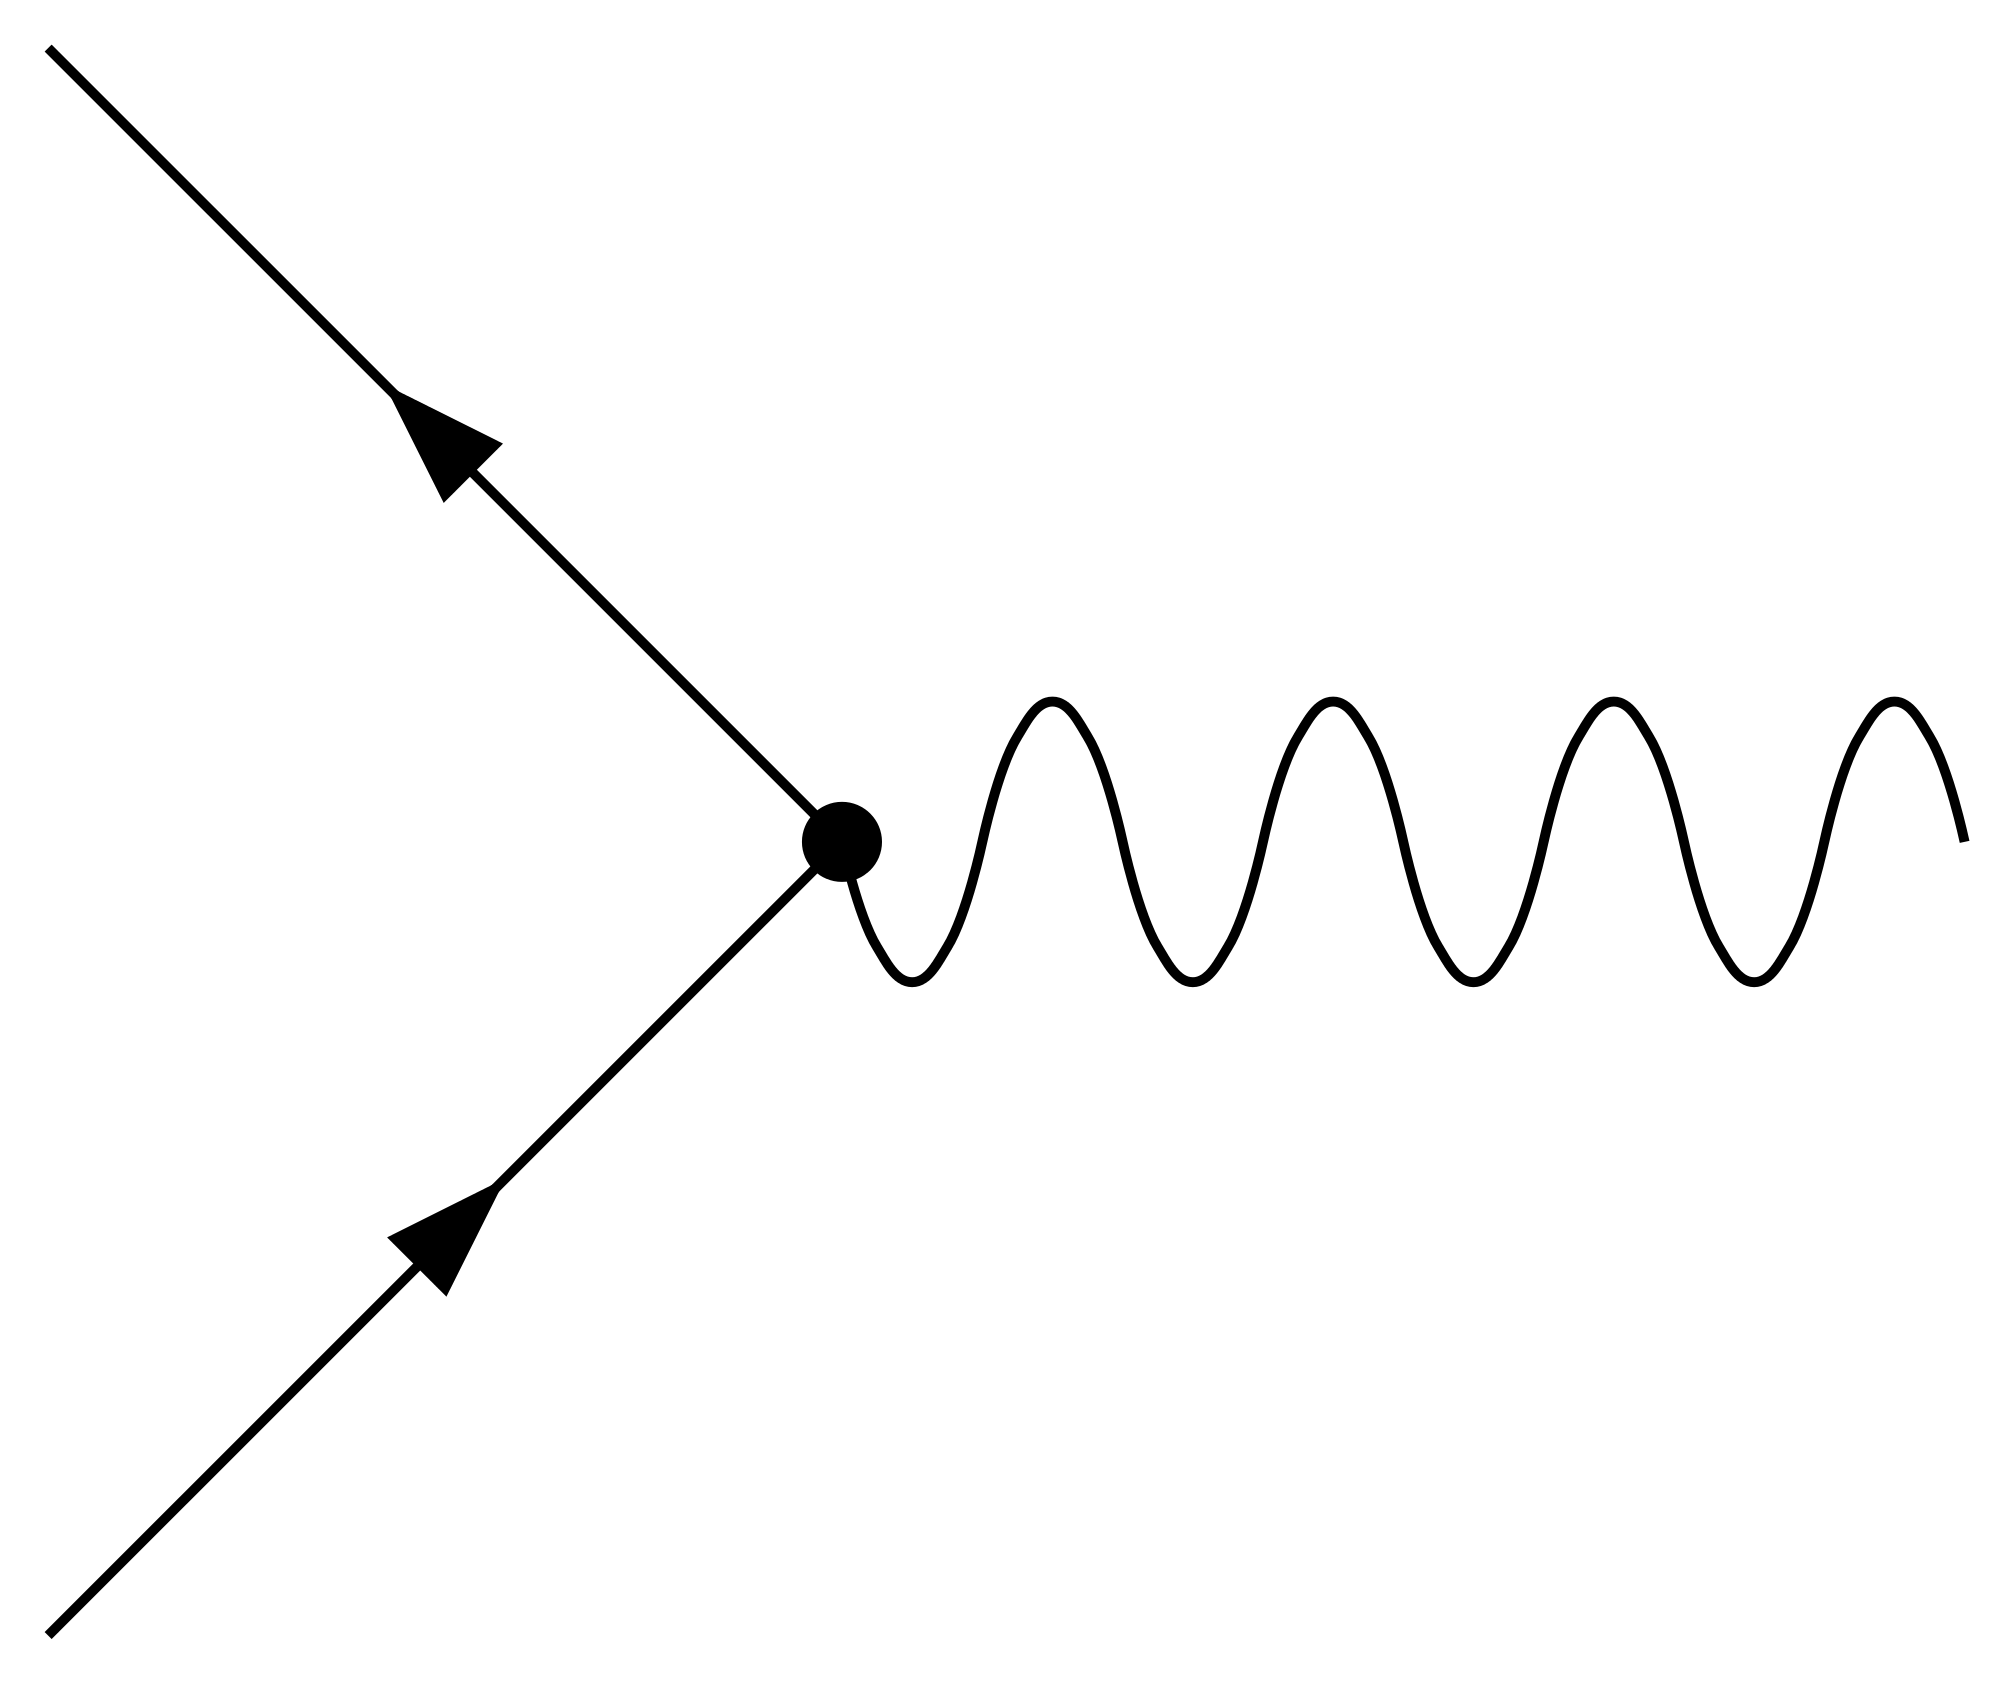
\includegraphics[width=0.35\textwidth]{images/Theory/QEDvertex.png}
    \caption{Elementary QED vertex}
    \label{fig:QEDvertex}
\end{center}
\end{figure}

% This diagram alone cannot occur as it violates conservation of energy but it can be used to build a full Feynman diagram for a particle physics process.
The QED Lagrangian can be found in Eq.~\ref{eqn:QEDL} with $D_{\mu}$ representing the covariant derivative which is defined as $D_{\mu} = \partial_{\mu} + iqA_{\mu}$ and $\psi$ representing a relativistic spin-1/2 field. 
\begin{equation}
\mathcal{L} = \overline{\psi}\left(i\gamma^{\mu}D_{\mu}-m\right)\psi - \frac{1}{4}F_{\mu\nu}F^{\mu\nu}
\label{eqn:QEDL}
\end{equation}
Here $q$ represents the charge of the particle and $A^{\mu}$ is the massless field of the electromagnetic four-potential. The Dirac Lagrangian is manifestly invariant to global phase transformations $\psi \rightarrow e^{i\theta} \psi$. The supplementation by $iqA_{\mu}$ is required to make the Lagrangian invariant to local phase transformations $\psi \rightarrow e^{i\theta(x)} \psi$ where $A_{\mu}$ transforms as $A_{\mu} \rightarrow A_{\mu} + \partial_{\mu}\theta(x)$. Hence, the QED Lagrangian is gauge invariant under U(1) phase transformations, where U(1) is the unitary group of complex numbers. 

The mass of the particle is represented by $m$ and $F_{\mu\nu} = \partial_{\mu}A_{\nu} - \partial_{\nu}A_{\mu}$ is the electromagnetic field (or Faraday) tensor.

Application of the Euler-Lagrange equations to Eq.~\ref{eqn:QEDL} leads to the derivation of the Dirac Equation shown in Eq.~\ref{Eqn:Dirac}.
% , where $J_{\mu} = \overline{\psi}\gamma_{\mu}\psi$.

\begin{equation}
\left( \gamma^{\mu }\partial _{\mu } -m - iq\gamma^{\mu }A_{\mu}\right)\psi = 0
\label{Eqn:Dirac}
\end{equation}

The Dirac equation describes the motion for spin-1/2 particles with mass, ie. quarks and charged leptons. From this equation the Feynman rules for QED can be derived. These rules allow the computation of a number, known as the \emph{amplitude}, for each Feynman diagram. The sum total of the amplitudes for all diagrams which represent a particular process can be summed to produce the probability or \emph{cross section} for that process to occur.

In QED the vacuum acts like a dielectric medium which produces electron-positron pairs where the virtual electron is attracted to positive charges and the virtual positron is repelled (and vice versa for negative charges). This vacuum polarisation partially screens the charged particle and effectively reduces its field. However at short distances, the effective charge increases as the screening reduces.
% \textbf{Effective coupling}

\subsubsection{Weak interactions}

The charged weak interaction is the only interaction where a flavour changing process can occur. The diagram of weak nuclear decay in Fig.~\ref{fig:QEDvertex} illustrates the W boson's interaction with different flavour quarks and leptons. The are two W bosons, one of positive charge and one of negative charge, W$^{\pm}$.


\begin{figure}[ht!]
\begin{center}
    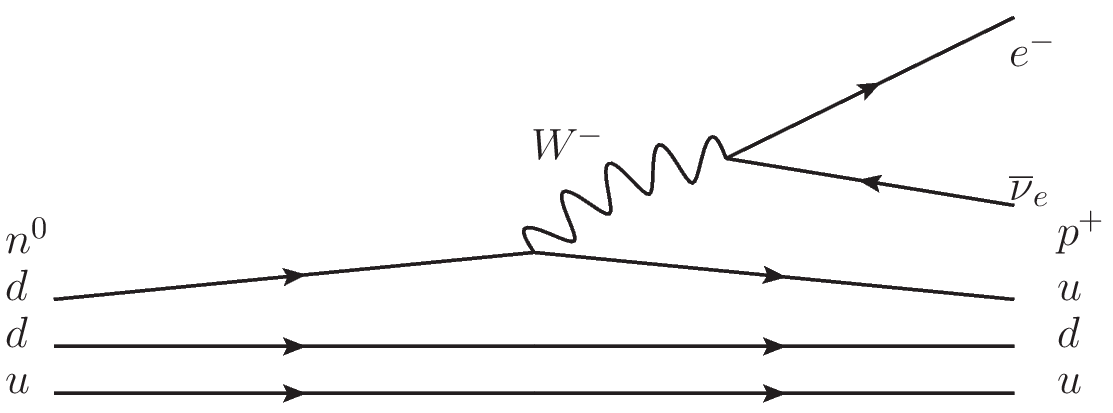
\includegraphics[width=0.65\textwidth]{images/Theory/weakDecay.png}
    \caption{Weak nuclear decay of neutron to proton}
    \label{fig:QEDvertex}
\end{center}
\end{figure}

The neutral weak interaction is mediated by Z bosons which can interact with any quark or lepton as long as the flavour is conserved at the vertex.

% As the weak force bosons are massive, this means that weak decays are much slower than decays via electromagnetism for instance. This means that particles that can only decay via the weak force have longer lifetimes. 
The weak force only interacts with chirality left-handed (right-handed) particles (anti-particles).
% , ie. particles where the spin is (anti-)aligned with the momentum direction. 
The charge for weak interaction is \emph{weak isospin} ($I_{3}$) which is $\pm1/2$ for left-handed fermion, $\pm1$ for W$^{\pm}$ and zero otherwise.

Weak interactions are the only interactions known to violate parity conservation, which was hypothesised by Yang and Lee~\cite{PhysRev.104.254} and experimental validated by Wu in 1957~\cite{PhysRev.105.1413}. It was later discovered that weak interactions also violate the combined charge-parity (CP) symmetry~\cite{Cronin2012,PhysRevLett.13.138}.

\subsubsection{Electroweak Unification}

Glashow~\cite{Glashow:1961tr}, Weinberg~\cite{PhysRevLett.19.1264} and Salam~\cite{Salam:1968rm} formulated the unification of the weak and electromagnetic forces combined in the SU(2)~x~U(1) gauge group. They are hypothesised to merge into one electroweak force above the unification energy of $\approx 100$~GeV. The theory contains four gauge bosons: three W bosons W$_{a}~(a=1,~2,~3)$ and one B boson. Weak hypercharge is defined as $Y_{W} = 2(Q-I_{3})$ and it is $Y_W$ which is the generator of the U(1) component of the electroweak gauge group, which is mediated by the B boson. Equation~\ref{eq:EWK_L} shows the Lagrangian for electroweak interactions where it can be seen that the left-handed fermion fields, represented in the doublet $\psi_{L}$, couple to the W and B bosons and the right-handed fermion fields, $\psi_{R}$, couple to the B boson only. The generators of the SU(2) component are ${\bf T} = \boldsymbol{\sigma}/2$ where $\boldsymbol{\sigma}$ are the Pauli matrices.

\begin{equation}
\label{eq:EWK_L}
\begin{split}
\calL_\textrm{EWK} & = \bar{\psi}_L \gamma^\mu ( i\partial_\mu  - g \mathbf{T} \cdot \mathbf{W}_\mu - \frac{g'}{2} Y_{W}
B_\mu) \psi_L + \\ & + \bar{\psi}_R \gamma^\mu (i \partial_\mu - \frac{g'}{2} Y_{W} B_\mu) \psi_R -
\frac{1}{4}\mathbf{W}_{\mu\nu} \mathbf{W}^{\mu\nu} -\frac{1}{4}B_{\mu\nu} B^{\mu\nu},
\end{split}
\end{equation}

The left-handed doublet, $\psi_L$, can consist of either a left-handed up-type and a left-handed down-type quark or a left-handed neutrino and left-handed charged lepton. The right-handed field, $\psi_R$, can be either a right-handed up-type quark, a right-handed down-type quark, or a right-handed charged lepton. Right-handed neutrinos have not been observed.

\begin{equation*}
\psi_L = \twovector{u_L}{d_L}, \twovector{\nu_L}{\ell_L}~~~~\psi_R=~u_R,~d_R,~\ell_R
\end{equation*}

The spontaneous symmetry breaking mechanism proposed by Brout, Englert~\cite{PhysRevLett.13.321} and Higgs~\cite{PhysRevLett.13.508} results in the linear combination of these 4 bosons into the four more familiar gauge bosons from Table~\ref{table:SMbosons}, W$^{\pm}$, Z and the photon ($\gamma$) as shown in Eqs.~\ref{eqn:Zgamma} \&~\ref{eqn:Wpm}, where $\theta_{W}$ is the weak mixing angle. It is through this mechanism that the W$^{\pm}$, Z bosons gain mass.
\begin{equation}
\label{eqn:Zgamma}
{\begin{pmatrix}
\gamma \\
\textrm{Z} 
\end{pmatrix}}
=
{\begin{pmatrix}
\cos\theta_{W} & \sin\theta_{W} \\
-\sin\theta_{W} & \cos\theta_{W} 
\end{pmatrix}}
{\begin{pmatrix}
\textrm {B} \\
\textrm{W}_{3}
\end{pmatrix}}
\end{equation}

\begin{equation}
\label{eqn:Wpm}
\textrm{W}^{\pm}=\frac{1}{\sqrt{2}}\left(\textrm{W}_{1}\mp i\textrm{W}_{2}\right)
\end{equation}

% Equation~\ref{eqn:EWL} shows the electroweak Lagrangian where $\mathcal{L}_{K}$ gives the kinetic term, $\mathcal{L}_{N}$ gives the neutral interactions and $\mathcal{L}_{C}$ the charged interactions. $\mathcal{L}_{H}$ gives the Higgs three and four point self-interactions and  $\mathcal{L}_{HV}$ gives the Higgs interactions for vector bosons.  $\mathcal{L}_{WWV}$ ($\mathcal{L}_{WWVV}$) gives the three (four) point interactions of the vector bosons and $\mathcal{L}_{Y}$ gives the Yukawa couplings between the Higgs field and the fermions.

% \begin{equation}
% \label{eqn:EWL}
% \mathcal{L}_{EW} = \mathcal{L}_{K} + \mathcal{L}_{N} + \mathcal{L}_{C} + \mathcal{L}_{H} + \mathcal{L}_{HV} + \mathcal{L}_{WWV} + \mathcal{L}_{WWVV} + \mathcal{L}_{Y}
% \end{equation}

% and $\psi_L$ and $\psi_R$ are summed over all possibilities shown in Equations~\ref{eq:lepton_EWK_fields} and
% \ref{eq:quark_EWK_fields}.

% The Yukawa couplings, which describe the couplings between dirac fields and a scalar field, 

After electroweak symmetry breaking, where the Higgs boson gets a vacuum expectation value, the electroweak Lagrangian changes form as described in Ref~\cite{Pich:2005mk}. It now has a kinetic term, a term for the neutral interactions and one for the charged interactions. One term for the Higgs three and four point self-interactions and another term for the Higgs interactions with vector bosons. There is a term for both the three and four point interactions of the vector bosons and another term for the Yukawa couplings between the Higgs field and the fermions. It is through the spontaneous symmetry breaking mechanism that the Yukawa term gains mass terms for fermions as shown in Eq.~\ref{eqn:yukawaMass}, where $M_f$ is the mass of the fermion, $Y_f$ is the Yukawa coupling and $v$ is the vacuum expectation value.

\begin{equation}
M_f = Y_f \frac{v}{\sqrt{2}}
\label{eqn:yukawaMass}
\end{equation}
% \begin{equation}
% \label{eqn:EWL2}
% \mathcal{L}_{EW} = \mathcal{L}_{K} + \mathcal{L}_{N} + \mathcal{L}_{C} + \mathcal{L}_{H} + \mathcal{L}_{HV} + \mathcal{L}_{WWV} + \mathcal{L}_{WWVV} + \mathcal{L}_{Y}
% \end{equation}

The charged current interaction is particularly interesting for the W decays from top quarks. It is described by the term in Eq.~\ref{eqn:CCint}, where $\psi_L$ is now rotated from flavour eigenstate to the weak eigenstate,.

\begin{equation}
\label{eqn:CCint}
\mathcal{L}_{C} = \frac{g}{\sqrt{2}} i\bar{\psi_{L}} \gamma^{\mu} \partial_{\mu} \psi_{L}
\end{equation}
\begin{equation*}
\psi_L = \twovector{u_L}{{d'}_L}, \twovector{\nu_L}{l_L}
\end{equation*}

The weak eigenstates are related to the flavour eigenstates through the CKM matrix, $V_{CKM}$, via ${d^{\prime}}_L = V_{CKM}~d_L$, where ${d^{\prime}}_L$ is a superposition of the flavour eigenstates. The CKM matrix, also known as the \emph{quark mixing matrix}, is a unitary matrix which describes the strength of the couplings for weak decays and it is shown in Eq.~\ref{eqn:CKM1}. 
\begin{equation}
\label{eqn:CKM1}
{\begin{pmatrix}
d^{\prime }\\
s^{\prime }\\
b^{\prime }
\end{pmatrix}}
=
{\begin{pmatrix}
V_{ud}&V_{us}&V_{ub}\\
V_{cd}&V_{cs}&V_{cb}\\
V_{td}&V_{ts}&V_{tb}
\end{pmatrix}}
{\begin{pmatrix}d\\s\\b
\end{pmatrix}}
\end{equation}
The probabilities for the up-type quarks to transition to down-type quarks are given in Eq.~\ref{eqn:CKM2}.
\begin{equation}
\label{eqn:CKM2}
{\begin{pmatrix}
|V_{ud}|&|V_{us}|&|V_{ub}|\\|V_{cd}|&|V_{cs}|&|V_{cb}|\\|V_{td}|&|V_{ts}|&|V_{tb}|
\end{pmatrix}}
=
{\begin{pmatrix}0.97417\pm 0.00021 & 0.2248\pm 0.0006 & 0.00409\pm{0.00039}\\
0.220\pm 0.005 & 0.995\pm 0.016 & 0.0405\pm{0.0015}\\
0.0082\pm{0.0006} & 0.040\pm{0.0027}&1.009\pm0.031
\end{pmatrix}}
\end{equation}



\subsection{Quantum chromodynamics}

Quantum chromodynamics (QCD) is a non-Abelian gauge theory based on the SU(3) symmetry group that describes the strong interactions between quarks and gluons. Quarks and gluons carry colour charge. Each (anti-)quark will carry one of \\(anti-)~red, (anti-)~green or (anti-)~blue colour charge whilst there are 8 types of gluon which exist in a superposition of colour-anti-colour states. One of the elementary QCD vertices is shown in Fig~\ref{fig:QCDvertex} where two quarks couple to a gluon. There are also three and four-point interactions between gluons.
\label{subsec:QCD}
\begin{figure}[ht!]
\begin{center}
    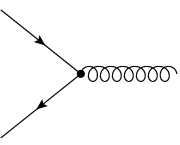
\includegraphics[width=0.35\textwidth]{images/Theory/QCDvertex.png}
    \caption{An elementary QCD vertex}
    \label{fig:QCDvertex}
\end{center}
\end{figure}


Equation~\ref{eqn:QCDL} gives the QCD lagrangian, $\mathcal{L}_{\textrm {QCD}}$ , where $G_{\mu \nu }^{a}=\partial _{\mu }{\mathcal {A}}_{\nu }^{a}-\partial _{\nu }{\mathcal {A}}_{\mu }^{a}+gf^{abc}{\mathcal {A}}_{\mu }^{b}{\mathcal {A}}_{\nu }^{c}$ is the gluon field strength tensor and $f^{abc}$ are the structure constants of SU(3).
\begin{equation}
    \label{eqn:QCDL}
{\mathcal {L}}_{\mathrm {QCD} }={\bar {\psi }}_{i}\left(i(\gamma ^{\mu }D_{\mu })_{ij}-m\,\delta _{ij}\right)\psi _{j}-{\frac {1}{4}}G_{\mu \nu }^{a}G_{a}^{\mu \nu }
\end{equation}

\textbf{Asymptotic freedom and colour confinement}\\
Quark-anti-quark loops lead to screening of the quark colour charge, however gluon loops contribute the opposite by `anti-screening'. It was found that in any theory with $11n>2f$, where $n$ is the number of colours and $f$ is the number of quark flavours, the coupling constant, $\alpha_{S}\left( |q^{2}| \right)$, will decrease with increasing energy, q$^{2}$~\cite{PhysRevLett.30.1343,PhysRevLett.30.1346}. This is known as \emph{asymptotic freedom} as the quarks inside hadrons effectively act like free particles. This is in contrast to QED where there is no `anti-screening' effect.

% \begin{equation}
% \label{eqn:alphaSQCD}
% \alpha_{S}\left( |q^{2}| \right) = \frac{\alpha_{S}\left( \mu^{2} \right)} {1 + \left[ \alpha_{S}\left( \mu^{2} \right)/12\pi \right]\left( 11n -2f \right) \ln \left(|q^{2}|/\mu^{2}\right)}
% \end{equation}

At larger distances the strong force increases, hence energy which has gone into separating two quarks reaches a critical point where it is transferred into producing more quarks which accompany the separated quarks to form hadrons. This is the principle of \emph{confinement} and it ensures that colour doublets or octets are never found in nature, only colour singlet states such as mesons and baryons. The showering of separated quarks into hadrons is called \emph{hadronisation}. This is in contrast, again, to QED where particles can carry electric charge.


\section{Proton-proton collisions}
% At a lepton collider, one can assume that the initial particles involved in a collision are fundamental particles which means precise details of the initial state are known. However 
At the Large Hadron Collider (LHC) the particles involved in the collisions are protons, which are complex composite particles consisting of three valence quarks (two up quarks and one down quark) and gluons which exchange the strong force, as well as `sea quarks' which are quark-anti-quark pairs that come into and out existence rapidly and continuously within the proton.

Figure~\ref{fig:protonPDF} shows the parton distribution functions for the proton. These are interpreted as the probability for a quark to be carrying a fraction, $x$, of the proton's momentum in the longitudinal direction.

\begin{figure}[ht!]
\begin{center}
    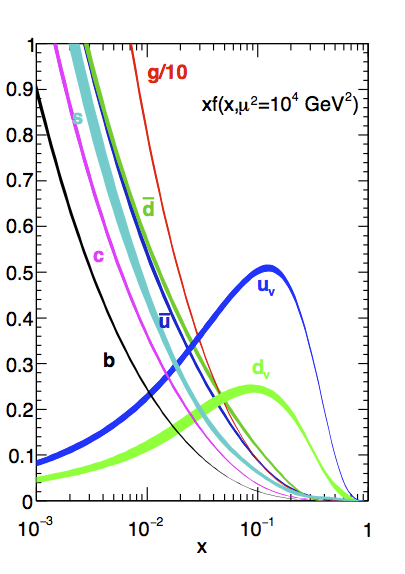
\includegraphics[width=0.65\textwidth]{images/Theory/pdfnob.png}
    \caption{Proton parton distribution functions $xf(x)$ $(f = u_{v},~ d_{v},~ \overline{u},~ \overline{d},~ s\approx\overline{s},~ c\approx\overline{c},~ b\approx\overline{b},~ g$ ) for a given momentum fraction, $x$. Obtained from NNLO NNPDF3.0~\cite{Ball2015}}
    \label{fig:protonPDF}
\end{center}
\end{figure}

Protons in the LHC may a) not interact at all and continue to be accelerated around the ring, b) interact via a soft scatter where the products mostly travel along the direction of the beam, c) participate in a hard interaction where two partons within the protons have a high energy collision in which the products travel transverse to the beam. In the latter case, the remaining partons which have not participated in the hard interaction hadronise and form what is known as the \emph{underlying event} (UE)

\section{Top physics}
The top quark was discovered in 1995 at the Tevatron by the CDF~\cite{PhysRevLett.74.2626} and D0~\cite{Abachi:1995iq} collaborations. It had been hypothesised that there must be a partner to the bottom quark which exists with it in a weak-isospin doublet~\cite{Kobayashi:1973fv}. It is the heaviest quark with a mass of $173.21\pm0.51\pm0.71$~GeV, approximately equivalent to the mass of a rhenium atom\footnote{Atomic number, $Z = 75$}. The top quark is the only quark which predominantly decays before it can form any bound states, due to its short lifetime of $5\times10^{-25}$~seconds~\cite{PDG2016} and hence it is the only quark which can be studied for its spin and polarisation properties. The main decay mode for top quarks is to a bottom quark and a W boson, as shown in Fig.~\ref{fig:tdecay}, which occurs $99.8\pm3.8\textrm{ (exp.)}\pm1.6\textrm {(theo.)} \%$~\cite{2014arXiv1403.7366C} of the time.
 % charged lepton tends to point along the direction of top spin
\begin{figure}[ht!]
\begin{center}
    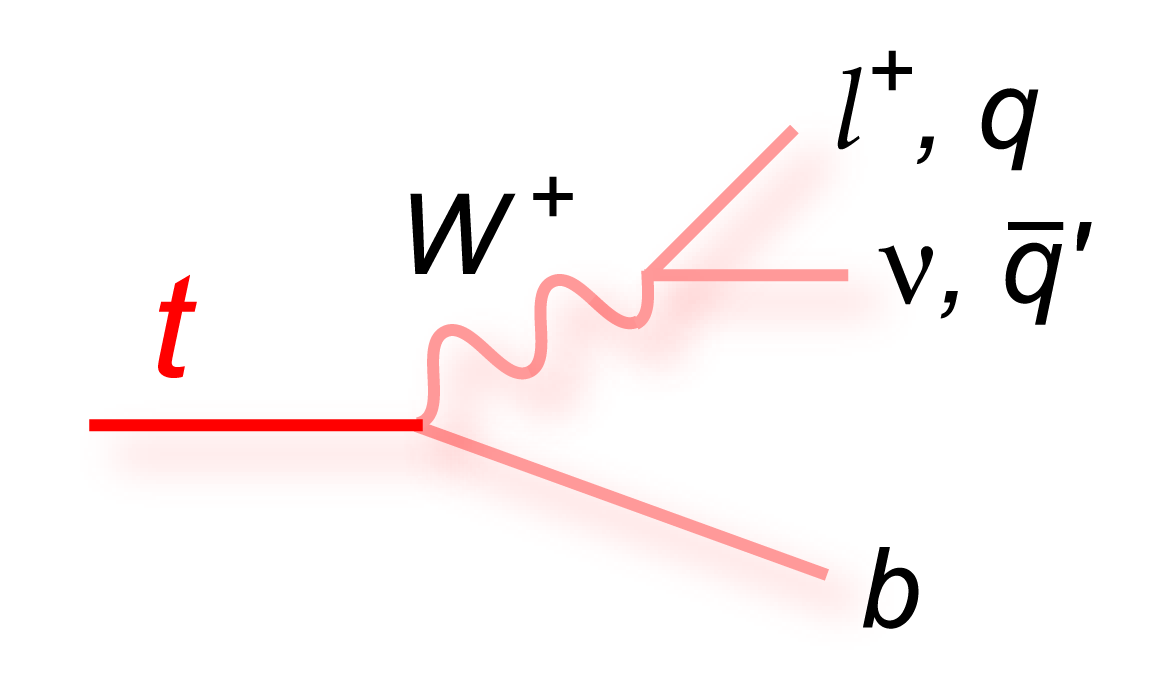
\includegraphics[width=0.49\textwidth]{images/Theory/topdecay.png}
    \caption{Top quark decay to a W boson and b-quark with subsequent decay of the W boson either leptonically or hadronically~\cite{tdecaysource}.}
    \label{fig:tdecay}
\end{center}
\end{figure}

The top quark has the largest Yukawa coupling to the Higgs boson which is of the order of unity. The value of the top quark Yukawa coupling is important in calculations of the stability of the universe and of the energy scales where new physics may arise~\cite{Bezrukov:2014ina}.

\subsection{Top quark pair production}

The first observations of top quarks were made on analyses of top pair production (\ttbar) as this is the dominant mechanism for producing top quarks at hadron colliders. Figure~\ref{fig:ttproduction} shows the leading order tree-level production mechanisms via gluon fusion and quark-anti-quark annihilation. 
%The Feynman rules can be used to calculate the amplitude for each diagram and the summation of the amplitudes gives the theoretical cross section at leading order. 

\begin{figure}[ht!]
\begin{center}
    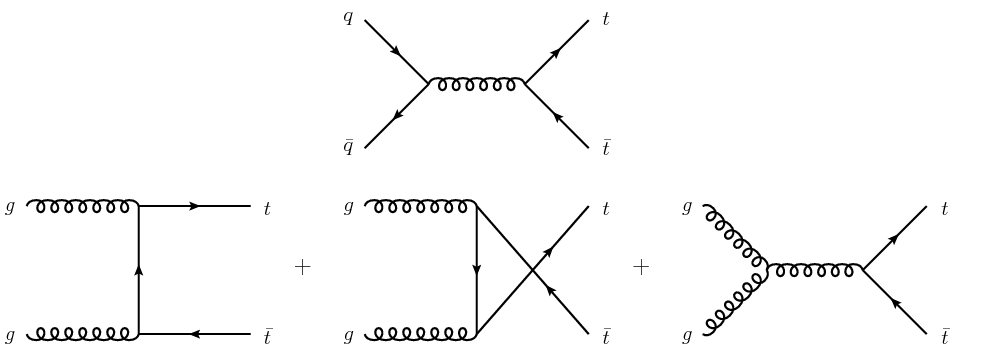
\includegraphics[width=0.95\textwidth]{images/Theory/ttbarfeynman.png}
    \caption{Top quark pair production in the SM by quark-anti-quark annihilation (top) and via gluon fusion (bottom)~\cite{Kohn:2012ksa}}
    \label{fig:ttproduction}
\end{center}
\end{figure}

There are three possible decay modes depending how each top quark decays, as shown in Fig.~\ref{fig:tdecay}: \emph{hadronic} where both W bosons from the top decays decay to a quark and anti-quark, \emph{semi-leptonic} where one W boson decays to \qqbar and one W boson decays to a lepton and a neutrino, and \emph{dileptonic} where both W bosons decay to a lepton and a neutrino each.


\subsection{Single top quark production}

Single top quark production is much rarer than \ttbar production in the SM. It can occur via \qqbar annihilation, g\cPq~fusion or gluon fusion as shown in Fig.~\ref{fig:stFeyn}. In this figure the s-channel (left), t-channel (middle) and associated production with a W boson (tW-channel) are shown.

\begin{figure}[ht!]
\begin{center}
    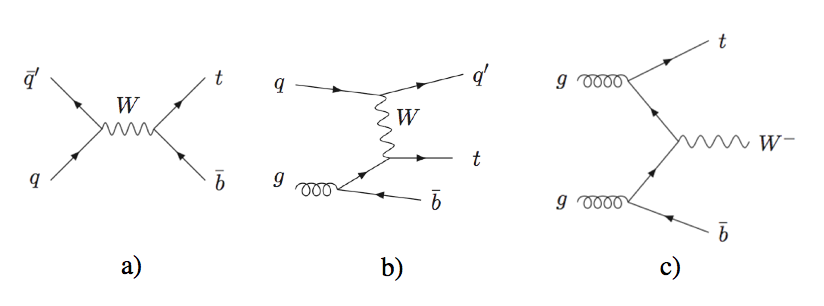
\includegraphics[width=\textwidth]{images/Theory/stFeyn.png}
    \caption{Single top leading order diagrams in the a) s-channel , b) t-channel and c) tW-channel~\cite{Lannon:2012fp}}
    \label{fig:stFeyn}
\end{center}
\end{figure}

The CKM element $|V_{tb}|$ from Eq.~\ref{eqn:CKM2} can be extracted from single top quark decays and the spin of the top quark can be ascertained by studying the leptonic decay of the single top as the charged lepton will point along the direction of the top spin~\cite{Boos:2012hi}.

\subsection{Four top quark production}

The production of four top quarks (\tttt) occurs predominantly via gluon fusion, as seen at leading order in Fig.~\ref{fig:ttttAtLO}, with a $10\%$ contribution from quark-anti-quark annihilation. The production mechanism occurs via QCD whereas the decay of top quarks via W bosons is a weak interaction. 

\begin{figure}[ht!]
\begin{center}
    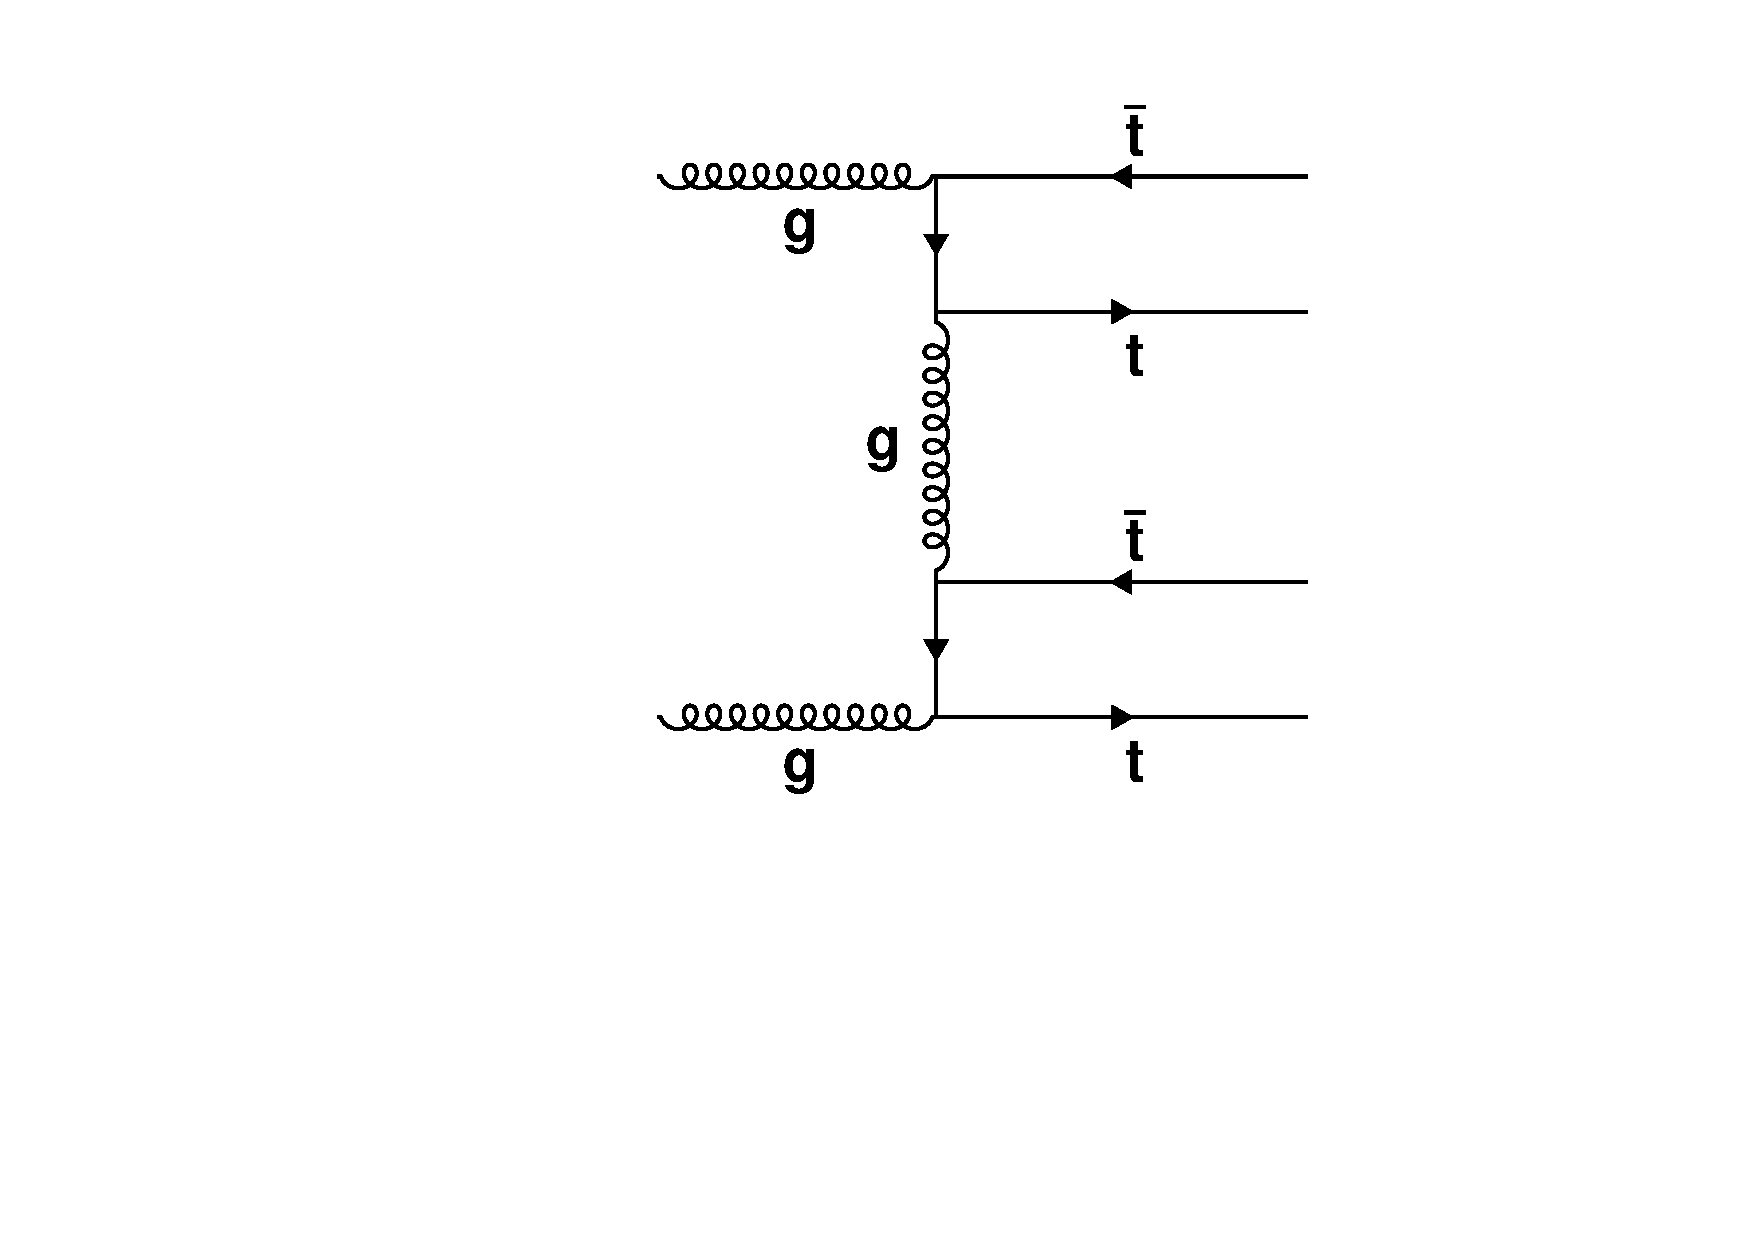
\includegraphics[width=0.49\textwidth]{images/Theory/tttt_t_LO.pdf}
    \caption{Dominant production mechanism of \tttt in the SM.}
    \label{fig:ttttAtLO}
\end{center}
\end{figure}

Final states are determined by the decay of the W bosons which can occur either leptonically or hadronically as seen in Fig.~\ref{fig:tdecay}. 

\section{Shortcomings in the standard model ~\label{sec:SMprobs}}
The SM has been resilient to many tests at the LHC, however there are many questions about the universe which the SM cannot answer. For instance:\\
{\bf Gravity :} How can gravity be integrated into the SM and is there an associated boson for the gravitational force~\cite{PhysRevLett.107.171101,PhysRevD.82.122001}? \\
{\bf Matter-anti-matter asymmetry :} How did the matter-anti-matter asymmetry in the universe arise when it is predicted that the number of particle and anti-particles should be conserved in SM interactions~\cite{RevModPhys.76.1}?\\
{\bf Hierarchy problem :} The SM does not provide a solution as to why the Higgs mass is so much smaller than the Planck mass. It also does not describe why the quarks and lepton masses have values which span many orders of magnitude.\\
{\bf Neutrino mass :}
The Sudbury Neutrino Observatory (SNO) observed that the flux of electron neutrinos from the sun was $\approx 1/3$ what it was expected to be~\cite{PhysRevC.88.025501}. This can be explained by neutrino oscillations. This means that their mass basis is rotated from their weak-flavour basis and hence neutrinos must have mass, which is not part of the SM.\\
{\bf Dark matter :} Observations of the universe show there is non-baryonic, non-luminous matter which is not accounted for within the SM. Studies of galaxy rotation curves show that the angular velocity is relatively constant with radius when it should decrease, meaning that there is additional dark matter providing a contribution to the mass of galaxies~\cite{Volders,
Jog:2002dg,
Persic:1995ru}. The presence of dark matter can also be inferred by gravitational lensing. The light from distant stars in the background is curved around the strong gravitational presence of a dark matter cloud, which itself cannot be seen~\cite{Einstein,Ellis2010}. 
This can cause arcs of light and repeated patterns of the same galaxy as seen in Fig~\ref{fig:ttbarAdd}.
\begin{figure}[ht!]
\centering
    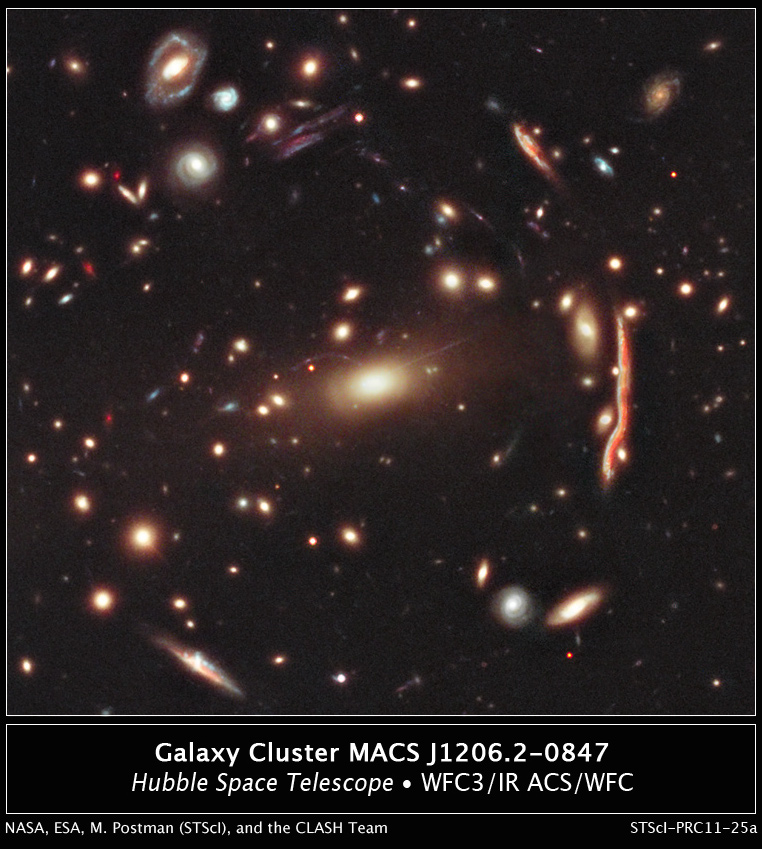
\includegraphics[width=0.65\textwidth]{images/Theory/lensing2.jpg}
    \caption{Gravitational lensing around MACS 1206 as captured by the Hubble Space Telescope~\cite{Glens}}
    \label{fig:Glens}
\end{figure}


\section{BSM models with four top quark signatures ~\label{sec:BSMmodels}}

There are many theories which try to solve some or all of the problems listed in Section~\ref{sec:SMprobs}. Some BSM theories which have final states containing four top quarks are discussed here. 

\textbf{Top quark Compositeness}\\
It has been hypothesised that the top quark could be a composite particle made up of subparticles named preons, which are bound by a new confining force. Phenomenological studies have been performed in which an effective field theory (EFT) is proposed where only the right-handed top quark is considered to be composite. It is argued that if only $t_{R}$ is composite and no other SM component is then the four top operator (shown in Fig~\ref{fig:eft}) will be the most significant component of the EFT lagrangian, which can lead to an enhancement of $\approx 10^3$ to the production of \tttt compared to the SM rate~\cite{Tait2topcomp,Tait1topcomp}.

\begin{figure}[ht!]
\centering
    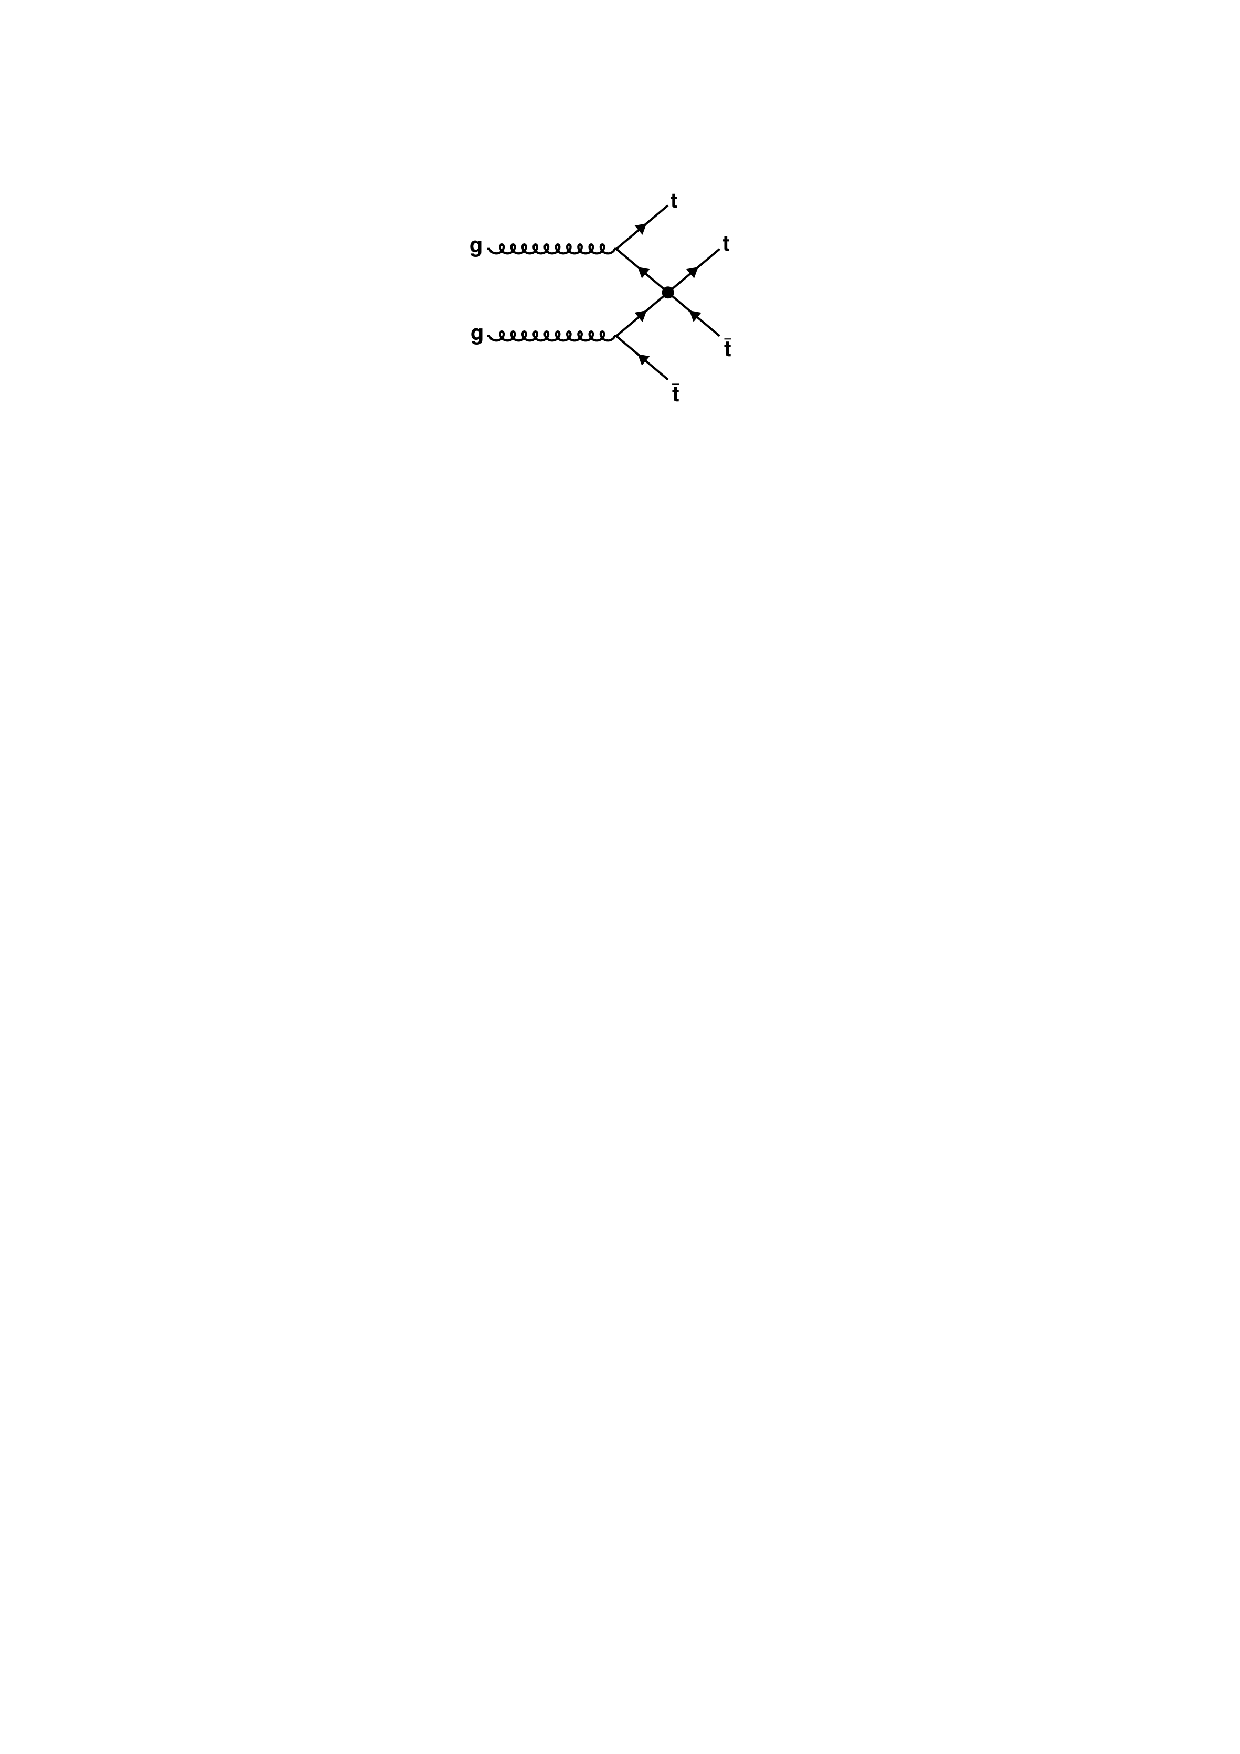
\includegraphics[width=0.45\textwidth]{images/Theory/EFTTopComp.pdf}
    \caption{Four top interaction in an EFT~\cite{Tait2topcomp}}
    \label{fig:eft}
\end{figure}

$\boldsymbol{\ttbar+\textrm{X}, ~\textrm{X}}\rightarrow\boldsymbol{\ttbar}$\\
There are several models which contain \ttbar plus an extra scalar particle which then decays to \ttbar as seen in Fig.~\ref{fig:ttXtt}.
The mediator could be a dark matter mediator~\cite{Arina2016}, a heavy Higgs boson~\cite{Bernreuther:2015fts}, or a member of a scalar colour sextet~\cite{Cacciapaglia2015}, for instance. 

\begin{figure}[ht!]
\centering
    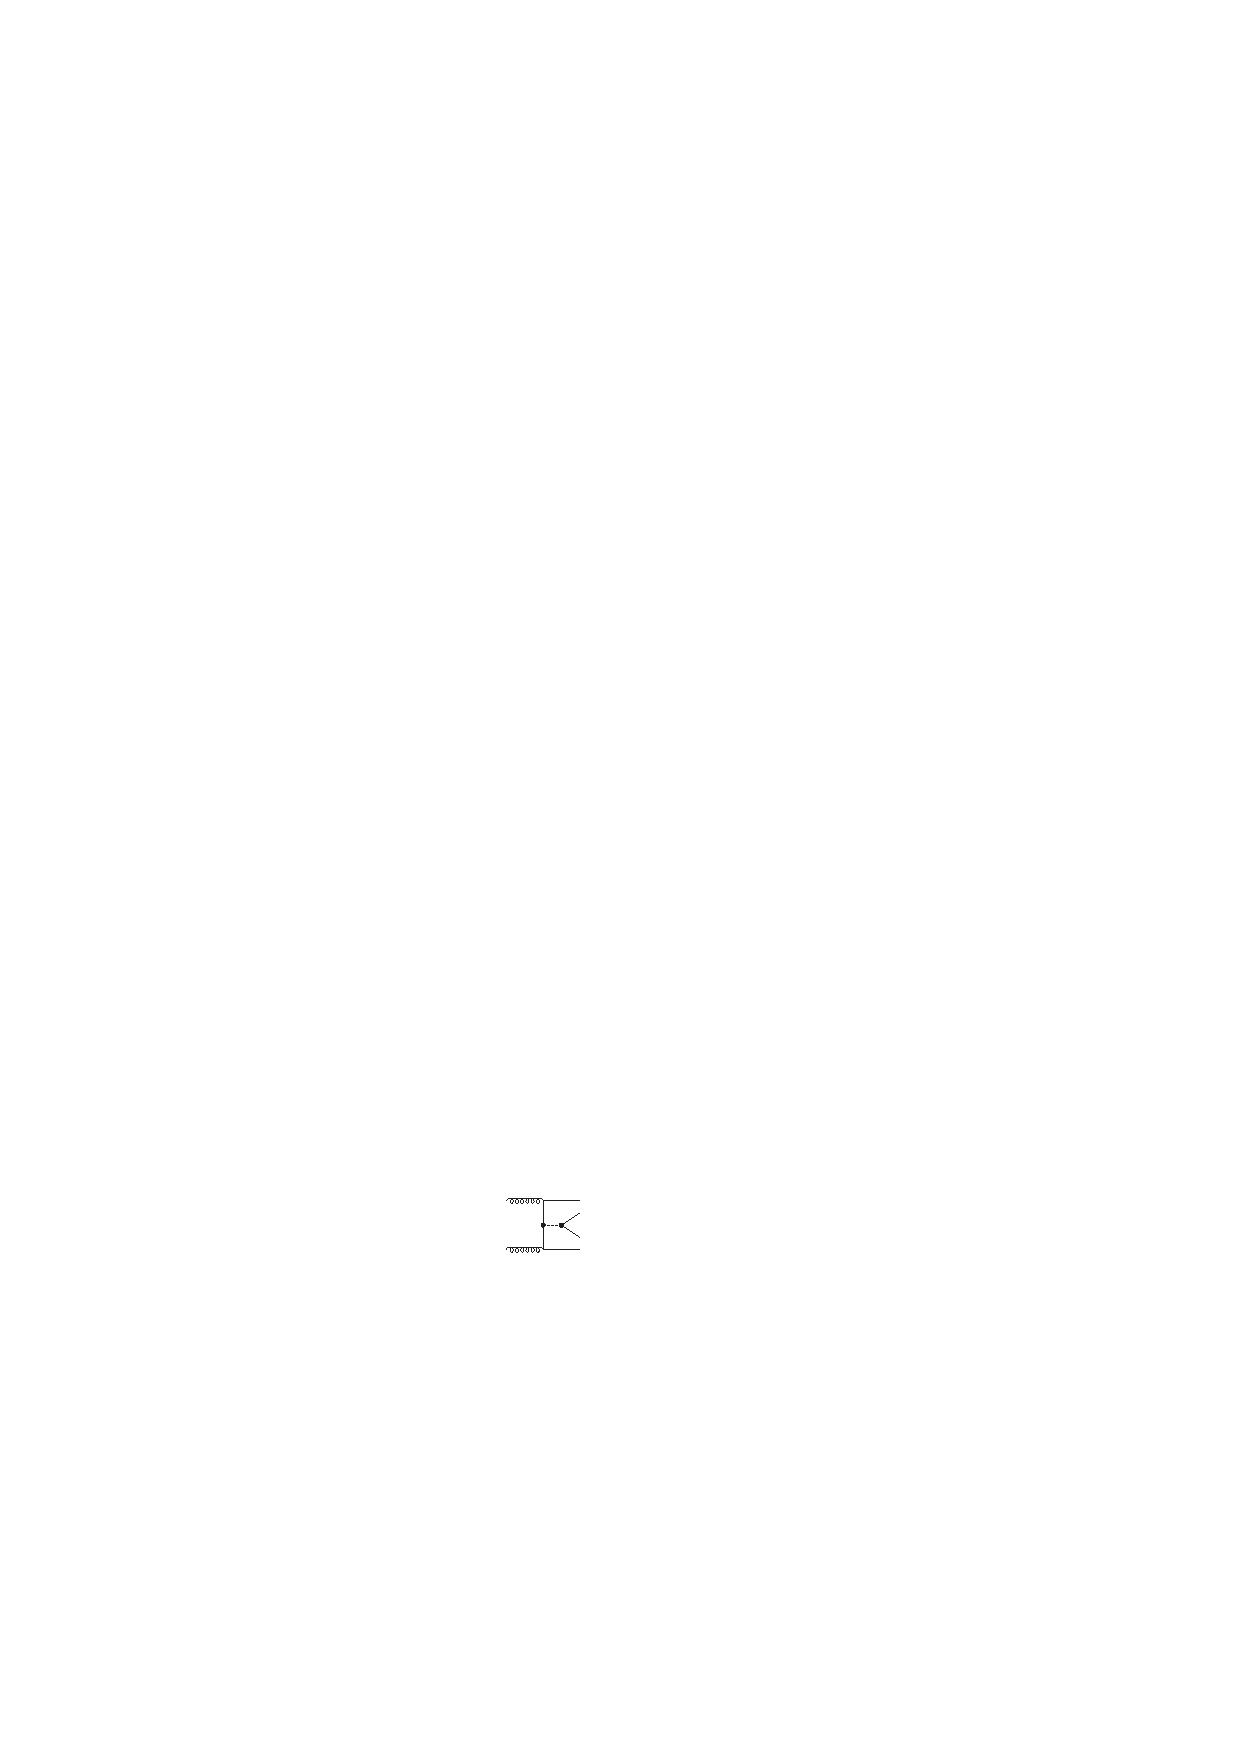
\includegraphics[width=0.45\textwidth]{images/Theory/ttDMtt.pdf}
    \caption{Four top production with an intermediate scalar~\cite{Arina2016}}
    \label{fig:ttXtt}
\end{figure}

% \textbf{Heavy resonances}


\textbf{Scalar pair production to }$\boldsymbol{\tttt}$\\

\begin{figure}[ht!]
\centering
    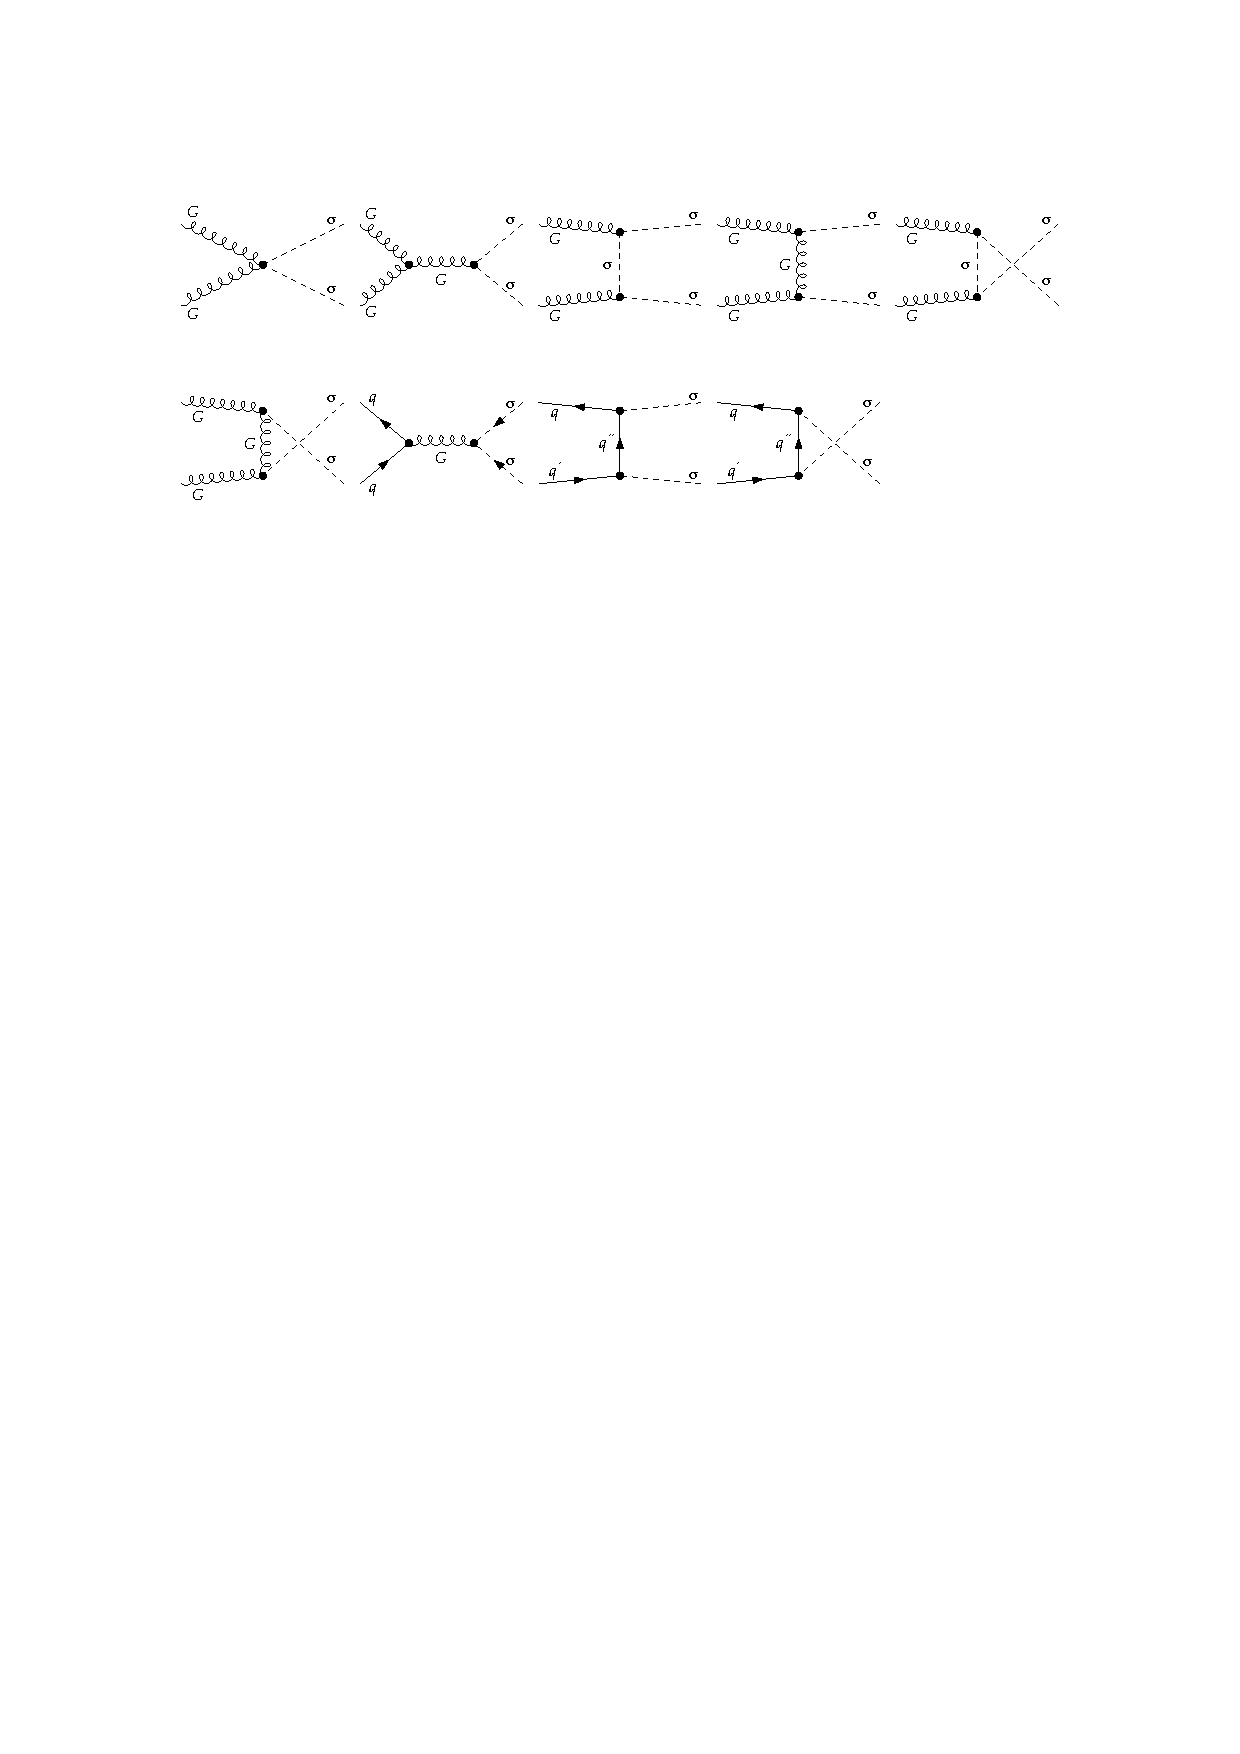
\includegraphics[width=0.99\textwidth]{images/Theory/sgluonFeyn.pdf}
    \caption{Sgluon pair production~\cite{Calvet:2012rk}}
    \label{fig:sgluonpair}
\end{figure}

An additional scalar gluon (\emph{sgluon}) has been theorised in several models of physics beyond the SM. In N=1/N=2 hybrid and R-symmetric versions of non-minimal supersymmetric models (NMSSM), the minimal supersymmetric model (MSSM) is supplemented by an additional chiral multiplet which lies in the adjoint representation of the QCD gauge group. This supermultiplet contains a two-component fermionic part which mixes with the Dirac gluino and a colour-octet complex scalar particle which is the sgluon field. This is particularly interesting because coloured particles will couple directly to gluons and hence should be produced in proton-proton collisions. Figure~\ref{fig:sgluonpair} shows the possible tree level production modes for sgluon pair production.~\cite{Calvet:2012rk}, whilst Fig.~\ref{fig:sgluontttt} shows the each sgluon coupling to a \ttbar resulting in a final state with four top quarks.

\begin{figure}[ht!]
\begin{center}
    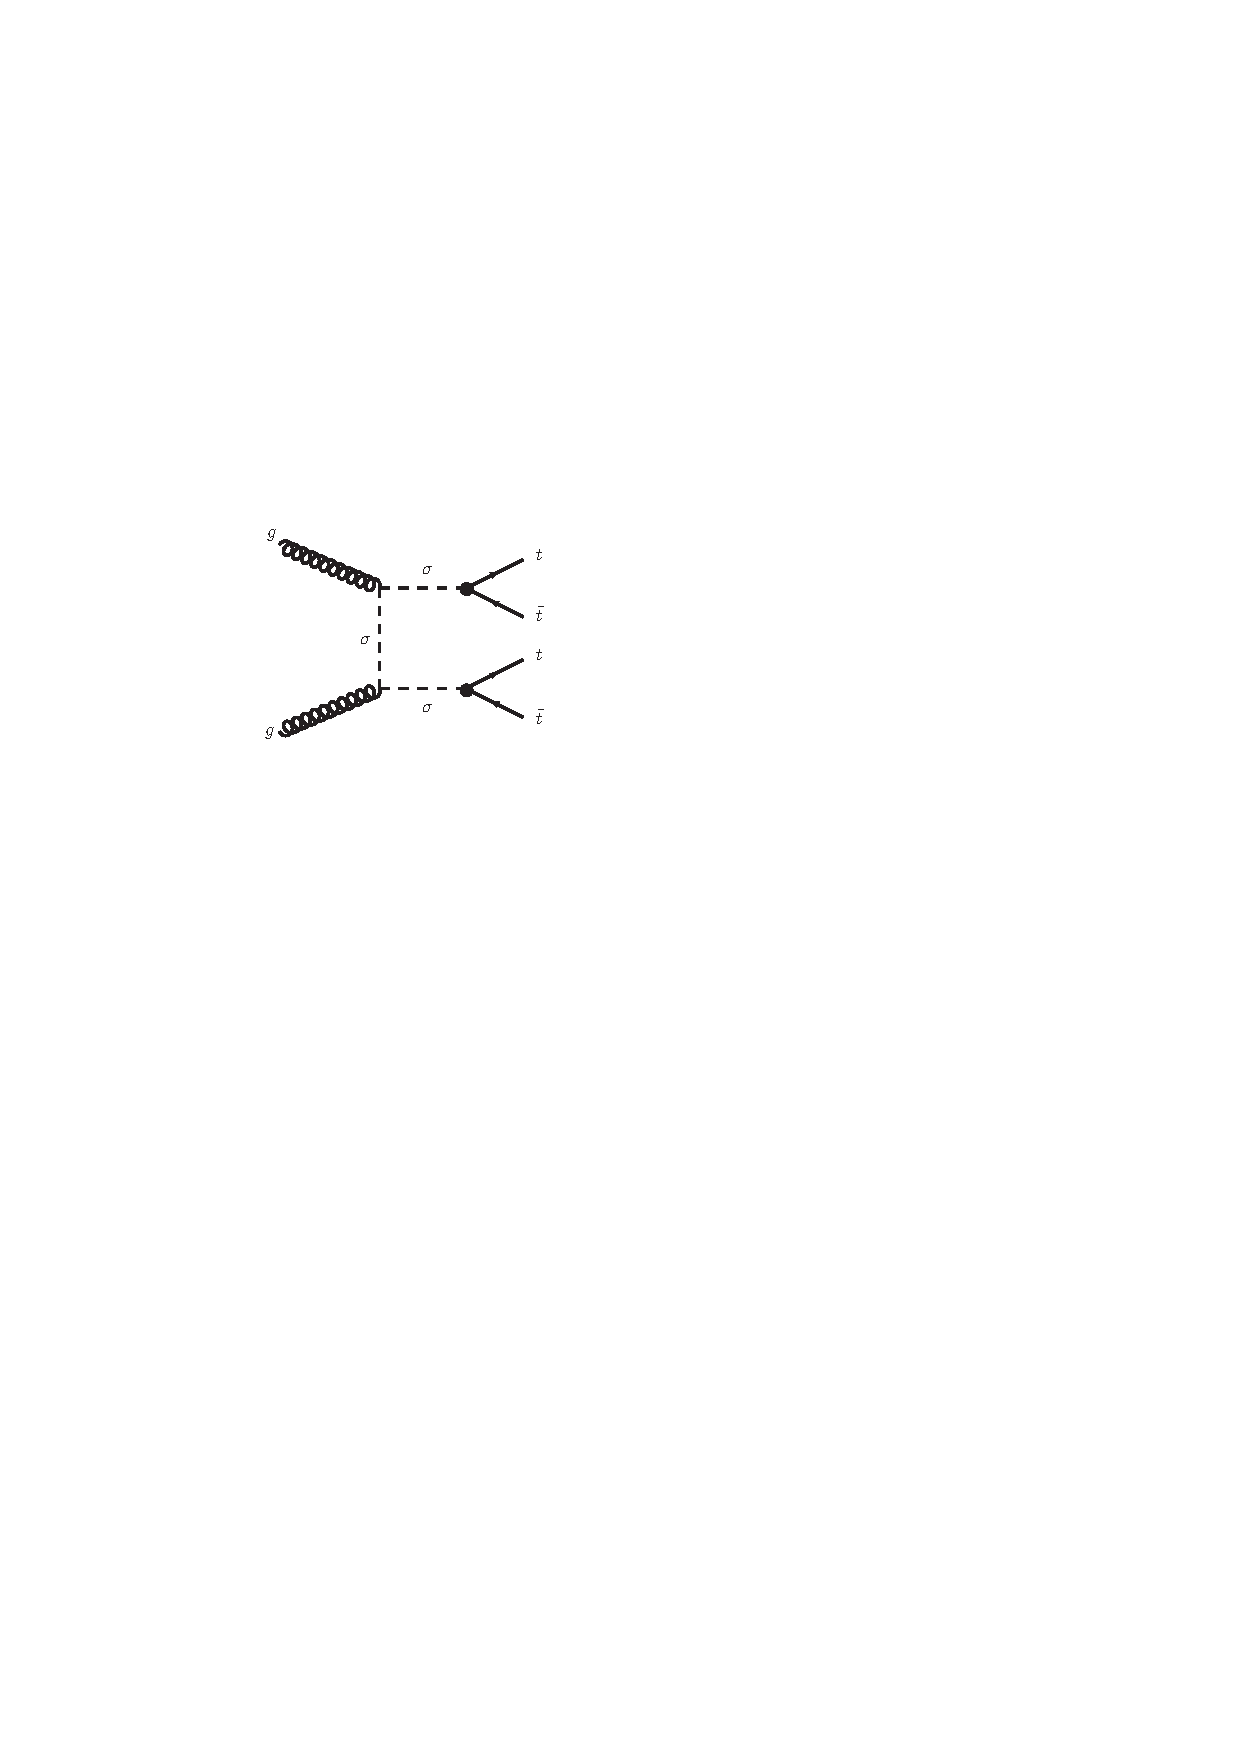
\includegraphics[width=0.49\textwidth]{images/Theory/sgluontotttt.pdf}
    \caption{Sgluon pair production to four-top-quark final state~\cite{Aad:2015kqa}.}
    \label{fig:sgluontttt}
\end{center}
\end{figure}

Sgluons also arise in vector-like confining theories and extra-dimensional models, therefore it is viable to use a simplified model approach (as discussed below) because the final state signatures are reasonably model-independent.

Colour octets and sextets can also be pair produced in theories where the Higgs boson is a composite particle~\cite{Cacciapaglia2015}.



\section{Simplified models}

Simplified models work by building a TeV-scale effective Lagrangian which describes a minimal number of new particles and their interactions. Hence, variables which can be directly observed by the detector can be studied, for example, particle masses, cross sections and branching ratios for different decay modes. Simplified models can sometimes be considered to be a subset of more general physics models where only a few of the particles are considered. Therefore, simplified model cannot be considered to be model independent but they can help to identify the bounds of sensitivity for searches~\cite{0954-3899-39-10-105005}. An example of where a simplified model can be used is in the case of $\ttbar+\textrm{X}$, in Section~\ref{sec:BSMmodels}, where the phenomenology of the resulting particles in the detector can be studied without knowledge of which underlying theory the new scalar particle, X, is coming from.



% \chapter{Top Physics}
\label{c:topPhys}


\section{Top quark physics history}
\fxnote{include ttbar and single}

\section{Four top quark production}

The production of four top quarks occurs predominantly via gluon fusion, as seen at leading order in Fig.~\ref{fig:ttttAtLO}~(left), with a $10\%$ contribution from quark-anti-quark annihilation. The production mechanism occurs via QCD whereas the decay of top quarks via W bosons is a weak interaction. 

\begin{figure}[ht!]
\begin{center}
    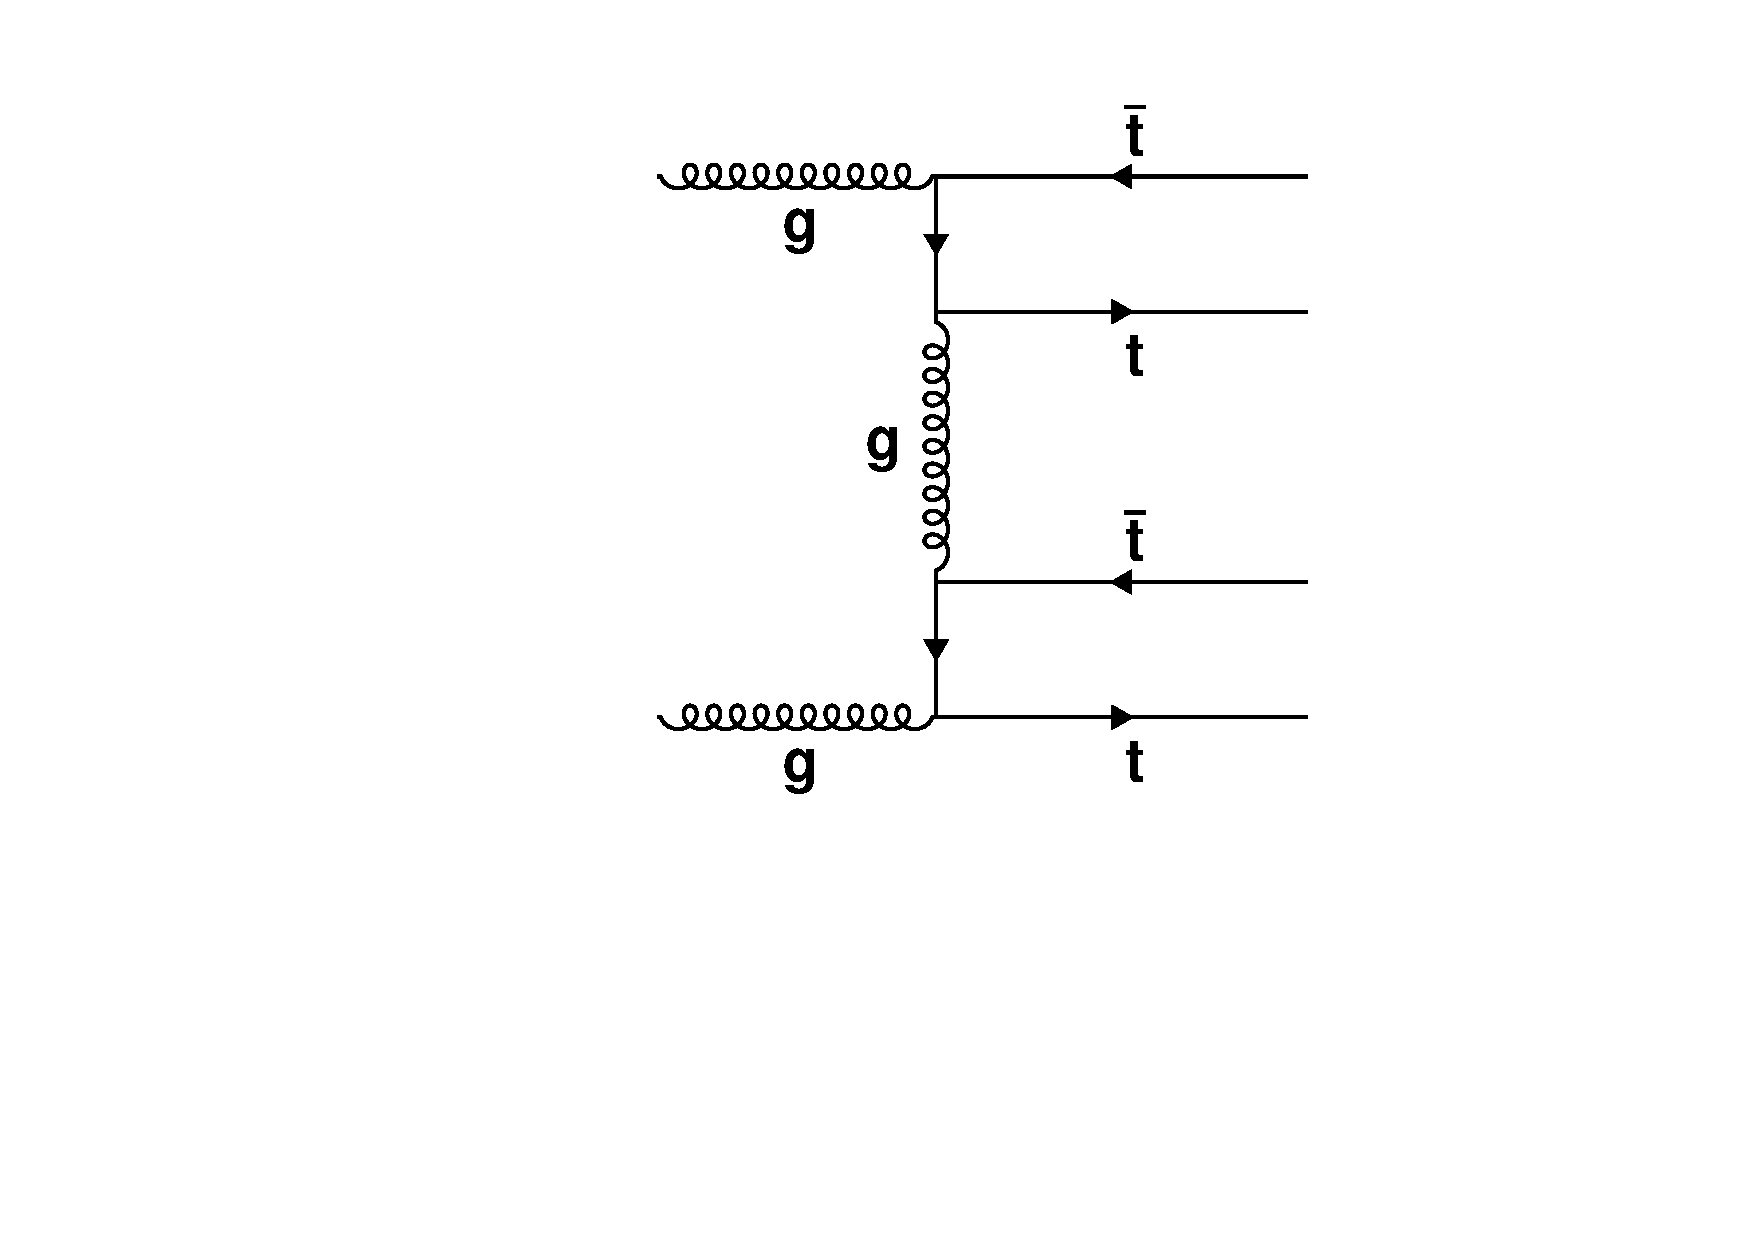
\includegraphics[width=0.49\textwidth]{images/Theory/tttt_t_LO.pdf}
    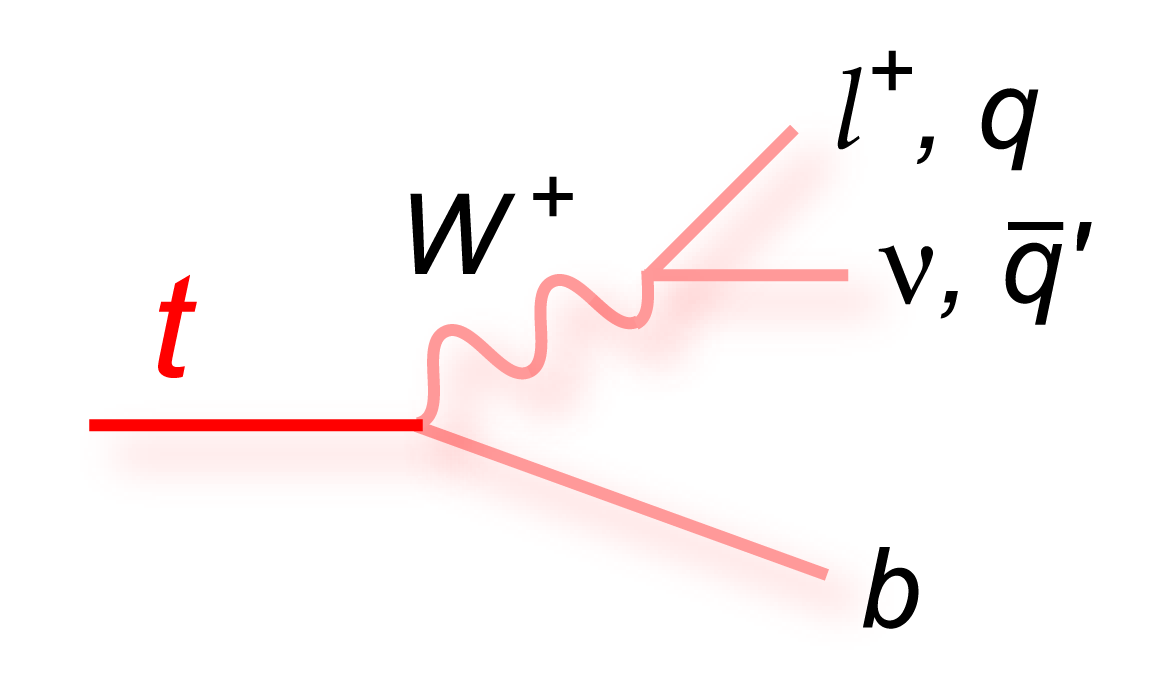
\includegraphics[width=0.49\textwidth]{images/Theory/topdecay.png}
    \caption{Dominant production mechanism for four top quarks in the standard model (left) an top quark decay to a W boson and b-quark with subsequent decay of the W boson either leptonically or hadronically (right).}
    \label{fig:ttttAtLO}
\end{center}
\end{figure}

Final states are determined by the decay of the W boson which can occur either leptonically or hadronically as seen in Fig.~\ref{fig:ttttAtLO}~(right). It can be seen from Fig.~\ref{fig:BRtttt} that the single lepton final state has the largest branching ratio which makes it a favourable place to look to study the largest number of events produced in the CMS detector. This is the final state considered most in this thesis. The dilepton final state also has a large branching ratio and has particularly low backgrounds when same-sign lepton final states are considered. The combination of studies on the dilepton final state will be discussed in Chapter~\ref{c:Run2}.

\begin{figure}[ht!]
\begin{center}
    \includegraphics[width=0.4\textwidth]{images/Theory/FourTopBR.pdf}
    \caption{Branching ratios for final states as defined by leptonic decays.}
    \label{fig:BRtttt}
\end{center}
\end{figure}


%\addcontentsline{toc}{chapter}{Theory}
\chapter{The CMS detector and the Large Hadron Collider}
\label{c:det}
This chapter discusses the Large Hadron Collider (LHC) which is located on the Franco-Swiss border near Geneva approximately 100 m underground at the site of the Conseil Europ\'{e}en pour la Recherche Nucl\'{e}aire (CERN). It is a 26.7 km long synchrotron particle accelerator with four interaction points where four experiments are located.\fixme{TOTEM Moedal CASTOR LHCf}  This thesis focuses on results from the Compact Muon Solenoid detector described in section~\ref{sec:CMSdet}. The other experiments include ATLAS which is a multi-purpose experiment like CMS, the LHCb detector which focusses on the study of the physics of B mesons and the ALICE detector which is used to study the quark-gluon plasma. Details of the function and purpose of each of the CMS sub-detectors are given in this chapter. The algorithms which are used to reconstruct particles from the information given from the sub-detectors is given in chapter~\ref{c:recon}.

\section{LHC}

The LHC accelerates two beams of protons which circulate in opposite directions.
This is achieved using a system of dipole magnets which have an aperture for each beam direction. Quadrapoles are used to squeeze the beam.
The protons are sourced from a bottle of hydrogen where a strong electric field is used to excite the electrons from the hydrogen atom leaving protons behind. The protons are then accelerated through the linear accelerator LINAC2 before being injected into the Proton Synchrotron Booster (PSB), then into the Proton Synchrotron (PS) followed by the Super Proton Synchrotron (SPS) which is the final accelerator before the protons are injected into the LHC ring. Each accelerator stage boosts the protons to a higher energy before they can be injected into the LHC where their final collision energy can be achieved.\fixme{more detail/explain fig3.1}


The protons are accelerated in bunches which are collided at the interaction points of each experiment. This results in many collisions per bunch crossing despite the fact that many protons will miss each other and continue to be accelerated around the LHC. The background of particles coming from the frequent uninteresting collisions is called \emph{Pile up} (PU).

\begin{figure}[ht!]
\centering
    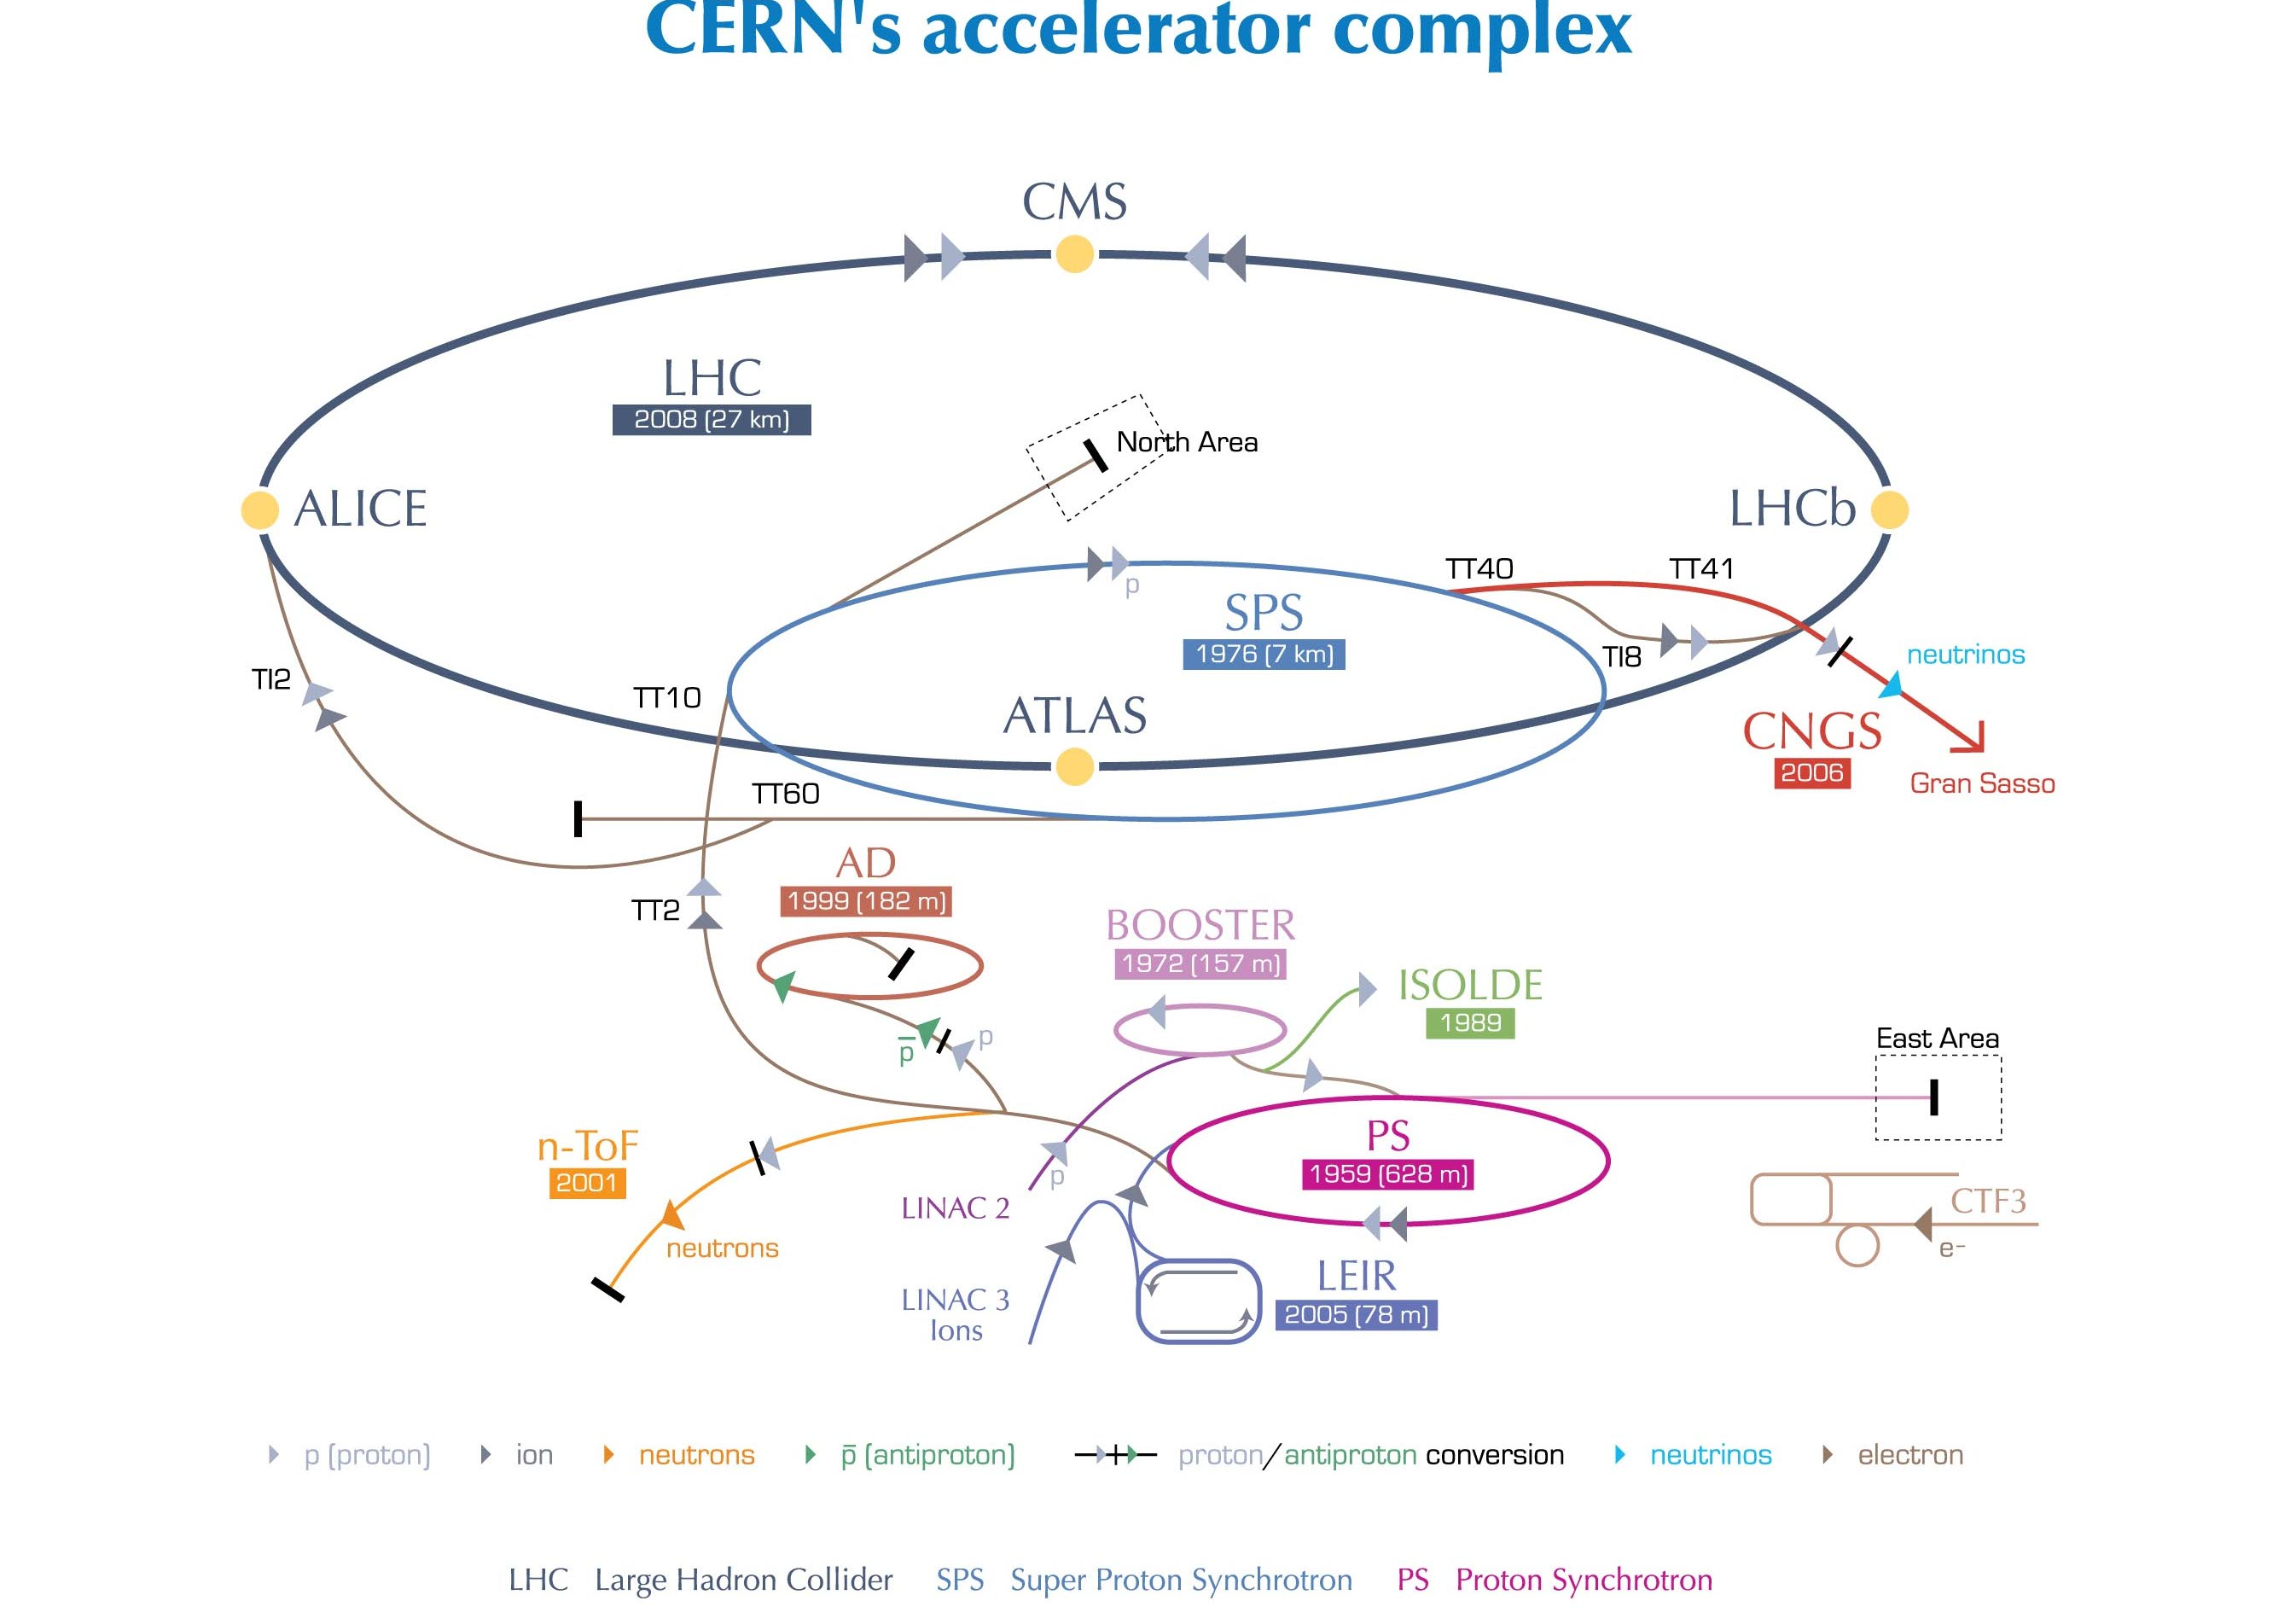
\includegraphics[width=0.95\textwidth]{images/LHCacc.jpg}
    \caption{The LHC accelerator complex at CERN}
    \label{fig:LHC acc}
\end{figure}


The \emph{Luminosity} (\lumi) is a measure of the instantaneous collision rate and can be calculated using equation~\ref{eqn:lumi1}, where f is the bunch frequency, and $N_1$ and $N_2$ are the numbers of particles in each bunch. The effective collision area is $4\pi\sigma_{x}\sigma_{y}$ where $\sigma_{x}$ and $\sigma_{y}$ are the x and y components of the beam, transverse to the beam direction. It is assumed that each beam has the same cross section.

\begin{equation}
\lumi = \frac{f{N}_{1}{N}_{2}}{4\pi\sigma_{x}\sigma_{y}}
\label{eqn:lumi1}
\end{equation}

The \emph{integrated luminosity} (\lumiint) which is shown in Fig~\ref{fig:Lumi} for the CMS experiment from 2010 until 2016 for proton-proton collisions is the delivered luminosity integrated over time. The number of events, $N_{\textrm{events}}$, produced for a particular particle physics process can be calculated from the cross section, $\sigma$, using equation~\ref{eqn:lumi2}.

\begin{equation}
N_{\textrm{events}} = \lumiint \times \sigma
\label{eqn:lumi2}
\end{equation}

\begin{figure}[ht!]
\centering
    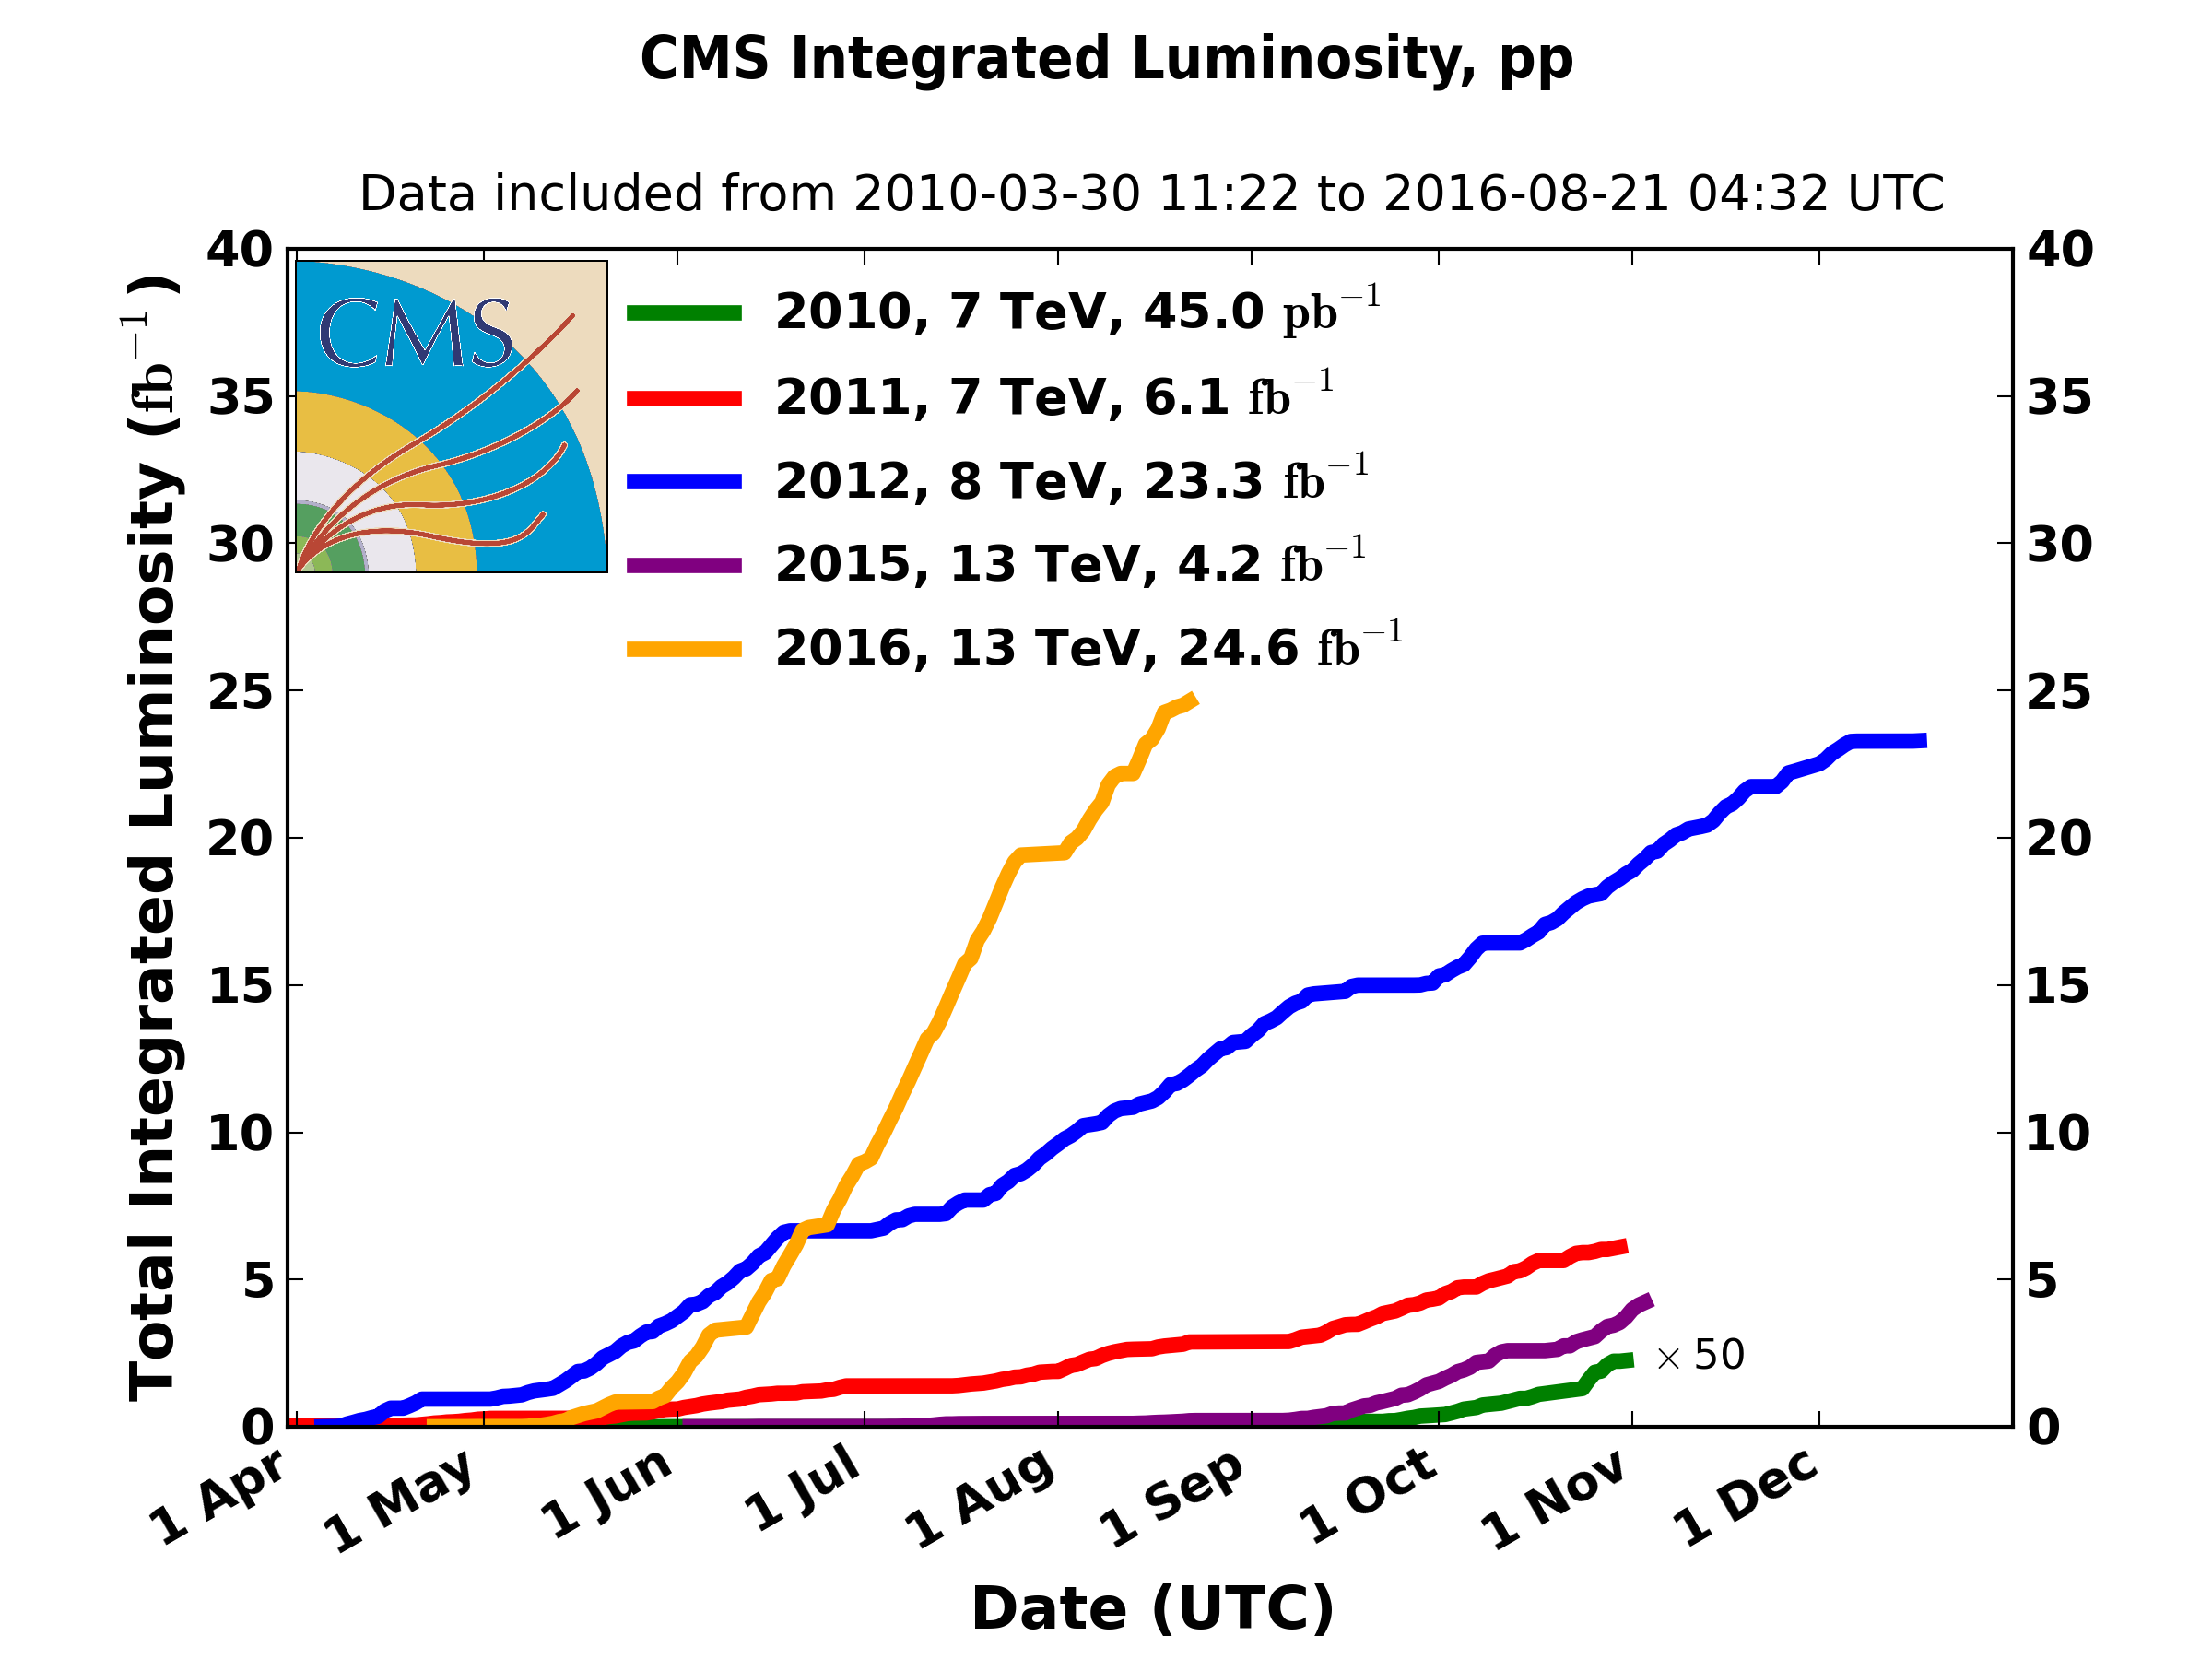
\includegraphics[width=0.95\textwidth]{images/int_lumi_cumulative_pp_2.png}
    \caption{The integrated luminosity in \fbinv for proton-proton collision at the CMS experiment from 2010 to 2016}
    \label{fig:Lumi}
\end{figure}

The LHC was designed to have a centre of mass collision energy of $\sqrt{s} = 14~\TeV$. The intention was to start the machine with a lower energy in September 2008 and to obtain $\sqrt{s} = 10~\TeV$ by the end of 2008. However, an electrical fault 10 days into operation in October 2008 caused damage to over 50 of the superconducting magnets. The LHC was shut down for repairs until November 2009 when LHC achieved the record breaking 1.18 TeV per beam. The centre of mass energy was then ramped up to $\sqrt{s} = 7~\TeV$ in 2011. In 2012 this was increased to $\sqrt{s} = 8~\TeV$ and a dataset with an integrated luminosity of $\approx 20~\fbinv$ was recorded. This dataset from the run phase known as \emph{\runone} was used for the analysis in chapter~\ref{c:Run1}. Further details on the run conditions can be found \fixme*{table of lumi, bunches etc.}{in }. In 2013 after \runone, Long Shutdown 1 (LS1) commenced to make upgrades to the LHC and the detectors to allow the machine to run at $\sqrt{s} = 13~\TeV$ for \emph{\runtwo}. \runtwo began in March 2015 and results from \runtwo are the focus of the analysis in chapter~\ref{c:Run2}.

\runone saw the great success of the discovery of the Higgs boson, one of the main objectives of the LHC~\cite{Aad20121}~\cite{Chatrchyan201230}. In \runtwo, the search for new physics continues where precision measurements, such as the search for the production of four top quarks, will test the predictions of the Standard Model. CMS and ATLAS are considered to be general-purpose detectors which can be used to test many areas of physics within and beyond the standard model. This includes searches for dark matter, \fixme*{more detail run2}{supersymmetric particles...}

\section{CMS detector \label{sec:CMSdet}}

The CMS detector is hermetic detector with a large magnetic solenoid which can deviate particles into curved tracks as they traverse the detector. Closest to the beam line is the silicon tracker which makes the most accurate position measurements. Next are the calorimetry systems for electromagnetic and separately for hadronic particles. All of these detectors are contained within the magnetic solenoid whereas the muon chambers are found finally outside the solenoid where they can measure the muons which are much more pentrating than other particles. The cyclindrical coordinate system of the detector is defined as follows: the x-axis points towards the centre of the LHC ring, the y-axis points upwards and the z-axis points along the beamline in the anti-clockwise direction. The azimuthal angle $\phi$ is measured in the x,y plane clockwise from the x axis. The polar angle $\theta$ is measured clockwise from the z-axis. More commonly the pseudorapidity, defined in equation~\ref{eqn:eta}, is used instead of $\theta$.

\begin{equation}
    \eta = - \ln \left[ \tan \left(\frac{\theta}{2} \right) \right]
    \label{eqn:eta}
\end{equation}

\begin{figure}[ht!]
\centering
    \includegraphics[width=0.95\textwidth]{images/cmsdetector3.pdf}
    \caption{The CMS detector~\cite{1742-6596-513-2-022032}}
    \label{fig:CMSdetector}
\end{figure}


\subsection{Magnetic Solenoid}

The superconducting magnetic solenoid at the core of CMS was designed to have a magnetic field of 4 T. The free bore magnet has a diameter of 6.3 m and length of 12.5 m. It uses 4-layer winding of NbTi superconductor which is required to generate this high magnetic field. The magnet is cooled within a cryostat using liquid helium to a temperature of 4.5K. The magnetic field is returned via an iron yoke consisting of five barrel wheels and two endcaps which are made of three discs each. The outer dimension of the iron flats is 14 m. The tracker, electromagnetic calorimeter and hadronic calorimeter are constrained to be with in the inner dimensions of the solenoid as can be seen in Fig.~\ref{fig:TrackerWhole}. The solenoid provides a homogeneous magnetic field over the tracking region which bends particle trajectories transverse to the beam direction.
% described in section~\ref{sec:tracker}

\subsection{Tracker \label{sec:tracker}}

The tracking system of CMS lies inside the superconducting solenoid and surrounds the interaction point. It is 5.8 m long with a diameter of 2.5 m.
Silicon detectors were used as they can provide the high granulity and fast response required to reliably reconstruct the trajectories of particles coming from the collision vertex before the next collision occurs.
% and from the secondary vertices which originate from decaying particles. 
Reconstructing secondary vertices is also particularly important for identifying jets originating from heavy flavour quarks such as bottom quarks. This is integral for distinguishing final states involving top quarks. The silicon detectors in CMS have been designed to have the radiation hardness to last for the design time of ten years. The minimum material possible was used in order to reduce the amount of multiple scattering, photon conversion and bremsstrahlung. However the high density of electronics means that the tracker requires cooling to zero degrees celcius in \runone and -20 degrees celcius in \runtwo. %Cooling also helps prevent `thermal runaway' from leakage current. 
\fixme{1000 particles 20 PU - overlapping p-p collisions}
%good to limit interaction with material in tracker

The tracking system consists of two main sections; the pixel tracker makes up the innermost section and the strip tracker surrounds the pixel tracker as seen in Fig.~\ref{fig:CMSdetector}. 

\begin{figure}[ht!]
\centering
    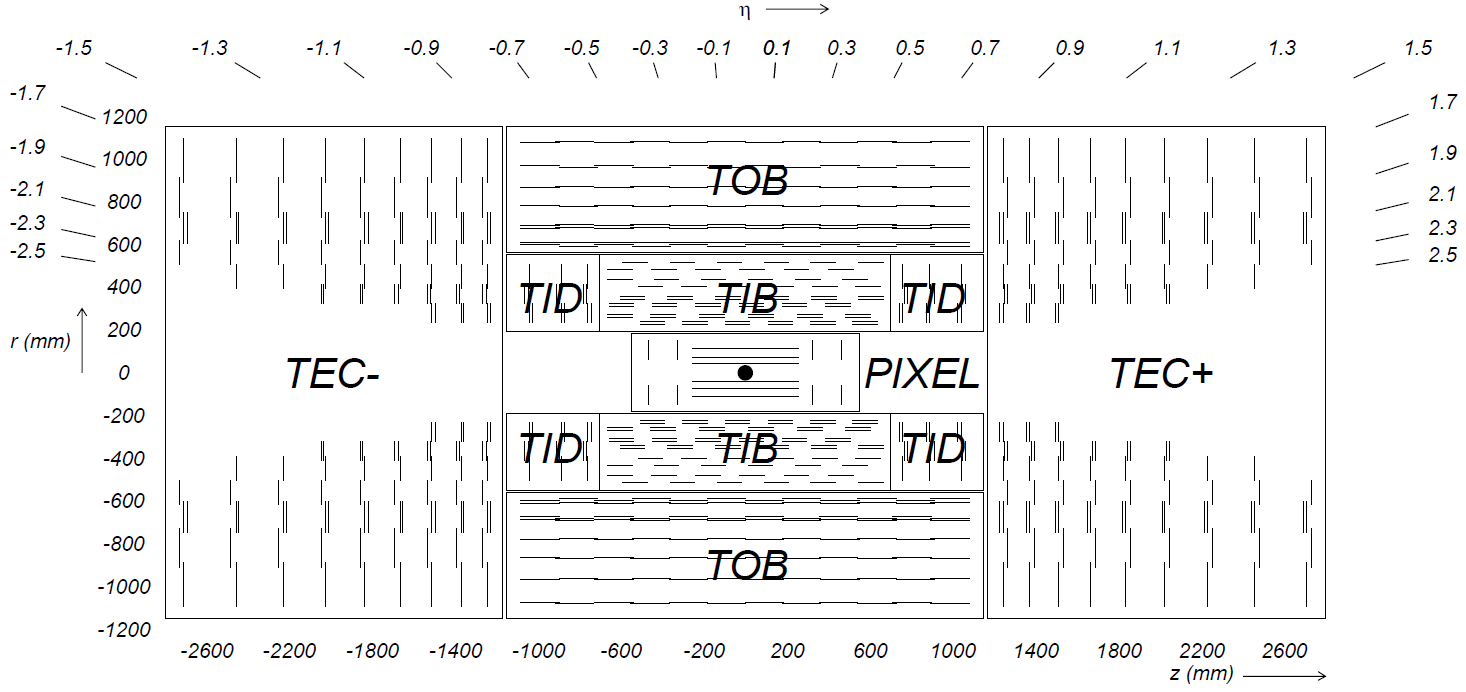
\includegraphics[width=0.95\textwidth]{images/TrackerWhole.png}
    \caption{The tracking system in \runone~\cite{1748-0221-3-08-S08004}}
    \label{fig:TrackerWhole}
\end{figure}

\textbf{Pixel tracker}\\

As the pixel detector is closest to the interaction vertex, it experiences the highest flux of particles at $\approx$ 1 MHz per mm$^{2}$. The fine granularity of the pixel detector (100 x 150 $\mu$ m in r-$\phi$ x z) is required in order to keep the occupancy below 1\%. It consists of three barrel layers which range between 4 cm and 10.2 cm from the interaction point and 2 disks which are transverse to be beamlines as seen in Fig.~\ref{fig:TrackerWhole}.\\

\textbf{Strip tracker}\\
Two types of silicon strip tracker are used. Closest to the interaction point (20 - 50 cm) are the tracker inner barrel detectors (TIB) which contain silicon micro-strips (10 cm x 80 $\mu$m). An occupancy of $\approx$ 2 - 3~\% is achieved for a fluence of $\approx$ 60 kHz per mm$^{2}$.
An increased strip pitch of 180$\mu$m can be used in the tracker outer barrel (TOB) due to the lower fluence of 3 kHz per mm$^{2}$. To cover the larger surface area, the strip length is increased to 25 cm. However increased strip length increases the noise. To combat this the strips are made thicker to 500$~\mu$m compared to 320$~\mu$m in the TIB.
The tracker inner disk (TID) and tracker end cap (TEC) have strips which are aligned radially to the beamline with a strip pitch of 80$~\mu$m and 200$~\mu$m, respectively. The TID and TEC extend the tracker acceptance to $\abs{\eta}<2.5$.

\subsection{Electromagnetic Calorimeter}

The electromagnetic calorimeter (ECAL) is a homogenous, hermetic detector made up of 61200 (7324) lead tungstate (PbWO$_{4}$) crystals in the barrel (endcap) region. In the barrel region the light from these scintillating crystals is collected in avalanche photodiodes and by vacuum phototriodes in the endcap region. The barrel region covers $\abs{\eta}<1.479$ whilst the two semi-circular `Dees' which make up the endcaps extend the range to $\abs{\eta}<3.0$. Good resolution can be obtained from PbW0$_{4}$ crystals as well as being fast and radiation resistant. The crystals have a high density so that the ECAL can be compact and importantly they are optically clear. The scintillation decay time is comparable to the time between bunch crossings with 80\% of light being emitted within 25ns. The crystals have a tapered shape in the barrel region and lie parallel in the endcap region. In the barrel the crystals have a length of 230 mm and the front faces have dimensions of 22 x 22 mm$^{2}$, whilst the rear faces measure 26 x 26 mm$^{2}$. The crystals are 1.29 m from the beam line in the barrel region and 3.15 m from the the interaction point in the longitudinal direction in the endcap region. The crystals are contained in thin-walled aluminium structures which make up submodules.

In the endcap region there is a preshower detector, seen in Fig.~\ref{fig:ecal}, which is a two-layer sampling calorimeter. There are two layers of lead used as a radiator material to initiate the electromagnetic shower and silicon strip detectors after each layer (orthogonal in each plane) to measure the energy depositied. The preshower detector helps to identify neutral pions and to distinguish electrons from minimum ionising particles.

\begin{figure}[ht!]
\centering
    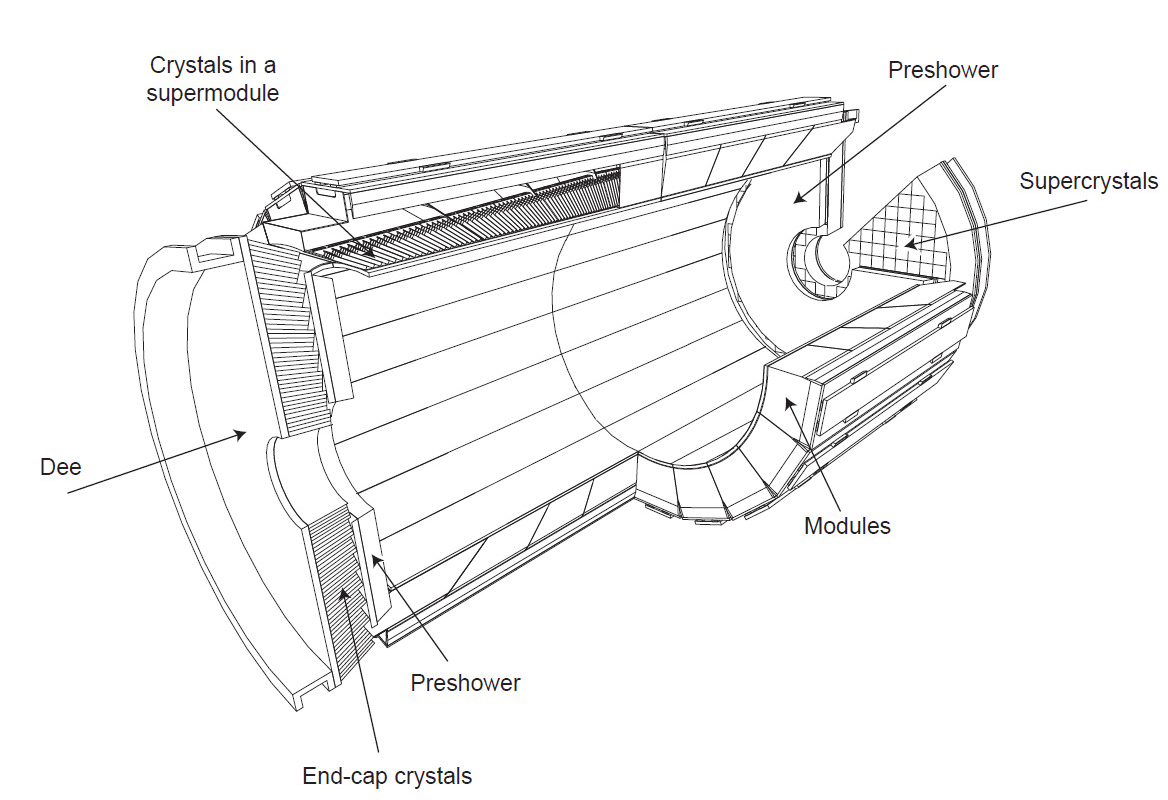
\includegraphics[width=0.95\textwidth]{images/ecal.png}
    \caption{The ECAL system where modules contain submodules and the 36 supermodules are made up of four modules each. The supercrystals are made up groups of 5 x 5 crystals in the endcap.}
    \label{fig:ecal}
\end{figure}

\subsection{Hadron Calorimeter}

The hadron calorimeter (HCAL) is used for identifying hadron jets. It has barrel (HB) and endcap (HE) regions made up of sampling calorimeters which have coverage of $\abs{\eta}<1.3$ and $1.3<\abs{\eta}<3.0$, respectively. The HB and HE are placed between the ECAL and solenoid magnet therefore are restricted to the radial dimensions, R, of 1.77 m $<$ R $<$ 2.95m. The barrel consists of two halves, HB+ and HB-, which are composed of 36 wedges made up of 14 flat brass absorber plates parallel to the beam axis, alternated with plastic scintillator. Stainless steel plates are used for the innermost and outermost plates to provide structural support. The HE has a similar system of alternating absorber and plastic scintillator.
Due to their restricted dimensions the HCAL and ECAL do not always contain all of the energy from the hadronic and electromagnetic showers, respectively. Therefore another detector known as the outer hadronic calorimeter (HO) is embedded in the muon system which lies outside of the solenoid magnet to measure the energy leakage from the HCAL and ECAL.
The forward HCAL extends the range from $\abs{\eta}<2.3$ to $\abs{\eta}<5.2$ to detect very forward jets. The hermeticity of the detector ensures a good converation on detecting the total hadronic energy and hence good resolution can be obtained on missing energy which could come from neutrinos or BSM particles.

\begin{figure}[ht!]
\centering
    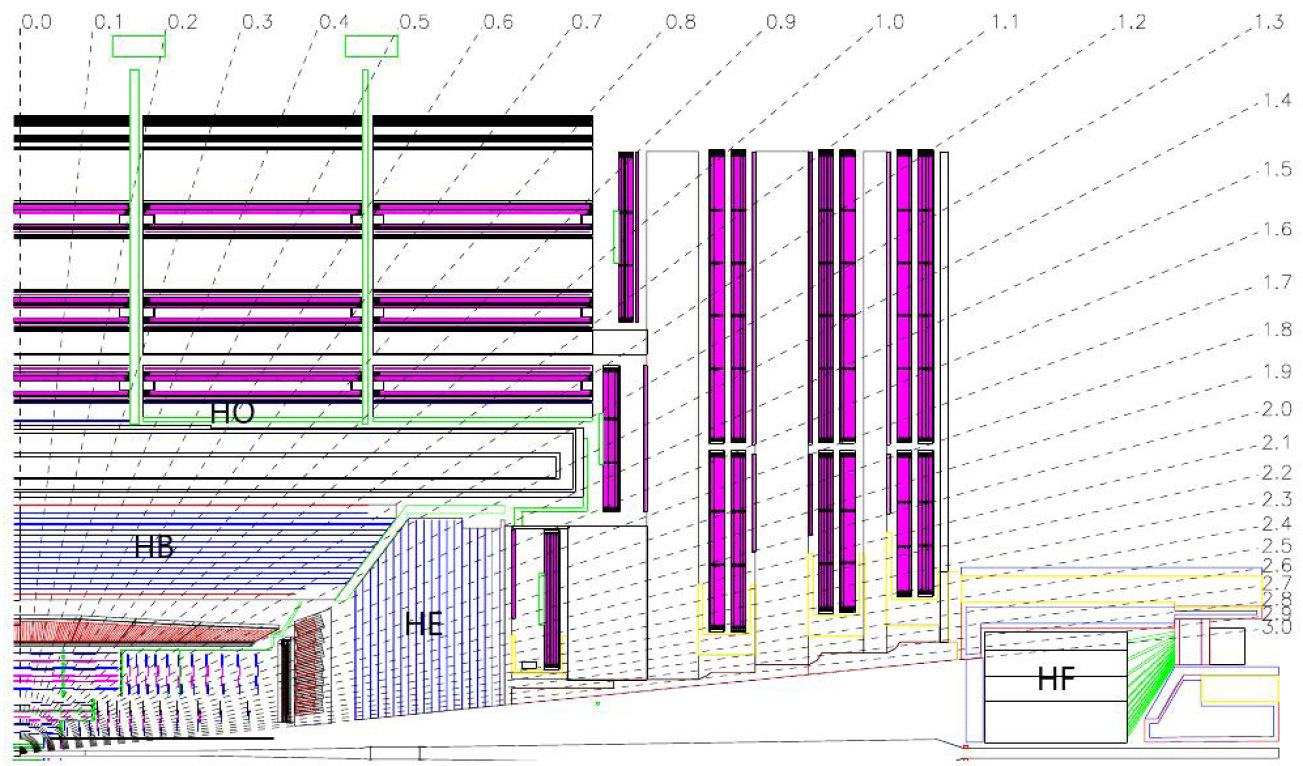
\includegraphics[width=0.95\textwidth]{images/HCAL.png}
    \caption{The HCAL system.}
    \label{fig:hcal}
\end{figure}

\subsection{Muon Chambers}

As the name CMS suggests, muon identification and measurement was a central focus in the design of the detector. The muon chambers are interspersed within the iron flux return yoke. These thick layers of iron act as a hadron absorber. Muons are much less affected by radiative losses through the tracker material than electrons, therefore they are able to penetrate through to the outermost layers of the detector. Figure~\ref{fig:muonchamber} shows the layout of the muon chambers around the detector. The muon chambers consist of a cylindrical barrel section and 2 planar endcaps. The magnetic field is uniform in the barrel region where drift tubes (DT) are arranged into chambers, some of which make measurements in r-$\phi$ and some of which make measurements in z. This provides a high efficiency for matching individual hits in different stations to one single muon track.
In the endcaps where the muon flux is high and the magnetic field is non-uniform, cathode strip chambers (CSC) are used due to their fine segmentation, fast response and radiation resistance. The CSC stations are aligned perpendicular to the beam line and are positioned between the flux return plates. The cathode strips are positioned as radial lines and the anode wires run perpendicalar to the cathode strips. Together they can measure the position in r-$\phi$ and $\eta$. The CSCs provide robust pattern recognition for matching hits to other stations and to the tracker as well as for rejecting non-muon backgrounds. 
Together the barrel and end-cap region provide uninterrupted coverage up to $|\eta|<2.4$.\\
Resistive plate chambers (RPC) are added in the barrel and endcap sections of the muon chambers. They consist of two parallel plate chambers which sandwich readout strips, known together as a double-gap module. The sum of the two signals from each gap creates one total induced signal. There are six RPCs in the barrel section and there are three layers of RPCs in the endcap.
 Where ambigious tracks exist due to multiple hits in the muon chambers, the RPCs can help to distinguid the correct track. They have a fast response and can time-tag an ionising event in much less than the 25 ns bunch spacing time and hence they can assign candidate tracks to the relevent bunch crossing. The resolution of the RPCs is courser than the DTs and CSCs and the information from the RPCs is used in the trigger which is described in the following section

\begin{figure}[ht!]
\centering
    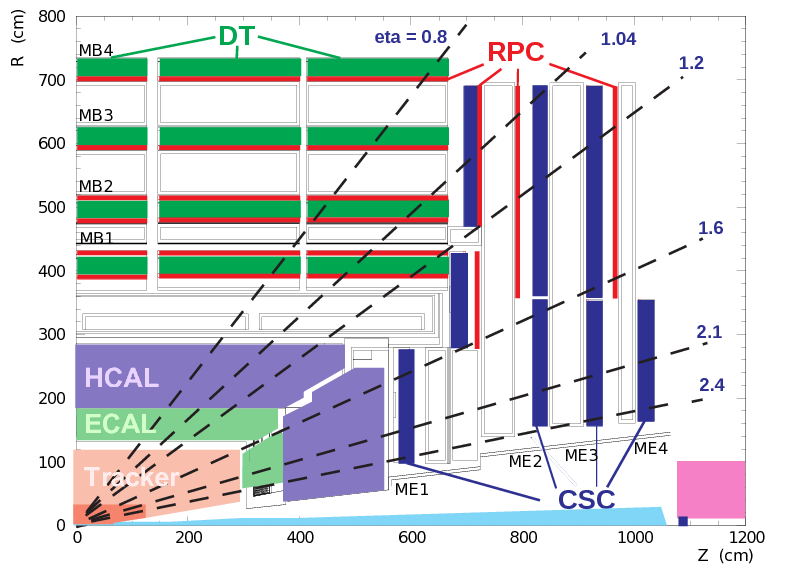
\includegraphics[width=0.95\textwidth]{images/MuonChambers.png}
    \caption{The muon chamber system ~\cite{Kim:2012ix}.}
    \label{fig:muonchamber}
\end{figure}

\subsection{Trigger \label{det:trigger}}
As each of the subdetectors have now been described, the remaining hardware and software which collects the information for analysis can now be discussed. The amount of information which can be stored is much less than the amount produced within the subdetectors. Collisions occur at a rate of 40 MHz (beam crossing interval of 25 ns) and the rate reduction capability of the trigger system was designed to reduce to rate by at least a factor of $10^6$. This occurs in two main stages, the Level-1 (L1) trigger and High-Level Trigger (HLT). The L1 trigger is the first stage and is composed of highly programmable custom electronics, mainly FPGAs. ASIC and programmable memory lookup tables are used where higher speed and radiation hardness is required closer to the beam spot as radiation exposure can create spikes in the signal. The high resolution data is held in the front-end electronics whilst the L1 trigger decides whether or not to keep the event based on courser information from the calorimeters and muon chambers. The HLT trigger is a software based filter farm ($\approx$ 1000 processers) which has access to all of the read-out data from the subdetectors. The HLT can assess more complex information in order to filter out uninteresting events and categorise interesting ones.
% \fixme{Tracking information is used in the high level trigger (HLT)}

\subsection{Upgrades for \runtwo}

In LS1, repairs were made to the LHC magnet splices to allow safe operation at the design energy of $\sqrt{s} = 14~\TeV$. All of the detectors on the LHC ring were able to make essential repairs and upgrades. For CMS this included repairing damaged silicon pixels and strips in the tracker and inserting the tracker back into CMS with better centering around the beam line. The temperature of the tracker was lowered to -20 degrees celcius to mitigate against radiation damage. In the ECAL the EE and ES subsystems underwent minor repairs. New photodetectors were added to the HO in the HCAL to improve the signal to noise ratio. The main change to the muon systems has been to the RPCS with the addition of the fourth disk (RE4). For the muon system CSCs, 72 chambers have been added to the existing 468 chambers. In addition to the detector upgrades, improvements have been made to the trigger and DAQ.

These upgrades have allowed CMS to operate at $\sqrt{s} = 13~\TeV$ in 2015 with the smaller bunch spacing of 25~ns compared to the previous 50~ns bunch spacing in \runone.

\subsection{Data collections used in this thesis}
Add section describing data used in this thesis, when collected, etc.

% Upgrade in energy and 50ns to 25ns bunch\\
% L1-Trigger system-higher granularity -additional processingcapabilities, 
% upgrade photo-detectors and electronics for the hadron calorimeters\\
% (HCAL) to reduce background signals - improve measurement of jets and missing-energy
% at high PU.
% Reference to pixel detector paper with upgrades~\cite{Dominguez:1481838}

% \begin{figure}[ht!]
% \centering
%     \includegraphics[width=0.55\textwidth]{images/TrackerUpgradeXSec.png}
%      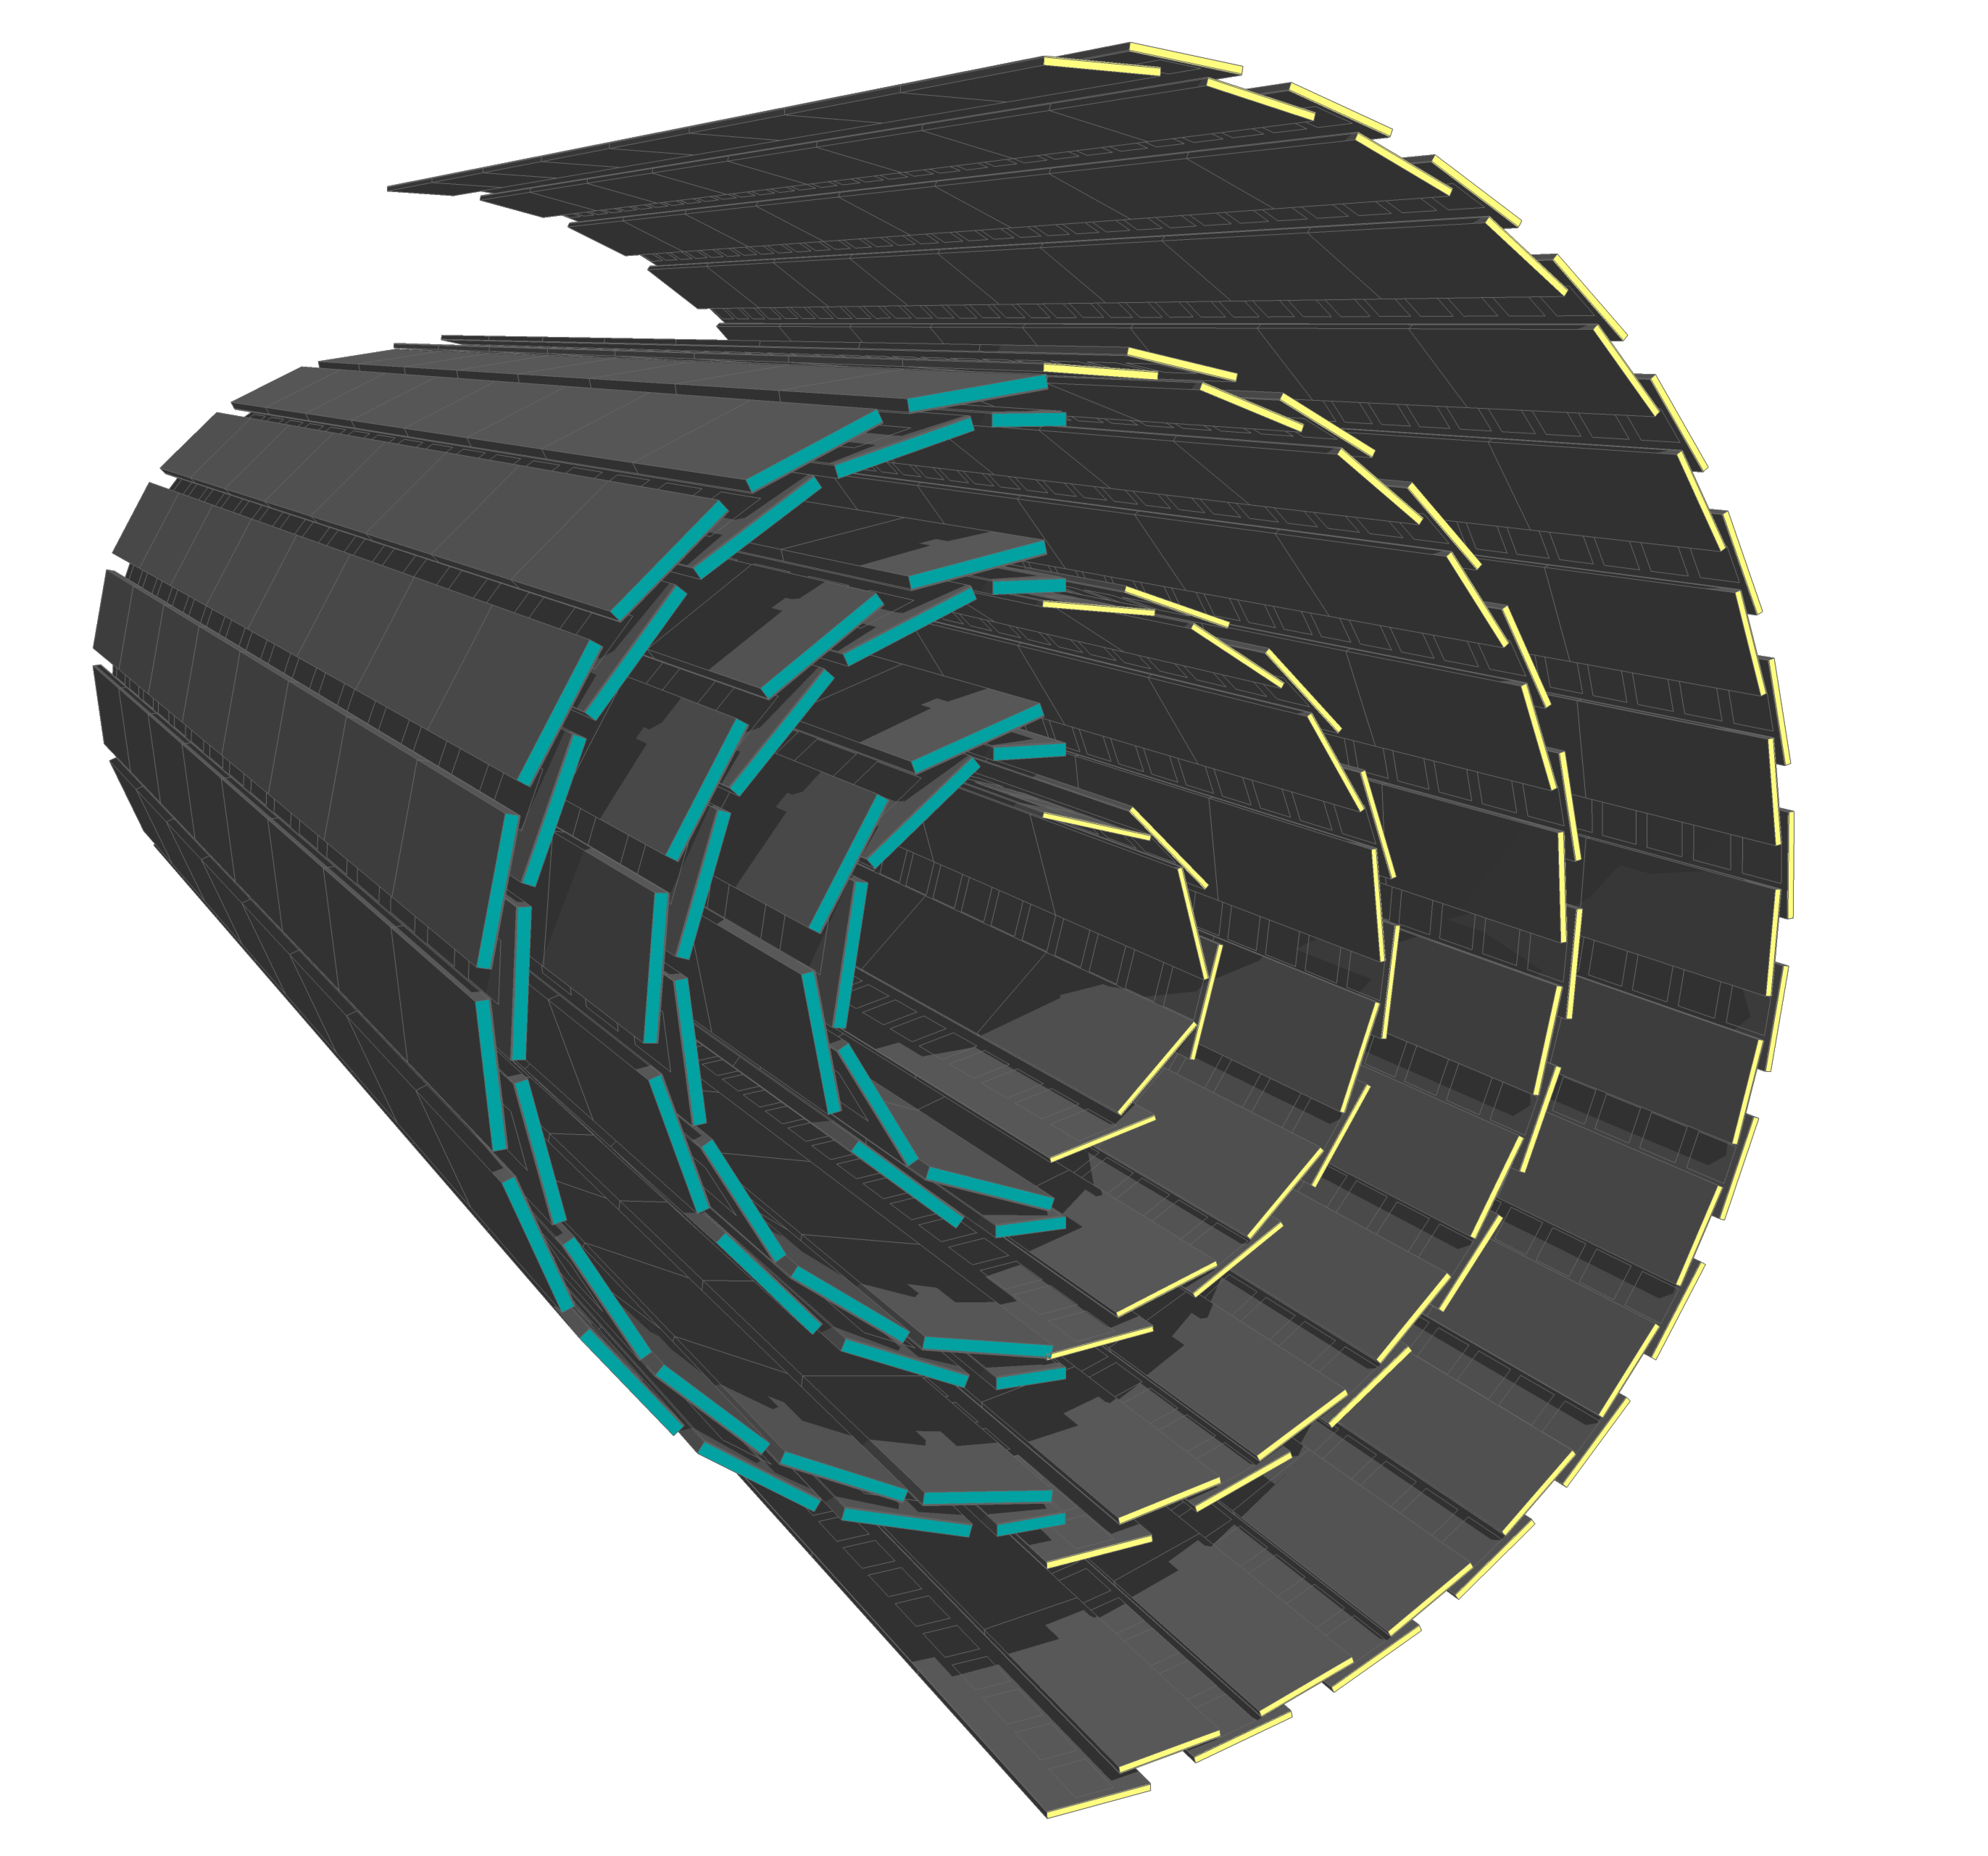
\includegraphics[width=0.42\textwidth]{images/TrackerUpgradeBarrel.png}          
%     \caption{Pixel tracker with half initial and half upgrade geometries~\cite{1742-6596-513-2-022032}}
%     \label{fig:pixel}
% \end{figure}



% \addcontentsline{toc}{chapter}{Detector}
\chapter{Event Reconstruction}
\label{c:recon}
% In this chapter the software and algorithms used to reconstruct particle physics objects are detailed. The idea is to work backwards from the information obtained from each of the sub-detectors to determine what particles passed through them.\\
% A software framework known as CMSSW has been developed in order to reconstruct the read out from the detector for each event


In Chapter~\ref{c:det}, each of the sub-detectors in CMS have been described; how particles interact with them and how electrical signals are read out. The next step is to combine the readouts from each detector in order to reconstruct the resulting particles from an interesting proton-proton collision. This snapshot of the collision output is known as an \emph{event}. An event will also contain PU from reconstructed particles from other simultaneous uninteresting collisions from the same bunch crossing. Algorithms are used in order to subtract PU particles from the stored event. 
As a particle will usually traverse more than one sub-detector, it is advantageous to combine these outputs in order to reconstruct and identify the particle. This is achieved using the \emph{particle-flow} (PF) algorithm described in Section~\ref{sec:PF}. The objects which can be reconstructed using the PF algorithm such as muons, electrons, and jets are discussed in Sections~\ref{sec:muonreco},~\ref{sec:electronreco},~\ref{sec:jetreco} respectively. Further information can be obtained from these reconstructed objects such as how likely a jet is to have originated from a b-quark (Section~\ref{sec:btagreco}) and how the presence of neutrinos can be inferred by the imbalance of energy in the transverse plane of the detector (Section~\ref{sec:METreco}).  
The information from the detector is processed using a distributed computing infrastructure with custom software made by CMS, CMSSW.
% This chapter will discuss the main software used to reconstruct events from the detector read-out, CMSSW, and how a worldwide computer farm is used to process data.


% \section{Software}

% To-do:
% CMSSW, grid

\section{Track reconstruction}

Approximately 1000 charged particles are expected to traverse the CMS tracker at each bunch crossing at a PU of $\approx 20$ concurrent collisions. Each particle will interact with the silicon tracker as it continues through its trajectory from the collision point. Algorithms are designed to match hits in tracker along each particle's trajectory in order to reconstruct its path so information about the charge and momentum of the particle can be obtained. Not only is the tracker information used in offline reconstruction but it is used in the HLT, therefore it must have a fast response. Reconstructed paths from random particle hits in the tracker are considered to be \emph{fake tracks}~\cite{1748-0221-9-10-P10009}.\\
Knowledge of particle trajectories can help to pinpoint the collision vertex also known as the \emph{primary vertex} and described further in Section~\ref{sec:PVreco}. Accuracy in reconstructing tracks is essential for b-tagging as described in Section~\ref{sec:btagreco}.
Electrons lose energy through the tracker material in a non-gaussian way such that their tracks can not be fitted using the standard Kalman Filter. A Gaussian-Sum-Filter refit~\cite{GSF_Electron_Reconstruction_CMS}, which uses a sum of gaussians to estimate the energy loss, takes into account the interaction of electrons through the tracker material.


\section{Primary vertices \label{sec:PVreco}}

Primary vertices are the point at which the collision occurred, as opposed to secondary vertices which originate at the decay of subsequent particles coming from the collision. The first step in reconstructing primary vertices is to consider tracks which are consistent with the beam spot and cluster them into candidate vertices, separated along the z direction. Next a 3D fit is made and candidates which are compatible with originating from the beamline are kept. Primary vertices are ranked according to the sum of the momentum squared of all the tracks considered to have originated from that vertex. The vertex with the largest sum is regarded as the signal vertex, ie. the event with higher momentum objects which is most likely to have fired the trigger. 

\section{Particle-flow algorithm ~\label{sec:PF}}

The particle-flow (PF) algorithm combines information from all sub-detectors described in Section~\ref{c:det}, in order to improve the reconstruction of `final state' particles such as electrons, muons, photons, neutral hadrons and charged hadrons. From this information more complicated higher-level objects, such as jets, can be reconstructed as described in the subsequent sections. Collections of different sub-detector objects, such as tracks or ECAL/HCAL hits, are created and each object is subsequently removed from each collection as they are identified as belonging to a final state particle within the algorithm.\\
The particle-flow algorithm reconstructs objects in an order starting from the easiest to reconstruct unambiguously. The hardest objects to reconstruct such as neutral hadrons are one of the last to be reconstructed because their properties can be constrained from the previously reconstructed objects.
The first objects to be reconstructed are PF muons. Each muon identified from the muon chambers is associated to compatible hits in the tracker. This associated track is then removed from its collection. Next, a Gaussian-Sum-filter refit is used to extrapolate electron candidate trajectories to the ECAL. On average, electrons have shorter trajectories than muons due to losing much of their energy through interactions with the tracker material. Tracker and ECAL variables are combined for the final identification of a PF electron after which the track and ECAL clusters are removed from their respective collections.\\
Charged hadrons are reconstructed from the remaining tracker, ECAL and HCAL deposits where the calorimeter hits are compatible with the tracker hits. Again, these hits are removed from the respective collections. Neutral hadrons leave no tracks in the tracker but have deposits in the ECAL and HCAL. Photons leave deposits in the ECAL but not the HCAL.\\


\section{Isolation \label{sec:isolation}}

Relative isolation (RelIso), is a measure of how isolated the muons or electrons are from surrounding hits in the detector from charged hadrons, neutral hadrons and photon energy which could contribute to a mis-measurement of their momentum. Only charged hadrons which are consistent with the signal primary vertex are considered in the calculation. As it is not possible to determine whether neutral hadrons are consistent with the signal primary vertex we can use the fact that the ratio of neutral to charged energy has been measured to be $\approx 0.5$. Hence the neutral hadronic energy in the transverse plane of the detector coming from the primary vertex, $E_{T,PV}^{NH}$, can be calculated as seen in Eq.~\ref{eqn:neutralE}, where $E_{T,sub}^{CH}$ is the transverse energy from charged hadrons which are associated to a sub-leading primary vertex and $E_{T,Tot}^{NH}$ is the total transverse neutral hadronic energy. 
% This is called the \emph{delta Beta correction}.
 The max() function ensures that the corrected neutral hadronic energy is never defined as negative.


\begin{centering}
\begin{equation}
\Sigma E_{T,PV}^{NH}  =  max(0, \Sigma E_{T,Tot}^{NH} - 0.5*\Sigma E_{T,sub}^{CH})
\label{eqn:neutralE}
\end{equation}
\end{centering}



The RelIso formula, with the correction to neutral hadronic energy, can be found in Eq.~\ref{eqn:dBRelIso}. It is defined in a cone of radius $\textrm{R}=0.4$ and scaled by $1\; / \;\pt^{\mu}$ (where \pt is the momentum in the transverse plane of the detector) so that lower momentum muons are required to have less energy from hadrons and photons in the cone to be considered isolated.

\begin{centering}
\begin{equation}
RelIso = \left( \Sigma E_{T}^{CH} + \Sigma E_{T,PV}^{NH} +  \Sigma E_{T}^{\gamma} \right) \; / \;   \pt^{\mu}
\label{eqn:dBRelIso}
\end{equation}
\end{centering}


Equation~\ref{eqn:dBRelIso} is used to define relative isolation for muons; for electrons it is similarly defined, however, the neutral hadronic energy is estimated using a different method. The relative isolation for electrons is defined in Eq.~\ref{eqn:rhoCorr} where EA denotes Effective Area. The EA is calculated from the average PU energy density per unit area in the $\rho$ ($\rho=\phi-\eta$) plane and the effective area based on shower shapes that has been measured by CMS (which depends on the $\eta$ value in the supercluster) for each event.

% \begin{centering}
% \begin{equation}
% C^{\rho} = \left( \Sigma E_{T}^{NH} + \Sigma E_{T}^{\gamma} - \rho\times\textrm{EA} \right) 
% \label{eqn:rhoCorr}
% \end{equation}
% \end{centering}

Equation~\ref{eqn:eRelIso} gives the RelIso formula for electrons with neutral hadronic energy correction where $\rho$ stands for the median density of pile-up contamination.

\begin{centering}
\begin{equation}
RelIso = \left( \Sigma E_{T}^{CH} + \Sigma E_{T}^{NH} + \Sigma E_{T}^{\gamma} - (\rho\times\textrm{EA}) \right) \; / \;   \pt^{e}
\label{eqn:eRelIso}
\end{equation}
\end{centering}

% \begin{centering}
% \begin{equation}
% RelIso = \left( \Sigma E_{T}^{CH} + C^{\rho} \right) \; / \;   \pt^{e}
% \label{eqn:eRelIso}
% \end{equation}
% \end{centering}

\section{Muons \label{sec:muonreco}}

It is important to be able to identify isolated muons coming from the signal process rather than from further decays from within jets or from mismatched tracks. Applying the identification criteria in Table~\ref{tab:muon_tight_cuts} can help to ensure a high purity of real muons are selected from the PF candidates described in Section~\ref{sec:PF}. Two working points (WP) are defined, tight and loose. Tight muons have tighter requirements on various quantities including \pt, as lower momentum muons are harder to distinguish from other particles. Tight muons are used when making selection requirements on how many muons should be in the event from the signal process. Loose muons are used to veto additional objects which are still likely to be muons but could be misidentified object such as pions. The loose criteria will capture more real muons in its selection but with a lower purity.
% but this is necessary when requiring a maximum number of muons in the event. 
The cut values for each working point are given in Table~\ref{tab:muon_tight_cuts} for the 8 TeV analysis, which is in Section~\ref{c:Run1}, and the 13 TeV analysis, which is in Section~\ref{c:Run2}.

The transverse impact parameter in the $\phi$-plane with respect to the leading primary vertex is denoted as d0 in the table. The distance between the leading primary vertex and the muon track in the z-direction is denoted dz. These two variable can be used to establish how consistent the muon track is with the leading primary vertex.
A \emph{Global Muon} is a muon which has been identified from both hits in the muon chamber and hits in the tracker whereas a \emph{Tracker Muon} has only been identified from tracker hits.


\begin{table}[htpb!]
\footnotesize
\begin{center}
\begin{tabular}{|r|c|c|c|c|}
\hline
\multicolumn{1}{|l|}{}                                          & \multicolumn{2}{c|}{Tight WP} & \multicolumn{2}{c|}{Loose WP} \\ \cline{2-5} 
Requirements                                                    & 8 TeV         & 13 TeV        & 8 TeV         & 13 TeV        \\ \hline
Is a Global Muon and a Tracker Muon                               & yes           & yes           & yes           & yes           \\
\pt (\GeV)                                                     & $>$30            &$>$ 26            & $>$10            &$>$ 10            \\
$\lvert \eta \rvert$                                          &  $<$2.1           &  $<$2.1           &  $<$2.5           &  $<$2.5           \\
RelIso                                                    &  $<$ 0.12          & $<$  0.15          & $<$  0.2           &  $<$ 0.25          \\
Number of valid hits in the tracker                          & $>$5             & $>$5             & -             & -             \\
Number of hits in the muon stations                          & $>$0             & $>$0             & -             & -             \\
d0 (cm)  & $<$0.2           & $<$0.2           & -             & -             \\
dz (cm)       & $<$ 0.5           & $<$ 0.5           & -             & -             \\
Number of pixel hits                                         & $>$0             & $>$0             & -             & -             \\
Normalised $\chi^{2}$ of track                              & $<$ 10            &$<$  10            & -             & -             \\
Number of matched muon stations                             &  $>$1             &  $>$1             & -             & -             \\ \hline
\end{tabular}
\caption{The cuts used for the tight and loose muon identification at 8 TeV~\cite{muonIDtwikieight} and 13 TeV~\cite{muonSFtwiki}}
\label{tab:muon_tight_cuts}
\end{center}
\end{table}



\section{Electrons \label{sec:electronreco}}

Electrons lose a lot of energy in the tracker material via Bremsstrahlung. This is one of the biggest challenges in reconstructing electrons as this radiation needs to be taken into account to accurately measure their momentum. These Bremsstrahlung photons can also convert into electron-positron pairs in the tracker material creating secondary electrons which must be distinguished from the signal electrons coming from the hard process. In this thesis the word electron is mostly used to include both charges, electron and positron. 

As with Section~\ref{sec:muonreco} for muon reconstruction, two working points are defined for electrons from the PF candidates. Tight electrons are used when requiring electrons as part of the signal process and a looser set of criteria are used in order to veto on extra electrons in the event to have a strict selection. The loose selection will of course contain more electrons but with a lower purity. 

There are multiple ways to identify electrons, two of which are used in this thesis. At 8 TeV a multivariate technique to identify electrons was used. At 13 TeV a \emph{cuts based identification} was used as the electron tools from CMS were not as advanced by the time the analysis was performed.

The tight and veto working points at $\sqrt{s}=8$ TeV can be found in Table~\ref{tab:electron_tight_cuts8}. The multivariate algorithm used for electron identification assigns a discriminator value which is closer to one for candidate particles which are more consistent with being a real electron and closer to zero if not. A conversion veto is applied for tight electrons which mitigates against identifying electrons which have come from photons converting into an electron-positron pair in the detector~\cite{Khachatryan:2015hwa}.


\begin{table}[htpb!]
\footnotesize
\begin{center}
\begin{tabular}{|r|c|c|}
\hline
Requirements   & Tight & Veto \\ \hline
\ET  GeV & $>$30    & $>$20   \\
$|\eta| $  & $<$2.5   & $<$2.5  \\
$|$d$0|$ & $<$0.02  & -    \\
ConversionVeto & yes   & -    \\
MVA ID & $>$  0.9   &$>$   0    \\
RelIso   & $<$0.1   & $<$0.2  \\ \hline
\end{tabular}
\caption{The cuts used for the tight and veto electron identification at $\sqrt{s}=8$~TeV~\cite{electronIDeight}}
\label{tab:electron_tight_cuts8}
\end{center}
\end{table}

The tight and veto working points are given for the barrel and endcap in Table~\ref{tab:electron_tight_cuts13} for the $\sqrt{s}=13$~TeV analysis. 

\begin{table}[htpb!]
\footnotesize
\begin{center}
\begin{tabular}{|r|c|c|c|c|}
\hline
& \multicolumn{2}{c|}{Tight} & \multicolumn{2}{c|}{Veto} \\
\cline{2-5}
%&Tight & TIght & Veto & Veto \\
Requirements &  Barrel        &   Endcap  &  Barrel        &   Endcap  \\
%&  ($|\eta_{SuCluster}|< 1.4442$)         &   ($1.5660<|\eta_{SuCluster}|<2.5$)  &  ($|\eta_{SuCluster}|< 1.4442$)         &   ($1.5660<|\eta_{SuCluster}|<2.5$)  \\
\hline
full $5\times5 \; \sigma_{I_{\eta}I_{\eta}} $ & $ <$0.0101 & $ <$0.0279 & $ <$0.0114 & $ <$0.0352\\
$|\Delta \eta_{In}| $  & $ <$0.00926 &$ <$ 0.00724  & $ <$0.0152 & $ <$0.0113  \\
$|\Delta \phi_{In}|  $  &  $<$0.0336 & $<$0.0918 & $<$ 0.216 & $<$0.237  \\
$\frac{h}{E} $ &$<$0.0597 & $<$0.0615  &$<$0.181 & $<$0.116  \\
RelIso & $\leq$0.0354 & $\leq$0.0646& $\leq$0.126 & $\leq$0.144\\
$\frac{1}{E} - \frac{1}{p}  $ & $<$ 0.012 & $<$ 0.00999  & $<$ 0.207 & $<$ 0.174 \\
$|$d$0| < $  & $<$0.0111 & $<$0.0351  & $<$0.0564 & $<$0.222\\
$|$dz$| $  & $<$0.0466 & $<$0.417 & $<$0.472 & $<$0.921\\
expected missing inner hits  & $\leq$2 & $\leq$1 & $\leq$2 & $\leq$3  \\
pass conversion veto & yes & yes& yes & yes  \\
\hline
\end{tabular}
\caption{The cuts used for the tight and veto electron identification at $\sqrt{s}=13$~TeV~\cite{electronID} where barrel is $|\eta_{SuCluster}|< 1.4442$ and endcap is  ($1.5660<|\eta_{SuCluster}|<2.5$)}
\label{tab:electron_tight_cuts13}
\end{center}
\end{table}

Electron reconstruction can not be performed accurately in the transition region ($TR$) between the ECAL barrel and endcap, $1.4442<TR<1.5660$ and hence they are excluded from physics analyses.

\section{Jets \label{sec:jetreco}}
When partons such as quarks and gluons fragment and hadronise, into charged and neutral hadrons, they form showers of particles in approximately the same direction of travel as the original parton. These final state particles can be clustered into what is known as a \emph{jet} using the anti-$\kappa_{\textrm{T}}$ reconstruction algorithm~\cite{Cacciari:2008gp}. This is an infrared and collinear safe algorithm which starts with a high \pt `seed' hit in the calorimeter and uses the distance measure in Eq.~\ref{eqn:antikt1} to find the nearest hit to merge with. If the distance from the beam, $d_{iB}$ in Eq.~\ref{eqn:antikt2}, is smaller than the distance to another hit, $d_{ij}$, the particle is merged with the beam~\cite{Salam2010}. In this thesis, a distance parameter of $R = 0.5~\left(0.4\right)$ is used to reconstruct jets in the \runone (\runtwo) analysis in Chapter~\ref{c:Run1}~(\ref{c:Run2}). The distance parameter was changed for \runtwo to be consistent with the ATLAS experiment and to mitigate against PU contamination. 


\begin{equation}
d_{ij}=min\left( p_{\textrm{T}i}^{~-2},p_{\textrm{T}j}^{~-2} \right) \frac{\Delta R_{ij}^{2}}{R^{2}} \textrm{ , where } \Delta R_{ij}^{2} = {\left( y_{i} - y_{j}\right)}^{2} +  {\left( {\phi}_{i} - {\phi}_{j}\right)}^{2}
\label{eqn:antikt1}
\end{equation}

\begin{equation}
d_{iB}=p_{\textrm{T}i}^{2}
\label{eqn:antikt2}
\end{equation}

Corrections are applied to the jet energy to account for the non-uniform response of the detector in \pt and $\eta$. The first correction is the \emph{L1FastJet} correction which is applied to both data and simulation to remove the energy coming from PU events. The \emph{L2Relative} and \emph{L3Absolute} corrections respectively correct for the non-uniform response in $\eta$ and \pt for both data and simulation. The \emph{L2L3Residual} corrections are applied to simulation only and correct the remaining small differences in jet response between data and simulation such as correcting the jet absolute scale (JES). The jet energy resolution (JER) is also smeared by 10$\%$ as the resolution is worse in data than in simulation. Together these corrections are called the \emph{jet energy corrections}~(JEC)~\cite{Khachatryan:2016kdb}.
Jet identification critera are applied to suppress fake jets arising from electrons showering in the ECAL due to Bremsstrahlung. This includes requiring $|\eta|<2.5$, \pt$<30$~GeV and a separation from the nearest loose muon or electron of $\Delta R>0.4$.

The biggest gains in using the PF algorithm come from performing the jet reconstruction on PF particles. The jet-matching efficiency, jet energy resolution and the reconstruction of the jet \pt are improved compared to using calorimeter information alone~\cite{CMS-PAS-PFT-10-001}. 

\section{b-tagging ~\label{sec:btagreco}}
Reconstructing jets gives us the knowledge that the particles emerging from the collision include quarks and gluons. Being able to identify which flavour of quark hadronised in the detector is extremely useful for a wide range of analyses. Particularly for searches for final states containing four top quarks, the ability to identify b-quarks originating from the decay of top quarks is incredibly beneficial in allowing us to discriminate between the signal and backgrounds. 

The particle shower coming from the hadronisation of b-quarks will contain B mesons and $\Lambda_{B}$ baryons which travel further in the detector due to having longer decay times than light flavour (u, d, s) mesons resulting in a typical flight distance of up to a few centimetres~\cite{Collaboration2015BS0}. The \emph{impact parameter} (IP), defined as the distance between the primary vertex and the extrapolated point of closest approach of a track, will be larger for tracks coming from the decay of a hadron containing a b-quark. The tracks emerging from this decay can form a secondary vertex. This information is exploited in the Combined Secondary Vertex (CSV) algorithm~\cite{Chatrchyan:2012jua}. The CSV algorithm is used to identify or \emph{tag} jets which originate from b-quarks by assigning a discriminator value between 0 and 1, where larger values are more consistent with b-quark jets. Loose (CSVL), medium (CSVM) and tight (CSVT) working points are defined at values of the discriminator for a given mis-identification rate. For analyses at $\sqrt{s} = 13$~TeV the algorithm was improved and is called Combined Secondary Vertex version 2 algorithm (CSVv2)~\cite{CMS-PAS-BTV-15-001}. Working points, selection efficiencies for b-quarks and mis-identification rates are given in Table~\ref{tab:btag} 

\begin{figure}[ht!]
\begin{center}
    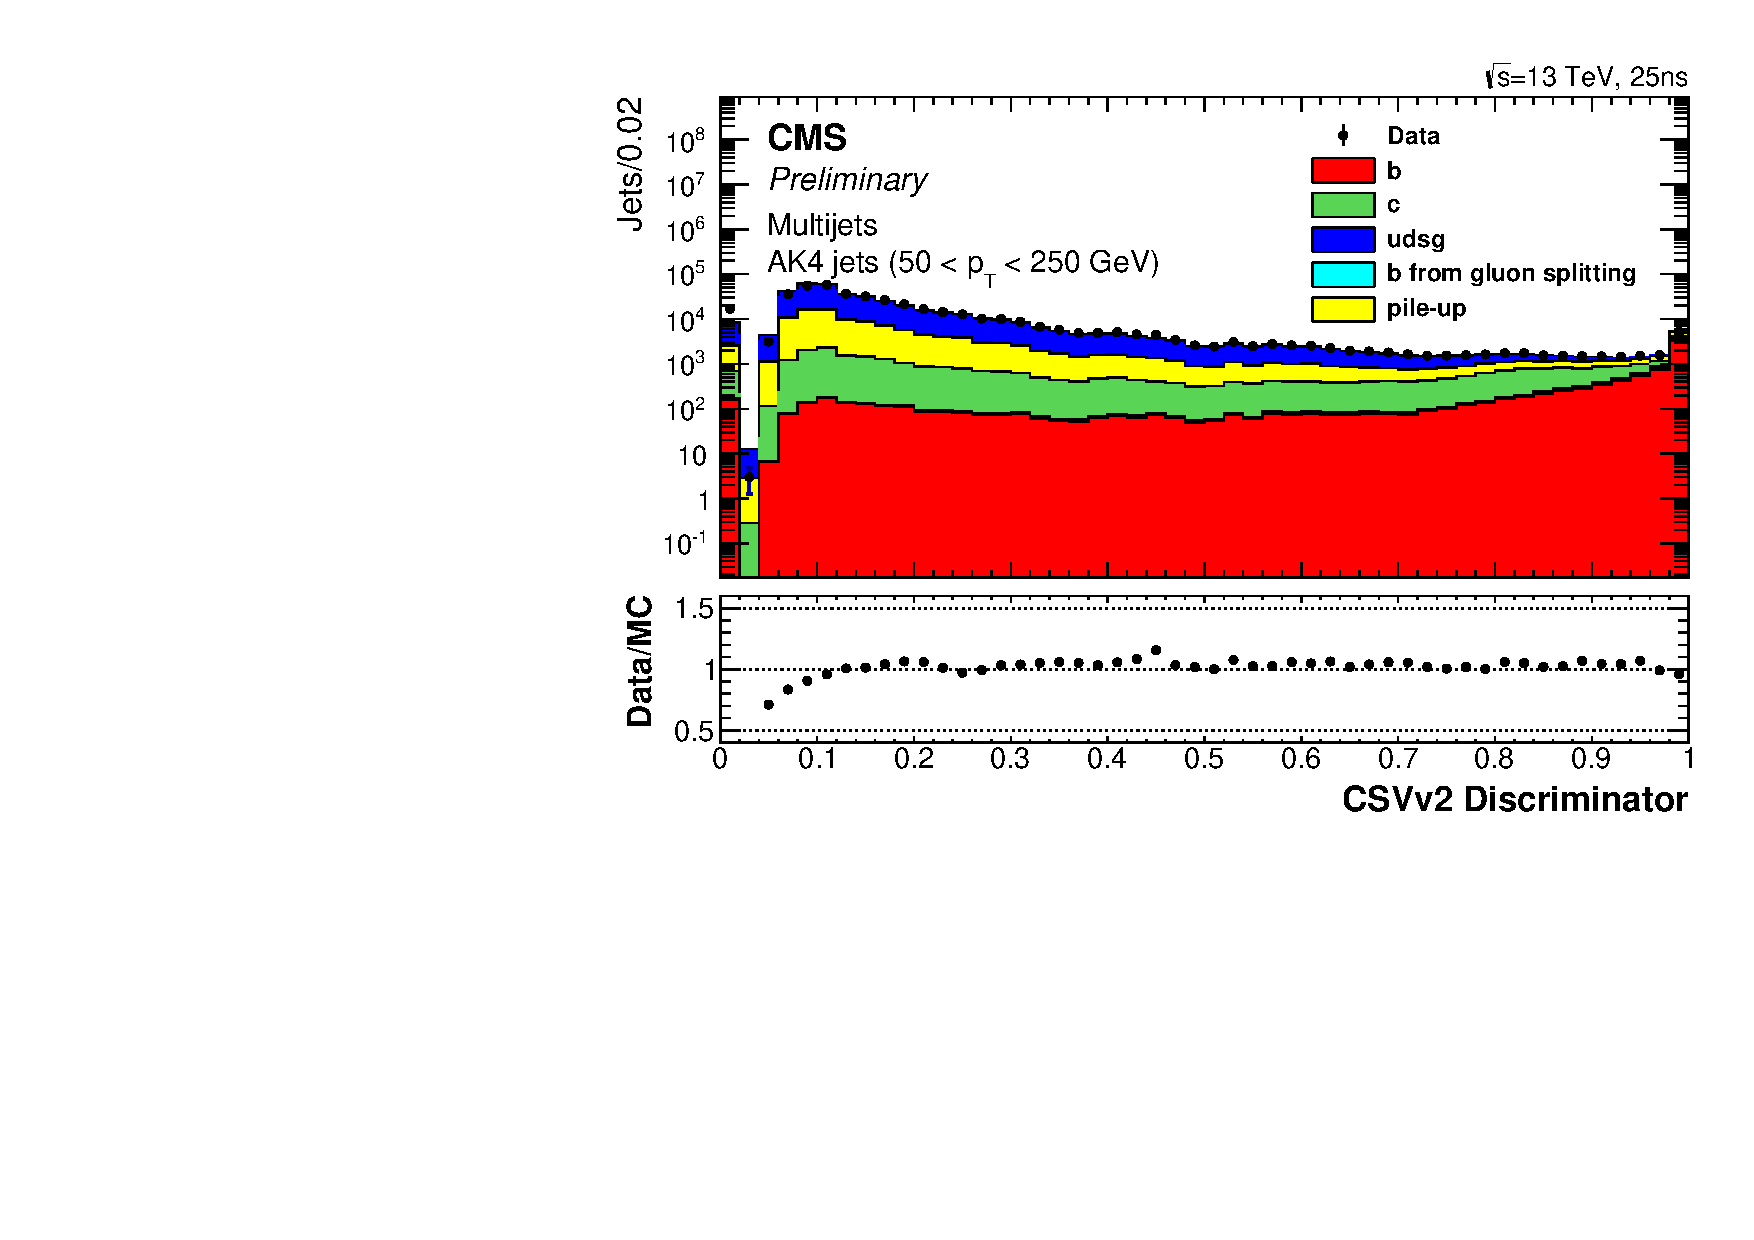
\includegraphics[width=0.99\textwidth]{images/btagCSV.pdf}
    \caption{CSVv2 discriminator distribution at $\sqrt{s}=13$~TeV using a multi-jets sample. Jets are reconstructed using the \antikt algorithm with $R=0.4$~\cite{CMS-PAS-BTV-15-001}.}
    \label{fig:CMSstairway}
\end{center}
\end{figure}
% \footnote{This efficiency was measured using the TTJets MLM sample for the medium working point at $\sqrt{13}$ TeV. The CSVv2L and CSVv2T efficiences have been taken from here~\cite{btageff} }.

\begin{table}[htpb!]
\footnotesize
\begin{center}
\begin{tabular}{l|l|c|c|c}
$\sqrt{s}$ (TeV)    & Name   & \multicolumn{1}{l|}{WorkingPoint} & \multicolumn{1}{l|}{Selection Efficiency ($\%$)} & \multicolumn{1}{l}{Mis-identification ($\%$)} \\ \hline
\multirow{3}{*}{8}  & CSVL   & 0.244                             & $<$80                                                 & 0.1                                               \\ \cline{2-5} 
                    & CSVM   & 0.679                             & $<$62                                                 & 0.01                                   \\ \cline{2-5} 
                    & CSVT   & 0.898                             & $<$35                                               & 0.001                                               \\ \hline
\multirow{3}{*}{13} & CSVv2L & 0.46                              & 82                                               & 11.5                                          \\ \cline{2-5} 
                    & CSVv2M & 0.8                               & 67                                               & 1.4                                           \\ \cline{2-5} 
                    & CSVv2T & 0.935                             & 47                                               & 0.15                                         
\end{tabular}
\caption{b-tagging working points and their selection and mistagging efficiencies}
\label{tab:btag}
\end{center}
\end{table}


\section{Missing transverse energy ~\label{sec:METreco}}
As it is not possible to detect neutrinos and potentially some BSM particles because they interact so weakly with matter, we can infer their existence by examining the sum of the momentum of particles in the transverse plane of the detector, where the transverse plane is defined to be transverse to the beamline. We start with the assumption that the total momentum in the transverse plane is zero. An imbalance in the sum of the momentum of detectable particles is considered to be missing transverse energy (\ETmiss), as defined in Eq.~\ref{eqn:MET}, where the \pt of jets is used after the JEC have been applied~\cite{CMS:2016ljj}.
\begin{equation}
\ETmiss = ~- \sum_{\textrm{all particles,}i} \hat{ {p}_{\textrm{T},i} }
\label{eqn:MET}
\end{equation}

\chapter{Simulation}
Particle physics events are simulated using Monte Carlo (MC) simulation so that they can be compared to the data. There are four main stages; generation (GEN), simulation (SIM), digitisation (DIGI) and reconstruction (RECO). The GEN stage consists of producing the hard scattering between the partons from the protons and the outgoing particles. The SIM stage continues from the GEN stage simulating the paths of the outgoing particles through the detector after which the response of the detector is generated in the DIGI step. The RECO stage then uses the algorithms discussed in this chapter to produce collections of high-level physics objects that are the same as what would be reconstructed in the detector from real data events.

\section{MC simulation Event Generators}

Event generators are used to simulate the signal and background processes at GEN-level. Using the proton PDFS and calculations of the Matrix Element (ME) associated to the Feynman diagrams for a particular process, a proton-proton collision can be replicated in simulation so that theory can be compared to experimental results. The main event generators used in the thesis are as follows:

\subsection{\MADGRAPH}
\MADGRAPH is a leading-order (LO) event generator~\cite{Alwall2011} which calculates the ME at tree-level with up to three additional partons. It takes as input PDF sets, for example NNPDF3.0 as shown in Fig.~\ref{fig:protonPDF}, which describes the kinematics of the incoming partons from the proton. The number and type of partons and the kinematics of the event are generated.
\subsection{\aMCATNLO}
The \aMCATNLO package~\cite{Degrande:2014sta} can simulate events at next-to-leading order (NLO) as it uses both tree-level and one-loop perturbations. These additional corrections from higher-order Feynman diagrams make the simulation more accurate than it's LO counterparts. This package include initial and final state radiation. Initial state radiation (ISR) refers to any particle which is radiated off of an incoming particle to the collision whereas final state radiation (FSR) refers to a particle radiated off the final state outgoing products of a collision.\\
\subsubsection{Negative event weights}
By including higher order perturbations to the cross section calculated in \aMCATNLO, it is necessary to consider terms which interfere destructively. This is achieved by assigning negative weights to some events within the generator so that the differential cross section is simulated correctly. The effective number of events, $N_{eff}$, produced by the generator corresponds to $events^{pos} - events^{neg}$ (this equates to the number of events that would be produced for the given cross section) whereas the total number of events produced correspond to $events^{pos} + events^{neg}$. Therefore these samples can be scaled using the negative event weight, $W_{events}^{neg}$, according to Eq. (\ref{eqn:negativeScaling}).

\begin{equation}
\label{eqn:negativeScaling}
W_{events}^{neg} = \frac{events^{pos} + events^{neg}}{events^{pos} - events^{neg}} = \frac{events^{Total}}{ events^{Total} - 2events^{neg}}
\end{equation}


\subsection{\POWHEG}
The `Positive Weight Hardest Emission Generator', known as \POWHEG~\cite{POWHEG}, has the advantage that it is a NLO generator which only produces positive weight events due to the fact that it generates the hardest process in the event first. This means the double counting of the low-\pt radiation emitted, which happens in the \aMCATNLO generator, can be avoided.  
\subsection{\PYTHIA}
The \PYTHIA program~\cite{pythia} can take the parton-level event generated by another generator and perform the fragmentation and hadronisation of quarks to produce the parton shower (PS). It also simulates the fragmentation of the proton in the UE. It is known to be good a simulating multi-particle events.\\

Using generators above LO is a necessity when precision measurements are required and when many high-\pt and well-separated jets are present in the signature for the signal process~\cite{Degrande:2014sta}. 

\subsection{Matching}
There are two types of matching used in \MADGRAPH depending on the order at which the process is generated~\cite{Degrande:2014sta}. At LO, MLM-merging is used to combine multiple LO$~+~$PS samples which are produced with different final-state multiplicities. FxFx-merging is similarly defined however NLO matrix elements are used.




%\addcontentsline{toc}{chapter}{Eventreco}
\chapter{Analysis techniques}
\section{Strategy for searching for four top quarks \label{sec:Strategy}}

The LHC has been said to be a ``top factory'' due to the large cross sections for \ttbar production at 8 TeV and 13 TeV, \fxnote*{ref}{253~pb and 831~pb} respectively. Hence most analyses within the CMS collaboration which work on top quark physics study \ttbar production. In the SM, each of the top quarks will decay to a W boson and a b quark almost 100$\%$ of the time. The final state of the \ttbar process in the detector is defined by whether the W boson decays leptonically into a lepton and neutrino or hadronically into two quark jets. The standard strategy is to require two b-jets to be present in the event and 0, 1 or 2 leptons depending on the final state defined as \emph{all-hadronic}, \emph{semi-leptonic} and \emph{dileptonic} respectively where 6, 4 or 2 total number of jets are required. 

\begin{figure}[ht!]
\centering
    \includegraphics[width=0.7\textwidth]{images/Analysis/Ttbar_decay_channels.png}
    \caption{The possible decay channels for \ttbar production where the area of each final state is proportional to its branching ratio.}
    \label{fig:ttbarDecay}
\end{figure}
%picture from wiki By Nazar Bartosik - http://bartosik.pp.ua/hep_sketches/tt_decay_channels, CC BY 4.0, https://commons.wikimedia.org/w/index.php?curid=49739344

Not all \ttbar events will be captured within the selection due to inefficiences in tagging b-jets, identifying leptons and reconstructing jets. As the rate of \ttbar production is so high at the LHC, this selection still provides a large enough sample of events to have statistically significant studies.\\

The strategy for selecting \tttt events while suppressing background processes is similar to the \ttbar selection but with the requirement of additional two jets. The small cross section for \tttt production in the SM, \fxnote*{ref}{1.3~fb at 8~TeV and 9.2~fb at 13~TeV} dictates the selection. It would be preferential to require 4 b-jets in the selection to obtain the highest signal to background ratio, however this would have a detrimental effect on the overall amount of \tttt found in the selection due to some b-jets not being identified correctly or being within the acceptance of the detector. Similarly, it is not possible to require a jet per quark hadronising in the detector in a \tttt final state as some of the jets may be merged or may not be within the acceptance of the detector. However, it will be discussed in section~\ref{sec:Cats} how a looser selection can be used to an advantage to constrain the main background process.

This thesis will focus on the single lepton channel where only single muon and single electron final states are considered. As can be seen from~\ref{fig:ttttDecay}, the single lepton channel represents the largest branching ratio of the four top quark decay channels. The dilepton channel, which has the second largest branching ratio will also briefly be discussed in chapter~\ref{c:Run2} as it was combined with the single lepton channel to achieve an increased sensitivity on the analysis. In the dilepton channel also only final states with muons and electrons were considered. The criteria which each channel are required to pass are called the \emph{Baseline Event Selection}.

\begin{figure}[ht!]
\centering
    \includegraphics[width=0.5\textwidth]{images/Analysis/FourTopBR.pdf}
    \caption{The possible decay channels for \tttt production}
    \label{fig:ttttDecay}
\end{figure}

\section{Signal and background processes}
\label{sec:sigback}
\fxnote{Discuss four top signal process and what that would look like in the detector}
\fxnote{Discuss background process which could mimic 4tops}
\fxnote{Add feynman diagram}


\section{Corrections to the simulation}
\label{sec:Calibrations}
Many of the parameters which go into simulating each particle physics process are not precisely known. therefore they are tuned to produce the simulation which best matches the data observed. This simulation will still have residual discrepancies from data which can be measured and accounted for by producing \emph{scale factors} (SF) which are usually \pt and $\eta$ dependent and may be dependent on other factors such as jet flavour. These SFs are used to produce a per-event weight for simulated events such that the overall distributions more closely match data. 


\subsection{Pileup modelling}
\label{sec:pile-up}
The distribution of the number of primary vertices varies between data and simulation for a given luminosity. This can be taken into account by looking at the number of events for each number of primary vertices in data and simulation and applying the scale factor, $SF_{PU}\left( i \right)$ to simulation, where \emph{i} is the number of vertices.

\begin{equation}
SF_{PU}\left( i \right) = \frac{N_{events}^{Data}}{  N_{events}^{sim}} 
\label{eqn:PUSF}
\end{equation}

$SF_{PU}$ is derived using \emph{minimum bias} data and simulation. This means that the data have been collected using a much looser trigger than those used to detect interesting physics events. 

\subsection{b tag modelling ~\label{sec:btagModelling}}

\subsubsection{Method 1 ~\label{subsec:method1btag}}
There are residual differences between b tagging efficiencies measured by CMS in data and the efficiencies as measured in simulation as it is difficult to simulate the fragmentation and hadronisation of b-quarks. 
The b-tagging efficiencies are measured for each of the CSVL, CSVM, and CSVT working points in bins of \pt and $\eta$. Depending on which working point was used in an analysis a scale factor, $SF(\eta, P_{T})_{i}$,  can be applied to the simulation for each jet. This is dependent on the \pt, $\eta$ and flavour, \emph{i}, of the jet, shown in equation~\ref{eqn:sfbtagnorm}, where $\epsilon(\eta , \pt)^{data}_{i}$ is the efficiency for a jet to be tagged as a b-jet in data and $\epsilon(\eta , \pt)^{sim}_{i}$ is the efficiency for identifying a jet as a b-jet in simulation.

\begin{centering}
\begin{equation}
SF(\eta, P_{T})_{i} = \frac{\epsilon(\eta , \pt)^{data}_{i}}{\epsilon(\eta , \pt)^{sim}_{i}}
\label{eqn:sfbtagnorm}
\end{equation}
\end{centering}
Separate scale factors are defined for b and light (u, d, s, g) jets. Scale factors for c jets are taken to be the same as for b jets. A weight, $\omega_{btag}$ can be applied to simulated events. The method proceeds by defining the probability of an event in simulation producing a given number of tagged and untagged jets, \emph{P(MC)},:

\begin{centering}
\begin{equation}
P(MC) = \prod_{tagged jets}\epsilon^{sim}_{i} \times \prod_{untagged jets}(1- \epsilon^{sim}_{i})
\end{equation}
\end{centering}
where $\epsilon_{i}$ is the efficiency of tagging a jet of flavour $i$ with the CSV criterion in simulation. While the probability of an event in data producing a given number of tagged and untagged jets, P(DATA), is defined as follows:


\begin{centering}
\begin{equation}
P(DATA) = \prod_{tagged jets}SF_{i}\cdot\epsilon^{sim}_{i} \times \prod_{untagged jets}(1- SF_{i}\cdot\epsilon^{sim}_{i})
\end{equation}
\end{centering}
where SF is the appropriate scale factor for a jet of flavour $i$. 

An overall weight to be applied to each event depending on the jet content can be derived from these scale factors using Eqn.~\ref{eqn:weightbtagnorm}. This weight, $\omega_{btag}$, must be applied to the selected simulation events in order to predict the correct event yield in data.

\begin{centering}
\begin{equation}
 \omega_{btag} = \frac{P(DATA)}{P(MC)}
 \label{eqn:weightbtagnorm}
\end{equation}
\end{centering}

\subsubsection{Method 2 ~\label{subsec:method2btag}}

Alternatively, the measurements at each working point can be used to fit the shape of the CSV distribution and provide scale factors in bins of \pt and $\eta$ for each jet flavour. Therefore the scale factors for each jet can be derived from the \pt and $\eta$, CSV discriminator value and for each jet flavour as seen in equation~\ref{eqn:btagcsv}. For this method, the jet flavours are defined as heavy for bottom quarks and light for u, s, d, g whilst c-quarks are given $\textrm{SF} = 1$. Further details of the CSV reshaping can be found in Ref.~\cite{CMS-NOTE-2013-130}.

\begin{equation}
% \textrm{SFjet}_{\textrm{B}} \left(\textrm{CSV},\pt,\eta \right) = \frac{\textrm{Data} - \textrm{MC}_{\textrm{A}}}{\textrm{MC}_{\textrm{B}}} ~~;~~ \textrm{A, B = heavy flavour, light flavour or vice versa}
\textrm{SFjet}_{\textrm{i}} \left(\textrm{CSV},\pt,\eta \right) = \frac{\njets^{Data} - {\njets^{MC}}_{,j}}{{\njets^{MC}}_{,i}} ~~;~~ \textrm{i, j = heavy flavour, light flavour or vice versa}\label{eqn:btagcsv}
\end{equation}

An event weight can be derived by taking the product of the per-jet scale factors as seen in equation~\ref{eqn:btagcsvtot}.

\begin{equation}
\textrm{SF}_{\textrm{total}} = \prod_{i}^{\njets}\textrm{SFjet}_{i}
\label{eqn:btagcsvtot}
\end{equation}

\subsection{Heavy flavour jet modelling ~\label{ttbbmod}}
% There is a discrepancy between data and simulation in the distribution of the number of b-tagged jets (\nbtags) at higher numbers of b-tags which suggests that the amount of heavy flavour jets in \ttbar events is incorrectly simulated.
The extra jets in \ttbar events can come from processes such as gluon splitting pair-producing \bbbar. These \ttbb events are most likely to resemble the features of the \tttt signal events and so it is essential that the proportion of them in simulation is correctly modelled. Table~\ref{tab:heavyflavR} shows the heavy flavour ratio $R=\heavyflavourone~/~\heavyflavourtwo$ as measured by CMS at 8~TeV and 13~TeV in data and in simulation. To incorporate this ratio into the analysis, the MC truth information of the \ttbar$+$jets (MC) sample is used to split the sample into \ttbb, \ttcc and \ttll, where l denotes light quarks and gluons (\cPqu, \cPqd, \cPqs, \cPg).  A scale factor SF = R(Data)~/~R(Sim) is derived from the information in table~\ref{tab:heavyflavR} which is applied to the \ttbb events. Another SF is applied to \ttll to preserve the total number of \ttbar events.


\begin{table}[htpb!]
\footnotesize
\begin{center}
\begin{tabular}{|l|l|l|l|}
\hline
$\sqrt{s}$ (TeV)                         & R(Data)  (\%)                                                                             & R(Sim) (\%)       & SF   \\
\hline
8~\cite{Khachatryan2015132}  & $2.2 \pm 0.4 \left( \textrm{stat.} \right) \pm 0.5 \left(\textrm{sys.} \right)$ & 1.6 $\pm$ 0.2 & 1.35 \\
13~\cite{CMS-PAS-TOP-16-010} & $2.2 \pm 0.3 \left( \textrm{stat.} \right) \pm 0.6 \left(\textrm{sys.} \right)$ & 1.2 $\pm$ 0.1 & 1.83 \\
\hline
\end{tabular}
\caption{Ratio of $R=\heavyflavourone~/~\heavyflavourtwo$ for Data and Simulation at 8 TeV and 13 TeV alongside the scale factor derived for R(Data)~/~R(Sim)}
\label{tab:heavyflavR}
\end{center}
\end{table}

\subsection{Lepton modelling}
A weight is applied to events which is dependent on the selected leptons $\eta$, $\pt$ and lepton flavour. The scale factors for each source of efficiency are designed to be multiplicative and the final event weight can be found in equation~\ref{eqn:leptonW}

\begin{equation}
\omega_{lepton} = SF_{iso}\times SF_{id}\times SF_{reco}\times SF_{trig}
\label{eqn:leptonW}
\end{equation}

\subsection{Top \pt modelling}

The top quarks which are reconstructed in \ttbar enriched regions of data tend to have a softer \pt spectrum than in \ttbar simulation. A scale factor can be derived as a function of the \pt of the top at generator level of the simulation (before it is reconstructed by the detector). The event weight can be derived by multiplying the independent SFs for each (anti-)top in the event and is shown in equation~\ref{eqn:topptW}. This SF is only applied to \ttbar simulation samples.

\begin{equation}
\omega_{topPt} = SF(\textrm{top}~\pt)\times (\textrm{anti-top}~\pt)
\label{eqn:topptW}
\end{equation}

\subsection{Jet multiplicity modelling \label{subsec:alphaS}}
Good modelling of the jet multiplicity distribution up to a large number of jets in the main \ttbar background is highly important for this analysis because as the number of jets increases, the signal to background ratio increases. Hence, the higher jet multiplicities have the highest sensitivity in separating the signal \tttt process and the background \ttbar process. It is essential that \ttbar is well modelled in this high jet multiplicity region. 
Particularly at 13 TeV the simulation was larger than data in the higher \njets bins. The value of $\alpha_S$ in the \ttbar Powheg+Pythia8 sample used in the analysis in chapter~\ref{c:Run2} is 0.137, however the best tune was observed to have a value of $\alpha_S=0.113^{+0.012}_{0.010}$. A scale factor was therefore calculated by CMS in order to improve the modelling of the \njets distribution. 

\section{Multi-jet background estimation}
\label{sec:QCDbackground}
The presence of multi-jet events within the signal region defined by the baseline selection is investigated in this section. \fxnote*{why?}{It is rare for multi-jet events to have a highly energetic undetectable particle}. Therefore, the $\MET$ distributions for multi-jet events typically peak at low values, not necessarily at zero as some jets may be outside of the acceptance of the detector or mis-measured. Due to the small number of events which pass the baseline event selection and the difficulty in simulating QCD events, it is not possible to use multi-jet simulation to estimate this background. In this case, a data-driven method known as the \fxnote*{ref?}{``ABCD method''} may be used. This method proceeds by selecting two uncorrelated variables from the object or baseline selection and defining three control regions (A,B,C) and one signal region, D, in the 2-dimensional phase space of these variables as shown in Fig.~\ref{fig:ABCDdiagram}. A selection is made in each variable which defines one quadrant of the phase space as the signal region.  The event variable \MET and the lepton variable RelIso were selected as they are \fxnote*{uncorrelated proof??}{uncorrelated} where the signal is defined in a low RelIso and higher \MET region.\\

\begin{figure}[ht!]
\begin{center}
\subfloat{
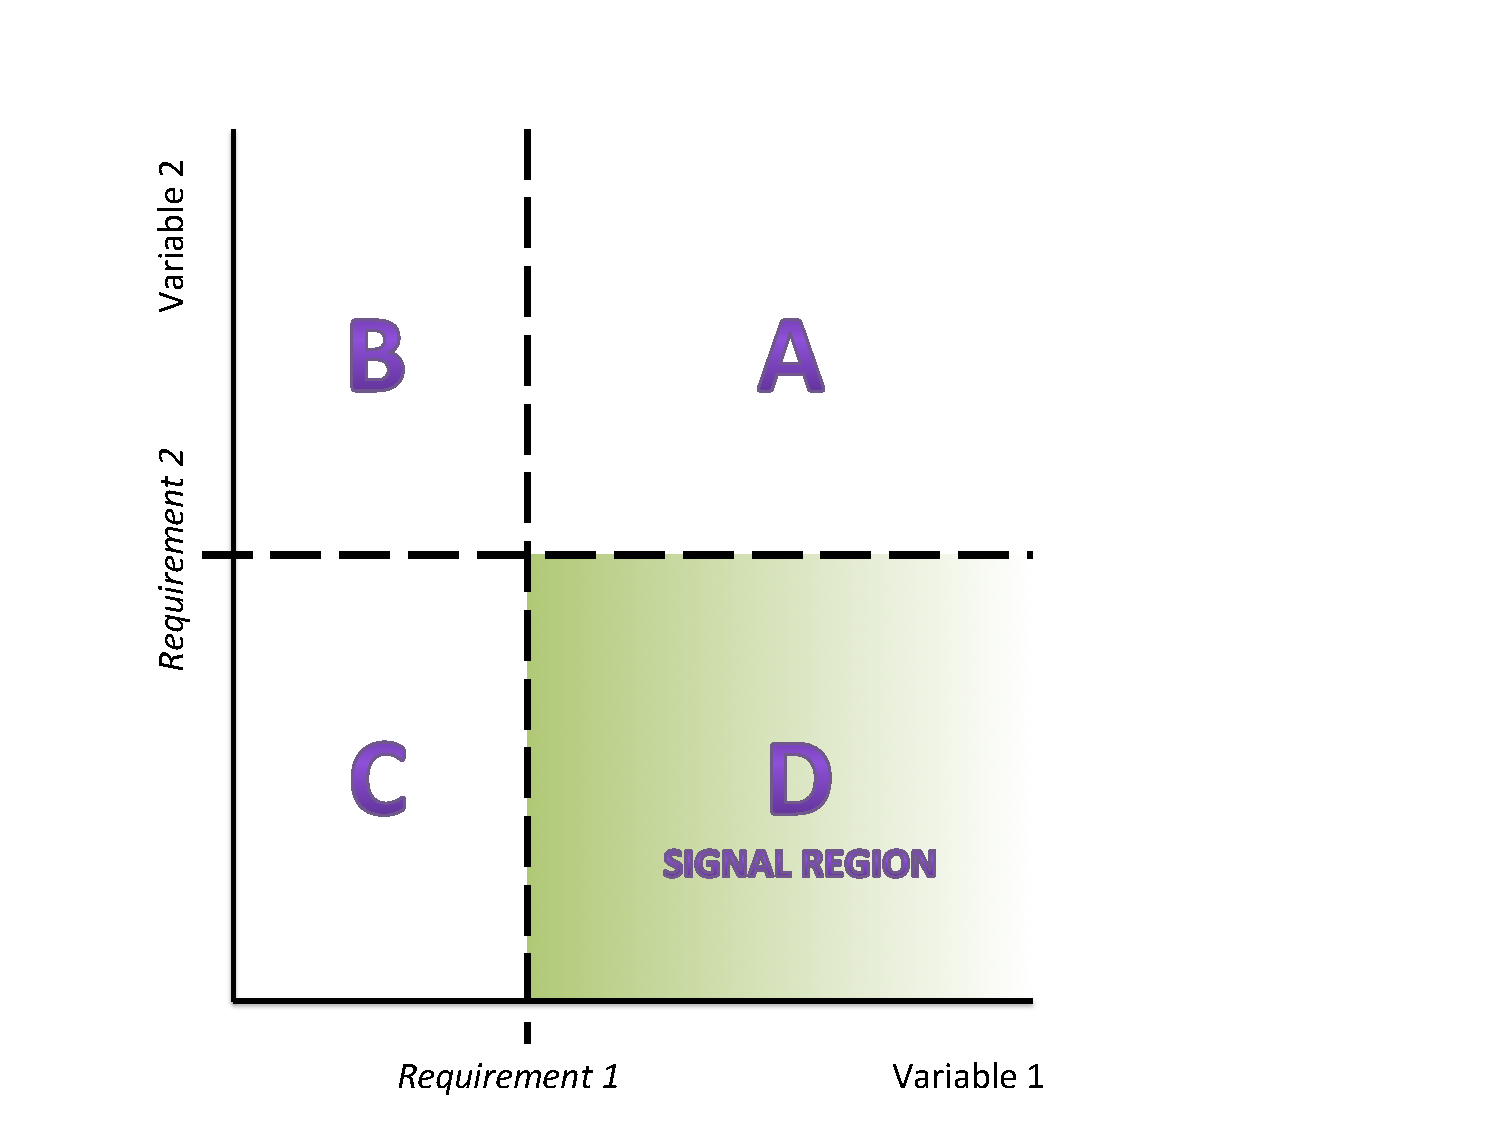
\includegraphics[width=0.6\textwidth]{images/Analysis/ABCD-req.pdf}
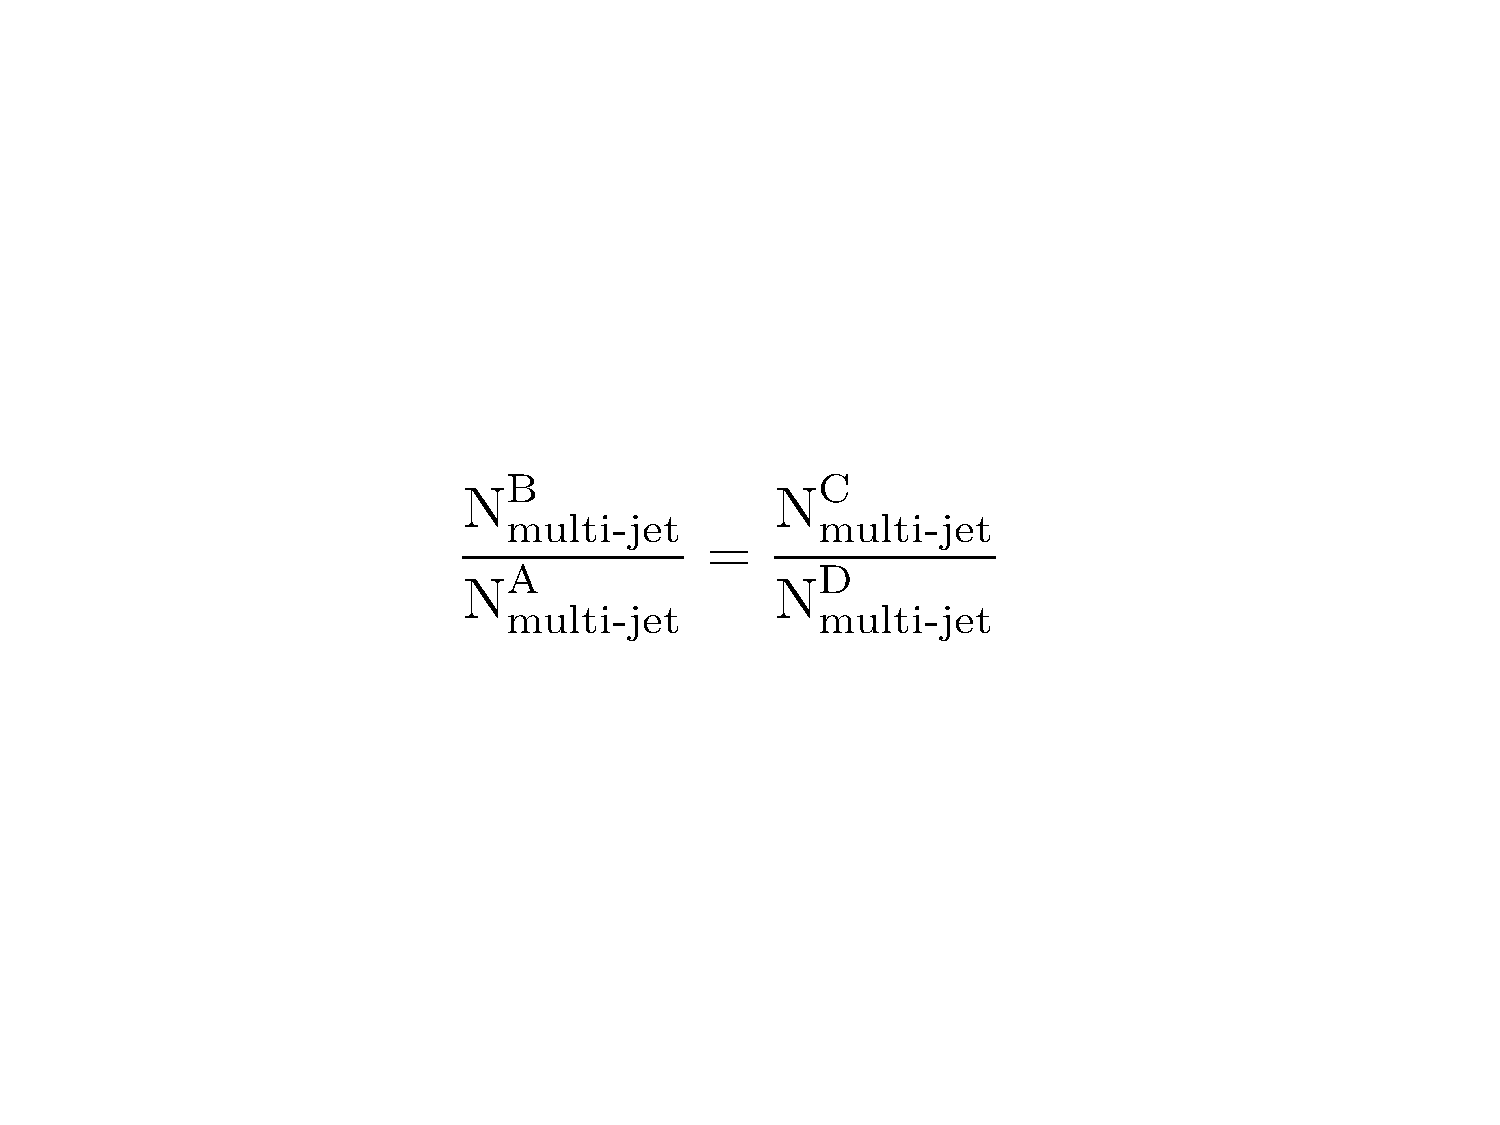
\includegraphics[width=0.6\textwidth]{images/Analysis/ABCD2.pdf}
}
\hspace{0.2cm}
\end{center}
\caption{Illustration of ABCD method}
\label{fig:ABCDdiagram}
\end{figure}

% \begin{equation}
% \frac{\textrm{N}^{\textrm{B}}_{\textrm{multi-jet}}}{\textrm{N}^{\textrm{A}}_{\textrm{multi-jet}}} = \frac{\textrm{N}^{\textrm{C}}_{\textrm{multi-jet}}}{\textrm{N}^{\textrm{D}}_{\textrm{multi-jet}}}
% \label{N-multi-jet}
% \end{equation}
For the background processes that are much more well modelled in simulation than QCD events, their yields in each region are subtracted from the data. This should in theory leave only QCD multijet events remaining and so the number of events in the signal region can be estimated from the equation in Fig.~\ref{fig:ABCDdiagram}. This method does have some dependence on the simulation and assumes that the other backgrounds are well modelled. The uncertainty on this assumption can be taken into account by varying the main \ttbar background by its main source of uncertainty. 


\section{Multi-variate analysis techniques ~\label{sec:MVAtechniques}}

Four top quark production events are very rare at the energies of $\sqrt{s} = $ 8~TeV and 13~TeV studied in this thesis. Typically, within the selection defined in Section~\ref{sec:Strategy} the main background is \ttbar production which is five orders of magnitude larger than the \tttt signal. In this type of analysis where the background and signal can be similar in many distributions and the signal is so rare, it can be advantageous to use multivariate analysis (MVA) methods to increase the signal to background separation. The main MVA method used in this thesis is \emph{Boosted Decision Trees} (BDT) where more details of this algorithm and its specific use in this analysis are given in the subsequent sections.


\subsection{Boosted Decision Trees}
\label{sec:BDT}

To start with, the simpler concept of a single Decision Tree will be considered. Decision trees are used to maximise the separation between a signal ($S$) sample and a background ($B$) sample by looking at a set of distributions in which there is some initial separation between the two; a training sample for each is provided to the algorithm. A simple decision tree is shown in Fig.~\ref{fig:DecisionTree} where each decision is defined at a \emph{node} and splits the dataset in two by placing a requirement in the most discriminating variable in order to separate as much background down one side and signal down the other side.
One can define the purity at each node as $P=\frac{S}{S+B}$. Another useful measure is the \emph{gain} at each node which gives a more symmetric measure of the node having high purity of either signal or background. The particular metric of gain used in this analysis is the commonly used \emph{Gini Index} which is defined as $Gini = P\cdot\left(1-P\right)$. A high Gini Index suggests the node contains a relatively equal amount of signal and background whereas a low Gini index shows that the node contains more of either signal or background. 
The goal is to scan across each distribution and find the requirement in the associated variable which maximises the \emph{separation gain} ($S_{G}$) as defined in equation~\ref{eqn:SepGain}. This process is iterated upon until a predefined end condition such as the maximum depth of the tree or the minimum number of events in a node.


% \begin{equation}
% P=\frac{S}{S+B}
% \label{eqn:Purity}
% \end{equation}

% \begin{equation}
% Gini = P\cdot\left(1-P\right)
% \label{eqn:Gini}
% \end{equation}

\begin{equation}
S_{G} = Gini(\textrm{parent}) - Gini(\textrm{child 1}) - Gini(\textrm{child 2})
\label{eqn:SepGain}
\end{equation}

\begin{figure}[h!]
\begin{center}
\subfloat{
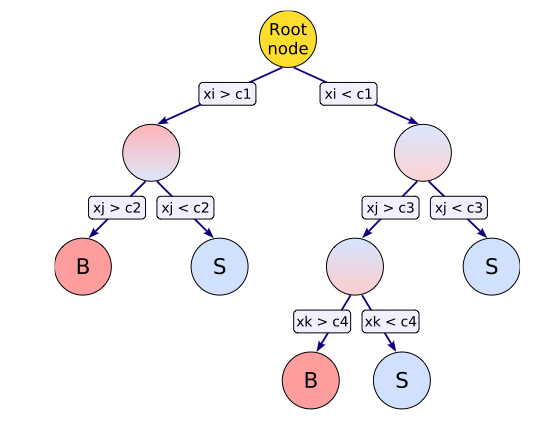
\includegraphics[width=0.67\textwidth]{images/Analysis/BDTFlow.png}}
\hspace{0.2cm}
\end{center}
\caption{Illustration of a single decision tree of depth = 3~\cite{2007physics3039H}.}
\label{fig:DecisionTree}
\end{figure} 

It has been found that using an ensemble (usually several hundred) of smaller decision trees of depth = 2 or depth = 3 is preferable to using one large decision tree as it can minimise \emph{overtraining}, ie. the propensity to train to the specific features of the training sample rather than the general trend. 

The first tree begins as a normal decision tree as described above and it terminates when it reaches the maximum depth defined. The error rate, $R_{err}$, of the tree is defined as the number of events incorrectly classified divided by the total number of events. The events which were incorrectly categorised are weighted according to equation~\ref{eqn:ErrorWeight} where $\alpha$ is the \emph{boost weight} which is dependent on $R_{err}$. The idea is that in the next iteration of a tree the incorrectly classified events are considered with higher importance. The degree of boosting can be adjusted by raising $\alpha$ to the power of $\beta$, the learning rate.

\begin{equation}
\alpha = \left( \frac{R_{err}}{R_{err}}  \right)
\label{eqn:ErrorWeight}
\end{equation}

This process is repeated until the predefined maximum number of trees has been reached. 

A discriminator value, $y_{BDT}$, is defined by summing the response from each tree, \emph{t}, and weighting each response by $\ln \left(\alpha_{t}\right)$ such that the trees with low error rates are considered more than trees with high error rates. The response from each individual tree is defined as $h\left(\textbf{x}\right)$ where $h\left(\textbf{x}\right) = +1 \textrm{ for signal and} -1 \textrm{ for background}$ and $\textbf{x}$ is the set of input variables. 

\begin{equation}
y_{BDT} = \frac{1}{Ntrees} \cdot \sum_{t}^{Ntrees} \ln \left(\alpha_{t}\right) \cdot h_{t}\left(\textbf{x}\right)
\end{equation}

Values of $y_{BDT}$ which are closer to +1 (-1) are considered to be more signal-like (background-like).

\subsection{Reconstruction of hadronic top quarks \label{sec:topreco}}

In \tttt single lepton channel there are three hadronically decaying top quarks while there is only one hadronically decaying top quark in the semi-leptonic \ttbar final state. Equivalently in the dilepton channel there are two (zero) hadronically decaying top quarks in \tttt (\ttbar). Therefore reconstructing top quarks from their hadronic decay products should be a powerful way to separate the signal and background processes. The jets which are in addition to the hard process in \ttbar are likely to come from initial or final state radiation (ISR or FSR) or from pileup, hence it should be unlikely to reconstruct a hadronic top quark from these additional jets. Due to the large number of jets within the selection, it is difficult challenge to find the right combination of jets which originated from a top quark. This motivates using multivariate analysis in order to rank each combination of three jets (tri-jet) according to which is most likely to be the combination that originated from a real hadronically decaying top quark.
A training sample from \ttbar events is provided to the BDT where the Monte Carlo truth information is used to classify whether a tri-jet combination was a \emph{good} combination which originated from a top quark or a \emph{bad} combination which is formed from random jets. The following variables were selected for use within the BDT:\\
\textbf{Tri-jet invariant mass} - Good tri-jet combinations should have an invariant mass distribution which peaks around the top mass.
Bad tri-jet combinations will have a much broader distribution. \\
\textbf{Di-jet invariant mass} - The di-jet combination is formed from the two jets with the smallest \DR separation. The invariant mass distribution should peak around the W mass for good tri-jet combinations.\\
\textbf{\ptrat} - This is the ratio of the vectorial \pt to the scalar sum of the \pt of the jets in the tri-jet combination. This is likely to be smaller in a random combination of jets where the vectorial \pt of each jet will cancel out more than in a good tri-jet combination.\\
\textbf{\DPTW} - This is the \Dphi between the tri-jet and di-jet system which should be smaller in good tri-jet combinations.\\
\textbf{\DPTb} - This is the \Dphi between the tri-jet and remaining jet not included in the di-jet system which should be smaller for good tri-jet combinations.\\
\textbf{\CSVj} - For the jet not used in the di-jet system, the CSV b-tagging discriminator value is used. If the di-jet system correctly identifies the quark jets coming from a W boson decay then the remaining jet in a good tri-jet combination should be a b-jet and hence will have a higher CSV b-tagging discriminator than a typical randomly selected jet.\\
The BDT algorithm is trained on the six variables above. It produces a discriminator value for each tri-jet combination. Higher BDT discriminator values are associated with the jets being more likely to have come from a top quark. Each tri-jet combination is ranked according to the BDT discriminator value. In the dilepton channel the value for the highest ranked tri-jet, known as BDT$_{tri-jet1}$, can be used as a discriminating variable between \tttt and \ttbar. In the single lepton channel the three jets which make up the highest ranked tri-jet combination are removed from the collection of jets and the process is repeated. The discriminator value of the next highest ranked tri-jet, BDT$_{tri-jet2}$, in this reduced jet collection can be used to distinguish between \tttt and \ttbar.

\subsubsection{Reduced Variables}
As mentioned above, BDT$_{tri-jet2}$ is calculated from a reduced jet collection where the three jets from the highest-ranked tri-jet are removed from the jet collection. In \ttbar events, the removal of the jets most likely to form a true top quark leave softer jets remaining in the reduced jet collection, usually from ISR, FSR or PU rather than the hard process of \ttbar production. In \tttt events the removal of the leading hadronic top quark candidate potentially leaves behind two additional hadronic top quarks, where some of the jets may not be reconstructed but there should still be harder jets from the hard process than what remains in \ttbar events. Therefore some discriminating variables can be formed from the reduced jet collection, as follows:

\textbf{HT$_{X}$} - This is the \HT of the reduced event which should be higher for signal \tttt events.\\
\textbf{\sumjetmassX} - Invariant mass of all jets contained in the reduced event which should be higher for signal \tttt events..

\subsection{Event-level BDT}

A second BDT is employed to increase the separation between the \ttbar background and \tttt signal beyond what can be achieved with a simpler variable. Several discriminating variables have already been formed from the hadronic top reconstruction; BDT$_{tri-jet1}$, BDT$_{tri-jet2}$, HT$_{X}$, \sumjetmassX. More discriminating variables can be formed from the event information, as follows:

\textbf{b-jet content}\\
As the branching ratio of top quarks to a b quark and a W boson is $\approx 100\%$, the main background process, \ttbar + \llbar,  typically produces two b-quarks while \tttt, typically produces four. Hence, the presence of more than two b-tagged jets is a potentially important source of discriminating power.
At 8~TeV this was exploited by looking at the number of CSVM b-tags in an event, \nMtags. At 13~TeV the CSV values for the \emph{third-highest CSV} and \emph{fourth-highest CSV} are used to discriminate between signal and background and it is expected that these values will be lower for \ttbar + \llbar events where the third-highest CSV and fourth-highest CSV are not likely to be b-jets. However for \ttbar + \bbbar events these variables do not provide much discrimination power.
Another variable used is the scalar sum of the \HT of all CSVM b-jets in the event which should be higher for \tttt events, \htb.

\textbf{Event-Activity}\\
One of the most obvious variables to choose to distinguish between \ttbar and \tttt is the number of jets (\njets) as on average \tttt events have a higher number of jets than \ttbar. In semi-leptonic \ttbar events there are up to four hard jets from the hard process compared to up to ten from \tttt, so the fifth and sixth jet \pt can be used to distinguish between the event types. The same idea is used to form the variable \htrat which is the ratio of the scalar sum of the \HT from the four highest \pt jets to the scalar sum of the \HT of the other jets in the events. This variable should be smaller for \tttt events where there are more than four jets coming form the hard process.
The \emph{centrality} of the event is defined as the ratio of the \HT in the event to the H in the event, where H is the scalar sum of the total momentum (P) in the event.

The lepton \pt is used as a training variable as it is slightly larger in \tttt events than in \ttbar events.

The \emph{Weighted jet multiplicity} (\njetsw) takes into account a combination of the \pt spectra of the jets and the differences in the jet multiplicity. It is sensitive to the differences between the \pt spectra of the jets from a top quark decay and those originating from ISR/FSR. The \njetsw definition is given in equation~\ref{eqn:WjetMul} where $p_T^{th}$ is the \pt threshold above which a jet is counted, $N_j\left(p_T > p_T^{th}\right)$ is the number of jets above the \pt threshold, $p_T^{low(up),i}$ takes values from the set [30 \GeV; $p_{T,1}$; $p_{T,2}\cdots$; $p_{T,N_j}$] ([$p_{T,1}$; $p_{T,2}\cdots$; $p_{T,N_j}$; 125 \GeV]), given that $p_{T,i}$ is the \pt of each jet in ascending order. The kinematic threshold is determined by the median jet \pt. The prefactor arises from the integral in the denominator combined with constant factors in the numerator.

\begin{equation}
% old version:	N_j^W = \frac{\int_{30}^{125}{N_j\left(p_T\mathrm{[GeV]} > p_T^{th}\right)\cdot p_T^{th}\,dp_T^{th}}} {\int_{30}^{125}{ p_T^{th}\,dp_T^{th}}} = \frac{1}{14725}\sum_{i=1}^{N_{jets}}{N_j\left(p_T\mathrm{[GeV]}>p_T^{low,i}\right)\cdot\left.\left(p_T^{th}\right)^2\right|^{p_T^{up,i}}_{p_T^{low,i}}},
N_j^W = \frac{\int_{30}^{125}{N_j\left(p_T > p_T^{th}\right)\cdot p_T^{th}\,dp_T^{th}}} {\int_{30}^{125}{ p_T^{th}\\
,dp_T^{th}}} = \frac{1}{14725}\sum_{i=1}^{N_{jets}}{N_j\left(p_T>p_T^{low,i}\right)\cdot\left.\left(p_T^{th}\right)^2\right|^{p_T^{up,i}}_{p_T^{low,i}}},  
\label{eqn:WjetMul}
\end{equation} 


\textbf{Training}\\
Each analysis from the single-lepton channel at 8~TeV, the single-lepton channel at 13~TeV and the dilepton channel at 13~TeV, uses different subsets of the variables described above. The variables which are only used in the dilepton channel have not been described here and can be found in \fxnote*{make appendix}{Appendix} The optimised set of variables for each training are provided to the TMVA package where the AdaBoost boosting algorithm is employed. The \tttt signal is trained against the main \ttbar background only as the other backgrounds are comparatively small. The \emph{event-level} BDT will return a discriminator value which will be closer to +1 (-1) for signal-like (background-like) events.

\section{Systematic uncertainties}
\label{sec:uncertainties}

Both the modelling of the simulation and the efficiency of the detector are not perfect and hence they bring some uncertainty to the measurement which needs to be taken into account when fitting the simulation to the data as described in section~\ref{sec:limitFit}.
There are two categories of systematic uncertainties; (i) Uncertainties which affect the normalisation of the distributions and (ii) uncertainties which affect the shape of the distributions. The quantity causing the uncertainty in each case can be varied up and down to produce alternative histogram templates.

\subsection{Normalisation uncertainties}
%The normalisation uncertainties will only affect the uncertainty on the expected limit rather than the limit itself when it is used in the template fit and limit setting procedure described in Section~\ref{sec:limit}.
Normalisation uncertainties include the following:
\begin{itemize}
\item \textbf{Luminosity}\\
There is some uncertainty on the luminosity as measured by the CMS Luminosity group which affects the normalisation of all simulation samples as they are scaled to the measured luminosity

% The CMS Luminosity Group give a recommendation of 2.6$\%$ uncertainty on the luminosity~\cite{CMS-PAS-LUM-12-001}.
\item \textbf{Monte Carlo simulation cross sections}\\
There is uncertainty on the cross sections given for each of the background processes due to uncertainty in the renormalisation and factorisation scale and the PDF uncertainty. As \ttbar is the main background to \tttt, the uncertainty on its MC cross-section is expected to be dominant over the other background processes. 

\item \textbf{Lepton ID, Iso and trigger SF}\\
An uncertainty arises from the choice of lepton triggers and identification criteria in the baseline selection which is applied to all simulation data sets.

%The uncertainty on \ttbar is ${}^{+2.5\%}_{-3.4\%} \left( \textrm{renormalisation and factorisation scale} \right)$ and ${}^{+2.5\%}_{-2.6\%} \left( \textrm{PDF} \right)$~\cite{PhysRevLett.110.252004}.
%\fxnote*{??}{The MC cross section uncertainties are modelled by assigning a $4\%$ uncertainty to each background process and a $10\%$ uncertainty to the signal process}
\end{itemize}

\subsection{Shape uncertainties}
 Shape uncertainties arise from the following quantities.
\begin{itemize}
\item \textbf{Factorisation and renormalisation scales}
This factorisation and renormalisation scale $\left(\mu_{f},\mu_{s}\right)$ can be shifted up and down at matrix element (ME) level and at parton shower (PS) level within the simulation. A shift in the $Q^{2}$ scale at PS level is equivalent to changing the value of $\alpha_{S}$ so the uncertainty from the jet multiplicity modelling in section~\ref{subsec:alphaS} can be included by inflating the PS scale systematic.

\item \textbf{Matching threshold}\\
The uncertainty due to the choice of matching threshold between the matrix element calculation and the parton shower is evaluated by producing alternative simulation samples where the matching threshold is varied between 20~GeV and 40~GeV.

\item \textbf{Generator choice}\\
The uncertainty on the choice of generator for the main \ttbar background is evaluated by considering an alternative \ttbar MC generator. The difference between the number of events in each bin of the output BDT distributions is converted into a symmetric uncertainty around the template created by the chosen MC generator.

\item \textbf{Jet Energy Scale}\\
The uncertainty on the \fxnote*{mentioned elsewhere?}{Jet Energy Corrections} applied to the simulation is evaluated by varying the Jet Energy Scale (JES) by $\pm 1\sigma$.

\item \textbf{JER}\\
The energies of the jets in simulation are smeared to match the observed discrepancy between the jet energy resolution, JER, in data and simulation. The amount the jet energies are smeared by is varied by $\pm 1\sigma$.

\item \textbf{b tagging}\\
There is a significant uncertainty on the measurement of b-tagging scale factors which is particularly important as variables derived from b-tagging jets are used in the event-level BDT. The method of accounting for this uncertainty varies depending on the b-tag modelling used from section~\ref{sec:btagModelling}.

\item \textbf{Pile up}\\
The minimum bias cross section used in the simulation which is used to derive the pile up scale factors is varied by $\pm 5\%$ to account for uncertainty on the minimum bias cross section. 

\item \textbf{\heavyflavourone~/~\heavyflavourtwo modelling}\\
The uncertainty on the measurement of the ratio of \heavyflavourone~/~\heavyflavourtwo is translated into an uncertainty on the scale factors applied to heavy flavour jets. An anti-correlated uncertainty is applied to light flavour jets.

\end{itemize}

The subsets of this list of uncertainties used for the \runone and \runtwo analyses and which data sets they are applied to are described in sections~\ref{c:Run1} and~\ref{c:Run2}. 

% The analysis procedure is repeated with \ttbar samples which have the respective quantity varied by $\pm 1 \sigma$ in order the produce new BDT templates with a deviated shape However, in the case of the matching threshold, the alternative shapes are produced by varying the matching threshold up to 40 GeV and down to 20 GeV.

\section{Limit setting \label{sec:limitFit}}
So far we have the nominal histogram templates in the BDT output discriminator disctribution for each background and signal, the normalisation systematic uncertainties for each source, and the alternative histograms for the up and down shape systematic uncertainties. All of these quantities are entered in the Higgs Combine Tool based on the Roostats package where a Maximum Likelihood Fit (MLF) is performed. In reality the MLF actually minimises the negative log likelihood ($-\ln\mathcal{L}$) as it is computationally simpler to work with.

The expected number of events in bin $i$, $\mu_{i}$, is given in equation~\ref{eqn:expectedmui} where L is the luminosity, $\sigma_{j}$ is the cross section for the source of events from process $j$, and $\epsilon_{ij}$ is the efficiency for source $j$ to be in bin $i$ derived from simulation

\begin{equation}
\mu_{i} = \sum_{j=1}^{n_{source}}L\sigma_{j}\epsilon_{ij}
\label{eqn:expectedmui}
\end{equation}

If we assume that the number of events in bin $i$, $n_{i}$, will be gaussian-distributed ($\mathcal{G}$) then the likelihood for the entire histogram is given in equation~\ref{eqn:gausslike}.
\begin{equation}
\mathcal{L} = \prod_{i=1}^{N} \mathcal{G}\left(n_{i}|\mu_{i},\sigma_{i}\right)
\label{eqn:gausslike}
\end{equation}

Each systematic uncertainty is modelled as a nuisance parameter in the fit. Normalisation uncertainties are modelled as lognormal nuisance parameters which is generally preferable to using a gaussian nuisance parameter as it is better at modelling multiplicative uncertainties and does not allow the parameter to become negative. The shape uncertainties are modelled using vertical morphing between the three templates; the nominal which has efficiency $\epsilon_{ij}^{0}$, systematic shifted up with efficiency $\epsilon_{ij}^{+}$ and systematic shifted down with efficiency $\epsilon_{ij}^{-}$. Quadratic interpolation is used between the two systematic templates and linear extrapolation beyond that range. The quadratic interpolation is shown in equation~\ref{eqn:VerticalMorphing} where morphing parameter $f$ has an Gaussian uncertainty with $\sigma_{f}=1$.

\begin{equation}
\epsilon_{ij} = \frac{f\left(f-1\right)}{2}\epsilon_{ij}^{-} - \left(f-1\right)\left(f+1\right) \epsilon_{ij}^{0}  \frac{f\left(f+1\right)}{2}\epsilon_{ij}^{+}
\label{eqn:VerticalMorphing}
\end{equation}

From the MLF, the number of background events from each source and the number of signal events can be extracted from the \emph{post-fit} distributions

\subsection{\CLS method}




\subsection{Categorisation}
\label{sec:Cats}

Categorising events according to the numbers of jets and b-tags and hence producing more BDT templates to go into the fit allows the main \ttbar background to be constrained in the signal-depleted regions whereas the signal sensitivity will be increased in signal rich and background-depleted regions.




\chapter{Search for standard model~\tttt production in \runone at $\sqrt{s} =$~8~TeV }
\label{c:Run1}

\section{Introduction}
In this chapter, an analysis of the full 2012 CMS data set of proton-proton collisions at $\sqrt{s} =$~8~TeV with 19.7~\fbinv of data is presented where the SM production of four top quarks (\tttt) is sought. SM \tttt production has a cross section of $\sigmattttSM \approx 1.3$ fb at NLO with NNLO corrections~\cite{Barger201070,Bevilacqua2012}. 

% this equates to approximately 26 events in the 2012 dataset in all decay channels. However, in this analysis, only final states where one of the top quarks decays leptonically into an electron or muon are considered. These are referred to as the single lepton channels and they are the most prevalent decay mode as can be seen in ~\fxnote*{add fig}{figX}. One of the main challenges of this analysis is to distinguish this extremely rare signal process with the overwhelmingly large background process of top-pair production (\ttbar) which is five orders of magnitude greater than the \tttt signal process, the latest measurement putting it at $241.5 \pm 8.5$ \pbinv ~\cite{CMS-PAS-TOP-14-016}. 


%This analysis proceeds as follows; Section~\ref{sec:sigback} discuss the \tttt signal processes and the relevant background and Section~\ref{sec:datasimulation} describes the datasets and simulations of the signal and backrgound used. Section~\ref{sec:baseline} details the initial requirements imposed on the signal region while Section~\ref{sec:Calibrations} describes the calibrations made to the correct the simulation. The multi-jet background estimation is described in Section~\ref{sec:QCDbackground} and the multi-variate techniques used to increase the discrimination power between signal and background are contained in~\ref{sec:discriminating}. Discussion of the systematic uncertainties and extraction of the limit on the \tttt cross section are in Sections~\ref{sec:uncertainties} and~\ref{sec:limit}. Validation of the analysis can be found in Section~\ref{sec:signalinjection}. Finally, a summary and discussion of the ATLAS \tttt cross section limit can be found in Sections~\ref{sec:summary} and~\ref{sec:ATLASresult}.
Sections~\ref{sec:QCDbackground},~\ref{sec:njetcatlimit} and~\ref{studies8} are the authors personal contribution to the analysis.

%An initial baseline selection of requirements on the number of leptons, jets, b-tagged jets, transverse hadronic energy (\HT) and transverse missing energy (\MET) reduces the \ttbar background to three orders of magnitude greater than the \tttt signal. As \ttbar remains a very large background, multi-variate techniques are employed to reconstruct top quarks and then ultimately to find a discriminator value to distinguish between signal and background.
%In the absence of an excess of events over background, the \CLS method is used to obtain an observed limit on the cross section of \tttt production of 32 fb at 95\% confidence level compared to 32$\pm17$ fb expected.



\section{Data and Simulation}
\label{sec:datasimulation}
This analysis uses data from proton-proton collision at the CMS experiment in 2012 at $\sqrt{s}=8$~TeV.
For the muon (electron) channel, the data were collected using a trigger based on the presence of at least one muon (electron) candidate with $\pt > $ 24 (27) GeV and correspond to an integrated luminosity of 19.7 \fbinv .
% The full 2012 SingleElectron dataset is used for the electron channel, which requires an electron candidate with $\pt > $ 27 GeV and corresponds to an integrated luminosity of 19.7 \fbinv.
The signal SM \tttt Monte Carlo (MC) samples and the background MC samples are given in Table~\ref{tab:datasets_sim_8tev}, along with the MC generators used to produce these samples, the order at which they were produced and the number of events produced. MC samples were produced for the scale and matching systematics, these can be found in Table~\ref{tab:datasets_sys_8tev}. In this analysis the scale uncertainty includes the ME scale and PS scale.


\begin{table}[ht!]
% \tiny
\centering
\begin{tabular}{| l | l | l | p{2cm} |}
 \hline 
 Dataset & Events & Generator & Order \\
\hline
\tttt & 100K & \MADGRAPH $+$ \TAUOLA& O \\
\hline
\ttbar Semi leptonic &25M & \MADGRAPH $+$ \TAUOLA & O \\
\hline
\ttbar Hadronic &31M & \MADGRAPH  $+$ \TAUOLA& O \\
\hline
\ttbar Dileptonic & 12M & \MADGRAPH  $+$ \TAUOLA& O \\
\hline
W + 4 Jets $\rightarrow$ l$\nu$ & 13M & \MADGRAPH & O \\
\hline
${\overline{\textrm{t}}}$ tW-channel & 500K & \POWHEG $+$ \TAUOLA & O\\
\hline
t tW-channel & 500K & \POWHEG $+$ \TAUOLA & O \\
\hline
t t-channel & 3.8M & \POWHEG $+$ \TAUOLA & O \\
\hline
${\overline{\textrm{t}}}$ s-channel & 260K & \POWHEG $+$ \TAUOLA & O \\
\hline
t s-channel & 139K & \POWHEG $+$ \TAUOLA & O \\
\hline
${\overline{\textrm{t}}}$ t-channel & 2M  & \POWHEG $+$ \TAUOLA & O \\
\hline
% DY4JetsToLL & 6.2M & \MADGRAPH & O  \\
% \hline
DYJets $\rightarrow~ll$  & 6.7M & \MADGRAPH & O \\
\hline
TTZ  & 200K & \MADGRAPH & O \\
\hline
TTW\ & 200K & \MADGRAPH & O \\
\hline
TTH$\rightarrow$ HToBB & 1M & \PYTHIA 6 $+$ \TAUOLA & O \\
\hline
ZZ & 10M & \PYTHIA 6 $+$ \TAUOLA & O \\
\hline
WZ &10M & \PYTHIA 6 $+$ \TAUOLA & O \\
\hline
WW &10M & \PYTHIA 6 $+$ \TAUOLA & O \\
\hline
\end{tabular}
 \caption{Dataset name, total number of events, MC generator and order of the simulated samples.}
  \label{tab:datasets_sim_8tev}
  \end{table}


\begin{table}[ht!]
% \tiny
\centering
\begin{tabular}{| l | l | l | p{2cm} |}
 \hline 
 Dataset & Events & Generator & Order \\
\hline
\ttbar scale down & 5M  & \MADGRAPH $+$ \TAUOLA & O \\
\hline
\ttbar scale up & 5M  & \MADGRAPH $+$ \TAUOLA & O \\
\hline
\ttbar matching down & 5M & \MADGRAPH $+$ \TAUOLA & O  \\
\hline
\ttbar matching up & 5M & \MADGRAPH $+$ \TAUOLA & O \\
\hline
\end{tabular}
 \caption{Dataset name, total number of events, MC generator and order of the simulated systematic samples.}
  \label{tab:datasets_sys_8tev}
\end{table}
\section{Baseline Event Selection}
\label{sec:baseline}
To select \tttt events and suppress background events, a set of criteria is applied to the reconstructed objects in events which are triggered by the single muon or single electron triggers.
For the muon channel these are:
\begin{itemize}
\setlength\itemsep{0em}
\item Exactly one tight muon
\item Exactly zero additional loose muons
\item Exactly zero loose electrons
\item At least 6 jets with $\pt >$ 30 \GeV
\item At least 2 CSVM tagged b-jets
\item $\HT > $ 400 \GeV 
\item $\MET > $ 30 \GeV 
\end{itemize}
For the electron channel these are:
\begin{itemize}
\itemsep0em 
\item Exactly one tight electron
\item Exactly zero additional loose electrons
\item Exactly zero loose muons
\item At least 6 jets with $\pt >$ 30 \GeV
\item At least 2 CSVM tagged b-jets
\item $\HT > $ 400 \GeV 
\item $\MET > $ 30 \GeV 
\end{itemize}

\section{Corrections to the simulation}
\label{sec:Calibrations8}
All corrections are described in section~\ref{sec:Calibrations}.
The events for all background and signal samples which pass the baseline event selection are given a weight which is the product of the weights for the pile up corrections, a weight to correct the b-tag modelling from the method in ~\ref{subsec:method1btag} and a weight for lepton modelling corrections. The heavy flavour jet modelling from section~\ref{ttbbmod} is applied to the \ttbar background.



% \subsection{b tag modelling}

% There are significant differences between b tag efficiencies measured by CMS in data and the efficiencies as measured in simulation. To account for this, a weight must be applied applied to the selected MC events in order to predict the correct event yield in data. The full method can be found in this reference~\cite{CMS-PAS-BTV-13-001}.

% \subsection{Heavy flavour jet modelling}

% There is a discrepancy between data and simulation in the tails of the \fxnote*{show unweighted}{distribution} of the number of b-tagged jets (\nbtags) which suggests that the amount of heavy flavour jets in \ttbar events is incorrectly simulated. The ratio of \heavyflavour was measured by CMS to be $2.2 \pm 0.3 \left( \textrm{stat.} \right) \pm 0.5 \left(\textrm{sys.} \right)\% $ ~\cite{CMS:2014yxa} at $\sqrt{s} =$ 8TeV. To incorporate this ratio into the analysis, the MC truth information of the \ttbar$+$jets MC sample is used to split the sample into \ttbb, \ttcc and \ttll, where l denotes light quarks and gluons (\cPqu, \cPqd, \cPqs, \cPg) . Weights are applied to each sub-sample to match the measured ratio whilst preserving the total number of \ttbar events. After this procedure is applied, the agreement between data and simulation in the \nbtags distribution is improved as can be seen in Fig~\ref{fig:datasimnbtags}.

% \subsection{Lepton modelling}
% Due to a difference between data and simulation in the efficiency of lepton identification and isolation, a weight is applied to events which is dependent on the selected leptons $\eta$, $\pt$ and lepton flavour.
\section{Effect of selection requirements \label{cutflow}}

The event counts, after weighting, are given for the muon (electron) channel in Table~\ref{tab:museltable8} (Table~\ref{tab:eseltable8}). It is quite evident that the main background is \ttbar production, with smaller contributions coming from W$+$jets, Z$+$jets and single top (ST) as well as almost negligible contributions from the diboson and TT+X background (X $=$ H, Z, W).




\begin{table}
\tiny
\caption{Number of events after successive selection requirements in the $\mu$ + jets channel ($\mathcal{L}=19.6~\fb$)}
\label{tab:museltable8}
\centering
\begin{tabular}{|c|c|c|c|c|c|c|c|c|c|c|c|c|}
\hline
&$Data$ &$\tttt$  &$ttH$  &$Wjets$ &$Zjets$ &$ST$ &$WW$ &$WZ$ &$ZZ$ &$TTZ$  &$TTW$  &$\ttbar$ \\
\hline
Trigger and PV&  120508  &4.5  &171.8  &16094  &3916.3 &3256.2 &272.0  &161.1  &71.5 &219.3  &277.5  &84476  \\

1 iso. $\mu$& 95723 &3.5  &141.6  &13655  &2635.1 &2750.2 &232.7  &125.0  &47.6 &168.5  &229.3  &70030  \\

Loose $\mu$ veto& 93385 &3.2  &138.9  &13654  &1835.3 &2739.2 &232.3  &114.7  &34.0 &153.5  &222.9  &69503  \\

Loose e veto& 91546 &2.5  &132.6  &13593  &1812.0 &2691.6 &228.9  &113.0  &33.3 &143.6  &206.0  &68040  \\

\njets $\geq$ 6 &  24791 &2.3  &59.1 &2428.4 &350.7  &591.9  &41.5 &20.0 &5.1  &71.8 &94.1 &21197  \\

\nMtags $\geq$ 2 &  9260  &1.7  &46.0 &68.8 &15.2 &215.5  &3.1  &1.4  &0.6  &35.0 &39.5 &9138.8 \\

HT $\geq$  400 GeV& 6342  &1.6  &37.7 &49.3 &10.4 &156.9  &2.6  &1.0  &0.4  &29.6 &32.8 &6542.2 \\

\MET $\geq$  30 GeV&      5215  &1.5    &31.7   &41.5   &7.1    &132.2  &2.2    &0.9    &0.1    &24.4   &28.3   &5415.1 \\
\hline
\end{tabular}
\end{table}

\begin{table}
\tiny
\caption{Number of events after successive selection requirements in the $e$ + jets channel ($\mathcal{L}=19.6~\fb$)}
\label{tab:eseltable8}
\centering
\begin{tabular}{|c|c|c|c|c|c|c|c|c|c|c|c|c|}
\hline
&$Data$ &$\tttt$  &$ttH$  &$Wjets$ &$Zjets$ &$ST$  &$WW$ &$WZ$ &$ZZ$ &$TTZ$  &$TTW$  &$\ttbar$  \\
\hline
Trigger and PV& $1128500$ &$8.6$  &$307.8$  &$28831$  &$25118.7$  &$6494.4$ &$683.8$  &$464.1$  &$228.3$  &$440.4$  &$545.5$  &$157087$ \\

1 iso. e& $103856$  &$3.2$  &$117.6$  &$9631.6$ &$7183.4$ &$2212.4$ &$217.6$  &$136.8$  &$60.9$ &$156.4$  &$207.4$  &$78912$  \\

Loose e veto& $100861$  &$3.0$  &$115.9$  &$9611.2$ &$5354.2$ &$2199.2$ &$216.4$  &$121.7$  &$43.7$ &$144.7$  &$201.9$  &$63812$  \\

Loose mu veto&  $99402$ &$2.3$  &$110.9$  &$9605.0$ &$5340.7$ &$2172.0$ &$215.2$  &$120.8$  &$43.3$ &$134.4$  &$186.3$  &$62584$  \\

\njets$\geq$ 6 &  $26508$ &$2.1$  &$55.2$ &$1660.3$ &$1108.3$ &$490.7$  &$32.0$ &$20.6$ &$7.2$  &$67.6$ &$84.7$ &$19776.8$  \\

\nMtags$\geq$ 2 &  $8945$  &$1.5$  &$43.2$ &$45.4$ &$19.8$ &$179.3$  &$1.3$  &$2.0$  &$0.8$  &$31.5$ &$35.6$ &$8362.1$ \\

HT $\geq$ 400 GeV&  $6278$  &$1.5$  &$35.6$ &$33.2$ &$13.9$ &$134.2$  &$1.0$  &$1.3$  &$0.5$  &$26.1$ &$29.1$ &$6061.1$ \\

\MET $\geq$ 30 GeV & $5066$  &$1.3$  &$30.0$ &$25.4$ &$7.0$  &$114.2$  &$0.8$  &$1.1$  &$0.2$  &$21.5$ &$24.5$ &$4973.9$ \\
\hline
\end{tabular}
\end{table}


% \begin{table}
% \tiny
% \caption{Number of events after successive selection requirements in the $e$ + jets channel ($\mathcal{L}=19.6~\fb$)}
% \label{tab:eseltable8}
% \centering
% \begin{tabular}{|c|c|c|c|c|c|c|c|c|c|c|c|c|c|}
% \hline
% &$Data$ &$\tttt$  &$ttH$  &$Wjets$ &$Zjets$ &$ST$  &$WW$ &$WZ$ &$ZZ$ &$TTZ$  &$TTW$  &$\ttbar_{other}$ &$\ttbar_{semi-lep}$  \\
% \hline
% Trigger and PV& $1128500$ &$8.6$  &$307.8$  &$28831$  &$25118.7$  &$6494.4$ &$683.8$  &$464.1$  &$228.3$  &$440.4$  &$545.5$  &$14569$  &$157087$ \\

% 1 iso. e& $103856$  &$3.2$  &$117.6$  &$9631.6$ &$7183.4$ &$2212.4$ &$217.6$  &$136.8$  &$60.9$ &$156.4$  &$207.4$  &$5050$ &$59293$  \\

% Loose e veto& $100861$  &$3.0$  &$115.9$  &$9611.2$ &$5354.2$ &$2199.2$ &$216.4$  &$121.7$  &$43.7$ &$144.7$  &$201.9$  &$4611$ &$59201$  \\

% Loose mu veto&  $99402$ &$2.3$  &$110.9$  &$9605.0$ &$5340.7$ &$2172.0$ &$215.2$  &$120.8$  &$43.3$ &$134.4$  &$186.3$  &$3456$ &$59128$  \\

% $>$= 6 Jets&  $26508$ &$2.1$  &$55.2$ &$1660.3$ &$1108.3$ &$490.7$  &$32.0$ &$20.6$ &$7.2$  &$67.6$ &$84.7$ &$977.8$  &$18799$  \\

% $>$= 2 b-tags&  $8945$  &$1.5$  &$43.2$ &$45.4$ &$19.8$ &$179.3$  &$1.3$  &$2.0$  &$0.8$  &$31.5$ &$35.6$ &$421.1$  &$7941$ \\

% HT $>$= 400 GeV&  $6278$  &$1.5$  &$35.6$ &$33.2$ &$13.9$ &$134.2$  &$1.0$  &$1.3$  &$0.5$  &$26.1$ &$29.1$ &$321.4$  &$5739.7$ \\

% \MET $>$ 30 GeV & $5066$  &$1.3$  &$30.0$ &$25.4$ &$7.0$  &$114.2$  &$0.8$  &$1.1$  &$0.2$  &$21.5$ &$24.5$ &$297.0$  &$4676.9$ \\
% \hline
% \end{tabular}
% \end{table}




\section{Control distributions between data and simulation}

% After the baseline event selection, events are weighted using the prescription for pile-up as described in Section~\ref{sec:pile-up}. The weights are applied for b-tagging, the heavy flavour jet modelling and the lepton modelling as described in Section~\ref{sec:run1:baseline}. 

The distributions which show the agreement between data and simulation for \njets, \nbtags, \HT and \MET after these weights are applied are in Figs~\ref{fig:datasimnjets},~\ref{fig:datasimnbtags},~\ref{fig:datasimHT},~\ref{fig:datasimMET}. The scale uncertainty is the largest uncertainty on the background and is shown as a hatched error band on the distributions. It can be seen that there is good agreement between data and simulation in these distributions and that the signal (overlaid and multiplied by 100 for visibility) has a different distribution in these variables from the background processes, particularly in the \njets, \nbtags, \HT distributions which make them viable candidates to be used in the event-level BDT.

\begin{figure}[ht!]
\centering
    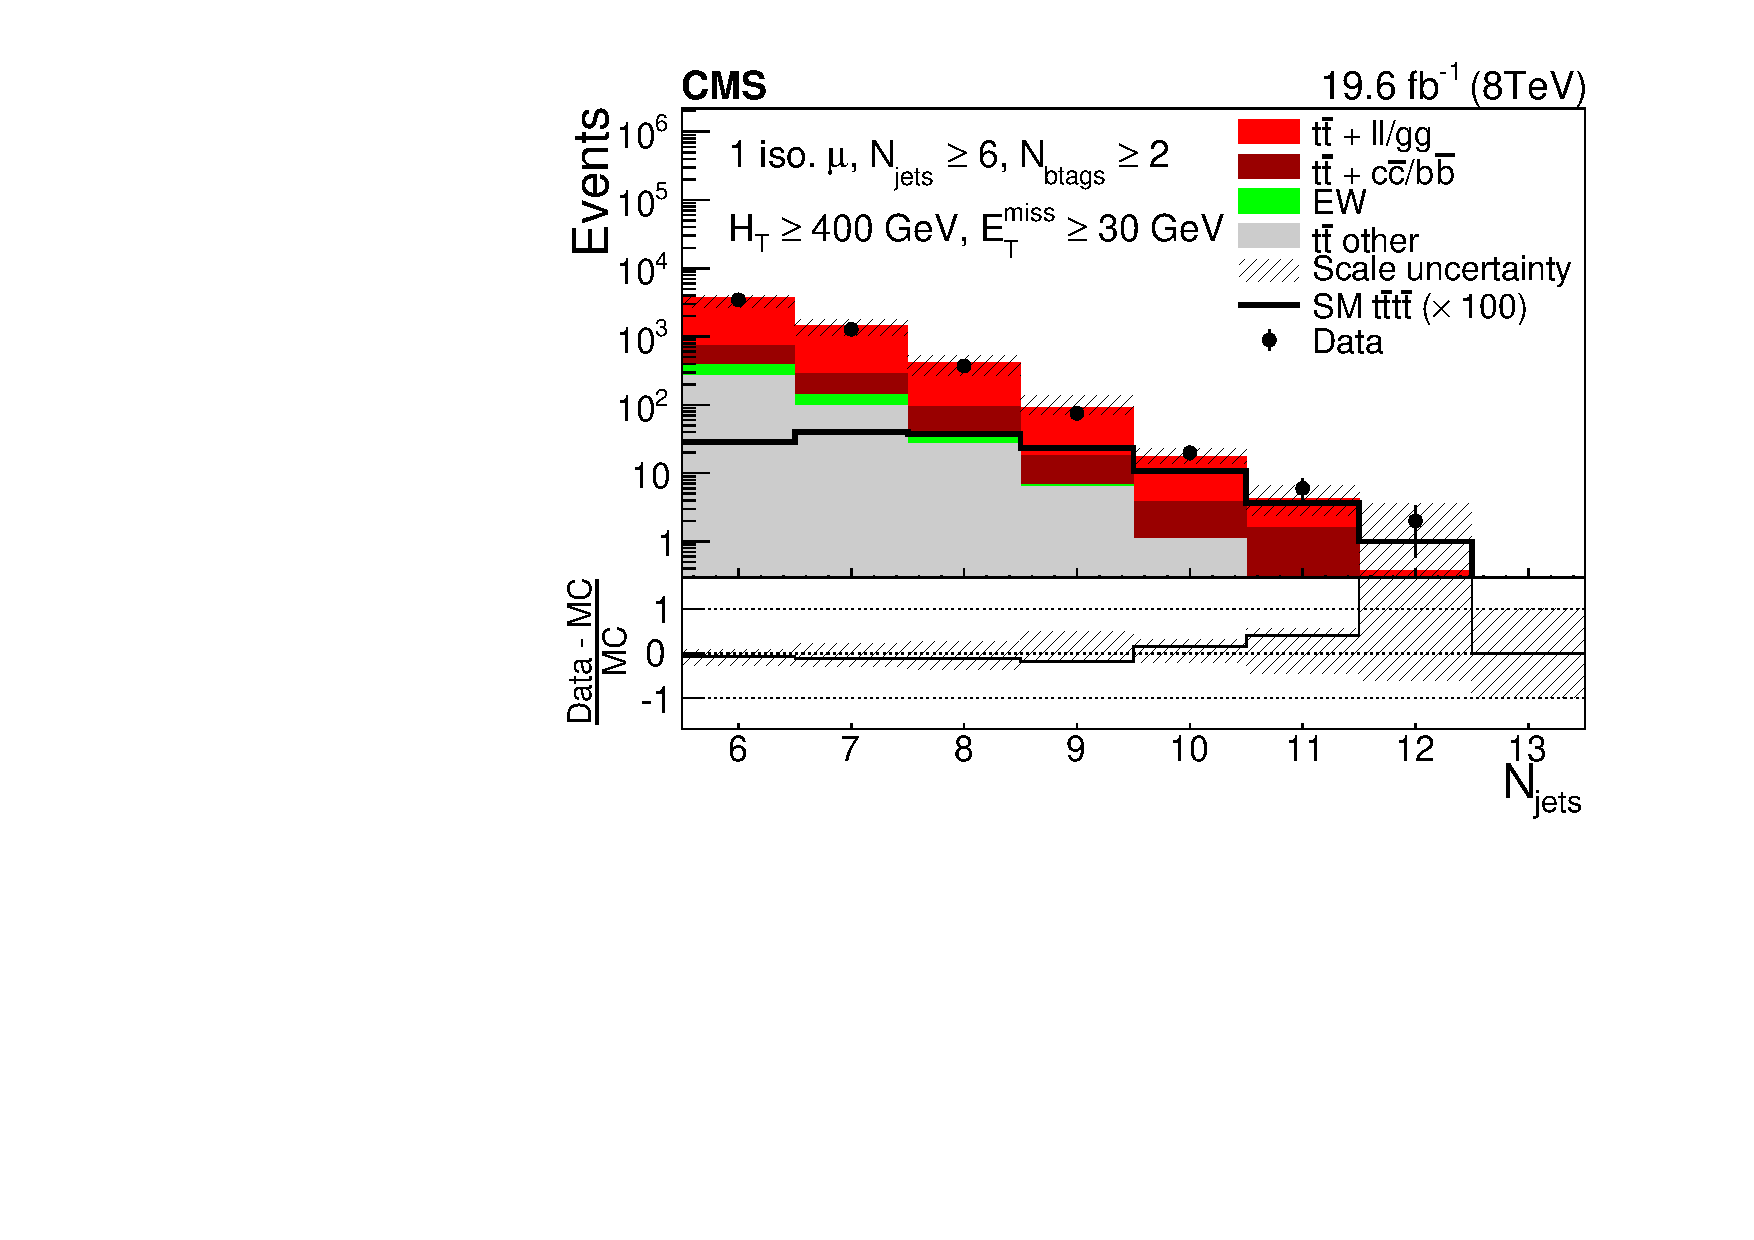
\includegraphics[width=0.49\textwidth]{images/Run1/figures/NbOfSelectedJets_mu.pdf}
     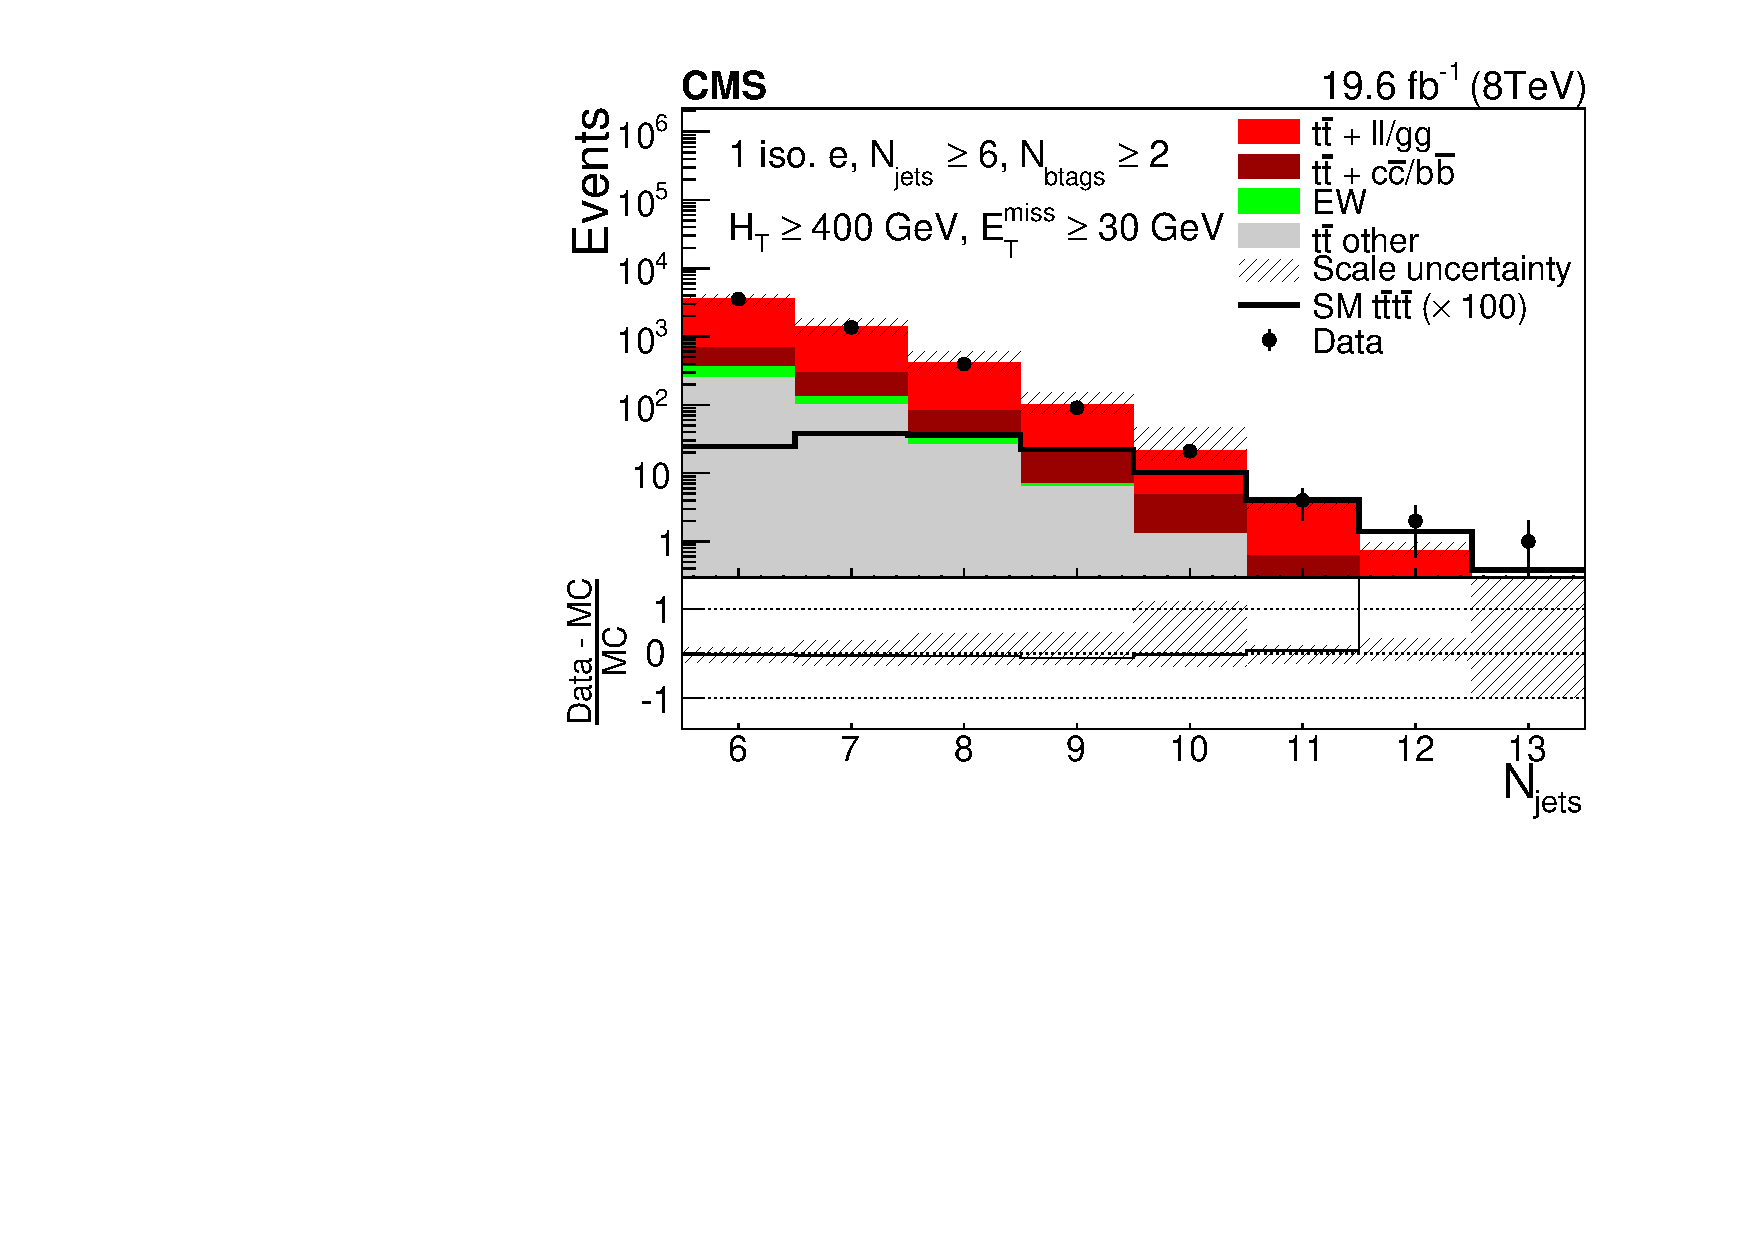
\includegraphics[width=0.49\textwidth]{images/Run1/figures/NbOfSelectedJets_e.pdf}       
    \caption{Distribution of \njets after selection for $\mu$ + jets (right) and e + jets (left).}
    \label{fig:datasimnjets}
\end{figure}

\begin{figure}[ht!]
\centering
    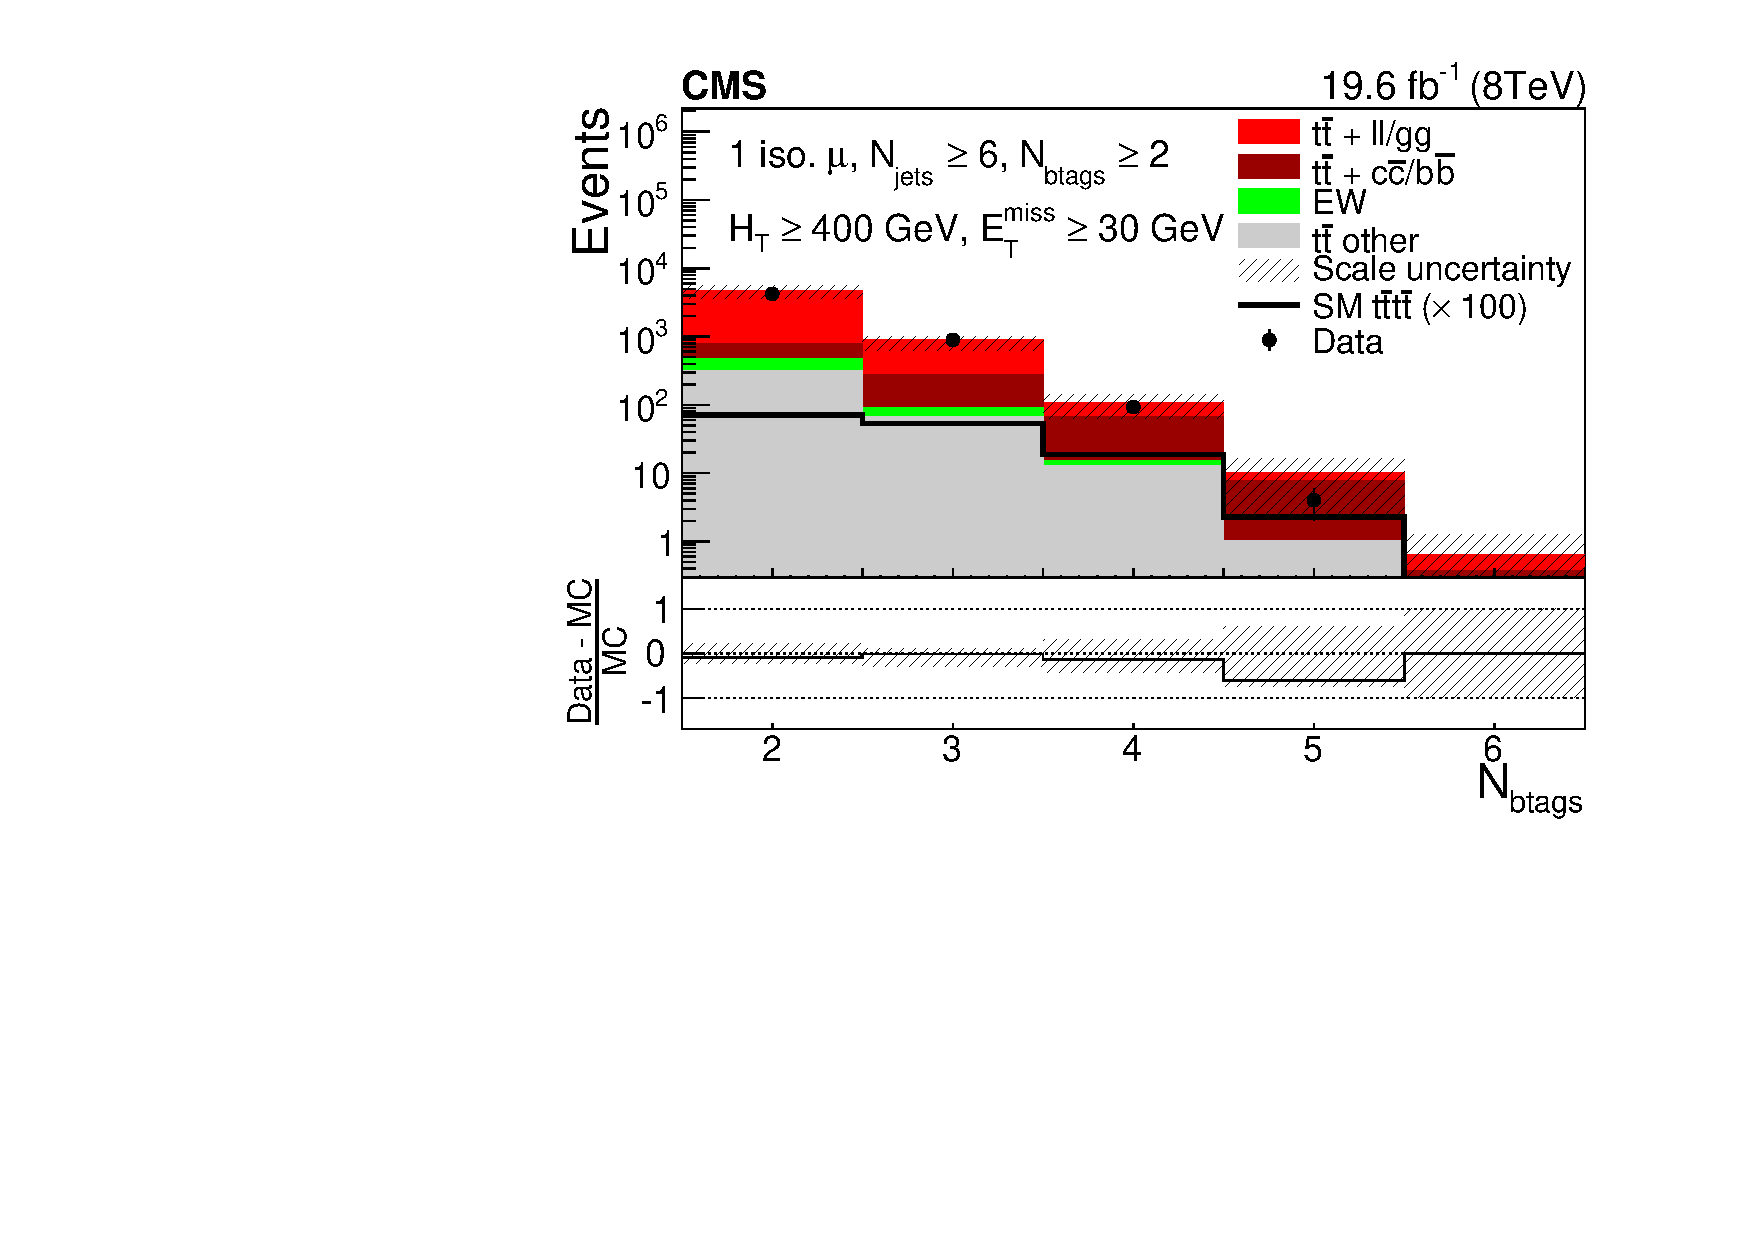
\includegraphics[width=0.49\textwidth]{images/Run1/figures/NbOfSelectedBJets_mu.pdf}
     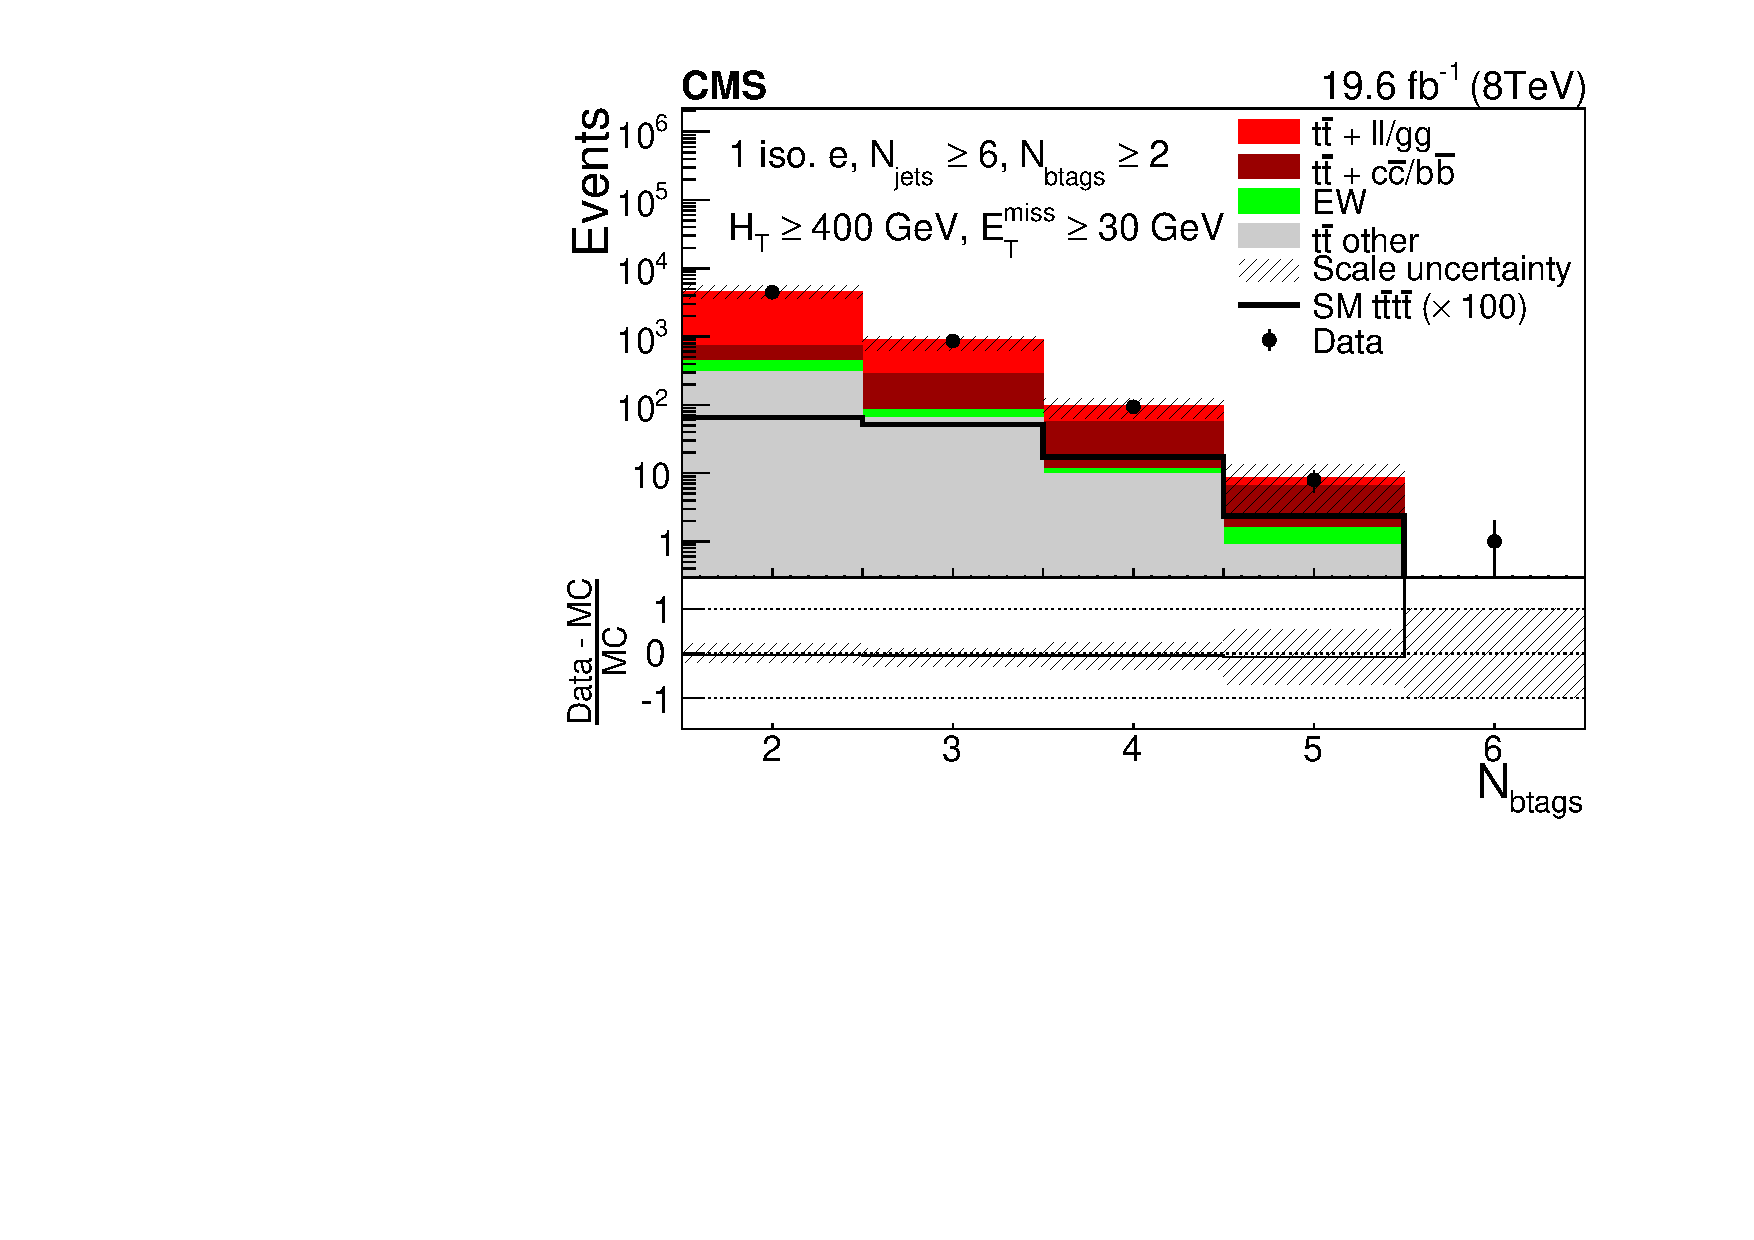
\includegraphics[width=0.49\textwidth]{images/Run1/figures/NbOfSelectedBJets_e.pdf}        
    \caption{Distribution of \nbtags after selection for $\mu$ + jets (right) and e + jets (left).}
    \label{fig:datasimnbtags}
\end{figure}

\begin{figure}[ht!]
\centering
    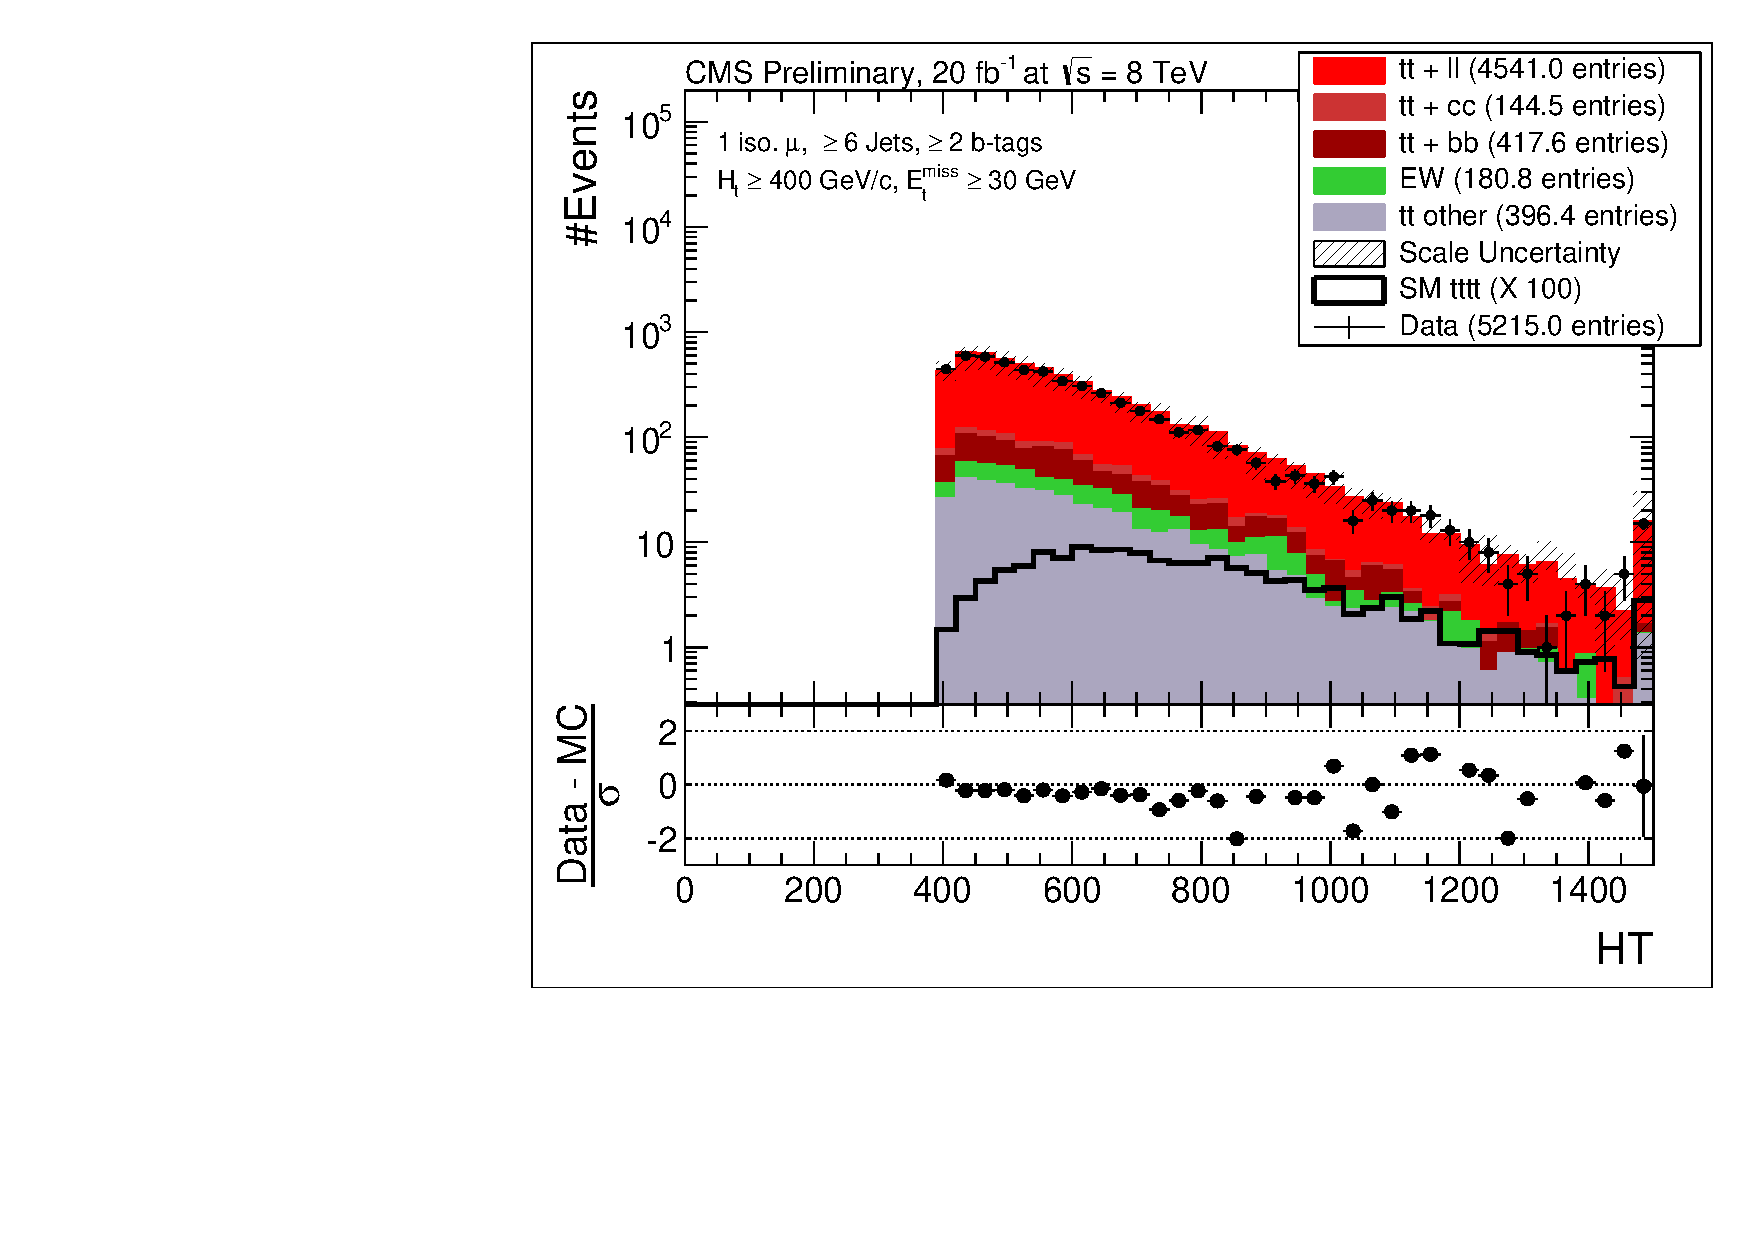
\includegraphics[clip, trim=0.15cm 0.15cm 0.15cm 0.1cm, width=0.49\textwidth]{images/Run1/HT_SelectedJets_StackLogY_Mu.pdf}
     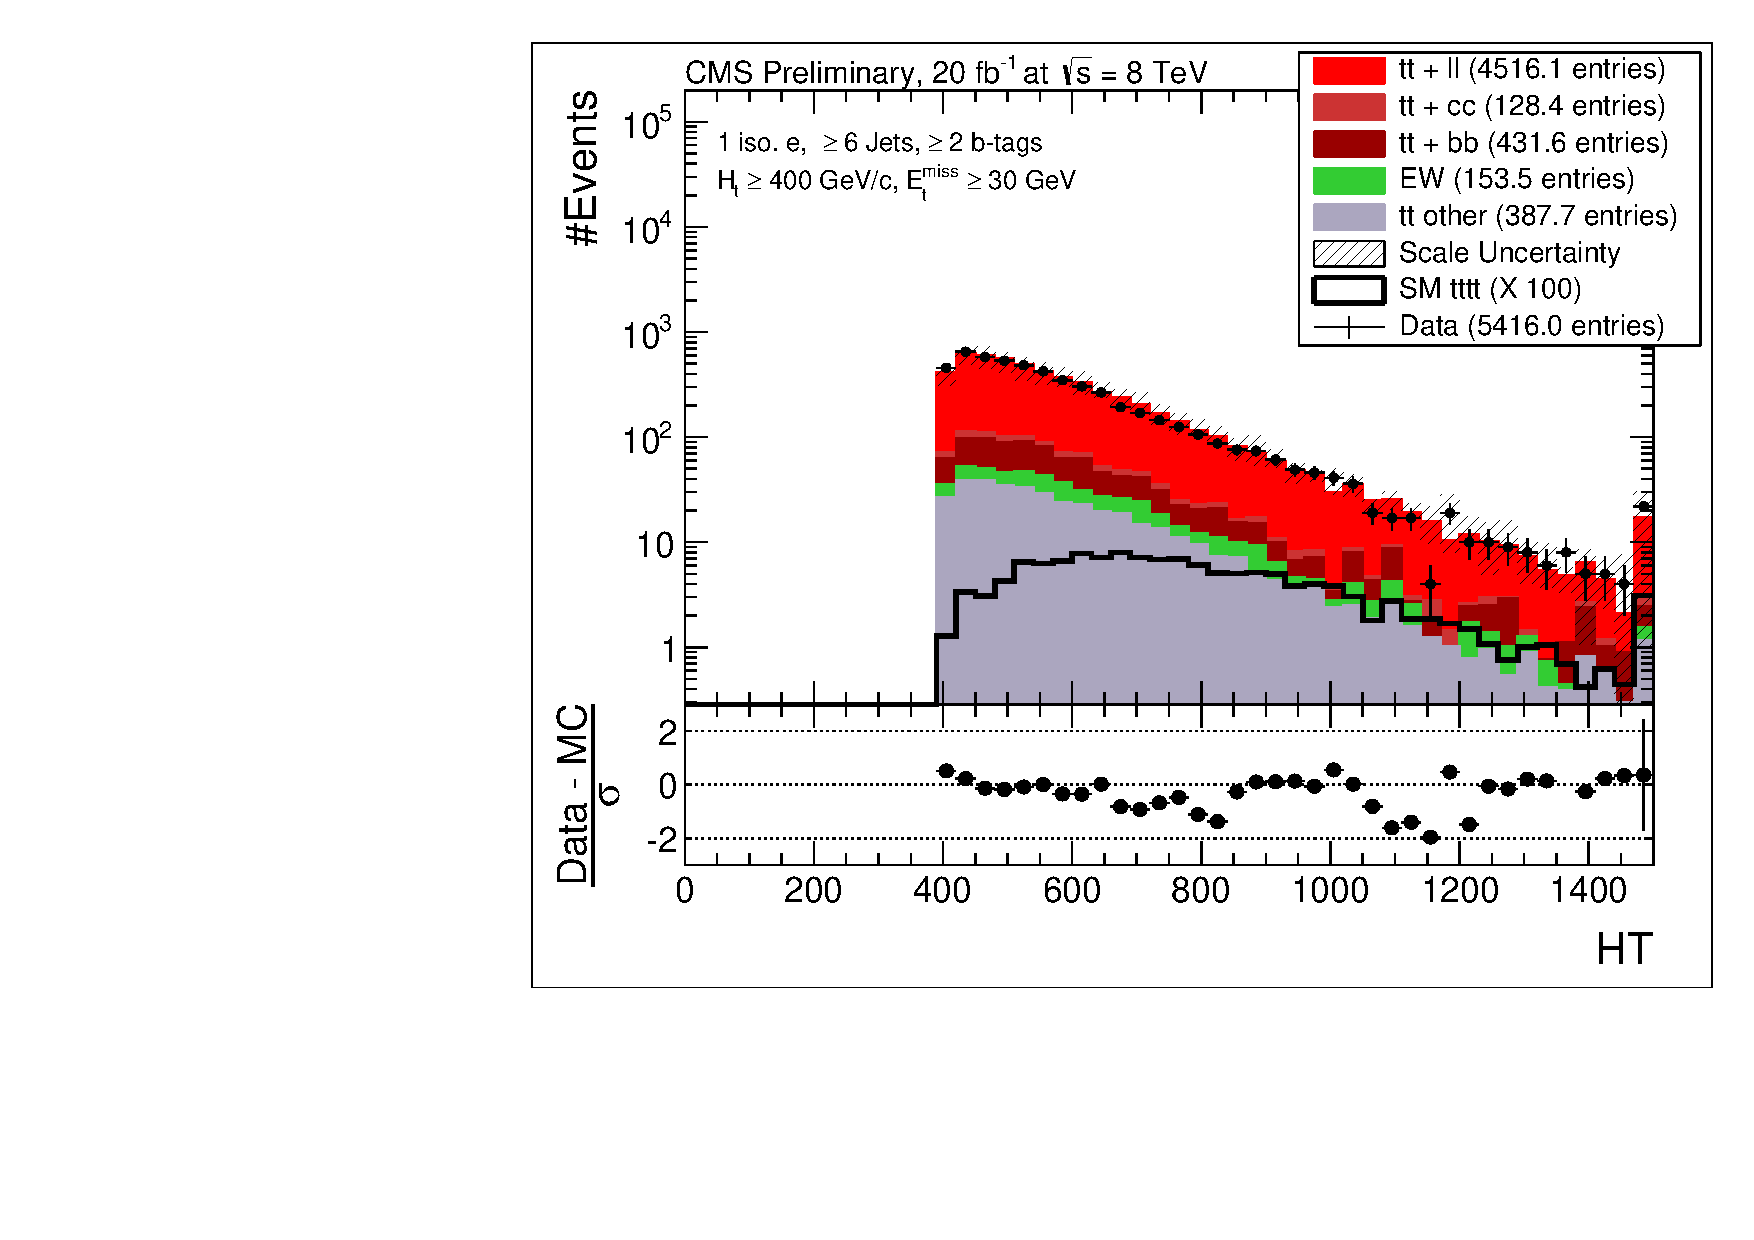
\includegraphics[clip, trim=0.15cm 0.15cm 0.15cm 0.1cm, width=0.49\textwidth]{images/Run1/HT_SelectedJets_StackLogY_e.pdf}          
    \caption{Distribution of \HT after selection for $\mu$ + jets (right) and e + jets (left). }
    \label{fig:datasimHT}
\end{figure}

\begin{figure}[ht!]
\centering
    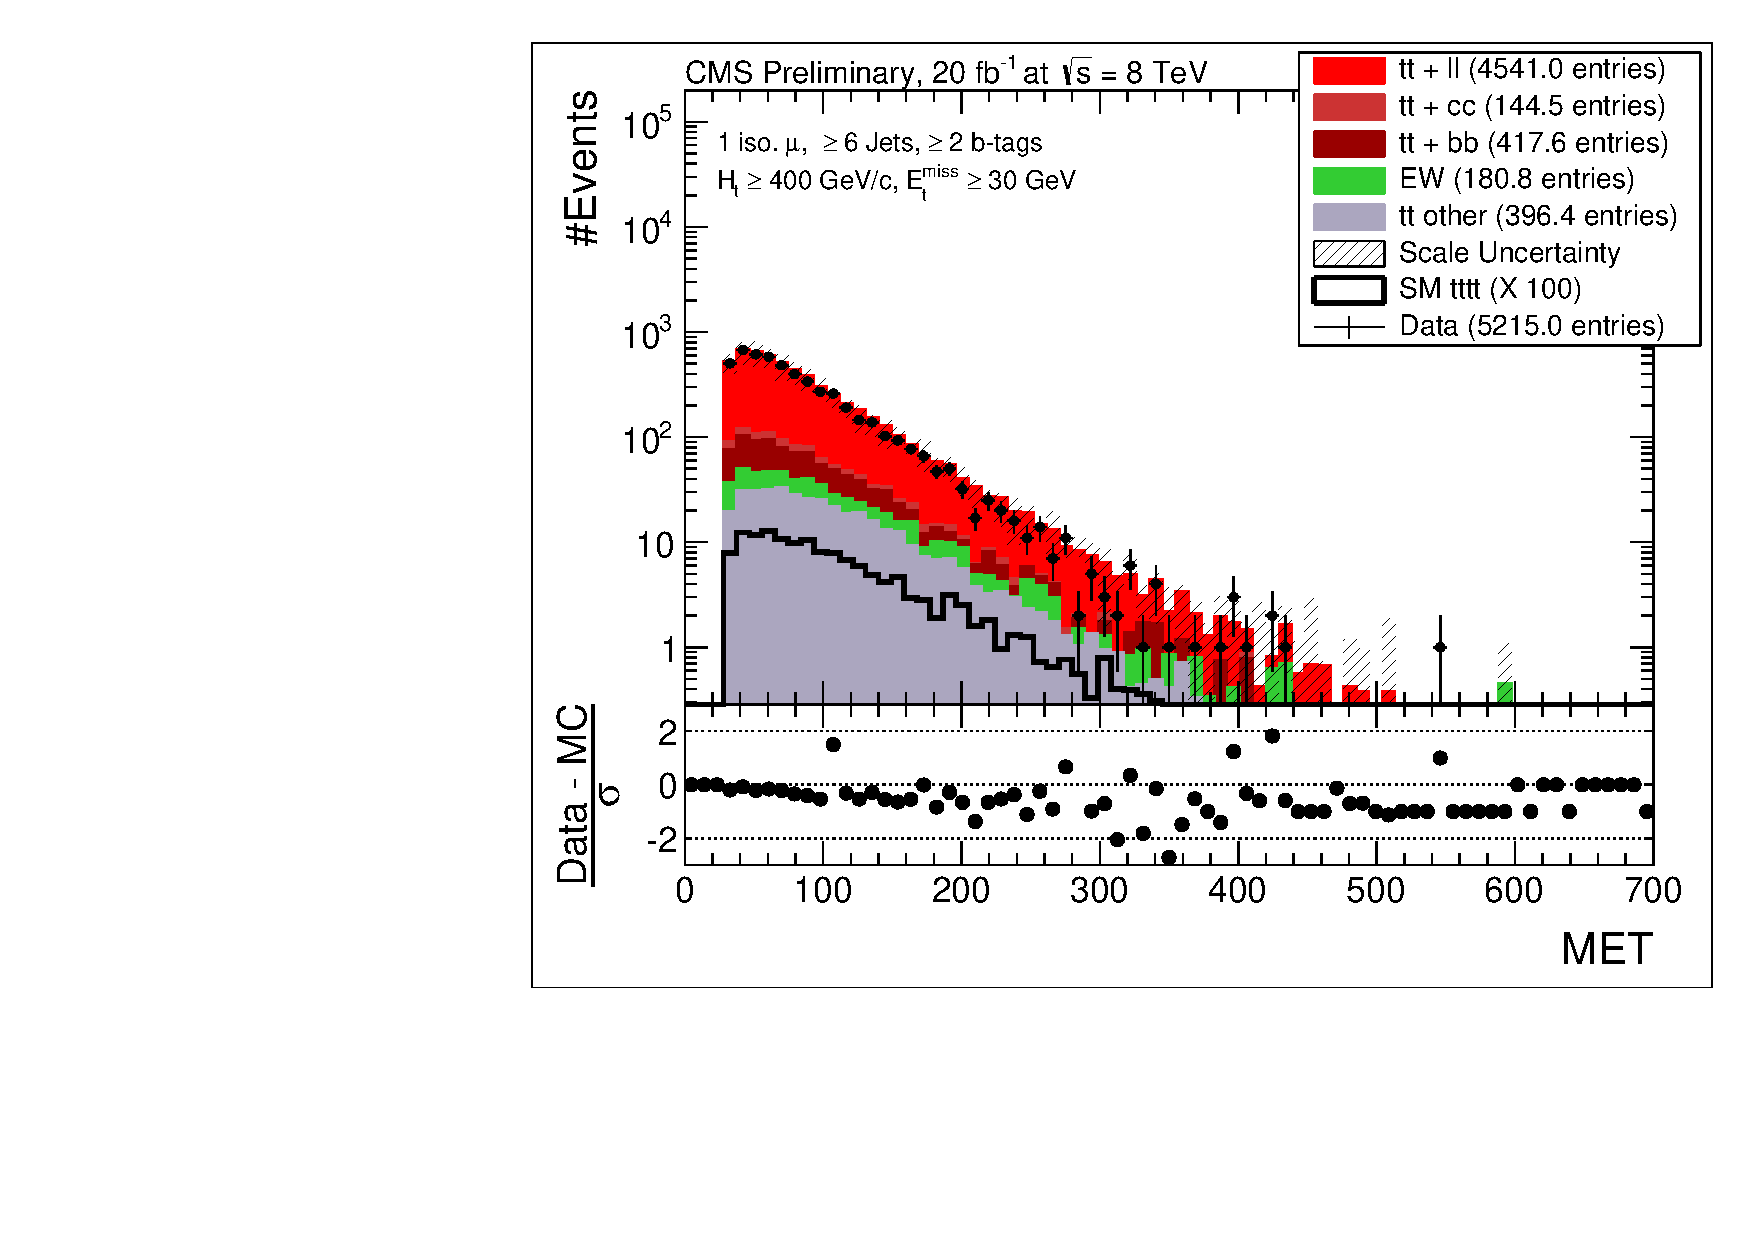
\includegraphics[clip, trim=0.15cm 0.15cm 0.15cm 0.1cm, width=0.49\textwidth]{images/Run1/MET_StackLogY_Mu.pdf}
     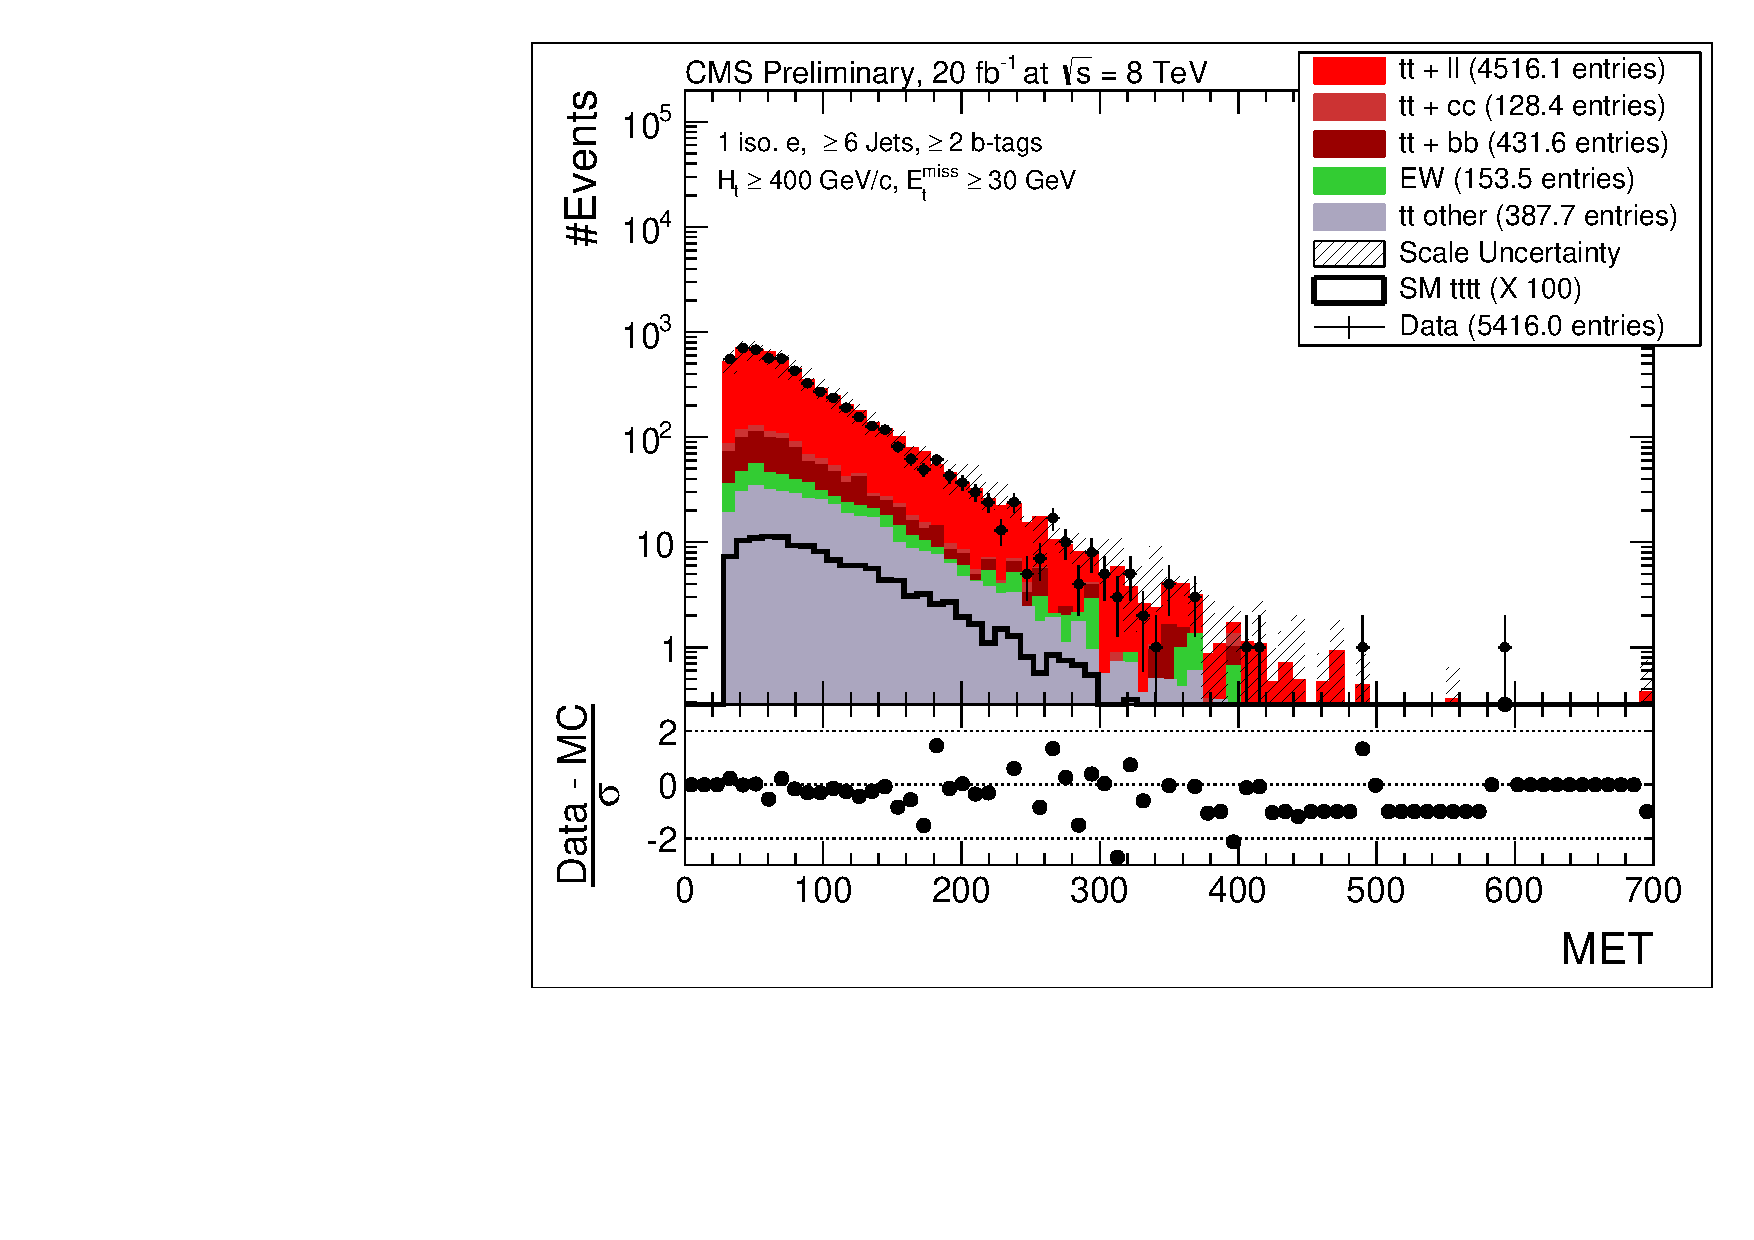
\includegraphics[clip, trim=0.15cm 0.15cm 0.15cm 0.1cm, width=0.49\textwidth]{images/Run1/MET_StackLogY_e.pdf}          
    \caption{Distribution of \MET after selection for $\mu$ + jets (right) and e + jets (left). }
    \label{fig:datasimMET}
\end{figure}



\section{Multi-jet background estimation}
\label{sec:QCDbackground}
The presence of multi-jet events within the signal region defined by the baseline selection is investigated in this section. 
%It is rare for multi-jet events to have a highly energetic undetectable particle. Therefore, the $\MET$ distributions for multi-jet events typically peak at \fxnote*{more specific?}{low values}. 
It can be seen from the MET distributions in Fig.~\ref{fig:datasimMET} that the data agrees well with the simulation at low values which suggests there are very few multi-jet events which pass the tight requirements in the baseline selection. 
%Due to this small number of events, it is not possible to use multi-jet MC to estimate this background. In this case, a data-driven method known as the \fxnote*{ref?}{ABCD method} may be used. This method proceeds by selecting two uncorrelated variables from the object or baseline selection and defining three control regions (A,B,C) and one signal region (D) in the 2-dimensional phase space of these variables. The event variable \MET and the lepton variable RelIso were selected as they are \fxnote*{uncorrelated proof??}{uncorrelated} and 
The data-driven ABCD method, which is described in Section~\ref{sec:QCDbackground}, is used to estimated the multi-jet background. The defined regions in the uncorrelated variables of \MET and $RelIso$ are shown below. The upper bound in $RelIso$ is restricted by the minimum $RelIso$ values required by the HLT in the single muon and single electron data sets.\\

For the muon channel these are:
\begin{itemize}
\setlength\itemsep{0em}
\item A : 30 $<\MET<$ 500, 0.1 $<$ RelIso $<$ 0.15
\item B : 0 $<\MET<$ 30, 0.1 $<$ RelIso $<$ 0.15
\item C : 0 $<\MET<$ 30, 0 $<$ RelIso $<$ 0.1
\item D : 30 $<\MET<$ 500, 0 $<$ RelIso $<$ 0.1
\end{itemize}
For the \eplusjets:
\begin{itemize}
\itemsep0em
\item A : 30 $<\MET<$ 500, 0.12 $<$ RelIso $<$ 0.2
\item B : 0 $<\MET<$ 30, 0.12 $<$ RelIso $<$ 0.2
\item C : 0 $<\MET<$ 30, 0 $<$ RelIso $<$ 0.12
\item D : 30 $<\MET<$ 500, 0 $<$ RelIso $<$ 0.12
\end{itemize}

%It is assumed that the multi-jet background can be estimated from the data minus the background expectation from all of the other MC samples considered in Section~\ref{sec:datasimulation}. 
The results of the background subtraction from data and the defined ABCD regions are shown in Fig.~\ref{fig:QCDplots}.
The number of multi-jet events, N$_{\textrm{multi-jet}}$, in each of the control regions are used to predict the number of multi-jet events in region D using Eq.~\ref{N-multi-jet}, the results of which are shown in Table~\ref{tab:multijet}.

\begin{figure}[!ht]
    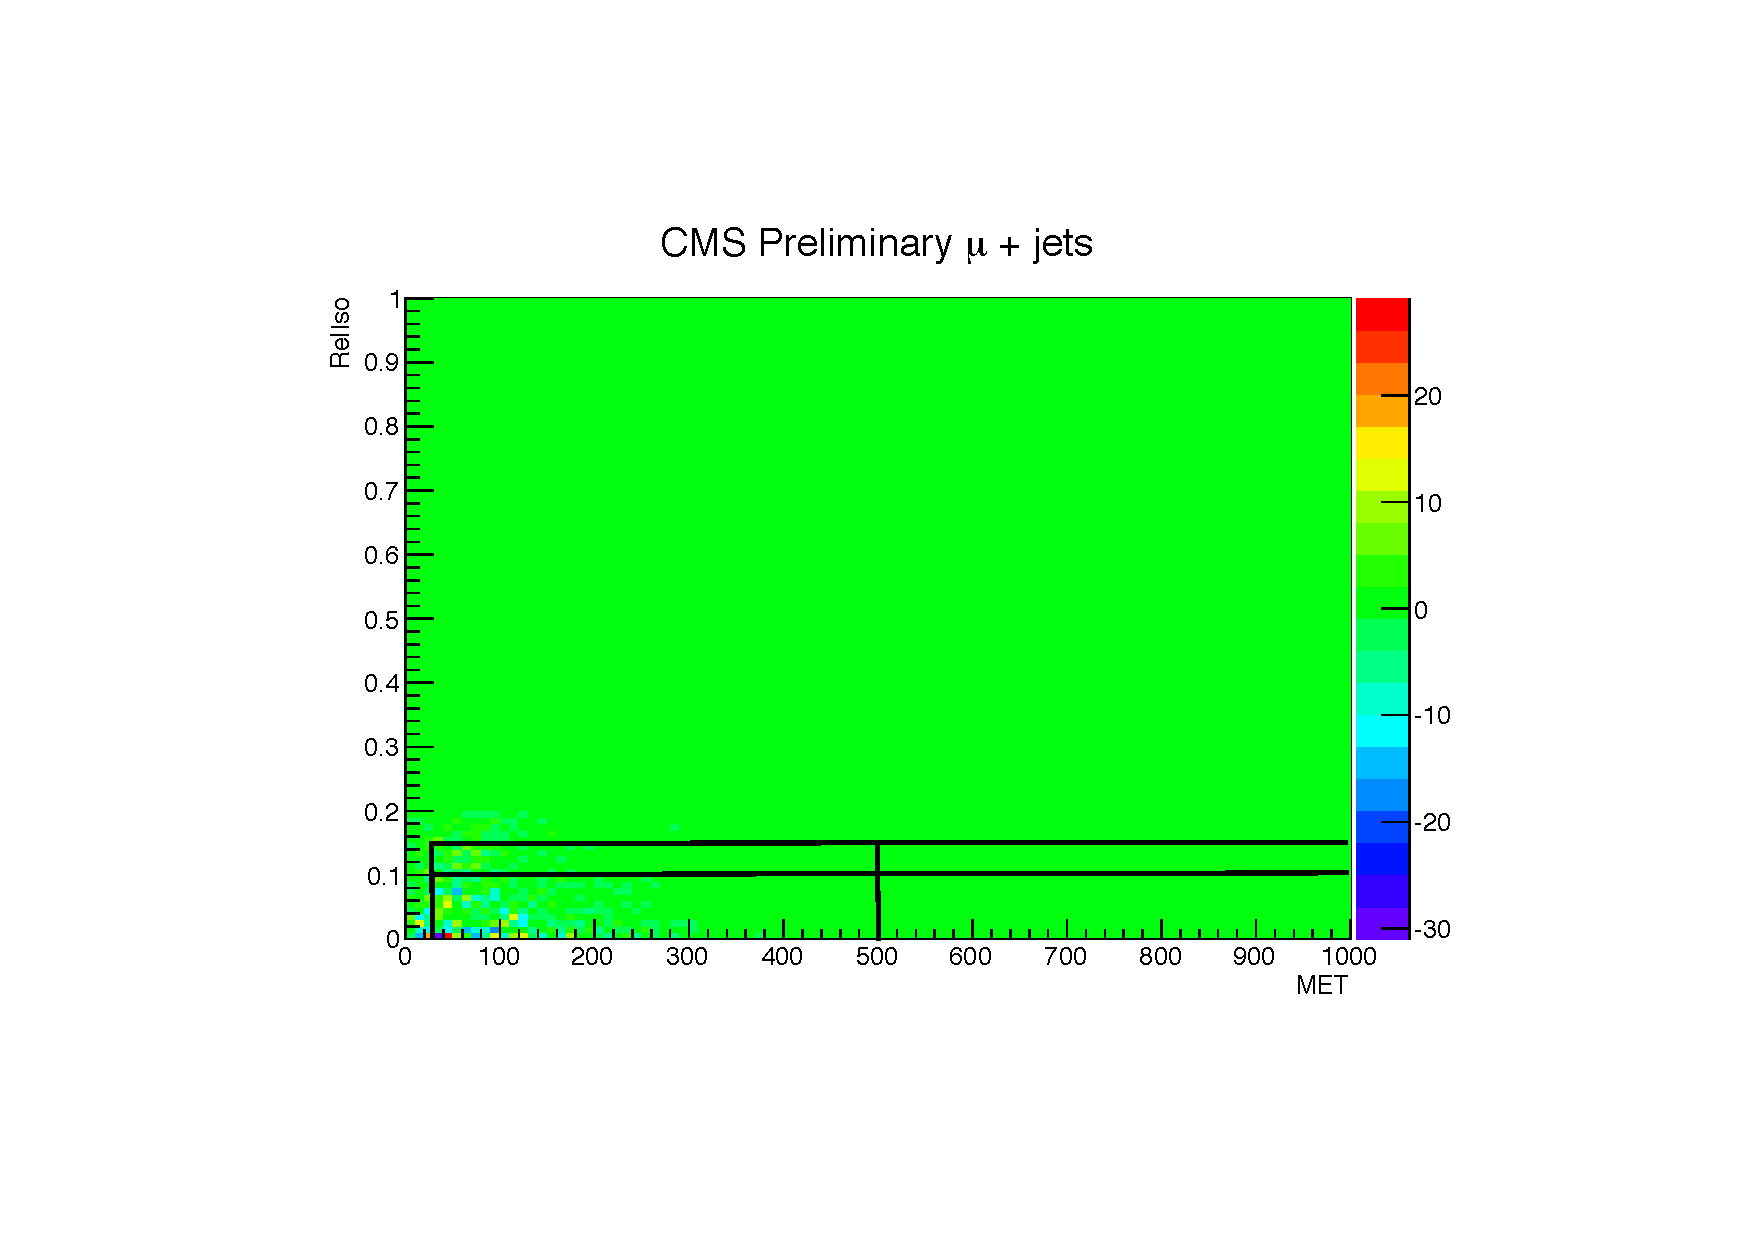
\includegraphics[width=0.49\textwidth]{images/Run1/Data_Minus_MC_Mu_Lines2.pdf}
    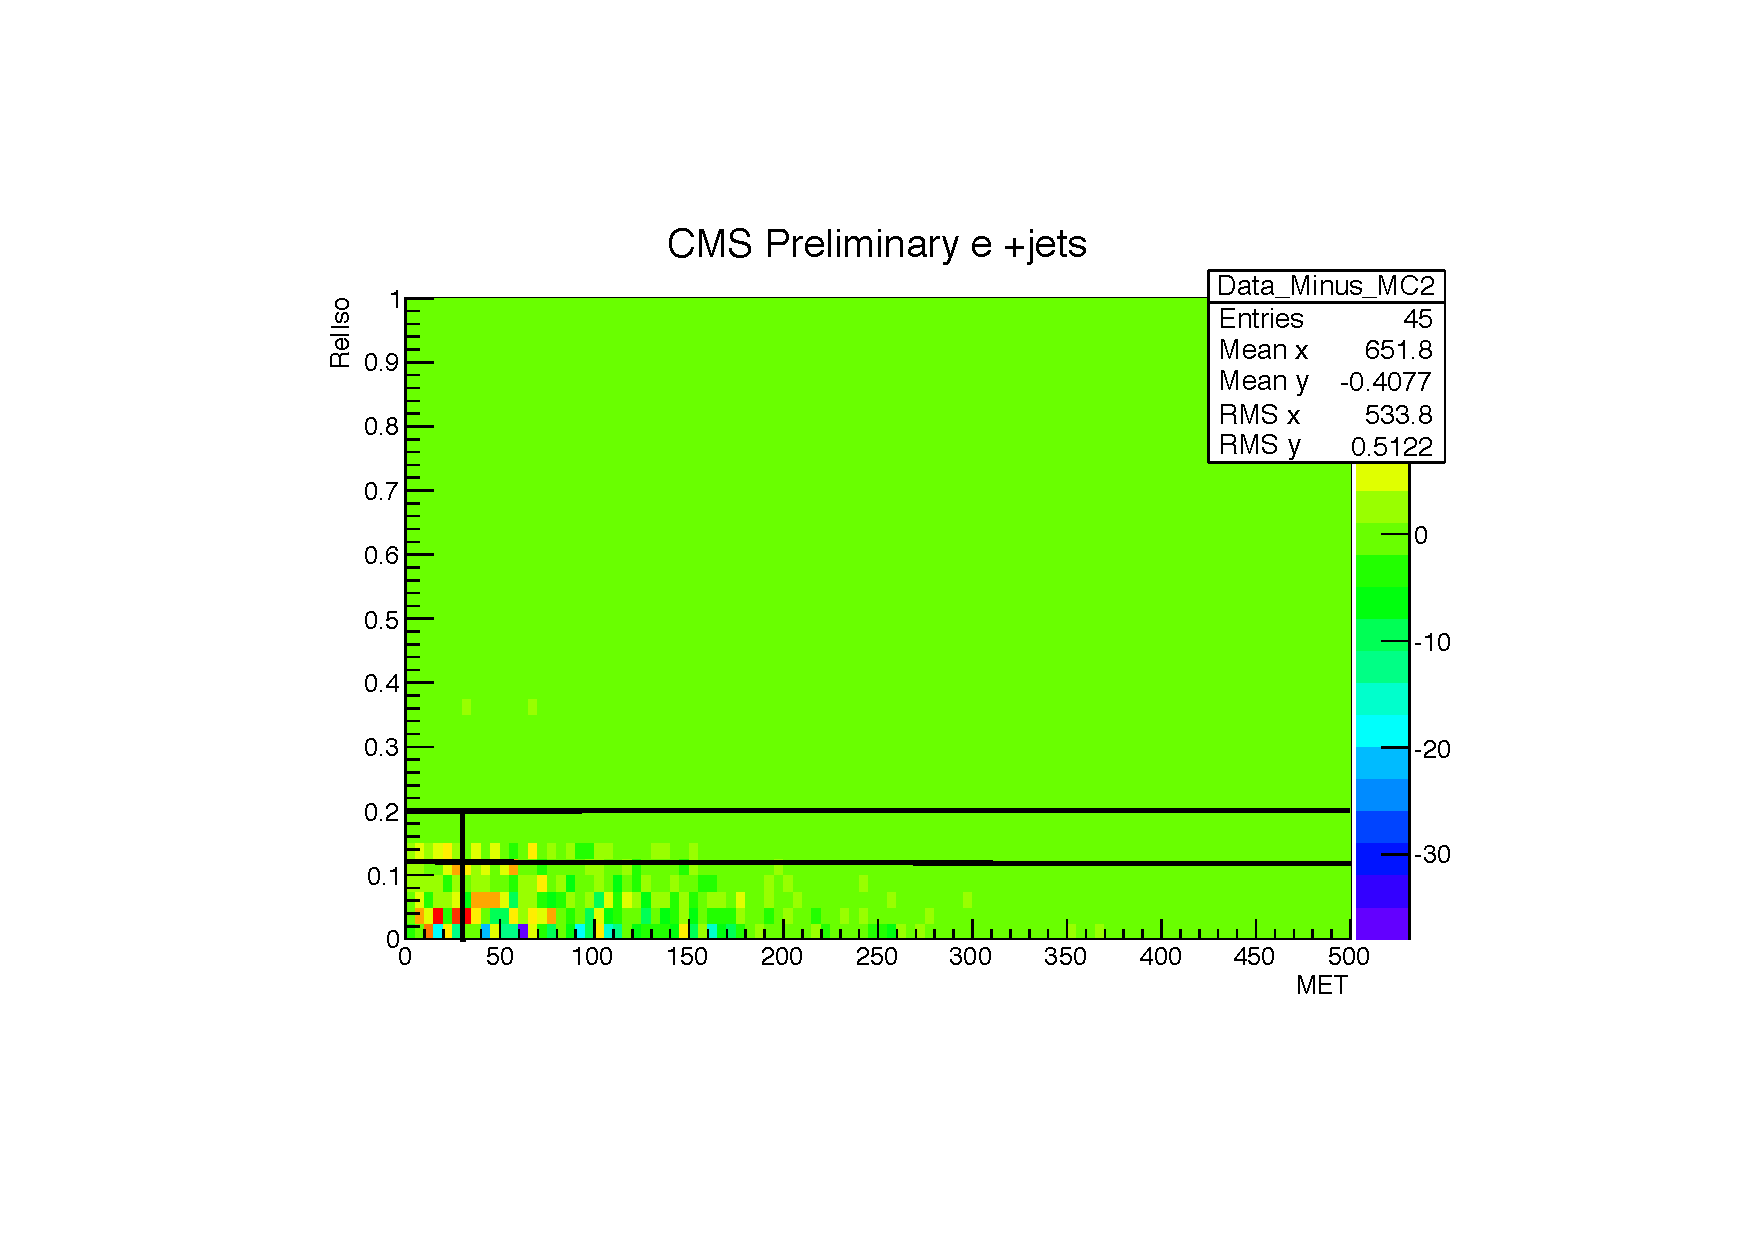
\includegraphics[width=0.49\textwidth]{images/Run1/Data_Minus_MC_El_Lines2.pdf}
    \caption{Number of events after selection requirements and background subtraction for $\mu$ + jets (right) and e + jets (left).}
    \label{fig:QCDplots}
\end{figure}


\begin{equation}
\frac{\textrm{N}^{\textrm{B}}_{\textrm{multi-jet}}}{\textrm{N}^{\textrm{A}}_{\textrm{multi-jet}}} = \frac{\textrm{N}^{\textrm{C}}_{\textrm{multi-jet}}}{\textrm{N}^{\textrm{D}}_{\textrm{multi-jet}}}
\label{N-multi-jet}
\end{equation}

\begin{table}[ht!]
\caption{Multi-jet estimation}
\centering
\begin{tabular}{|c |c |c |c |c |}
 \hline 
 Channel & N$^{\textrm{A}}_{\textrm{multi-jet}}$  & N$^{\textrm{B}}_{\textrm{multi-jet}}$ & N$^{\textrm{C}}_{\textrm{multi-jet}}$ & Prediction for N$^{\textrm{D}}_{\textrm{multi-jet}}$  \\
  \hline
$\mu$ + jets & 19.1 & 16.1 & -16.8 & -20  \\
 \hline
$e$ + jets & 36.8  & 50.8 & 62.7 &45.5  \\
\hline
\end{tabular}
\label{tab:multijet}
\end{table}

As the number of \ttbar events in simulation has fluctuated to be greater than the data in region C in the muon channel, the prediction for the signal region D is negative. As this prediction is unphysical, the number of events is estimated to be zero in the muon channel. In the electron channel, 45.5 multi-jet events are predicted which is considered negligible at $<1\%$ of the large \ttbar background. Hence, the multi-jet background is not considered further.
% \fxnote{scale up scale down...200\% uncertainty?}

\section{Discriminating between signal and background}
\label{sec:discriminating}
As seen from the tables in section~\ref{cutflow}, the dominant background process after the baseline selection is \ttbar production, which is three orders of magnitude greater than \tttt production in the signal region.
In this section, details of the hadronic top quark reconstruction (described in section~\ref{sec:topreco}) and the variables that can be defined from the output of this MVA will be discussed as well as the variables which are used in the event-level BDT.

% This motivates the search for variables which can discriminate between these two processes.
There are three categories of observables which are used to discriminate: the number of top quarks which can be reconstructed in the event, the number of b-jets found in each event, and event activity such as \HT.

\subsection{Hadronic top quark content}
\label{sec:topContent}
% In the single lepton channel for \tttt production, there are three top quarks where the W boson decays hadronically, these will be referred to as hadronic top quarks. For the main background of \ttbar there is only one hadronic top quark. Additional jets in \ttbar come from \fxnote*{assume previously defined}{ISR or FSR} in order to satisfy the requirements of the baseline selection. Therefore, it should only be possible to reconstruct more than one top quark from three jets originating from it's hadronic decay in \tttt but not in \ttbar. However, 

The \antikt algorithm can only distinguish separate jets if they are separated by \DR$>0.5$, hence it may not always be possible to reconstruct all hadronic top quarks. To ascertain whether it is feasible to use the hadronic top reconstruction to aid in distinguishing \tttt and \ttbar given this criteria, the number of reconstructible tops in \tttt in \ttbar is investigated. Hadronic top quarks are considered reconstructible at parton level if they decayed into jets with \DR  $>$  0.5. Both \tttt and \ttbar events were analysed where there was one muon with \PT $>$ 26 GeV and exactly 6 jets with \PT $>$ 30 and $\lvert \eta \rvert<$ 2.5.  The number of reconstructible hadronic top quarks for \tttt and \ttbar are shown in Fig.~\ref{fig:ReconHadTops}.

\begin{figure}[!ht]
\centering
    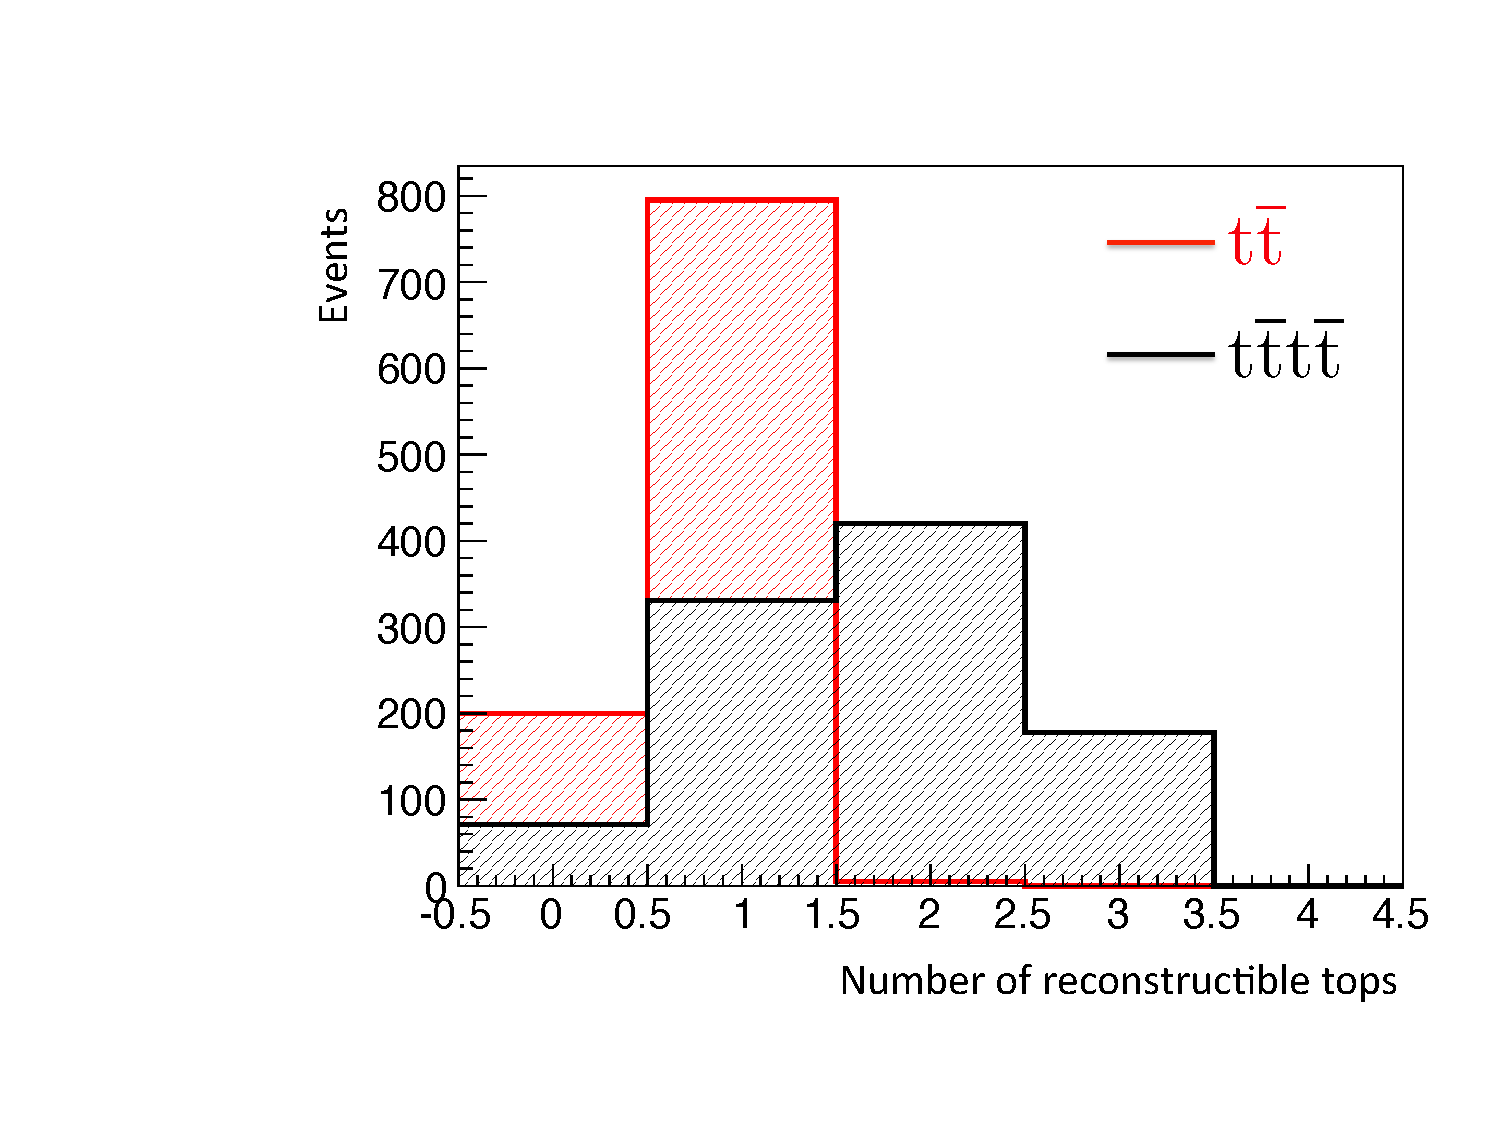
\includegraphics[width=0.6\textwidth]{images/Run1/HadRecoTops.pdf}
    \caption{The number of reconstructible hadronic top quarks in semileptonic \ttbar and \tttt in the single lepton channel.}
    \label{fig:ReconHadTops}
\end{figure}

For \tttt production at parton level it is possible to reconstruct more than one hadronic top quark $\approx$ 63 $\%$ of the time compared to a negligible number of times in \ttbar, as is evident in the Fig.~\ref{fig:ReconHadTops}. Hence, using the number of hadronic tops to distinguish between \tttt and \ttbar is worth investigating. 
% One obstacle to this is the large number of ways in which the jets can be combined in events with \njets $\geq 6$.\fxnote{more on combinatorics? -> but James' work} 

% This motivates the use of multi-variate analysis to distinguish between good tri-jet combinations and bad tri-jet combinations, where a tri-jet refers to any given combination of three jets. Figure~\ref{fig:TopBDTinput} shows the minimal number of discriminating variables which are used including:\\
% \textbf{Tri-jet invariant mass} - Good tri-jet combinations should have an invariant mass distribution which peaks around the top mass.\\
% \textbf{Di-jet invariant mass} - The di-jet combination is formed from the two jets with the smallest \DR separation. The invariant mass distribution should peak around the W mass.\\
% \textbf{\ptrat} - This is the ratio of the vectorial \pt to the scalar sum of the \pt of the jets in the tri-jet combination.\\
% \textbf{\DPTW} - This is the \Dphi separation between the tri-jet and di-jet system.\\
% \textbf{\DPTb} - This is the \Dphi separation between the tri-jet and remaining jet not included in the di-jet system.\\
% \textbf{\CSVj} - For the jet not used in the di-jet system, the CSV b-tagging discriminator value is used.\\

\textbf{BDT}

The variables used in the hadronic top quark reconstruction BDT are shown in Fig.~\ref{fig:TopBDTinput} where it can be seen that the tri-jet and dijet invariant masses provide the most powerful separation. This visualisation can help in finding discriminating variables but it should be considered that the shapes of these distributions will change as the events progress through the BDT where certain events will become more heavily weighted. For instance the $CSV_{j}$ variable appears to not have much separation power initially but the distribution may look quite different in certain areas of phase space or after boosting weights have been applied, and the inclusion of this variable improved the overall separation of the BDT output discriminator.

\begin{figure}[ht!]
\centering
    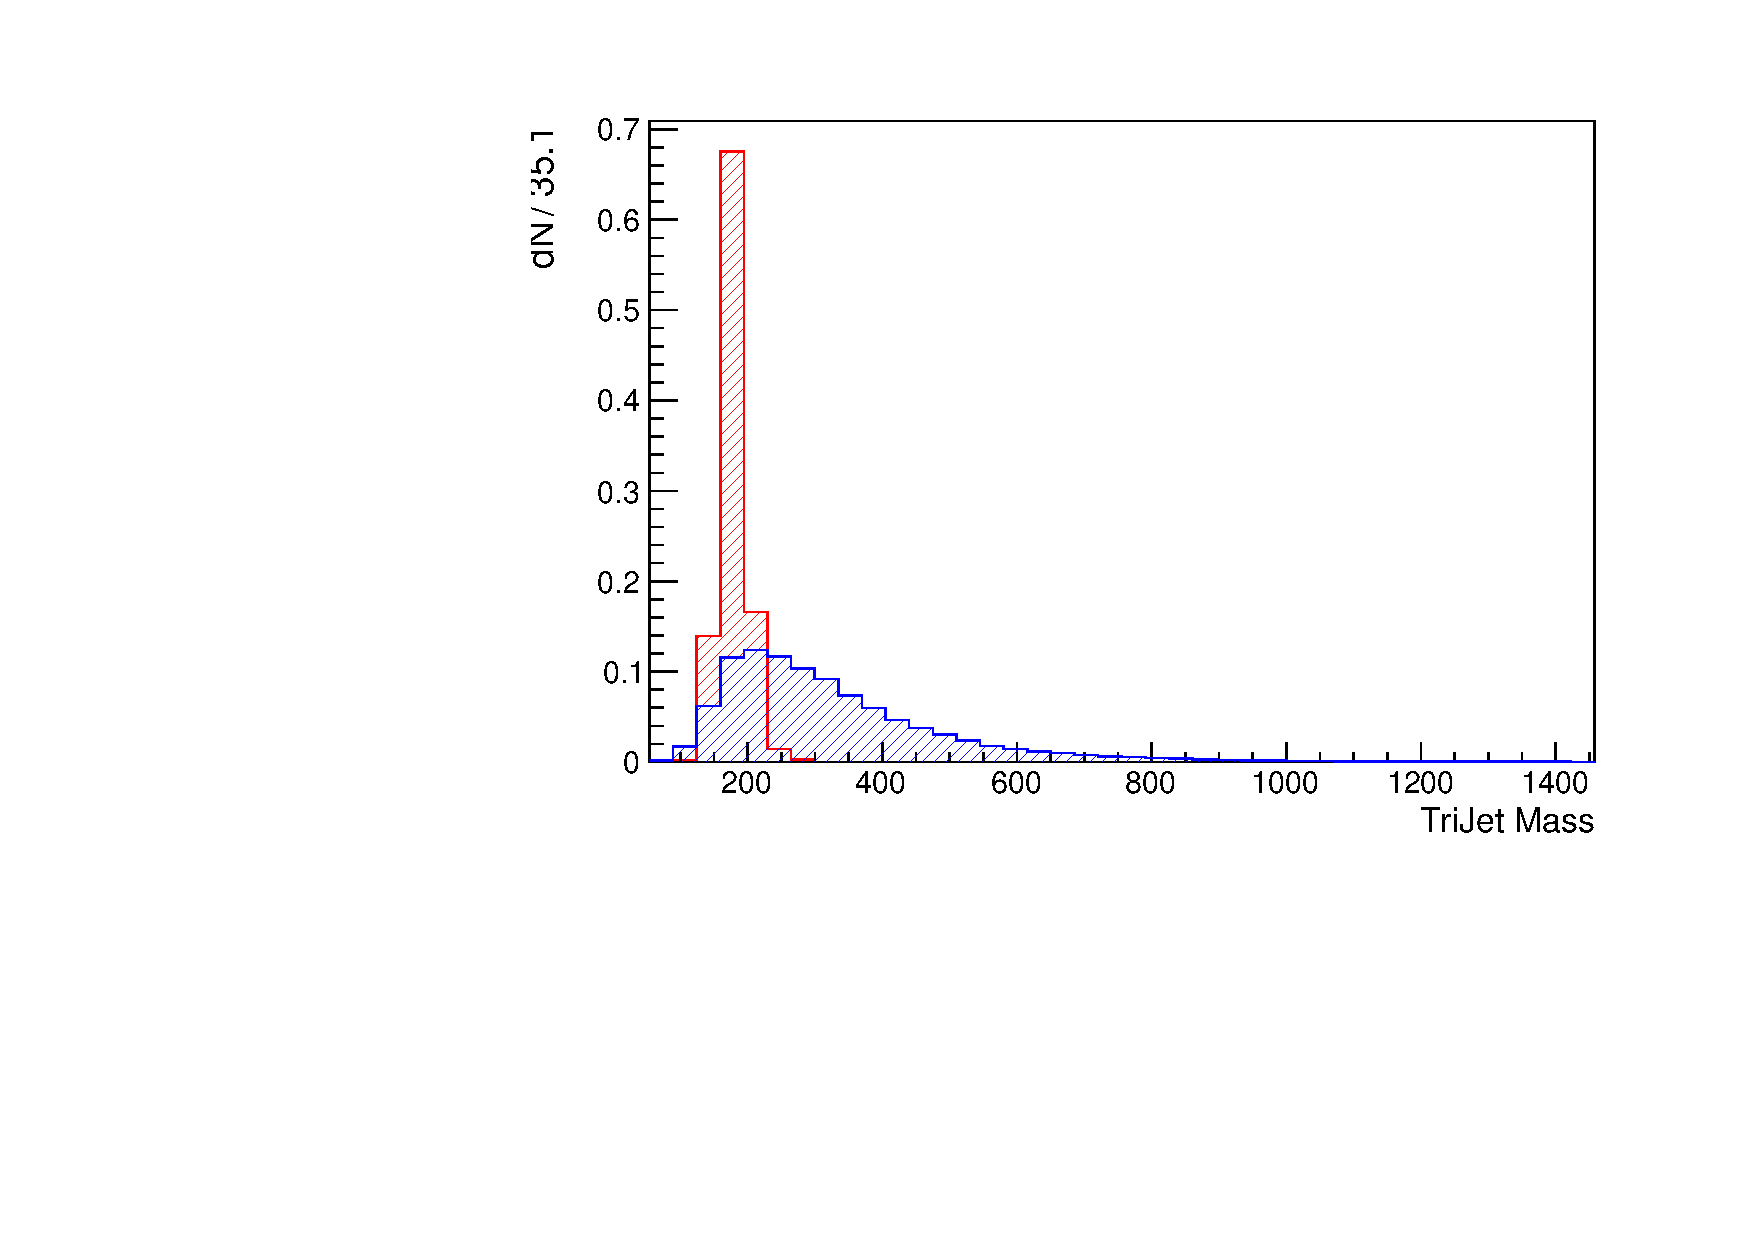
\includegraphics[width=0.49\textwidth]{images/Run1/TriJetMass.pdf}
     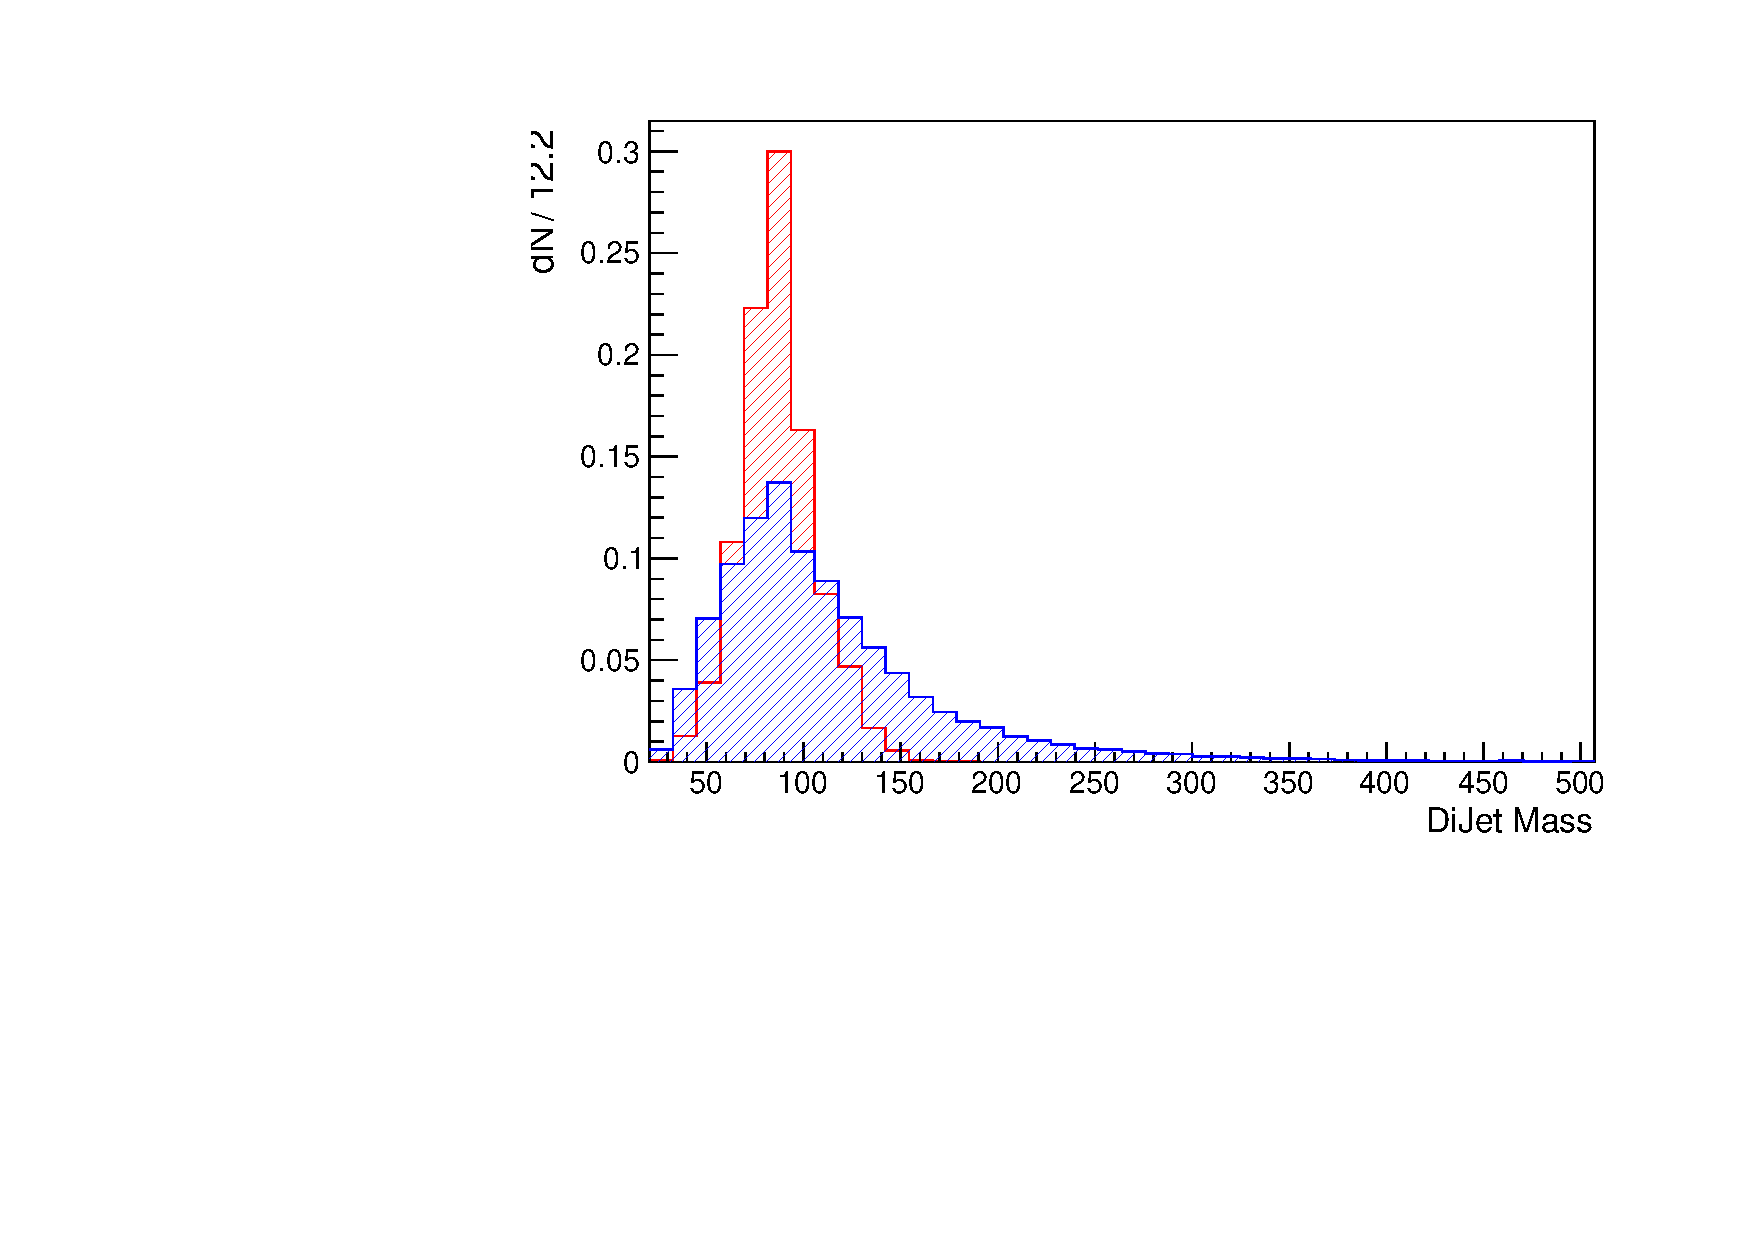
\includegraphics[width=0.49\textwidth]{images/Run1/HadWMass.pdf}
    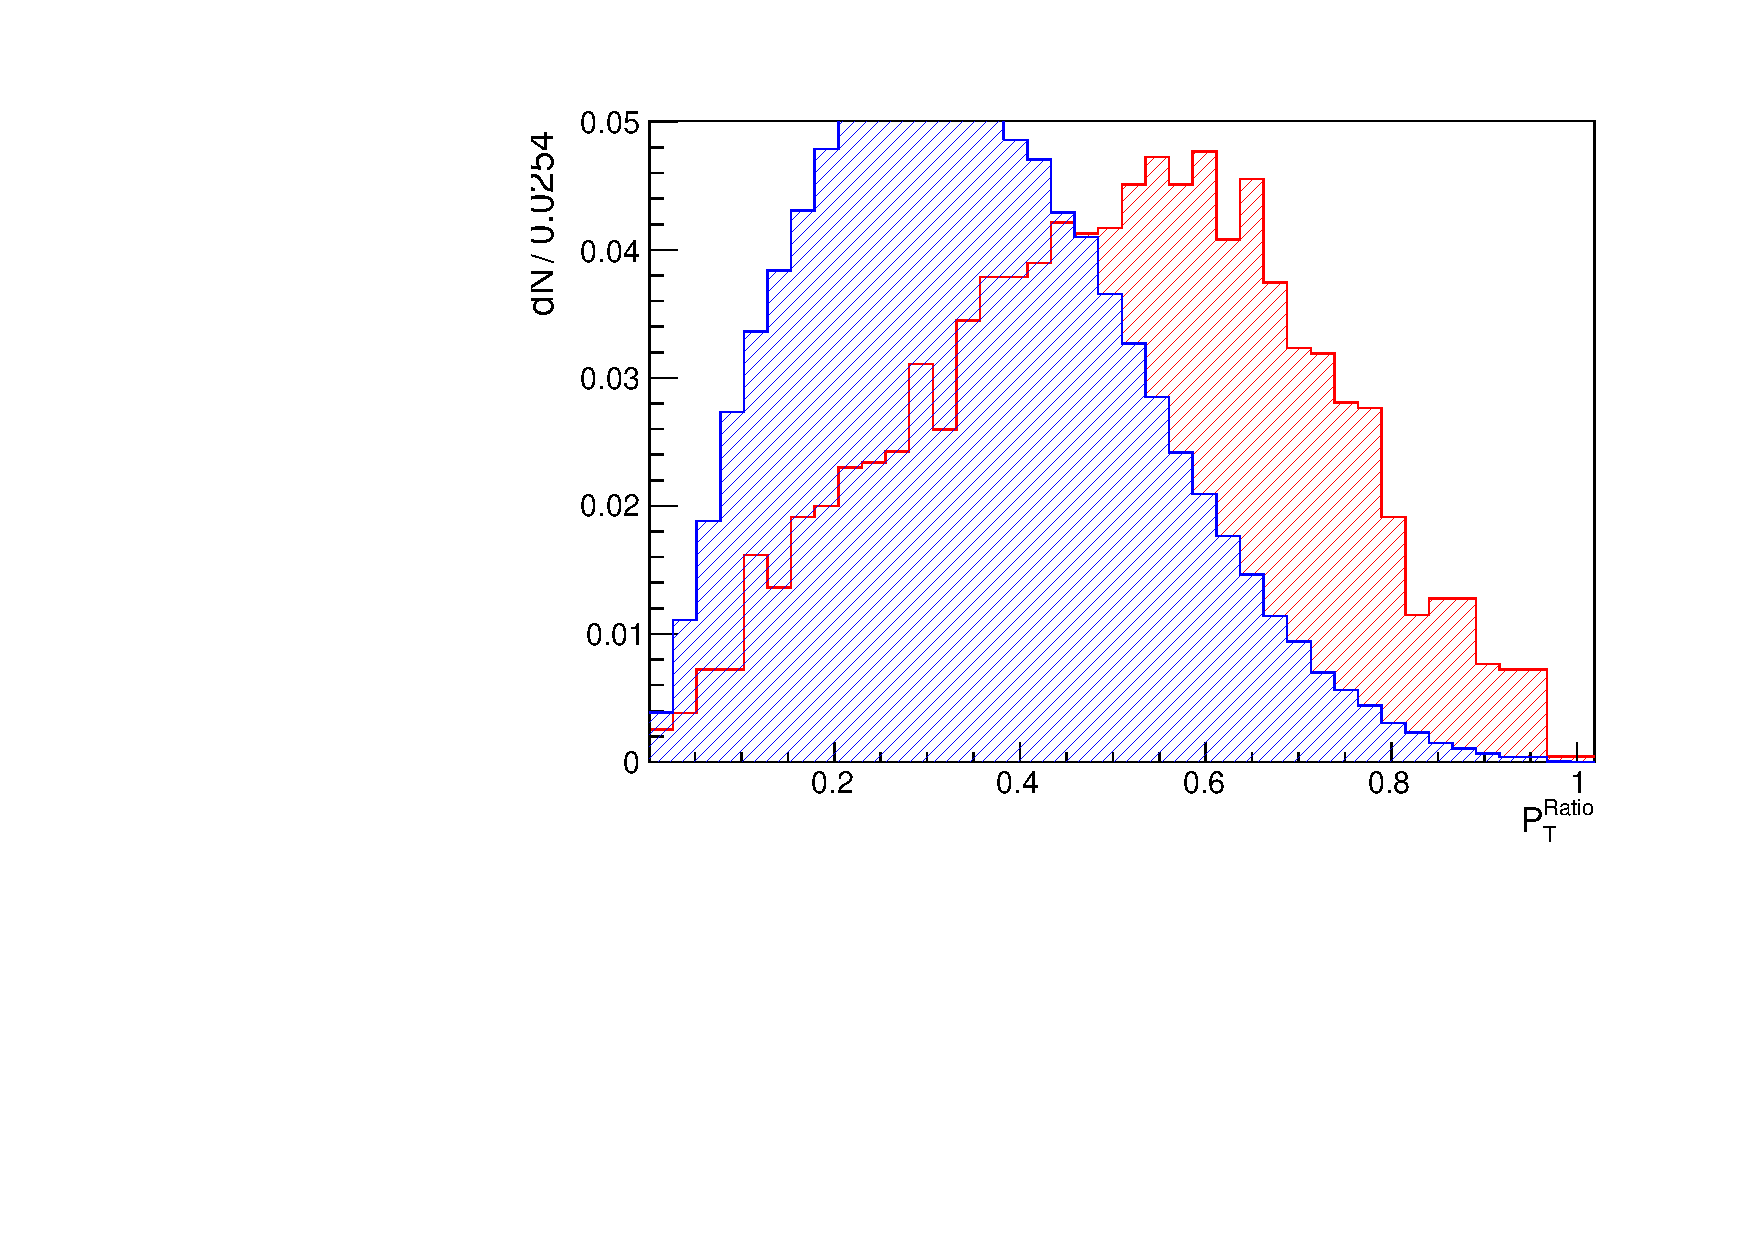
\includegraphics[width=0.49\textwidth]{images/Run1/ThSumPTVecPT.pdf}
     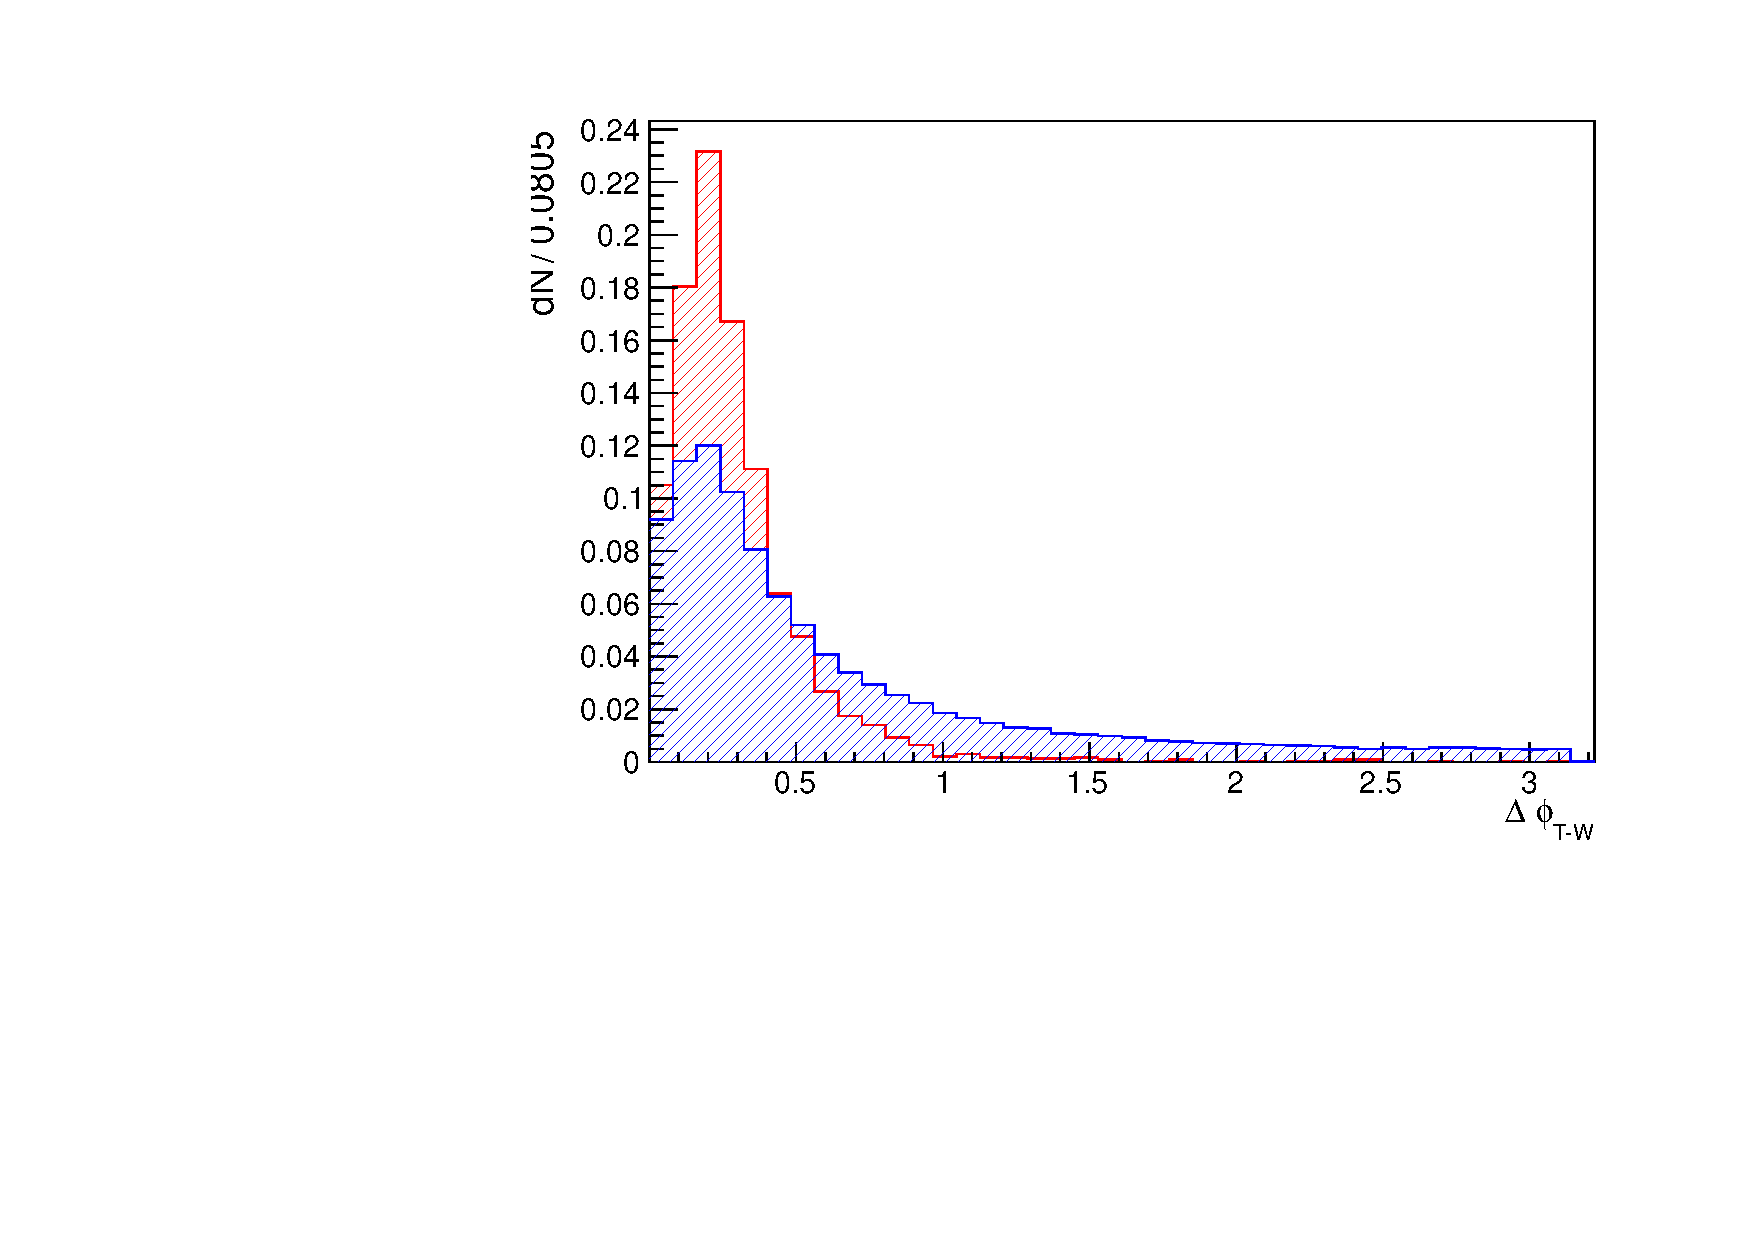
\includegraphics[width=0.49\textwidth]{images/Run1/AnThWh.pdf}
    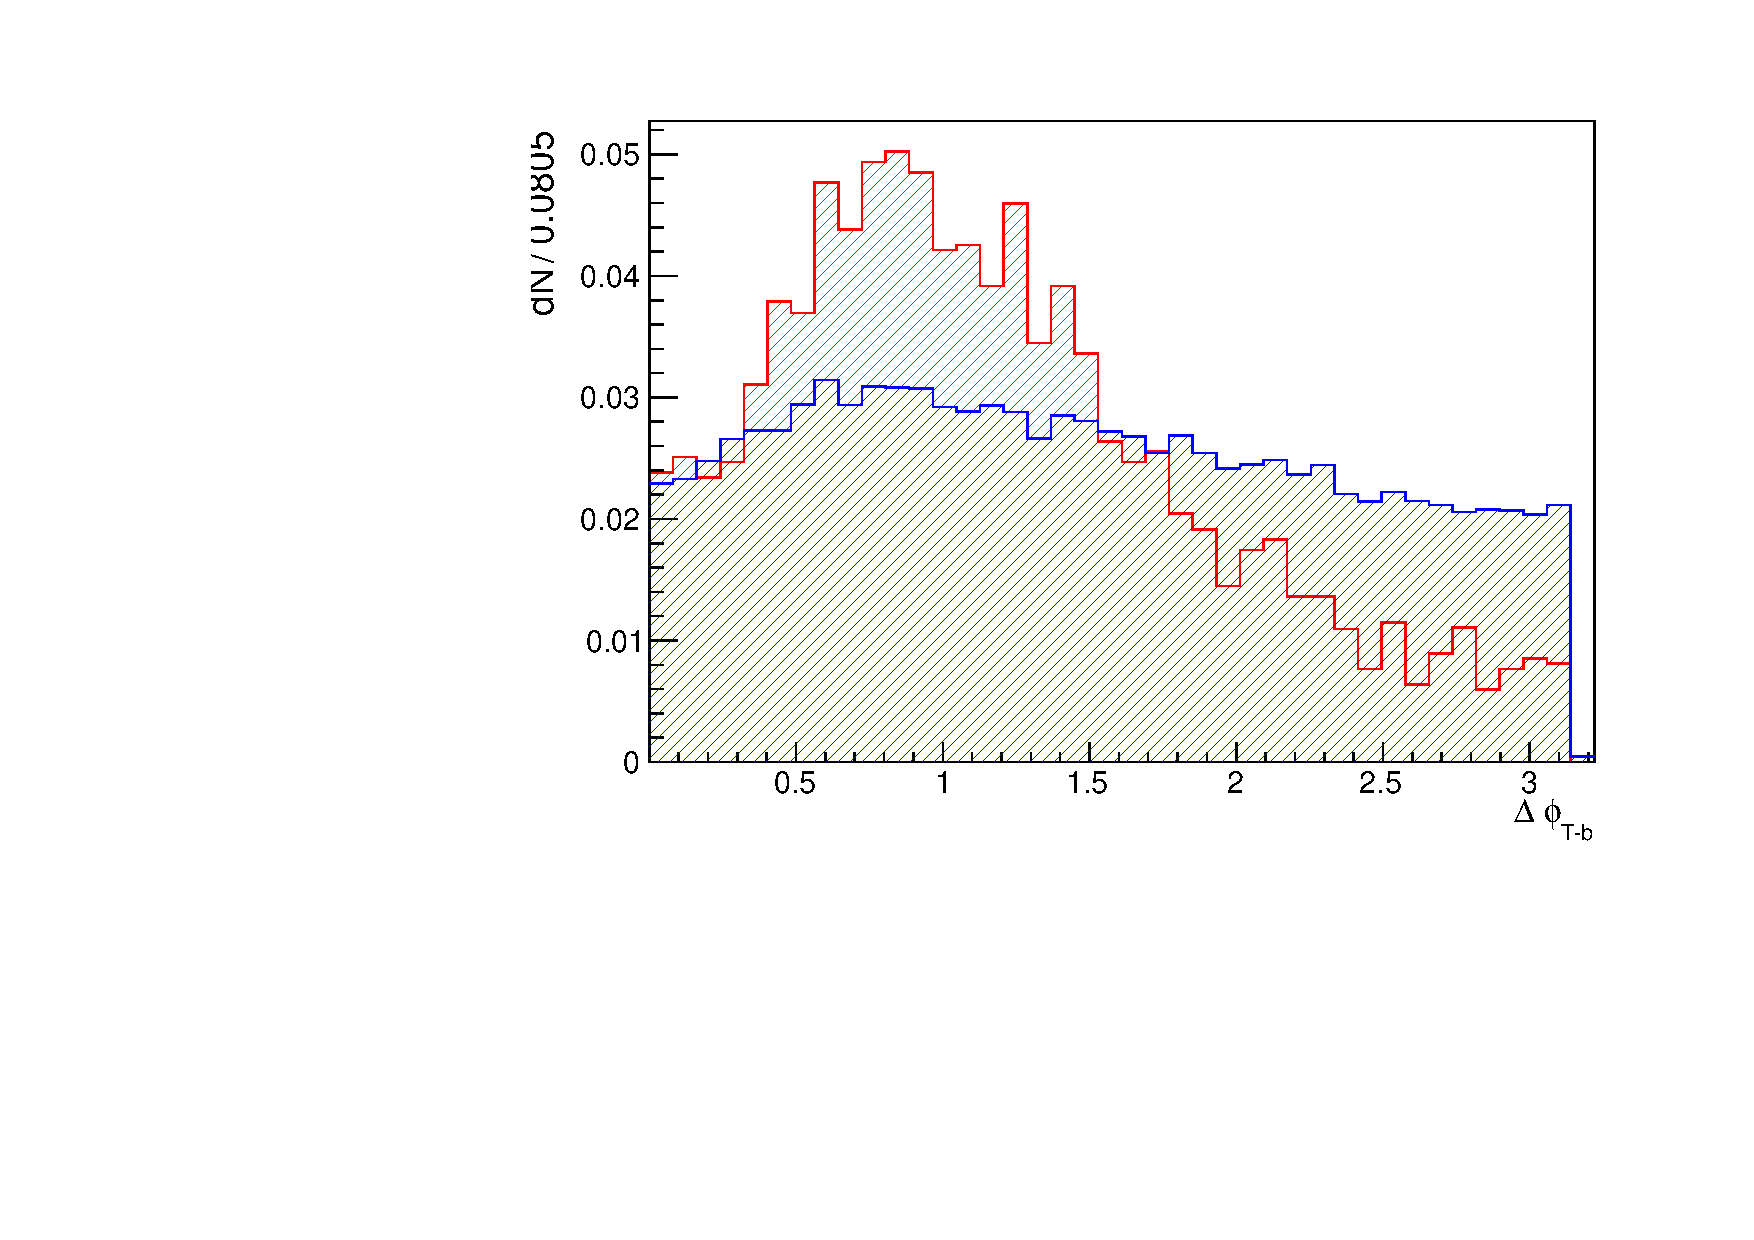
\includegraphics[width=0.49\textwidth]{images/Run1/AnThBh.pdf}
     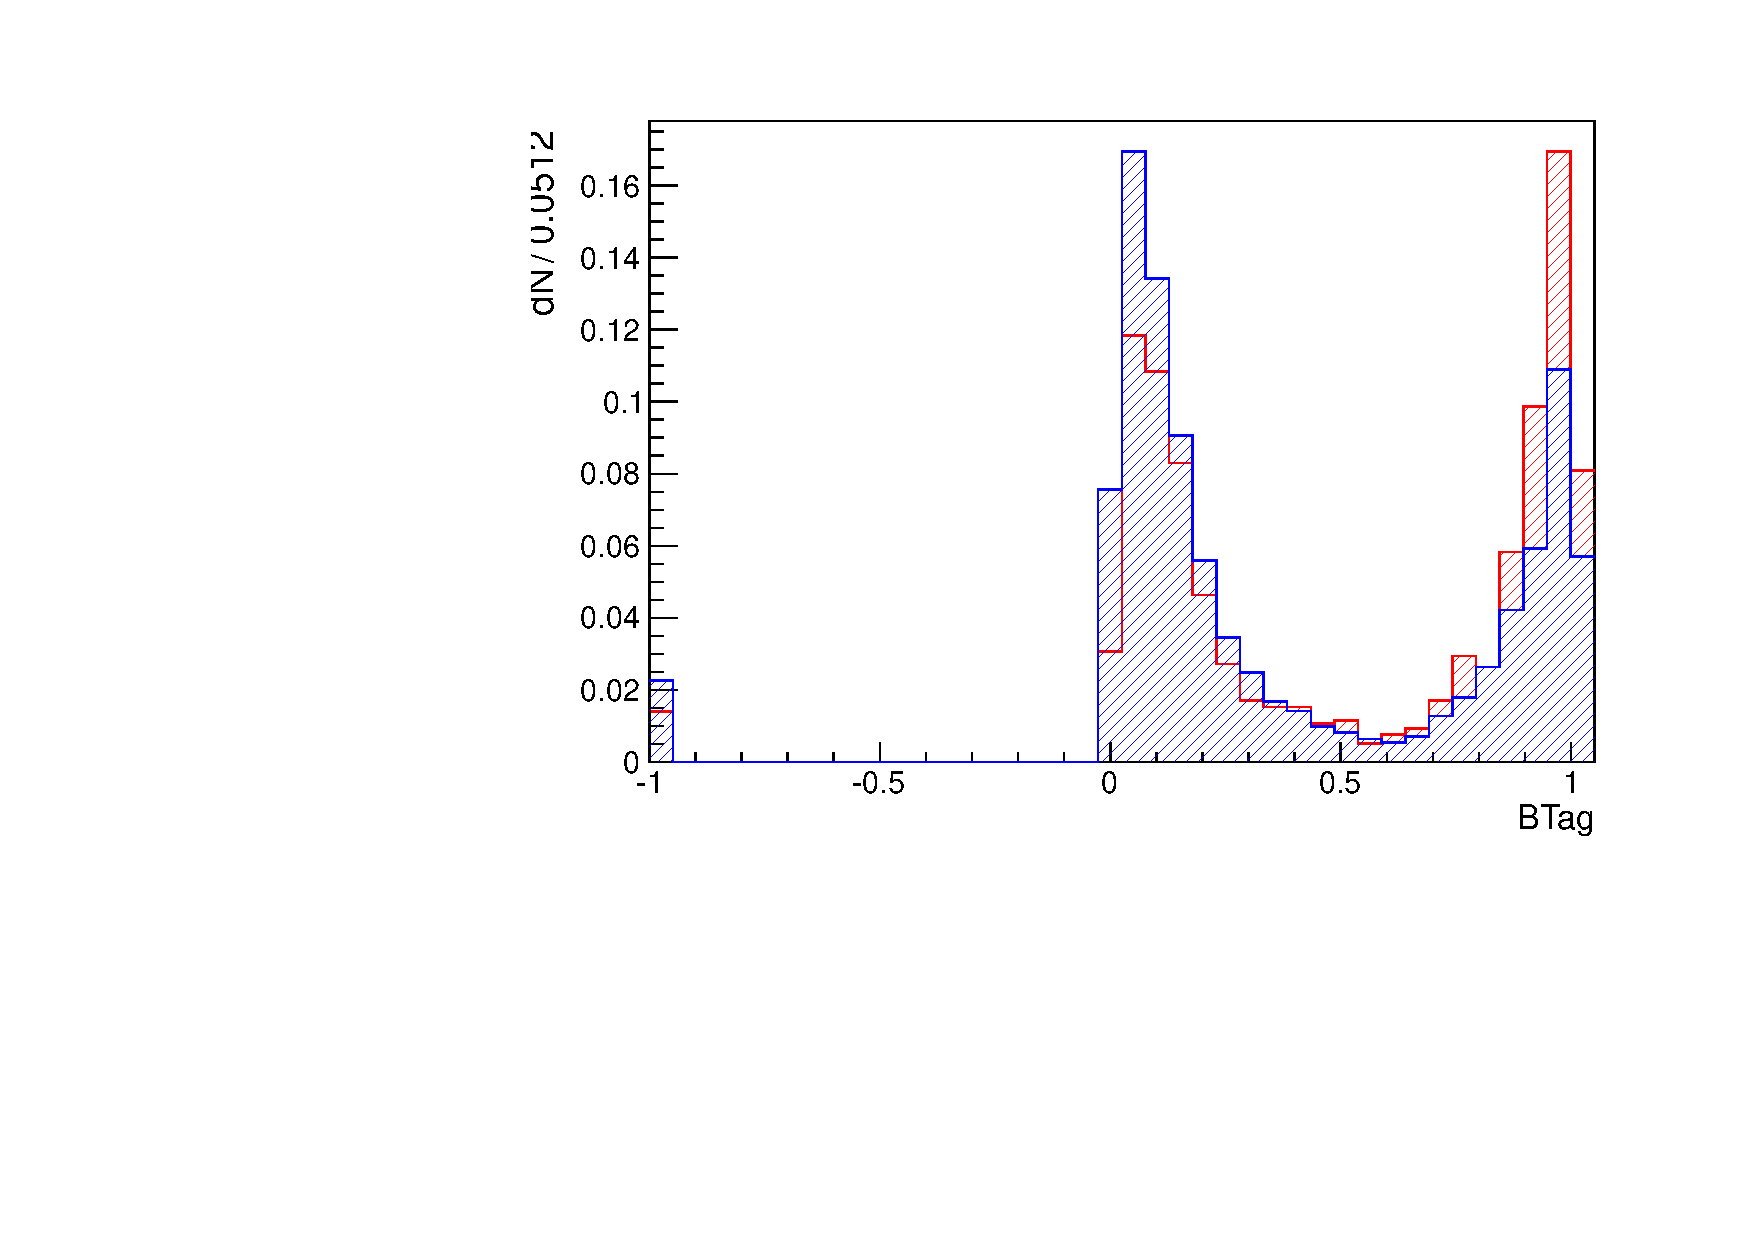
\includegraphics[width=0.49\textwidth]{images/Run1/BTag.pdf}          
    \caption{Input variables into hadronic top quark reconstruction BDT including: the invariant mass of trijets (top-left), the invariant mass of dijets (top-right), the $\pt^{Ratio}$ (middle-left), $\Delta\phi_{T-W}$ between the top quark and dijet (middle-right), $\Delta\phi_{T-b}$ between the top quark and bottom jet (bottom-left) and BTag, which is the CSV value for the jet not in the di-jet (bottom-right).}
    \label{fig:TopBDTinput}
\end{figure}

% The multi-variate analysis tool chosen to calculate a variable to discriminate between good and bad tri-jet combinations is a BDT. The BDT is described in more detail in Section~\ref{sec:BDT}. 
The distribution of the discriminator values output from the BDT is shown in Fig.~\ref{fig:TopBDToutput}, along with a plot of the tri-jet vs BDT value, where the features in the shape are caused by the large discriminating power of the tri-jet and di-jet invariant mass. It can be seen in the tri-jet vs BDT output value plot that tri-jet candidates with an invariant mass close to the top mass are associated with larger BDT output values and, in particular, there is a minimum in the BDT discriminator value at $\approx -0.5$ which can be understood as the division between the two peaks in the BDT discriminator plot. Tri-jets with an invariant mass $\gtrsim 300$~GeV tend to have BDT discriminator values $< -0.5$.

\begin{figure}[!ht]
\centering
    \includegraphics[width=0.49\textwidth]{images/Run1/BDT_Disc.pdf}
    \includegraphics[width=0.49\textwidth]{images/Run1/TrijetmassVsBDT.png}
    \caption{Output discriminator variable from top quark reconstruction BDT (left) and tri-jet mass vs BDT score (right)}
    \label{fig:TopBDToutput}
\end{figure}

\subsubsection*{BDT$_{tri-jet2}$}
% Multitopness is defined to be the BDT discriminator value of the second highest ranking tri-jet after the first highest-ranking tri-jet has been removed from the collection and the remaining jets have been passed through the BDT again. The multitopness value should have values close to 1 for events where there is a second reconstructible top and a value close to -1 where there is only one reconstructible top which has been removed from the collection and the remaining jets are from ISR or FSR. 
The distributions of the BDT$_{tri-jet2}$ variable are shown in Fig.~\ref{fig:Multitopness} for the muon and electron channel. It can be seen that the data and simulation agree well. There is some difference between the shape of the signal and background distributions which can be exploited by the event-level BDT.
%The interesting features in the distributions shape come from the  BDT. 
%The two strongest variables, the tri-jet invariant mass and the di-jet invariant mass, split the dataset sharply into two and then four main sections.

\begin{figure}[!ht]
    \includegraphics[width=0.49\textwidth]{images/Run1/figures/MultiTopness_Mu.pdf}
    \includegraphics[width=0.49\textwidth]{images/Run1/figures/MultiTopness_e.pdf}
    \caption{BDT$_{tri-jet2}$ in data and simulation for $\mu$ + jets (right) and e + jets (left).}
    \label{fig:Multitopness}
\end{figure}

\subsubsection*{Reduced Event Variables}
% New event variables are constructed from removing the highest ranking tri-jet from the jets collection to created a reduced event. These reduced event variables exploit the fact the \ttbar events should only have softer jets remaining from ISR and FSR, whereas \tttt events should have ore energetic jets from the two additional hadronic top quarks.

% \textbf{\HTX} - This is the \HT of the reduced event.\\
% \textbf{\sumjetmassX} - Invariant mass of all jets contained in the reduced event.

Plots for the \HTX and \sumjetmassX reduced variables, which are derived from the reduced event where jets from the highest ranked hadronic top quark candidate are removed, can be seen in Figs~\ref{fig:HTX},~\ref{fig:sumjetmassX}. These variables have excellent agreement between data and simulation and it is apparent, particularly in the \HTX distribution, that these variables will provide some discrimination power in the event-level BDT.

\begin{figure}[!ht]
    \includegraphics[clip, trim=0.15cm 0.15cm 0.15cm 0.1cm, width=0.49\textwidth]{images/Run1/HTX_StackLogY_Mu.pdf}
    \includegraphics[clip, trim=0.15cm 0.15cm 0.15cm 0.1cm, width=0.49\textwidth]{images/Run1/HTX_StackLogY_e.pdf}
    \caption{\HTX for $\mu$ + jets (right) and e + jets (left).}
    \label{fig:HTX}
\end{figure}

\begin{figure}[!ht]
    \includegraphics[clip, trim=0.15cm 0.15cm 0.15cm 0.1cm, width=0.49\textwidth]{images/Run1/SumJetMassX_StackLogY_Mu.pdf}
    \includegraphics[clip, trim=0.15cm 0.15cm 0.15cm 0.1cm, width=0.49\textwidth]{images/Run1/SumJetMassX_StackLogY_e.pdf}
    \caption{\sumjetmassX for $\mu$ + jets (right) and e + jets (left).}
    \label{fig:sumjetmassX}
\end{figure}

% \subsection{b-jet content}
% \label{sec:bottomContent}
% Top quarks decay almost exclusively into bottom quarks by \cPqt $\rightarrow$ \cPqb \Wplus or \cPaqt $\rightarrow$ \cPaqb \Wminus. Therefore, it should be possible to use the number of bottom quarks in the event to distinguish between \tttt events, which should have four bottom quarks in comparison to \ttbar + jets events which typically have two bottom quarks. However this variable does not help to distinguish between \tttt and \ttbb as \ttbb will also have four bottom quarks in the final state. Also \ttbar + jets may have additional bottom quarks arising from the ISR or FSR. 


\subsection{Event activity and b-jet content variables chosen for the event-level BDT}
\label{sec:eventActivity}
% Many variables can be derived by utilising the fact that \tttt events can have up to 10 hard jets whereas \ttbar events should only have up to 4 hard jets. This difference in hadronic activity is exploited by forming the following variables:\\
% \textbf{\njets} - The number of jets is an obvious variable for distinguishing between \tttt and \ttbar. It can be seen in Fig.~\ref{fig:datasimnjets}. \\
% \textbf{\HTb} - The scalar sum of the \pt of the b-tagged jets in the event. Bottom quarks which come from top quark decays tend to have higher \pt than bottom quarks which come from gluon splitting and other processes. As \tttt events should contain four b-quarks which come from top decays and \ttbar events contain two b-quarks from top decays, this variable should be larger for \tttt events, as can be seen in Fig.~\ref{fig:HTb}.\\
% \textbf{Centrality} - This is defined as the ratio of the \HT in the event to the H in the event, where H is the scalar sum of the total momentum (P) in the event.\\
% \textbf{\HTrat} - This is defined as the ratio of the \HT of the four leading jets to the \HT of the other jets in the event. For \ttbar, which should have only four hard jets, this ratio should be larger than \tttt which should have a value closer to one as the four hardest jets are balanced be additional hard jets in the event. \\
% \textbf{5th jet \pt} - After the four leading hard jets in \ttbar, the 5th jet should have, on average, a lower momentum in \ttbar events than in \tttt events. This can be seen in Fig.~\ref{fig:5thjetpt}.\\
% \textbf{6th jet \pt} - Again, the \pt of the 6th jet in \ttbar events should be, on average, lower than in \tttt where the 6th jet is still coming from a hard process. This can be seen in Fig.~\ref{fig:6thjetpt}.\\

The variables chosen for use in the event-level BDT due to their discrimination power include:
\begin{multicols}{2}
\begin{itemize}
\item \njets
\item \nMtags
\item \HTb
\item Centrality
\item \HTrat
\item 5th jet \pt
\item 6th jet \pt
\item BDT$_{tri-jet2}$
\item \sumjetmassX
\item \HTX
\end{itemize}
\end{multicols}
These variables are fully described in section~\ref{sec:MVAtechniques}. All of the variables in Figures~\ref{fig:HTb}-~\ref{fig:6thjetpt} show good agreement between data and simulation and the discriminating power is quite apparent in the distributions of Centrality and \HTrat in Fig.~\ref{fig:centrality} and Fig.~\ref{fig:HTrat}, respectively. Fig~\ref{fig:datasimnbtags} shows the distribution of \nMtags which again shows good agreement between data and simulation and it can be seen that the \tttt signal is more likely to produce events with a higher number of \nMtags than the background due to having four b-quarks in the final state.


\begin{figure}[!ht]
    \includegraphics[clip, trim=0.15cm 0.15cm 0.15cm 0.1cm, width=0.49\textwidth]{images/Run1/HTb_SelectedJets_StackLogY_Mu.pdf}
    \includegraphics[clip, trim=0.15cm 0.15cm 0.15cm 0.1cm, width=0.49\textwidth]{images/Run1/HTb_SelectedJets_StackLogY_e.pdf}
    \caption{\HTb for $\mu$ + jets (right) and e + jets (left).}
    \label{fig:HTb}
\end{figure}

\begin{figure}[!ht]
    \includegraphics[clip, trim=0.15cm 0.15cm 0.15cm 0.1cm, width=0.49\textwidth]{images/Run1/HTH_StackLogY_Mu.pdf}
    \includegraphics[clip, trim=0.15cm 0.15cm 0.15cm 0.1cm, width=0.49\textwidth]{images/Run1/HTH_StackLogY_e.pdf}
    \caption{Centrality for $\mu$ + jets (right) and e + jets (left).}
    \label{fig:centrality}
\end{figure}

\begin{figure}[!ht]
    \includegraphics[clip, trim=0.15cm 0.15cm 0.15cm 0.1cm, width=0.49\textwidth]{images/Run1/HTRat_StackLogY_Mu.pdf}
    \includegraphics[clip, trim=0.15cm 0.15cm 0.15cm 0.1cm, width=0.49\textwidth]{images/Run1/HTRat_StackLogY_e.pdf}
    \caption{\HTrat for $\mu$ + jets (right) and e + jets (left).}
    \label{fig:HTrat}
\end{figure}

\begin{figure}[!ht]
    \includegraphics[clip, trim=0.15cm 0.15cm 0.15cm 0.1cm, width=0.49\textwidth]{images/Run1/5thJetPt_StackLogY_Mu.pdf}
    \includegraphics[clip, trim=0.15cm 0.15cm 0.15cm 0.1cm, width=0.49\textwidth]{images/Run1/5thJetPt_StackLogY_e.pdf}
    \caption{5th jet \pt for $\mu$ + jets (right) and e + jets (left).}
    \label{fig:5thjetpt}
\end{figure}

\begin{figure}[!ht]
    \includegraphics[clip, trim=0.15cm 0.15cm 0.15cm 0.1cm, width=0.49\textwidth]{images/Run1/6thJetPt_StackLogY_Mu.pdf}
    \includegraphics[clip, trim=0.15cm 0.15cm 0.15cm 0.1cm, width=0.49\textwidth]{images/Run1/6thJetPt_StackLogY_e.pdf}
    \caption{6th jet \pt for $\mu$ + jets (right) and e + jets (left).}
    \label{fig:6thjetpt}
\end{figure}

\subsection{Event-level BDT}
% All of the variables described in Sections~\ref{sec:topContent},~\ref{sec:bottomContent} \&~\ref{sec:eventActivity} are used in a BDT, known as the event-level BDT. It is necessary to use 
A sample of events which were not used to train the kinematic reconstruction of top quarks are used to train the event-level BDT so that an orthogonal training sample can be provided. 
% An additional set of events are used to test the performance of the BDT. 
The output distribution of the BDT discriminator can be seen in Fig.~\ref{fig:BDT}. Again, there is good agreement between the data and simulation and it can be seen that there is an improved separation between the background distributions and the \tttt distribution compared to the input variables to the BDT.
% \fxnote{Numbers of events for training?}

\begin{figure}[!ht]
    \includegraphics[width=0.49\textwidth]{images/Run1/figures/MVA_Mu.pdf}
    \includegraphics[width=0.49\textwidth]{images/Run1/figures/MVA_e.pdf}
    \caption{BDT discriminator variable in data and simulation for $\mu$ + jets (right) and e + jets (left).}
    \label{fig:BDT}
\end{figure}

\section{Systematic uncertainties}
\label{sec:uncertainties8}
% There are two categories of systematic uncertainties; (i) Uncertainties which affect the normalisation of the distributions which are applied to signal and background and (ii) uncertainties which affect the shape of the distributions which are applied to the dominant background, in this case \ttbar. 

All systematic uncertainties are described in section~\ref{sec:uncertainties} and some further details about them are given below.

% \subsection{Normalisation uncertainties}
% %The normalisation uncertainties will only affect the uncertainty on the expected limit rather than the limit itself when it is used in the template fit and limit setting procedure described in Section~\ref{sec:limit}.
% Normalisation uncertainties include the following:
\begin{itemize}
\item \textbf{Luminosity}\\
The CMS Luminosity Group gave a recommendation of 2.6$\%$ uncertainty on the luminosity~\cite{CMS-PAS-LUM-12-001}.
\item \textbf{Monte Carlo cross sections}\\
As \ttbar is the main background to \tttt, the uncertainty on its MC cross-section is expected to be one of the dominant systematic uncertainties. The uncertainty on \ttbar is ${}^{+2.5\%}_{-3.4\%} \left( \textrm{renormalisation and factorisation scale} \right)$ and ${}^{+2.5\%}_{-2.6\%} \left( \textrm{PDF} \right)$~\cite{PhysRevLett.110.252004}. The MC cross section uncertainties for the other background processes are modelled by assigning a $4\%$ uncertainty and a $10\%$ uncertainty is assigned to the signal process.
\item \textbf{Factorisation and renormalisation scales}\\
The alternative \ttbar samples with ME and PS scale (u) varied by 2u, 1/2u were used as the alternative shapes.
\item \textbf{Matching threshold}\\
The alternative \ttbar samples with the matching threshold changed between 20~GeV and 40~GeV were used as the alternative shapes.
\item \textbf{JES}\\
The JES uncertainty is derived by varying the JES by $\pm1\sigma$.
\item \textbf{JER}\\
The JER uncertainty is derived by varying the smearing by $\pm1\sigma$.
\item \textbf{b tagging}\\
The b tagging uncertainty is quantified by varying the scale factor by $\pm1\sigma$.
\item \textbf{Pile up}\\
The PU systematic uncertainty is found by varying the MinBias cross section by $\pm5\%$.
\item \textbf{\heavyflavourone / \heavyflavourtwo modelling}
The uncertainty on the measurement of \heavyflavourone / \heavyflavourtwo by CMS~\cite{Khachatryan2015132} is $\pm 0.4 \left( \textrm{stat.} \right) \pm 0.5 \left(\textrm{sys.} \right)$. Alternative event weights are derived for \heavyflavourone / \heavyflavourtwo which are used to provide the alternative systematic up and down templates.
 \end{itemize}
 \fxnote{mistag?}
 
% The analysis procedure is repeated with \ttbar samples which have the respective quantity varied by $\pm 1 \sigma$ in order the produce new BDT templates with a deviated shape However, in the case of the matching threshold, the alternative shapes are produced by varying the matching threshold up to 40 GeV and down to 20 GeV.

\section{Template fit and upper limit}
\label{sec:limit}

An upper limit was calculated on the signal strength, $\sigmatttt~/~\sigmattttSM$. No excess was observed in the data. Firstly, a template fit of the BDT distributions is made using the Combine Tool~\cite{CMS-NOTE-2011-005} which is based on he statistal package RooStats~\cite{RooStats:2010,Read:2002hq,Junk:1999kv,Cowan:2011js}.
% , where the systematic uncertainties are modelled as nuisance parameters. Shape uncertainties are constrained using gaussian terms with exponential interpolation whereas the normalisation uncertainties are constrained using lognormal terms. For the statistical uncertainties, a lightweight version of the {Beeston and Barlow method~\cite{Conway:2011in} was used. This gives one nuisance parameter for the total MC estimate and a statistical uncertainty on each bin. 
The background processes are grouped into the following templates for the fit: `\ttbar' for semi-leptonic \ttbar, `electroweak' for W $+$ jets and Z $+$ jets, and `\ttbar\textunderscore other' for all other \ttbar processes. Using the \CLS method~\cite{Junk1999435,0954-3899-28-10-313} with the asymptotic approximation, the best fit values of the nuisance parameters can be obtained along with the corresponding limit on $\sigmatttt~/~\sigmattttSM$. The cross section limit, \sigmatttt, can be derived by multiplying $\sigmatttt~/~\sigmattttSM$ by \sigmattttSM $1.3$.

\subsection{Splitting into \njets categories}
\label{sec:njetcatlimit}
To increase the sensitivity of the analysis, the BDT templates were split into three \njets categories (\njets $= 6$, \njets $= 7 $ \& \njets $\geq 8$) for each of the muon and electron channels. The higher \njets categories benefit from better discrimination power between signal and background as \tttt events are likely to have a larger number of jets. The \njets $= 6$ category helps to constrain the main background of \ttbar. A simultaneous fit of these three \njets categories is made for the muon channel, the electron channel and a combination of the two. The limits extracted using the \CLS method are shown in Table~\ref{tab:lims}.


\begin{table}[ht!]
\centering
\begin{tabular}{| l | l | l | p{1cm} |}
 \hline 
 Channel & Exp.  &Obs. \\
   \hline
 $\mu$ + jets & $35.6\pm 18$ & 34 \\
  \hline
$e$ + jets &  $36.1\pm16$  & 36  \\
\hline
 combined & $24.6\pm13$  & 25   \\
\hline
\end{tabular}
\hspace{0.5cm}
\begin{tabular}{| l | l | l | p{1cm} |}
 \hline 
 Channel & Exp. (fb) &Obs. (fb) \\
   \hline
 $\mu$ + jets & $46.3\pm23$ & 44 \\
  \hline
$e$ + jets &  $47.0\pm20$  & 47  \\
\hline
 combined & $32.0\pm17$  & 32   \\
\hline
\end{tabular}
\caption{CLS limits on (\sigmatttt/(\sigmattttSM) (left) and \sigmatttt (right). }
\label{tab:lims}
\end{table}

In comparison, the corresponding limit for a simultaneous fit of the electron and muon channels in an inclusive \njets category was observed to be 63~fb with an expected limit of  $42^{+18}_{-13}$~fb~\cite{CMS-PAS-TOP-13-012}. Therefore, it can be seen that splitting into \njets categories provides a significant improvement in the sensitivity of the analysis.

\section{Systematics studies and tests on analysis\label{studies8}}

\subsection{Signal Injection Test}
\label{sec:signalinjection}
In order to validate the limit-setting method, the following closure test was performed. A range of signal strengths were injected into the data to simulate what the data collected by CMS would be with an enhanced \tttt cross section and the limit-setting procedure was repeated. Figure~\ref{fig:SigInjection} shows the BDT discriminator distributions with injected signal strengths of 20fb, 40fb and 60fb. With the increasing signal strength, there is an increase for data in the bins with a higher BDT discriminator values as would be expected for signal events.

\begin{figure}[ht!]
\centering
    \includegraphics[width=0.49\textwidth]{images/Run1/SignalInjection_Mu_6j.pdf}
     \includegraphics[width=0.49\textwidth]{images/Run1/SignalInjection_El_6j.pdf}
    \includegraphics[width=0.49\textwidth]{images/Run1/SignalInjection_Mu_7j.pdf}
     \includegraphics[width=0.49\textwidth]{images/Run1/SignalInjection_El_7j.pdf}
    \includegraphics[width=0.49\textwidth]{images/Run1/SignalInjection_Mu_8j.pdf}
     \includegraphics[width=0.49\textwidth]{images/Run1/SignalInjection_El_8j.pdf}          
    \caption{The BDT discriminator distributions of data and the mixtures of data and injected signal are compared for $\mu$ + jets channel $\left( \textrm{left} \right)$ and e + jets channel $\left( \textrm{right} \right)$. }
    \label{fig:SigInjection}
\end{figure}

\begin{figure}[!ht]
\centering
    \includegraphics[width=0.6\textwidth]{images/Run1/SignalInjection_JS_Brazil.pdf}
    \caption{Fitted values(fb) and observed(fb) for various injected signal strength(fb).}
    \label{fig:SigInjectionBrazil}
\end{figure}

As can be seen in Fig.~\ref{fig:SigInjectionBrazil}, the fitted value for the signal strength and observed limit increase with increasing injected singal strength as expected. This shows that the analysis is capable of detecting an enhanced signal if it were present. However, there appears to be some bias in the analysis towards selecting background as opposed to signal as can be seen from the gradient of the line, which is $<$1.

% \subsection{Systematics studies}

\subsection{Negligible uncertainties}
\emph{This study was undertaken before the decision was made the split the BDT templates by the \njets categories.}

Additional systematic uncertainties were studied which ultimately had a negligible impact on the analysis so were not included in the final result. For completeness they are discussed here.

In the 2012 CMS differential cross-section \ttbar analysis \cite{CMS:TopPt} the \pt spectrum of top quarks tends towards higher values in the \MADGRAPH simulation than it is in data. Scale factors were derived by CMS to compensate for this effect. The analysis was performed with and without the application of the top \pt scale factors and the observed effect was negligible, as seen in Fig.~\ref{fig:studies8}, and hence these scale factors were not applied for the final result and no systematic uncertainty was included.\\
The uncertainty on the parton distribution functions (PDFs) are a potential source of systematic uncertainty. The method used by CMS to model this effect is given in~\cite{ref:PDFUnc2}. The BDT distributions which correspond to the maximal downward and upward fluctuation due to the uncertainty on the PDFs have a very small effect on the shape of the BDT, as seen in Fig.~\ref{fig:studies8}, and are not considered further.\\
The uncertainty due to the choice of \PYTHIA tune used in the hadronisation of \ttbar events is considered. The nominal tune used is the $Z2^{*}$ tune which is compared to the alternative $P11$ tune. Again, there is a very small effect on the shape of the BDT, as seen in Fig.~\ref{fig:studies8}, so this uncertainty is not included in the final fit.

\begin{figure}[ht!]
\centering
    \includegraphics[width=0.49\textwidth]{images/Run1/ptrw_xcheck.pdf}
    \includegraphics[width=0.49\textwidth]{images/Run1/NomTune_Mu_Log.pdf}\\
        \includegraphics[width=0.7\textwidth]{images/Run1/PDF_uncertainty_mu.pdf}
    \caption{The BDT discriminator distributions of \ttbar simulation with and without the top quark \pt reweighting (top left), \PYTHIA tunes (top right) and PDF uncertainty (bottom)}
    \label{fig:studies8}
\end{figure}


\subsection{Individual effects of systematics}

To deduce how much of an effect each shape systematic has on the results, the expected limits were recalculated multiple times with one of the systematic effect removed. These limits are denoted lim.$_{1}$. In addition, another set of limits are calculated with only one of the systematic uncertainties included. These limits are denoted lim.$_{1}$. The values of lim.$_{1}$ and lim.$_{2}$ for each systematic uncertainty are detailed in Table~\ref{tab:effectLims}.

\begin{table}[ht!]
\small
\centering
\begin{tabular}{|c |c |c | c | c | c |}
\hline
 Sys. &  exp. lim.$_{1}$ & exp. lim.$_{2}$   \\
 \hline  
None & $32.0^{+17}_{-17}$ & $32.0^{+17}_{-17}$ \\
 \hline 
 JER &    $33.15^{+13.84}_{-10.35}$  &  $30.19^{+14.21}_{-9.66}$    \\
 \hline  
 JES  & $31.62^{+15.05}_{-9.16}$ &  $23.31^{+12.25}_{-8.05}$     \\
\hline  
Matching &  $32.79^{+14.37}_{-10.21}$ & $32.79^{+14.37}_{-10.21}$     \\  
 \hline  
 PU    &  $32.42^{+13.91}_{-10.00}$  &  $28.05^{+13.32}_{-8.93}$    \\
 \hline  
 Scale  &  $32.46^{+14.56}_{-10.35}$ & $24.80^{+13.21}_{-6.73}$       \\
 \hline  
 bTag &  $33.40^{+14.27}_{-10.48}$ & $23.32^{+12.71}_{-8.35}$       \\
 \hline  
 leptonSF &  $33.36^{+14.24}_{-10.39}$  &  $28.20^{+13.32}_{-8.96}$   \\  
 \hline  
 misTag &  $33.24^{+14.14}_{-10.34}$  &  $28.62^{+13.46}_{-9.13}$  \\
 \hline  
 ttbb  &  $33.23^{+13.87}_{-10.17}$  &  $27.97^{+13.26}_{-8.91}$  \\
 \hline
\end{tabular}
\caption{Effects of systematic uncertainties. }
\label{tab:effectLims}
\end{table}

\subsection{Cross checks with Theta package and the fully-frequentist approach using Combine}

A cross-check was performed using the Theta package~\cite{theta} to set a limit using \CLS with the asymptotic approximation. As another cross-check, the fully frequentist \CLS limit setting procedure is performed, using Combine, in place of the asymptotic limit setting used for the final results. Due to the extremely large CPU demands of the fully frequentist technique the range of values for the parameter of interest, $\frac{\sigma_{tttt}}{\sigma_{tttt}^{SM}}$, and the number of points investigated is reduced. The results, shown in Table~\ref{tab:ThetaFreq}, are consistent with the results obtained using the asymptotic approximation in Combine.


\begin{table}[ht!]
\centering
\begin{tabular}{|l|r|r|r|r|}
 \hline 
 Setup & Exp.$\frac{\sigma_{signal}}{\sigma_{SM}^{t\bar{t}t\bar{t}}}$ & Obs.$\frac{\sigma_{signal}}{\sigma_{SM}^{t\bar{t}t\bar{t}}}$ & Exp.(fb) &Obs.(fb) \\ 
\hline
{\color{blue}Combine (asymptotic.)} & {\color{blue} 24.6 $\pm$ 13}  & {\color{blue}24.7} & {\color{blue} 32  $\pm$ 17}  & {\color{blue}32} \\
\hline
%Theta (asymptotic) & 21.9^{+10}_{-6} & 22.33 & 28.47^{+13}_{-8} & 29.02 \\
Theta (asymptotic) & $27.4^{+12}_{-8}$ & 24.66 & $35.6^{+16}_{-10}$ & 32 \\
 \hline
%Combine (ful. freq.) &  -  & 20.52 &  -  & 26.68 \\
Combine (ful. freq.) &  -  & 23.78 &  -  & 31 \\
\hline
\end{tabular}
\caption{CL$_S$ limits on $\sigma_{t\bar{t}t\bar{t}}$ from combine (asymptotic + fully frequentist) and Theta approaches.}
\label{tab:ThetaFreq}
\end{table}


\subsection{Fitted nuisance parameters and uncertainties}

% As previously described in Section~\ref{sec:limitsJS}, the four largest shape uncertainties (Scale, Matching, JES and B-tag scale factor) are constrained in the fit using gaussian terms with exponential interpolation. The nuisance parameters associated to the other shape systematics are constrained in the fit using gaussian terms and the nuisance parameters associated to the normalisation uncertainties are constrained in the fit using lognormal terms. 

In Table~\ref{tab:nuisBSB} the fitted values, $\Delta x$, and the post-fit uncertainties, $\sigma_{\text{out}}$, in units of the input uncertainty, $\sigma_{\text{in}}$, are given for the background only (b-only) hypothesis and the signal + background (s+b) hypothesis. If the associated uncertainty is well modelled, the value of $\frac{\Delta x}{\sigma_{\text{in}}}$ should be close to zero and the value of $\frac{\sigma_{\text{out}}}{\sigma_{\text{in}}}$ should be close to one. The largest deviations in $\frac{\sigma_{\text{out}}}{\sigma_{\text{in}}}$ arise from the scale and matching uncertainties, which is expected as these uncertainties were assigned ad hoc variations. Table~\ref{tab:nuisBSB} shows that the results do not vary significantly between the b-only and s+b hypothesises which is consistent with no signal being present in the data.

\begin{table}[ht!]
\centering
\begin{tabular}{|l|r|r|r|r|} \hline 
&  \multicolumn{2}{c|}{$b$-only fit } & \multicolumn{2}{c|}{$s+b$ fit} \\ 
name  &  $\Delta x/\sigma_{\text{in}}$ & $\sigma_{\text{out}}/\sigma_{\text{in}}$ & $\Delta x/\sigma_{\text{in}}$ &$\sigma_{\text{out}}/\sigma_{\text{in}}$  \\  \hline
btag                        &   +0.16 &  1.15 &   +0.16 & 1.24  \\
ew\_norm               &    -0.01 &  0.99 &   -0.00  & 0.99  \\
JER                           &    +0.64 &  0.48 &  +0.63 & 0.49  \\
JES                          &    +0.30 &  0.37 &  +0.29  & 0.37  \\
lepton sf                  &    -0.02  &  1.19 &  -0.02  & 1.29  \\
lumi                        &    -0.92  &  0.81 &  -0.93  & 0.82  \\
matching                &    -0.30  &  0.17 &   -0.30 & 0.17  \\
mistag                    &    +0.22  & 1.04 &  +0.27 & 1.05  \\
pu                           &    +0.27 &  0.82 &  +0.28 & 0.86  \\
scale                      &     +0.12 &  0.25 &  +0.11 & 0.27  \\
tt\_norm                 &     -1.34  &  0.61 &  -1.35  & 0.62 \\
ttbb                        &      +0.18 &  0.84 & +0.20 & 0.87  \\
ttother\_norm         &     -0.06   & 0.99 &  -0.06 & 0.99  \\
\hline
\end{tabular}
\caption{Fitted values and post-fit uncertainties in units of input uncertainties ($\sigma_{in}$) for nuisance parameters in $b$-only and $s+b$ fits.}
\label{tab:nuisBSB}
\end{table}

% \subsection{Goodness-of-fit test}

% A goodness-of-fit test for a maximum likelihood fit based on a saturated model \cite{ref:CousinsSat} is also performed. A likelihood ratio ($\lambda$) is calculated in which the numerator is the value of the maximised likelihood function in the fit and the denominator is the maximum value of a likelihood function of a \emph{saturated model} i.e., a model that fits the data exactly. The quantity $-2 ln(\lambda)$ asymptotically follows a $\chi^{2}$ distribution and hence can be used as a test of the goodness of fit. Distributions are shown  for the background only hypothesis and the signal+background hypothesis in Fig. \ref{fig:GOF}. The corresponding p-value obtained for the fit using the method just described are provided below and indicate a good fit.

% \begin{centering}
% \begin{equation*}
% \centering
% p-value^{b-only} = 0.65 , \;\;\;\; p-value^{s+b} = 0.64 
% \end{equation*}
% \end{centering}

% \begin{figure}[ht!]
% \centering
%     \includegraphics[width=0.49\textwidth]{goodnessoffit_bonly.pdf}
%      \includegraphics[width=0.49\textwidth]{goodnessoffit_floatingsignal.pdf}
%     \caption{$\lambda$ test-statistic distributions in the b-only(left) and s+b hypotheses(right). }
%     \label{fig:GOF}
% \end{figure}

% \clearpage

\subsection{Alternative parameterisations}

%\subsection{Scale uncertainty}
As the combined ME and PS scale systematic may vary in shape across the \njets categories, another cross-check on the analysis was to allow the scale systematic to vary independently in each \njets category, as in ~\cite{ref:heavyquarksSplit, ref:B2G-12-004}. In this approach, both channels have three nuisance parameters for the scale systematic compared with one nuisance parameter used for all \njets categories. The results, shown in Table~\ref{tab:limsScale}, show no significant change in the limit compared with the original approach. The associated nuisance parameters and their uncertainties are show in Table~\ref{tab:ScaleParamUnc}.

\begin{table}[ht!]
\centering
\begin{tabular}{| l | l | l | p{1cm} |}
 \hline 
$N_{scale \; params.}$ & Exp. (fb) &Obs. (fb) \\
\hline
%1 & 26.3\pm{13}$ & 27 \\
1&{\color{blue} 32  $\pm$ 17}  & {\color{blue}32}\\
 \hline
3  &  $31.8\pm{12}$ & 32.5 \\
\hline
\end{tabular}
\caption{CLS limits on $\sigma_{t\bar{t}t\bar{t}}$ for the nominal result (top row) and with scale uncertainty fit independently in each \njets bin (bottom row). }
\label{tab:limsScale}
\end{table}

\begin{table}[ht!]
\centering
\small
\begin{tabular}{|l|r|r|r|r|} \hline 
 &  \multicolumn{2}{c|}{$b$-only fit } & \multicolumn{2}{c|}{$s+b$ fit} \\
name        &  $\Delta x/\sigma_{\text{in}}$ & $\sigma_{\text{out}}/\sigma_{\text{in}}$ & $\Delta x/\sigma_{\text{in}}$ &$\sigma_{\text{out}}/\sigma_{\text{in}}$  \\  \hline
btag          &    +0.04& 1.35 & -0.04& 1.51 \\
jer             &      +0.43& 0.53 &     +0.42& 0.54 \\
jes            &   +0.30& 0.37 &  +0.28& 0.39  \\
leptonsf    &      -0.01& 1.36 &  -0.02& 1.56 \\
lumi          &      -0.92& 0.81 &     -0.94& 0.82  \\
matching  &   -0.27& 0.19 &  -0.26& 0.19  \\
mistag      &      +0.18& 1.17 &     +0.27& 1.13  \\
pu            &      +0.29& 0.87 &     +0.28& 0.95  \\
scale6j     &   +0.31& 0.23 &  +0.31& 0.23  \\
scale7j     &   +0.31& 0.25 &  +0.31& 0.25  \\
scale8j     &   -0.71& 0.34 &  -0.70& 0.36  \\
tt\_norm   &      -1.33& 0.61 &     -1.36& 0.62  \\
ttbb          &      +0.40& 0.71 &     +0.44& 0.75  \\
 \hline
\end{tabular}
\vspace{-0.2cm}
\caption{Fitted values and post-fit uncertainties in units of input uncertainties ($\sigma_{in}$) for all nuisance parameters in $b$-only and $s+b$ fits.}
\label{tab:ScaleParamUnc}
\end{table}

A separate check was made where the normalisation uncertainty on the $\ttbar$ component was allowed to vary independently in each  \njets category. In each channel, three nuisance parameters are associated to the normalisation uncertainty on the $\ttbar$ for each \njets category compared to the one nuisance parameter across all \njets categories in the original approach. The results, shown in Table~\ref{tab:limsTTnorm}, also show no significant change to the original limit.

%\subsection{t\bar{t}$ normalisation uncertainty}

\begin{table}[ht!]

\centering
\begin{tabular}{| l | l | l | p{1cm} |}
 \hline 
& Exp. (fb) &Obs. (fb) \\
\hline
%1 & 26.3\pm{13}$ & 27 \\
nominal&{\color{blue} 32  $\pm$ 17}  & {\color{blue}32}\\
 \hline
varying tt in \njets bins  &  36 $\pm {17}$ & 41 \\
\hline
\end{tabular}
\caption{CLS limits on $\sigma_{t\bar{t}t\bar{t}}$ for the nominal result (top row) and with tt normalisation uncertainty fit independently in each \njets bin (bottom row). }
\label{tab:limsTTnorm}
\end{table}


\subsection{Using \njets$\geq$8jet category only}

The greatest separation of signal and background occurs in the \njets$\geq8$~jet category as $\tttt$ events are typically higher jet multiplicity events than $\ttbar$. In order to ascertain whether the analysis could benefit from a higher jet multiplicity cut, the limit setting procedure is repeated using only the \njets$\geq8$~jet category. The results are shown in Table \ref{tab:lims8}, where it can be seen that the limit is made worse by removing the \njets$=6$ and \njets$=7$ categories. This implies that including the \njets$=6$ category aids in constraining the $\ttbar$ in the fit. The \njets$=7$ category also has some discrimination between signal and background and simultaneously fitting the \njets$=6$, \njets$=7$ and \njets$\geq8$ categories provides a better limit.

\begin{table}[ht!]
\centering
\begin{tabular}{| l | l | l | p{1cm} |}
 \hline 
  & Exp. (fb) &Obs. (fb) \\
\hline
%nominal result & 26.3\pm{13}$ & 27 \\
 {\color{blue} nominal result}&{\color{blue} 32  $\pm$ 17}  & {\color{blue}32}\\
 \hline
8 jet bin only  &  $45 \pm{ 17}$  & 47 \\
\hline
\end{tabular}
\caption{CLS limits on $\sigma_{t\bar{t}t\bar{t}}$ for nominal scenario and 8 jet bin only. }
\label{tab:lims8}
\end{table}

\subsection{Investigation of binning in BDT distributions \label{appsub:binning}}

In order to ascertain what the optimum binning should be within each BDT distribution, a variety a values are plotted in Fig.~\ref{fig:Binning}. Both the inclusive result before splitting the templates into \njets categories and exclusive \njets categories results are shown, where the significant improvement in the limit by the latter method can be seen. The limit does not appear to improve significantly when increasing the number of bins in the BDT distributions so in order to ensure that most bins were well populated, the number of bins was chosen to be ten in the exclusive analysis. This is so that the simulation is not fitted to statistical fluctuations in data.

\begin{figure}[ht!]
\centering
    \includegraphics[width=0.69\textwidth]{images/Run1/BinningPrint.pdf}
    \caption{Fitted values(fb) and observed(fb) for various injected signal strength(fb).}
    \label{fig:Binning}
\end{figure}

\section{Candidate four-top-quark event}

Although we can never know which specific events are produced from the decays of four top quarks we can find candidate events which are more likely to have come from \tttt production. Figure~\ref{fig:fourtopevent} shows an event from data which has 11 jets, three of which are b-tagged. It has a relatively high event-level BDT score and also a high score from the hadronic top quark BDT, where the \emph{Multitopness} variable on the figure equates to BDT$_{tri-jet2}$. Both the hadronic transverse energy from the reduced event, HTX, and from b-quarks, HTb, is large, as expected for \tttt events. 

\begin{figure}[ht!]
\centering
    \includegraphics[width=0.75\textwidth]{images/Run1/EventDisplay4topsDraft}
    \caption{A candidate four-top-quark event from the \runone 2012 CMS dataset.}
    \label{fig:fourtopevent}
\end{figure}
\section{Summary and conclusion}
\label{sec:summary8}
The full 2012 data set of proton-proton collisions at $\sqrt{s}=8$~TeV with 19.7~\fbinv of data was used to set limits on the production of \tttt in the single muon and single electron final states in the absence of a signal. After a baseline selection the dominant background is \ttbar production. The simulation is corrected with scale factors. Two BDTs are used in the analysis, one for reconstructing hadronically decaying top quarks and one event-level BDT to separate the signal and background using discriminators derived from the hadronic top quark reconstruction BDT. Analysis of the systematic uncertainties showed the factorisation and renormalisation scale on the \ttbar background to be the largest uncertainty. A template fit was performed on the event-level BDT discriminator output which was separated into \njets categories. A simultaneous fit of the templates for the single electron and single muon histograms, each split into \njets categories, was performed and a \CLS limit at $95\%$ CL on $\sigmatttt~/~\sigmattttSM$ of 25 observed and $24.6\pm13$ expected was found. This corresponds to 32~\fb observed with $32.0\pm17$~\fb expected.

\section{Discussion of other searches for \tttt production studies at $\sqrt{s} =$~8~TeV}
\label{sec:ATLASresult}
 
The ATLAS collaboration have also published limits on the \tttt cross section in the single lepton + jets channel at $\sqrt{s}=8$~TeV~\cite{Aad:2015kqa}. This search takes a more simple approach by making an initial selection, splitting events into categories and then making a fit to the \HT distributions. The selection is similar to the selection in this chapter: 1 isolated lepton (e or $\mu$), $\geq 5$ jets, $\geq 2$ b-tagged jets, \MET$>$20~GeV and $(\MET+M_{T}^{W})>60$~GeV (where $M_{T}^{W}$ is the transverse mass of the lepton). The electron and muon channels and considered as one analysis. Events are categorised according to 5 or $\geq 6$ jets and 2, 3 or $\geq 4$ b-tagged jets. The categories of $\geq 6$ jets and 3 or $\geq 4$ b-tags are further split into two categories each with either $M_{bb}^{min\Delta R}<100$ or $M_{bb}^{min\Delta R}>100$, where $M_{bb}^{min\Delta R}$ represents the invariant mass of the two least separated b-tagged jets. A fit is made to the \HT distributions in these categories which results in a $95\%$~CL upper limit of 23~fb (32~fb) observed (expected). This equates to 34 (47) times the SM prediction observed (expected) where a cross section of 0.68 fb is assumed for four-top-quark production in this paper.
Therefore, this result is consistent with the studies of four-top-quark production in the single lepton channel by CMS in this chapter. Where the CMS analysis has gained sensitivity by fitting to the BDT discriminator value distribution rather than a simpler variable like \HT, the ATLAS analysis has gained sensitivity by further categorisation into b-tagged jet categories.

There are also same-sign dilepton analyses performed by both CMS~\cite{Chatrchyan:2013fea} and ATLAS~\cite{Aad:2015gdg} at $\sqrt{s}=8$~TeV. These analyses benefit from relatively small SM backgrounds compared to the single lepton analyses, however they suffer much more from uncertainties due to charge misidentification. Both analyses select two same sign leptons, $\geq 2$ jets, $\geq 2$ b-tagged jets and have requirements on \HT and \MET. They both use a number of search regions categories according to the number of jets, b-tagged jets, \HT and \MET. ATLAS observe a $2.5 \sigma$ excess on the \tttt cross section, however this is not significant so an upper limit is set of 70~fb (27~fb) observed (expected). In comparison, CMS set a limit of 45~fb ($36^{+16}_{-9}$~fb) observed (expected). These results are consistent with each and the excess observed by ATLAS is likely to be a statistical fluctuation. 

It can be seen that the CMS single lepton + jets channel discussed in this chapter is very competitive with the other results produced by both CMS and ATLAS.


% \fxnote{Possible comparison with atlas requirements put into our framework}

% \section{MANY TABLES FROM AN}

% \fxnote*{?}{These were performed by James so not sure whether to include. Maybe they have useful information}


% \begin{table}[ht!]
% \centering
% \begin{tabular}{|c lc |c |c l p{1cm} |}
%  \hline 
% Parameter &   Value & $\sigma_{parabolic}$  \\
%   \hline   
%  $\frac{\sigma_{\tttt}}{\sigma^{SM}_{\tttt}}$  & 0.0034   & 65.7 \\
%   \hline  
%  Lumi    &     0.96 &  0.03   \\
%    \hline  
%   $\alpha_{JER}$ &   0.7 &  0.07  \\ 
%   \hline  
%   $\beta_{JES}$  & 1.00   & 0.01    \\
%   \hline  
%   $\beta_{Matching}$ & 0.999 &  0.0062\\  
%   \hline  
%   $\alpha_{PU}$    & 0.41  & 0.79 \\
%   \hline  
%   $\beta_{Scale}$  & 1.00 & 0.006  \\ 
%   \hline  
%   $\beta_{bTag}$ & 1.00  & 0.007  \\
%   \hline  
%   $\alpha_{leptonSF}$ & 0.00031 & 0.17 \\   
%   \hline  
%   $\alpha_{misTag}$ & -0.00005  & 0.19 \\
%   \hline  
%   $\alpha_{ttbb}$  & -0.32  & 0.12  \\
%   \hline
% \end{tabular}
% \begin{tabular}{|c lc |c |c l p{1cm} |}
%  \hline 
%  Parameter &   Value & $\sigma_{parabolic}$  \\
%   \hline   
%  $\frac{\sigma_{\tttt}}{\sigma^{SM}_{\tttt}}$  & 21.7  & 23.4  \\
%   \hline  
%   Lumi    &     0.98 &  0.028   \\
%   \hline  
%   $\alpha_{JER}$ &   -0.0083 &  0.53  \\ 
%   \hline  
%   $\beta_{JES}$  & 0.92   & 0.056   \\
%   \hline  
%   $\beta_{Matching}$ & 0.99 &  0.005   \\  
%   \hline  
%   $\alpha_{PU}$    & -0.00012  & 0.15  \\
%   \hline  
%   $\beta_{Scale}$  & 1.00 & 0.01   \\ 
%   \hline  
%   $\beta_{bTag}$ & 0.99     & 0.03   \\
%   \hline  
%   $\alpha_{leptonSF}$ & 0.3 &0.91  \\   
%   \hline  
%   $\alpha_{misTag}$ & 0.26  & 0.89  \\
%   \hline  
%   $\alpha_{ttbb}$  & 0.38  & 0.86   \\
%   \hline
% \end{tabular}
% \caption{The fitted values and errors of the parameters resulting from fits to the BDT discriminator distributions for the $\mu$ + jets channel (left) and $e$ + jets channel (right). Lognormal pdfs are used to model the source of large systematic uncertainty (Scale, Matching, JES, B-tag). Truncated gaussian pdfs are used to model the other sources of systematic uncertainty. }
% \label{tab:fittedparams1}
% \end{table}



% \begin{table}[ht!]
% \centering
% \begin{tabular}{| c c cc c |}
% \hline  
% %Parameter &   Value & Parabolic Error (approx.) & MINOS errors \\
%   Parameter &   Value & $\sigma_{parabolic}$ &    $\frac{Value-Nominal}{\sigma_{parabolic}}$ &    $\frac{Value-Nominal}{\sigma_{prior}}$ \\
% \hline   
% $\frac{\sigma_{\tttt}}{\sigma^{SM}_{\tttt}}$  & 14.2  & 20.5 & 0.695 & - \\
%     \hline  
%     Lumi  &   0.98 &  0.022  & 0.91 & 0.77 \\
%     \hline  
%     $\alpha_{JER}$ &   0.26 &  0.62   & 0.42 & 0.26 \\  
%     \hline  
%     $\beta_{JES}$  & 0.97  & 0.05   & 0.6  &  0.3  \\
%     \hline   
%     $\beta_{Matching}$ & 0.99 &  0.005   & 2  & 0.5 \\  
%     \hline  
%     $\alpha_{PU}$  & 0.012  & 0.67 &  0.02 & 0.012 \\
%     \hline  
%     $\beta_{Scale}$  & 1.0001  & 0.0433   & 0.002  & 0.0005 \\ 
%     \hline  
%     $\beta_{bTag}$ & 0.99    & 0.027   & 0.37   &  0.25 \\
%     \hline  
%     $\alpha_{leptonSF}$ & 0.23 & 0.85    & 0.27    &  0.23 \\   
%     \hline  
%     $\alpha_{misTag}$ & 0.095   & 0.817   & 0.12  & 0.095 \\
%     \hline  
%     $\alpha_{ttbb}$  & 0.55  & 0.74 & 0.74  & 0.55\\
%     \hline
% \end{tabular}
% \caption{Combined: The fitted values and errors of the parameters resulting from the combined fit to the BDT discriminator distributions. Lognormal pdfs are used to model the source of large systematic uncertainty (Scale, Matching, JES, B-tag). Truncated gaussian pdfs are used to model the other sources of systematic uncertainty. }
% \label{tab:fittedparams2}
% \end{table}

% \begin{table}[ht!]
% \centering
% \begin{tabular}{| c c cc c |}
%  \hline  
%     Parameter &   Value & $\sigma_{parabolic}$ &    $\frac{Value-Nominal}{\sigma_{parabolic}}$ &    $\frac{Value-Nominal}{\sigma_{prior}}$ \\
%     \hline   
%     $\alpha_{\ttbar}$ &   -1.08 &  0.64 &  -1.69 & -1.08 \\  
%     \hline  
%     $\alpha_{\ttbar other}$  & -0.11  & 0.99 & -.11  & -0.11  \\
%     \hline   
%     $\alpha_{EW}$ & -0.073 &  0.99 &  -0.073 & -0.073  \\  
%     \hline  
% \end{tabular}
% \caption{Combined: The fitted values and errors of the parameters resulting describing the normalisation uncertainties of the background components from the combined fit to the BDT discriminator distributions. Truncated gaussian pdfs are used to model these uncertainties. }
% \label{tab:fittedparams3}
% \end{table}


% \begin{table}[ht!]
% \centering
% \begin{tabular}{| c c cc c |}
% \hline  
%   Parameter &   Value & $\sigma_{parabolic}$ &    $\frac{Value-Nominal}{\sigma_{parabolic}}$ &    $\frac{Value-Nominal}{\sigma_{prior}}$ \\
% \hline   
% $\frac{\sigma_{\tttt}}{\sigma^{SM}_{\tttt}}$  & 1.09  & 0.19 & 0.47 & - \\
%     \hline  
%     Lumi  &   0.98 &  0.022  & 0.91 & 0.77 \\
%     \hline  
%     $\alpha_{JER}$ &   0.16 &  0.76   & 0.21 & 0.16 \\  
%     \hline  
%     $\beta_{JES}$  & 0.96  & 0.05   & 0.8  &  0.4  \\
%     \hline   
%     $\beta_{Matching}$ & 0.99 &  0.004   & 2.5  & 0.5 \\  
%     \hline  
%     $\alpha_{PU}$  & 0.047  & 0.7 &  0.07 & 0.047 \\
%     \hline  
%     $\beta_{Scale}$  & 1.00007  & 0.01   & 0.007  & 0.0004 \\ 
%     \hline  
%     $\beta_{bTag}$ & 0.99    & 0.23   & 0.04   &  0.25 \\
%     \hline  
%     $\alpha_{leptonSF}$ & 0.15 & 7.4    & 0.002    &  0.15 \\   
%     \hline  
%     $\alpha_{misTag}$ & -0.005   & 0.78   & 0.0064  & -0.005 \\
%     \hline  
%     $\alpha_{ttbb}$  & 0.48  & 1.2 & 0.38  & 0.48\\
%     \hline
% \end{tabular}
% \caption{Combined: The fitted values and errors of the parameters resulting from the combined fit to the BDT discriminator distributions in the null hypothesis.}
% \label{tab:fittedparams4}
% \end{table}

% \begin{table}[ht!]
% \centering
% \begin{tabular}{| c c cc c |}
%  \hline  
%     Parameter &   Value & $\sigma_{parabolic}$ &    $\frac{Value-Nominal}{\sigma_{parabolic}}$ &    $\frac{Value-Nominal}{\sigma_{prior}}$ \\
%     \hline   
%     $\alpha_{\ttbar}$ &   -1.02 &  0.62 &  -1.69 & -1.02 \\  
%     \hline  
%     $\alpha_{\ttbar other}$  & -0.1  & 0.99 & -0.11  & -0.1  \\
%     \hline   
%     $\alpha_{EW}$ & -0.07 &  0.99 &  -0.073 & -0.07  \\  
%     \hline  
% \end{tabular}
% \caption{Combined: The fitted values and errors of the parameters resulting describing the normalisation uncertainties of the background components from the combined fit to the BDT discriminator distributions in the null hypothesis. }
% \label{tab:fittedparams5}
% \end{table}



% \begin{figure}[ht!]
%     \includegraphics[width=0.49\textwidth]{images/Run1/FitParams_compare_lognorm.pdf}
%       \includegraphics[width=0.49\textwidth]{images/Run1/FitParams_compare_truncgaus.pdf}
%     \caption{The fitted values and approximate errors for the lognormal (left) and truncated gaussian (right) nuisance parameters describing the shape systematics.}
%     \label{fig:comparefittedparams}
% \end{figure}




% \begin{table}[ht!]
% \centering
% \begin{tabular}{| c c cc c |}
% \hline  
%   Parameter &   Value & $\sigma_{parabolic}$ &    $\frac{Value-Nominal}{\sigma_{parabolic}}$ &    $\frac{Value-Nominal}{\sigma_{prior}}$ \\
% \hline   
% $\frac{\sigma_{\tttt}}{\sigma^{SM}_{\tttt}}$  & 0.4  & 21.3 &  0.03 & - \\
%     \hline  
%     Lumi  &   0.98 &  0.01  & 1.4 & 0.76  \\
%     \hline  
%     $\alpha_{linear}$ & -0.17 &  0.38   & -0.45  & -0.17  \\  
%     \hline  
%     $\alpha_{parabolic}$ & -0.25 &  0.28   & -0.9  & -0.25  \\  
%     \hline  
%     $\alpha_{JER}$ & 0.11 &  0.43   & 0.26  & 0.11  \\  
%     \hline  
%     $\beta_{JES}$  & 0.97  & 0.02   &  1.5 & 0.3   \\
%     \hline   
%     $\beta_{Matching}$ & 0.99 &  0.003   & 2.3   & 0.35 \\  
%     \hline  
%     $\alpha_{PU}$  & 0.016  & 0.43 & 0.04 &  0.016 \\
%     \hline  
%     $\beta_{Scale}$  & 0.9992 & 0.17   & 0.005  & 0.004 \\ 
%     \hline  
%     $\beta_{bTag}$ & 1.002    & 0.02   &  0.1  &  0.05 \\
%     \hline  
%     $\alpha_{leptonSF}$ & 0.05 & 0.45    &  0.11   & 0.05   \\   
%     \hline  
%     $\alpha_{misTag}$ & 0.071   & 0.48   & 0.15  &   0.071 \\
%     \hline  
%     $\alpha_{ttbb}$  & 0.34  & 0.44 &  0.77 & 0.34 \\
%     \hline
% \end{tabular}
% \caption{Combined: The fitted values and errors of the parameters resulting from the combined fit to the BDT discriminator distributions with extra nuisance parameters ($\alpha_{linear}$ and $\alpha_{parabolic}$) included.  }
% \label{tab:extraparams1}
% \end{table}


% \begin{table}[ht!]
% \centering
% \begin{tabular}{| c c cc c |}
%  \hline  
%     Parameter &   Value & $\sigma_{parabolic}$ &    $\frac{Value-Nominal}{\sigma_{parabolic}}$ &    $\frac{Value-Nominal}{\sigma_{prior}}$ \\
%     \hline   
%     $\alpha_{\ttbar}$ &   -1.04 &  0.42 & -2.47  & -1.04  \\  
%     \hline  
%     $\alpha_{\ttbar other}$  & -0.08  &0.73 & -0.11 & -0.08 \\
%     \hline   
%     $\alpha_{EW}$ & -0.07 &  0.75 &  -0.1 &  -0.07\\  
%     \hline  
% \end{tabular}
% \caption{Combined: The fitted values and errors of the parameters resulting describing the normalisation uncertainties of the background components from the combined fit to the BDT discriminator distributions after the inclusion of extra nuisance parameters. }
% \label{tab:extraparams2}
% \end{table}




% \begin{table}[ht!]
% \small
% \centering
% \begin{tabular}{|c |c |c | c | c | c |}
%  \hline 
% Sys. &   \% $\Delta N_{events}$ (\ttbar) &  \% $\Delta N_{events}$ (\tttt)   \\
% \hline  
% Lumi &  4 &  4    \\
% \hline  
% JER &   $^{+3.7}_{-0.40}$ &  -    \\ 
% \hline  
% JES  & $^{+11}_{-12}$  & -   \\
% \hline  
% Matching &$^{+4}_{-6}$ &  -     \\  
% \hline  
% PU    & $\pm 1.5$   & -    \\
% \hline  
% Scale  & $^{+27}_{-20}$  & -     \\ 
% \hline  
% bTag &  $\pm 3.9 $    & -        \\
% \hline  
% leptonSF & $\pm .4 $& -    \\   
% \hline  
% misTag & $\pm 6.9 $    & - \\
% \hline  
% ttbb  & $\pm 1.4$  & - \\
% \hline
% \end{tabular}
% \begin{tabular}{|c |c |c | c | c | c |}
%  \hline 
% Sys. &   \% $\Delta N_{events}$ (\ttbar) &  \% $\Delta N_{events}$ (\tttt)   \\
% \hline  
% Lumi &  $\pm 4$ &  $\pm 4$    \\
% \hline  
% JER &  $\pm 1.3$ &  $\pm 0.5$    \\ 
% \hline  
% JES  & $\pm 10$  & $\pm 2.1$    \\
% \hline  
% Matching &$^{+5}_{-2}$  &   -    \\  
% \hline  
% PU    & $\pm 0.4$  &   $\pm 0.2$   \\
% \hline  
% Scale  & $^{+31}_{-15}$  & -    \\ 
% \hline  
% bTag & $\pm 3.8$     &       $\pm 1.9$   \\
% \hline  
% leptonSF & $\pm 0.5$&  $\pm 0.5$  \\   
% \hline  
% misTag & $\pm 0.7$  &  $\pm 0.5$  \\
% \hline  
% ttbb  & $\pm 1.5$  & - \\
% \hline
% \end{tabular}
% \caption{Effects of systematic uncertainties. }
% \label{tab:yields}
% \end{table}


% \addcontentsline{toc}{chapter}{Run1}
\chapter{Phenomenological study of Run1 four top quark production cross-section limits}
\label{c:pheno}

The 95\% CL upper limit placed on the production of four top quarks at $\sqrt{s}=8$~TeV can be used to place constraints on various physics models. One particular model which is described further in $<theory>$ is a simplified model of NMSSM in which a new particle, the sgluon, arises. The results of the search in the single lepton channel in Chapter~\ref{c:Run1} are used alongside a search for new physics in the same-sign dilepton channel at $\sqrt{s}=8$~TeV~\cite{Chatrchyan:2013fea}, which also places limit on SM four-quark-production, to place constraints on the mass and coupling of the sgluon. The author personally made contributions to reinterpreting that latter search and hence it will be primarily discussed in this thesis. Full details of the combined analysis and particularly the reinterpretation of the single lepton analysis can be found in~\cite{Beck201548}.

\section{A simplified model for describing top-philic sgluons }
$<$\emph{to be completed after theory section is written}$>$
\begin{figure}[h!]
\centering
    \includegraphics[width=0.7\textwidth]{images/Pheno/xsec.pdf}\\
    \caption{caption}
    \label{fig:sgluonxsec}
\end{figure}
\section{Reinterpretation of same-sign dilepton channel}

The analysis by CMS of the same-sign dilepton channel at $\sqrt{s}=8$~TeV~\cite{Chatrchyan:2013fea} utilises the entire 2012 dataset of proton-proton collision of 19.6~\fbinv. The analysis is a collection of counting experiments that contain at least two same sign leptons and a number of jets. There are 28 signal regions which are categorised in \njets, \nbtags, \HT, \MET and require the leptons to satisfy $\pt>20$~GeV and$|\eta|<2.4$. Signal region 28 (SR28) was chosen to reinterpret as it closely corresponds to the \tttt signature and it can be fully emulated using the parameterisations of selection efficiency given in the paper. It is not possible to combine the results from multiple signal regions without knowledge of the correlation of the uncertainties on the background. 

The efficiency curves for reconstructing an object in the detector given generator-level information are shown in Fig.~\ref{fig:effGraphs} for:
\begin{itemize}
\item The reconstruction of jets with respect to generator-level jet \pt 
\item The b-tagging of b-quark jets by the CSV algorithm with respect to generator-level jet \pt
\item The reconstruction of \HT with respect to generator-level \HT, $\varepsilon_{H_T}$
\item The reconstruction of muons and electrons with respect to generator-level lepton \pt
\item The reconstruction of \MET with respect to generator-level \MET, $\varepsilon_{\MET}$
\end{itemize}

\begin{figure}[ht!]
\begin{center}
% \subfloat{
\includegraphics[width=0.49\textwidth]{images/Pheno/BTagEff.png}
\includegraphics[width=0.49\textwidth]{images/Pheno/HTEff.png}\\
\includegraphics[width=0.49\textwidth]{images/Pheno/LeptonEff.png}
\includegraphics[width=0.49\textwidth]{images/Pheno/METEff.png}
% }
% \hspace{0.2cm}
\end{center}
\caption{Selection efficiencies for the reconstruction of jets and for b-tagging b-quark jets (top-left), for reconstructing \HT (top-right), for reconstructing muons and electrons (bottom-left) and for reconstructing \MET (bottom-right)}
\label{fig:effGraphs}
\end{figure}

The requirements of SR28 are \njets$\geq4$, \nbtags$\geq2$, \HT$>400$~GeV, \MET$>$120~GeV and two same-sign leptons with \pt$>20$~GeV and $|\eta|<2.4$. Events which contain any additional leptons which form an opposite-sign-same-flavour (OSSF) pair with one of the signal leptons is vetoed if the invariant mass of the OSSF (M$_{\ell\ell}$) is either M$_{\ell\ell}<12$~GeV or $76<$M$_{\ell\ell}<106$~GeV. This is to replicate the veto in the CMS search for events which may contain a low mass bound state or a Z boson.

The efficiency, $\varepsilon_{\geq\text{2b-tags}}$, can be calculated using equation~\ref{eqn:2btags} along with the probability, $P_{i}$, for reconstructing a b-jet. $P_{i}$ is the product of the probability to reconstruct a jet$_{i}$ and to tag it as b-jet which can be determined from the parameterisations of the curves Fig.~\ref{fig:effGraphs} (top-left). A uniform efficiency for light quarks to be tagged as b-jet of 1\% is included.


\begin{equation}
w(\geq2~b~tags) = 1 - w(0) - w(1)
\label{eqn:2btags}
\end{equation}

\begin{equation}
w(0) = \prod_{i} ( 1 - P_{i})
\label{eqn:0btags}
\end{equation}


\begin{equation}
w(1) = \sum_{i}\left[P_{i}\prod_{j} ( 1 - P_{j})\right]~;~j\neq~i
\label{eqn:1btags}
\end{equation}

The efficiency for obtaining one same-sign dilepton pair in an event, $\varepsilon_{\geq1 \text{SS2L}}$ can be obtained by using Eq.~\ref{eqn:al1} where $w(\geq2~positive~leptons)$ and $w(\geq2~negative~leptons)$ can be calculated using~\ref{eqn:2btags} along with the probabilities from the parameterisation of the muon and electron efficiency curves in Fig.~\ref{fig:effGraphs} (bottom-left).

\begin{equation}
w(\geq1~SS dilepton pair) = 1 - w(\geq2~positive~leptons) - w(\geq2~negative~leptons)
\label{eqn:al1}
\end{equation}

From the derived efficiencies for obtaining a specific \HT and \MET per event as well as $\geq2$~b tags and $\geq1$~SS dilepton pair, an overall event weight can be calculated using equation~\ref{eqn:phenoWeights}.

\begin{equation} \label{eqn:phenoWeights}
  w_{\rm event} = \varepsilon_{H_T} \times  \varepsilon_{\MET} \times
    \varepsilon_{\geq\text{2b-tags}} \times \varepsilon_{\geq1 \text{SS2L}} \ ,
\end{equation}

\section{Simulation of sgluon events}
The \MGfive software package was used to simulate sgluon pair production with exclusive decays to top quarks at $\sqrt{s}=8$~TeV. \PYTHIAsix was used to perform the hadronisation. The jet clustering was performed using the \antikt clustering algortihm in the \FASTJET package with a cone radius of R$=0.5$ and \pt$>5$ which is consistent with the CMS analysis.

A sample of standard model four top quark events was also simulated using \MGfive and \PYTHIAsix. A signal efficiency for these events passing the SR28 selection was $0.6\%$ which can be compared to the $0.49\%$ signal acceptance found in the CMS analysis. These two numbers are agree within the $30\%$ uncertainty quoted for the analysis.

Sgluon events were simulated for a number of sgluon mass points, $m_{S}$, between $350 \geq m_{S} \geq 1000$~GeV and in the range of coupling to the top quark, $\alpha_{t}$, of $0.5 \times 10^{-3}\geq \alpha_{t} \geq 5 \times 10^{-3}$.

\section{Analysis}

Using equation~\ref{eqn:phenoWeights} one can obtain the correctly weighted number of events which pass the selection and hence the signal efficiency for each sgluon ($m_{S},\alpha_{t}$) point. The number events which would be found in the CMS analysis are obtained using Eq.~\ref{eqn:equivEvents}.

\begin{equation}
n^{S}_{events} = Signal~Efficiency\times cross~section \times SGKfactor \times \mathcal{L} \left(\times coupling reweight\right)
\label{eqn:equivEvents}
\end{equation}

\fixme{Compare to actual events found by CMS using CLS method}

\section{Results}
\fixme{Dilepton analysis better}



\begin{figure}[h!]
\centering
    \includegraphics[width=0.7\textwidth]{images/Pheno/SG_nEvents2D.pdf}\\
    \caption{caption}
    \label{fig:dilep2D}
\end{figure}

\begin{figure}[h!]
\centering
    \includegraphics[width=0.9\textwidth]{images/Pheno/exclusion_agVariations.pdf}\\
    \caption{caption}
    \label{fig:sgluonExclusion}
\end{figure}



%\addcontentsline{toc}{chapter}{Pheno}
\chapter{Search for standard model~\tttt production in \runtwo at $\sqrt{s} =$~13~TeV \label{c:Run2}}
\section{Introduction}
In this chapter, an analysis of the 2015 CMS data set with 2.6~\fbinv of data is presented where the SM production of four top quarks (\tttt) is sought in pp collisions at $\sqrt{s} =$~13~TeV. SM \tttt production has a cross section of $\sigmattttSM \approx 9.2$ fb at NLO with NNLO corrections~\cite{Alwall2014,Bevilacqua2012}. The focus of this chapter is on the single lepton channel where only the $\mu$ + jets and e + jets final states are considered. The combination of this analysis with an opposite-sign dilepton analysis and a same-sign dilepton analysis is discussed in Section~\ref{sec:combo13}.

All sections apart from the training of the hadronic top quark reconstruction in Section~\ref{sec:topContent13} are the author's personal contribution to the analysis.

\section{Data and Simulation}
\label{sec:datasimulation13}
This analysis uses data from proton-proton collisions at the CMS experiment in 2015 at $\sqrt{s}=13$~TeV.
Data were collected using a trigger based on the presence of at least one muon (electron) candidate with $\pt > $~18~(23)~GeV for the muon (electron) channel and correspond to an integrated luminosity of 2.6~\fbinv .
% The full 2012 SingleElectron dataset is used for the electron channel, which requires an electron candidate with $\pt > $ 27 GeV and corresponds to an integrated luminosity of 19.7 \fbinv.
The signal SM \tttt MC samples and the background MC samples are given in Table~\ref{tab:datasets_sim_13tev}, along with the MC generator used to produce these samples, the order at which they were produced and the number of events produced. MC samples were produced for the some systematic uncertainties, which can be found in Table~\ref{tab:datasets_sys_13tev}. In this analysis the ME scale and PS scale are treated as separate uncertainties.

\begin{table}[ht!]
% \tiny
\centering
\begin{tabular}{| l | l | l | p{2cm} |}
 \hline 
 Dataset & Events & Generator & Order \\
\hline \hline
\tttt & 960K & \MADGRAPH\aMCATNLO & NLO \\
\hline
\ttbar &97M & \POWHEG  & NLO \\
\hline
W$+$Jets$\rightarrow l\nu$ & 47M & \MLM & LO \\
\hline
Tbar\_tW-channel & 1M & \POWHEG & NLO\\
\hline
T\_tW-channel & 1M & \POWHEG & NLO \\
\hline
DYJetsToLL & 9M & \MLM & LO \\
\hline
TTZ  & 400K & \MADGRAPH\aMCATNLO & NLO \\
\hline
TTW & 250K & \MADGRAPH\aMCATNLO~FxFx & NLO \\
\hline
TTH\_HToBB & 4M & \POWHEG & NLO \\
% \hline
% ZZ & 10M & \PYTHIA 6 & O \\
% \hline
% WZ &10M & \PYTHIA 6 & O \\
% \hline
% WW &10M & \PYTHIA 6 & O \\
\hline
\end{tabular}
 \caption{Dataset name, total number of events, MC generator and order of the simulated samples. \PYTHIA~8 was used to hadronise all samples in this table.}
  \label{tab:datasets_sim_13tev}
  \end{table}


\begin{table}[ht!]
% \tiny
\centering
\begin{tabular}{| l | l | l | p{2cm} |}
 \hline \hline
Dataset & Events & Generator & Order \\
\hline
TTJets\_scaledown & 10M  & \POWHEG & NLO \\
\hline
TTJets\_scaleup & 10M  & \POWHEG & NLO \\
\hline
TTJets & 5M & \MLM & LO  \\
\hline
TTJets & 5M & \MADGRAPH\aMCATNLO~FxFx & NLO \\
\hline
\end{tabular}
 \caption{Dataset name, total number of events, MC generator and order of the simulated systematic samples. \PYTHIA~8 was used to hadronise all samples in this table.}
  \label{tab:datasets_sys_13tev}
\end{table}

Comparisons of the alternative \ttbar samples used for the \ttbar generator systematics can be found in Appendix~\ref{app:ttbargen}. Studies of the \ttW, \ttZ and \ttH backgrounds can be found in Appendix~\ref{app:TTX}, where merging these backgrounds into the main \ttbar sample is motivated (indicated on the plots as \ttbar+X).

\section{Baseline Event Selection}
\label{sec:baseline13}
The set of criteria applied to the reconstructed objects in events, to preferentially select \tttt events and suppress background events, is detailed below. The exact definition of these objects are described in Chapter~\ref{c:recon}.

For the muon channel these are:
\begin{itemize}
\setlength\itemsep{0em}
\item Exactly one tight muon
\item Exactly zero additional loose muons
\item Exactly zero loose electrons
\item At least 6 jets with $\pt >$ 30 \GeV
\item At least 2 CSVM tagged b-jets
\end{itemize}
For the electron channel these are:
\begin{itemize}
\itemsep0em 
\item Exactly one tight electron
\item Exactly zero additional loose electrons
\item Exactly zero loose muons
\item At least 6 jets with $\pt >$ 30 \GeV
\item At least 2 CSVM tagged b-jets
\end{itemize}

\section{Corrections to the simulation}
\label{sec:Calibrations13}
All corrections are described in Section~\ref{sec:Calibrations}. The PU corrections are applied, producing a good agreement in the distribution of the number of vertices as seen in Fig.~\ref{fig:PUReWeight13}. Muon scale factors~\cite{muonSFtwiki} and electron scale factors~\cite{electronSFtwiki} are applied. By comparing the efficiencies in data with the efficiencies in simulation, a value was obtained of $1.0001\pm0.0001$ for the electron trigger scale factor which was taken to be 1 in the analysis. 

\begin{figure}[h!]
\begin{center}
\includegraphics[width=0.67\textwidth]{images/Run2/PU_StackLogY.pdf}
\end{center}
\caption{The number of primary vertices for data and simulation after application of PU corrections for $\mu$ + jets.}
\label{fig:PUReWeight13}
\end{figure}

The method in Section~\ref{subsec:method2btag} was used to derive the b tagging scale factors. Figures~\ref{fig:csvJet3SF} and~\ref{fig:csvJet4SF} show the affect of applying the b-tagging scale factor to correct the CSV discriminator distributions and it can be seen that the agreement between data and simulation has been improved.

\begin{figure}[ht!]
    \includegraphics[width=0.48\textwidth]{images/Run2/csvJet3_StackLogY_noSF.pdf}
    \includegraphics[width=0.48\textwidth]{images/Run2/csvJet4_StackLogY_noSF.pdf}
    \caption{ The third-highest and fourth-highest ranked CSV jet distributions for data and simulation in the $\mu$ + jets channel before b-tagging corrections, left and right respectively.}
    \label{fig:csvJet3SF}
\end{figure}
\begin{figure}[ht!]
    \includegraphics[width=0.48\textwidth]{images/Run2/csvJet3_StackLogY.pdf}
    \includegraphics[width=0.48\textwidth]{images/Run2/csvJet4_StackLogY.pdf}
    \caption{The third-highest and fourth-highest ranked CSV jet distributions for data and simulation in the $\mu$ + jets channel after b-tagging corrections, left and right respectively.}
    \label{fig:csvJet4SF}
\end{figure}
 

The jet multiplicity modelling from Section~\ref{subsec:alphaS}, which corrects the MC to correspond to the best tune of $\alpha_S$ in simulation, was applied. It can be seen from Figs.~\ref{fig:withAlpha} and~\ref{fig:withoutAlpha} that the jet multiplicity modelling is greatly improved by applying this correction.

\begin{figure}[ht!]
    \includegraphics[width=0.48\textwidth]{images/Run2/nJets_StackLogY_woAlphaS.pdf}
    \includegraphics[width=0.48\textwidth]{images/Run2/nJets_StackLogY_e_woAlphaS.pdf}
    \caption{The \njets distributions for data and simulation in the $\mu$ + jets channel (left) and $e$ + jets channel (left) without jet multiplicity modelling scale factors applied.}
    \label{fig:withoutAlpha}
\end{figure}

\begin{figure}[ht!]
    \includegraphics[width=0.48\textwidth]{images/Run2/nJets_StackLogY.pdf}
    \includegraphics[width=0.48\textwidth]{images/Run2/nJets_StackLogY_e.pdf}
    \caption{The \njets distributions for data and simulation in the $\mu$ + jets channel (left) and $e$ + jets channel (left) with jet multiplicity modelling scale factors applied.}
    \label{fig:withAlpha}
\end{figure}


The scale factors applied for the heavy flavour modelling are described in Section~\ref{ttbbmod}. The distributions for the \nMtags are shown with and without the heavy flavour modelling scale factors applied. It is not obvious that there is a significant improvement in the \nMtags after the scale factors have been applied but the heavy flavour fraction is allowed to float as a shape nuisance parameter in the template fit.

\begin{figure}[ht!]
    \includegraphics[width=0.47\textwidth]{images/Run2/nMtags_StackLogY_HF_wo_reweight.pdf} 
    \includegraphics[width=0.47\textwidth]{images/Run2/nMtags_StackLogY_HF_w_reweight.pdf} 
    \caption{\nMtags are shown for the muon channel with heavy flavour reweighting (right) and without(left).}
    \label{fig:HF_reweight}
\end{figure}

\clearpage

\section{Effect of selection requirements \label{cutflow13}}

The event counts, weighted by each correction factor in MC, are given after each selection requirement for $\mu$ + jets in Table~\ref{tab:museltable} and e + jets in Table~\ref{tab:eseltable}.
% In tables~\ref{tab:museltable} and~\ref{tab:eseltable}, the numbers of data events selected and the weighted number of simulated events expected after each step of the $\mu$ + jets and e + jets baseline selections are detailed respectively. 
Small discrepancies between the initial simulated events in each table are due to different lepton scale factors being applied in each case.
After the baseline selection has been applied the \ttbar component represents $\approx 97\%$ of the background samples combined. The ttbb and ttll/ttcc components of the main \ttbar sample are also given in the tables. \ttZ and \ttW have been merged into TTV for the tables.
Note that these studies were performed when method 1 from Section~\ref{subsec:method1btag} was used for b-tagging before the analysis was updated to using method 2 from Section~\ref{subsec:method2btag}.

\begin{table}[ht!]
\small
\caption{Number of events after successive selection requirements in the $\mu$ + jets channel ($\mathcal{L}=2.6~\fb$)}
\label{tab:museltable}
\centering
\begin{tabular}{c|cccccccc|cc}

\hline

& \tiny Data & \tiny  \tttt     & \tiny Single top      & \tiny DY   & \tiny W   & \tiny \ttH   & \tiny TTV  & \tiny \ttbar & \tiny ttbb & \tiny ttll\&ttcc \\

\hline
\tiny initial&       \tiny 85493692     & \tiny 24.83  & \tiny 90650       & \tiny 16047092   & \tiny 164877974  & \tiny 751.39 & \tiny 1310 & \tiny 2129712 &      \tiny    104490.21       & \tiny 2025221.86     \\

\tiny Is Good PV&    \tiny 85162369     & \tiny 24.82  & \tiny 90614       & \tiny 15965470   & \tiny 164144695  & \tiny 751.11 & \tiny 1309.5 & \tiny 2128929 &    \tiny   104462.79       & \tiny 2024466.92   \\

\tiny Trigger&        \tiny55410616     & \tiny 6.66   & \tiny 14609       & \tiny 3878887    & \tiny 27271551   & \tiny 112.68 & \tiny 371 & \tiny 327184 &       \tiny   15017.71        & \tiny 312166.40     \\

\tiny Exactly 1 mu&  \tiny 21066450     & \tiny 4.57   & \tiny 11204       & \tiny 1573769    & \tiny 18270602   & \tiny 82.65  & \tiny 248 & \tiny 243848  &  \tiny   11164.52        & \tiny 232684.31    \\

\tiny lepton Veto&   \tiny 20175902     & \tiny 3.16   & \tiny 9715        & \tiny 889705.6     & \tiny 18258830   & \tiny 72.03  & \tiny 161.9  & \tiny 211962  &   \tiny   9861.60 & \tiny 202101.02       \\

\tiny $\geq$ 1 Jets&       \tiny 4620960      & \tiny 3.16   & \tiny 9442.02        & \tiny 265849.57      & \tiny 3055360.09     & \tiny 72   & \tiny 161.3  & \tiny 210197 &      \tiny    9839.65 & \tiny 200357.37    \\

\tiny $\geq$ 6 Jets&        \tiny13642        & \tiny 2.84   & \tiny 171.23 & \tiny 195.01 & \tiny 1533.65        & \tiny 24.78  & \tiny 29.9  & \tiny 11621   &        \tiny  1319.14 & \tiny 10302.68      \\

\tiny $\geq$ 2 CSVM bs&  \tiny 5134 & \tiny 2.14   & \tiny 62.73  & \tiny 10.40  & \tiny 63.76  & \tiny 20.02  & \tiny 12.6   & \tiny 5169    &  \tiny   656.85  & \tiny 4512.54    \\


\hline
\end{tabular}
\end{table}

%\begin{landscape}
\begin{table}[ht!]
\small
\caption{Number of events after successive selection requirements in the e + jets channel ($\mathcal{L}=2.6~\fb$)} %(2.6 \fbinv of int. lumi.)}
\label{tab:eseltable}
\centering
\begin{tabular}{c|cccccccc|cc}
\hline
& \tiny Data & \tiny  \tttt     & \tiny Single top      & \tiny DY   & \tiny W   & \tiny \ttH   & \tiny TTV  & \tiny \ttbar & \tiny ttbb & \tiny ttll\&ttcc \\

\hline
\tiny initial& \tiny         124817372    & \tiny 24.85  & \tiny 90654.24       & \tiny 16064098    & \tiny 165066697   & \tiny 751.61 & \tiny 1311 & \tiny 2130186  &    \tiny    104478.04       & \tiny 2025708.35   \\

\tiny Is Good PV& \tiny      124485606    & \tiny 24.85  & \tiny 90617.89       & \tiny 15982367    & \tiny 164331394   & \tiny 751.32 & \tiny 1310  & \tiny 2129403 &   \tiny  104450.58       & \tiny 2024952.90      \\

\tiny Trigger& \tiny         110109139    & \tiny 5.72   & \tiny 12032.47       & \tiny 3197556     & \tiny 20048189    & \tiny 93.63  & \tiny 327.3 & \tiny 265851  &   \tiny     12262.32        & \tiny 253589.27      \\

\tiny Exactly 1 e& \tiny     13274896     & \tiny 3.45   & \tiny 8047.12        & \tiny 1413711     & \tiny 10109490    & \tiny 59.11  & \tiny 196.3 & \tiny 170369  &  \tiny  7805.28 & \tiny 162564.24      \\

\tiny lepton Veto& \tiny     12501476     & \tiny 2.24   & \tiny 6809.00        & \tiny 692211      & \tiny 10102672    & \tiny 50.38  & \tiny 117.6  & \tiny 144686  & \tiny   6751.00 & \tiny 137935.73       \\

\tiny $\geq$ 1 Jets& \tiny         3802752      & \tiny 2.24   & \tiny 6620.41        & \tiny 374277      & \tiny 1927106     & \tiny 111.3  & \tiny 56.25  & \tiny 143511  &   \tiny     6736.26 & \tiny 136775.28     \\

\tiny $\geq$ 6 Jets& \tiny         9930 & \tiny 2.01   & \tiny 128.79 & \tiny 214.01 & \tiny 1071.71        & \tiny 17.54  & \tiny 22.6   & \tiny 8086.18   &      \tiny  922.58  & \tiny 7163.61       \\

\tiny $\geq$ 2 CSVM bs& \tiny    3577 & \tiny 1.51   & \tiny 48.82  & \tiny 12.54  & \tiny 42.87  & \tiny 14.16  & \tiny 9.4  & \tiny 3592.65    & \tiny  461.90  & \tiny 3130.74          \\

\hline
\end{tabular}
\end{table}

\section{Control distributions between data and simulation}
Distributions are shown for HTb, \HTrat, $p_{\textrm{T trijet1}}$, \nLtags, \nTtags, \redhadmass, \HTX and lepton isolation. Good agreement is seen between data and simulation in all distributions with almost all data points within the ME scale uncertainty, the dominant systematic uncertainty, represented by the hatched band.

\begin{figure}[ht!]
    \includegraphics[width=0.48\textwidth]{images/Run2/HTb_StackLogY.pdf}
    \includegraphics[width=0.48\textwidth]{images/Run2/HTb_StackLogY_e.pdf}
    \caption{The HTb distributions for data and simulation in the $\mu$ + jets channel (left) and $e$ + jets channel (left).}
    \label{fig:HTB}
\end{figure}


\begin{figure}[ht!]
    \includegraphics[width=0.48\textwidth]{images/Run2/HTRat_StackLogY.pdf}
    \includegraphics[width=0.48\textwidth]{images/Run2/HTRat_StackLogY_e.pdf}
    \caption{The \HTrat distributions for data and simulation in the $\mu$ + jets channel (left) and $e$ + jets channel (left).}
    \label{fig:HTRat}
\end{figure}



% \begin{figure}[ht!]
%     \includegraphics[width=0.48\textwidth]{images/Run2/LeadingBJetPt_StackLogY.pdf}
%     \includegraphics[width=0.48\textwidth]{images/Run2/LeadingBJetPt_StackLogY.pdf}
%     \caption{The \leadbpt distributions for data and simulation in the $\mu$ + jets channel (left) and $e$ + jets channel (left).}
%     \label{fig:LeadingBJetPt}
% \end{figure}

    
\begin{figure}[ht!]
    \includegraphics[width=0.48\textwidth]{images/Run2/bestTopPt_StackLogY.pdf}
    \includegraphics[width=0.48\textwidth]{images/Run2/bestTopPt_StackLogY_e.pdf}
    \caption{The $p_{\textrm{T trijet1}}$ distributions for data and simulation in the $\mu$ + jets channel (left) and $e$ + jets channel (left).}
    \label{fig:bestTopPt}
\end{figure}
   

\begin{figure}[ht!]
    \includegraphics[width=0.48\textwidth]{images/Run2/nLtags_StackLogY.pdf}
    \includegraphics[width=0.48\textwidth]{images/Run2/nLtags_StackLogY_e.pdf}
    \caption{The \nLtags distributions for data and simulation in the $\mu$ + jets channel (left) and $e$ + jets channel (left).}
    \label{fig:nLtagsInc}
\end{figure}

\begin{figure}[ht!]
    \includegraphics[width=0.48\textwidth]{images/Run2/nTtags_StackLogY.pdf}
    \includegraphics[width=0.48\textwidth]{images/Run2/nTtags_StackLogY_e.pdf}
    \caption{The \nTtags distributions for data and simulation in the $\mu$ + jets channel (left) and $e$ + jets channel (left).}
    \label{fig:nTtagsInc}
\end{figure}

\begin{figure}[ht!]
    \includegraphics[width=0.48\textwidth]{images/Run2/SumJetMassX_StackLogY.pdf}
    \includegraphics[width=0.48\textwidth]{images/Run2/SumJetMassX_StackLogY_e.pdf}
    \caption{The \redhadmass distributions for data and simulation in the $\mu$ + jets channel (left) and $e$ + jets channel (left).}
    \label{fig:SumJetMassX}
\end{figure}

\begin{figure}[ht!]
    \includegraphics[width=0.48\textwidth]{images/Run2/HTX_StackLogY.pdf}
    \includegraphics[width=0.48\textwidth]{images/Run2/HTX_StackLogY_e.pdf}
    \caption{The \HTX distributions for data and simulation in the $\mu$ + jets channel (left) and $e$ + jets channel (left).}
    \label{fig:HTX}
\end{figure} 

\begin{figure}
    \includegraphics[width=0.48\textwidth]{images/Run2/leptonIso_StackLogY.pdf}
    \includegraphics[width=0.48\textwidth]{images/Run2/leptonIso_StackLogY_e.pdf}
    \caption{The lepton isolation distributions for data and simulation in the $\mu$ + jets channel (left) and $e$ + jets channel (left) where the selection requirements on lepton isolation are evident.}
    \label{fig:lepiso}
\end{figure}
\pagebreak

\section{Discriminating between signal and background}
\label{sec:discriminating13}
It can be seen in Section~\ref{cutflow13} that the \ttbar background is three orders of magnitude larger than the \tttt signal in the signal region. The variables used to discriminate between \ttbar and \tttt are described below.
% There are three main features which can be used to discriminate; the number of top quarks which can be reconstructed in the event, the number of b-jets found in each event, and event activity such as \HT.

\subsection{Hadronic top quark content}
\label{sec:topContent13}
The hadronic top quark reconstruction, which is described in Section~\ref{sec:topreco}, is now discussed.

As the \antikt algorithm cannot resolve jets which have $\Delta R = \sqrt{  \eta^{2} + \phi^{2} } < 0.4$, a hadronically decaying top quark can only be deemed \emph{reconstructible} if the minimal $\Delta R$ between all three jets is $> 0.4$ which happens $> 98\%$ of the time in \ttbar and \tttt simulation when studying the decay products of the top quarks.\\
 % leptons and partons, and pairs of partons.\\
The BDT training was performed on 273~K \ttbar events. The input variables to the hadronic top quark reconstruction BDT are shown in Fig.~\ref{fig:TrijetBDTInputFeatures13}. The separation power for each of these variables and for the output BDT discriminator distribution in Fig.~\ref{fig:TrijetBDTOutput13} is evident as in the \runone studies in Chapter~\ref{c:Run1}. 

\begin{figure}[ht!]
\centering
\includegraphics[width=\linewidth]{images/Run2/variables_id_c1.pdf}
\caption{Normalised distributions of the six variables used the MVA hadronic Top kinematic reconstruction are shown for good (hatched-red histograms) and bad (solid-blue histograms) trijets.}
\label{fig:TrijetBDTInputFeatures13}
\end{figure}

\begin{figure}[ht!]
\begin{center}
    \includegraphics[width=0.55\textwidth]{images/Run2/overtrain_BDT.pdf}
    \caption{The discriminator distributions for the BDT classifier for good (solid blue) and bad (hatched-red) trijets in training and validation samples.}
    \label{fig:TrijetBDTOutput13}
\end{center}
\end{figure}

The effect of the tri-jet invariant mass variable in the BDT is shown in Fig.~\ref{fig:multimode13} where it can be clearly seen that this variable contributes to the strong splitting of the BDT output distribution at a value of $\approx-0.2$.

\begin{figure}[ht!]
\begin{center}
    \includegraphics[width=0.85\textwidth]{images/Run2/multimode.pdf}
    \caption{The discriminator distributions for the BDT classifier versus trijet invariant mass and the projection on the vertical axis. Dashed lines indicate the cut value on trijet invariant mass at the BDT root node.}
    \label{fig:multimode13}
\end{center}
\end{figure}

Figure~\ref{fig:ContoursTopMassHadrWmass13}~(left) shows the distribution of good and bad tri-jet combinations in the phase space of tri-jet and di-jet invariant mass. It can be seen from Fig.~\ref{fig:ContoursTopMassHadrWmass13}~(right) that high BDT discriminator values are found in the region where the good tri-jet combinations are clustered at the top mass.
\begin{figure}[ht!]
\begin{center}
    \includegraphics[width=\textwidth]{images/Run2/ContoursHadrWmassTopMass.pdf}
    \caption{(Left)  Di-jet versus trijet invariant mass distribution for good (blue) and bad (red) trijet combination (Right) The average BDT response as a function of Di-jet versus trijet invariant mass input variables.}
    \label{fig:ContoursTopMassHadrWmass13}
\end{center}
\end{figure}

\subsubsection*{BDT$_{tri-jet2}$}

The BDT score of the second highest ranked tri-jet combination, BDT$_{tri-jet2}$ , as discussed in Section~\ref{sec:topreco}, is shown in Fig.~\ref{fig:bdtTrijet213}. There is good agreement between the data and simulation and sufficient discrimination power to be used in the event-level BDT.

\begin{figure}[ht!]
    \includegraphics[width=0.44\textwidth]{images/Run2/BDT_trijet2_StackLogY.pdf}
    \includegraphics[width=0.44\textwidth]{images/Run2/BDT_trijet2_StackLogY_e.pdf}
    \caption{ The BDT$_{trijet2}$ distributions for data and simulation event in the $\mu$ + jets channel (left) and $e$ + jets channel (right).}
    \label{fig:bdtTrijet213}
\end{figure}

\subsubsection*{Reduced Event Variables}
The reduced variables formed from the reduced event, where the jets from the highest-ranked hadronic top quark have been removed from the collection of jets, are shown in Figs.~\ref{fig:htx13} and~\ref{fig:sumjetmassx13}. Again, good agreement is observed between the data and simulation and both variables were found to have good discrimination power in the event-level BDT.

\begin{figure}[ht!]
    \includegraphics[width=0.44\textwidth]{images/Run2/HTX_StackLogY.pdf}
    \includegraphics[width=0.44\textwidth]{images/Run2/HTX_StackLogY_e.pdf}
    \caption{ The \HTX distributions for data and simulation event in the $\mu$ + jets channel (left) and $e$ + jets channel (right).}
    \label{fig:htx13}
\end{figure}

\begin{figure}[ht!]
    \includegraphics[width=0.44\textwidth]{images/Run2/SumJetMassX_StackLogY.pdf}
    \includegraphics[width=0.44\textwidth]{images/Run2/SumJetMassX_StackLogY_e.pdf}
    \caption{ The \redhadmass distributions for data and simulation event in the $\mu$ + jets channel (left) and $e$ + jets channel (right).}
    \label{fig:sumjetmassx13}
\end{figure}


\subsection{Event activity and b-jet content variables chosen for the event-level BDT}
The following variables were chosen for their discrimination power within the event-level BDT and were previously described in Section~\ref{sec:Strategy}. It should be noted that the third-highest CSV and fourth-highest CSV values can be used in the $\sqrt{s} = 13$~TeV analysis as the CSV distributions have been corrected by the modelling in Section~\ref{subsec:method2btag}.


\begin{multicols}{2}
\setlength{\columnseprule}{0pt} 

\begin{itemize}
\item \htb
\item \htrat
\item \njets
\item lepton \pt, \leadleppt
\item \njetsw
\item third-highest CSV
\item fourth-highest CSV
\end{itemize}

\end{multicols}

\subsection{Event-level BDT}
A \ttbar sample and a \tttt sample are provided to the TMVA package to train and test the performance of the event-level BDT using the AdaBoost boosting algorithm~\cite{FREUND1997119}. The \MADGRAPH\aMCATNLO \tttt sample was used with all negative weights set to one in the training. The gradient boosting algorithm~\cite{mason1999boosting} can be used with negative weights, hence it was used to verify that the inclusion of negative weights had negligible impact on the final limit compared to set all weights to unity (See Appendix~\ref{app:gradBoost}). Ultimately the AdaBoost algorithm produced a stronger expected limit on the \tttt cross section than the gradient boosting algorithm with the negative weights set to one so it was the algorithm of choice for this analysis. The jet modelling scale factor weight from Section~\ref{subsec:alphaS} is supplied to the BDT as it is important to correct the mismodelling of the most powerful variable input into the BDT.\\
The separation of the input variables, before any boost weights are applied, is shown in Fig.~\ref{fig:BDTInputVars} and the ranking of the variables in terms of variable importance are shown for the muon channel in Table~\ref{tab:BDTrankings}. The variables \njets, third-highest CSV and \htrat are the highest ranked variables and their discriminating power is evident in their initial separation power. The lowest ranked variable is \leadleppt, which is also seen in Fig.~\ref{fig:BDTInputVars} to have poor separation power initially. However it still enhances the discrimination power of the BDT to include the \leadleppt variable and it is preferable to have at least one leptonic variable in the list of input variables rather than all hadronic variables.

\begin{figure}[h!]
    \includegraphics[width=\textwidth]{images/Run2/variables_id_c1_ELBDT13.pdf}\\
    \includegraphics[width=\textwidth]{images/Run2/variables_id_c2_ELBDT13.pdf}
    \caption{Normalised distributions of the input variables in the muon channel taken from TMVA}
    \label{fig:BDTInputVars}
\end{figure}

\begin{table}[ht!]
\centering
\begin{tabular}{| l | l | l | p{5cm} |}
  \hline
Rank & Variable & Importance \\
 \hline
1 & \njets & 1.340e-01\\
2 & third-highest CSV &1.180e-01\\
3 & \htrat & 1.133e-01\\
4 & BDT$_{trijet2}$ & 1.091e-01 \\
5 & \njetsw &1.082e-01\\
6 & \redhadmass& 1.026e-01\\
7 & \HTX & 9.867e-02\\
8 & \htb & 8.650e-02 \\
9 & fourth-highest CSV & 7.630e-02\\
10 & \leadleppt & 5.334e-02  \\
\hline
\end{tabular}
 \caption{Ranking of variables in order of discrimination power within the BDT.}
  \label{tab:BDTrankings}
  \end{table}

The output discriminator value for the event level BDT is split into \njets categories of 6, 7, 8 and $\geq$9 jets . Further to the \runone analysis in Chapter~\ref{c:Run1}, the distributions are also split into \nMtags categories of 2, 3 and $\geq$4 b-tags which further categorises the distributions into regions which are more sensitive to the signal and regions which are better for constraining the background.
The output BDT plots are shown for the $\njets=6$ and $\nMtags=2$ category in Fig.~\ref{fig:BDT_Mu29Aug400trees_5MinNodeSize_20nCuts_3MaxDepth_5adaboostbeta_adaBoost_alphaSTune_noMinEvents62}, which has a large background to signal ratio. Comparatively in the $\njets=6$ and $\nMtags=3$ category and $\njets=6$ and $\nMtags\geq4$ category, in Figs.~\ref{fig:BDT_Mu29Aug400trees_5MinNodeSize_20nCuts_3MaxDepth_5adaboostbeta_adaBoost_alphaSTune_noMinEvents93} and~\ref{fig:BDT_Mu29Aug400trees_5MinNodeSize_20nCuts_3MaxDepth_5adaboostbeta_adaBoost_alphaSTune_noMinEvents94} respectively, it can be seen that the background contribution is a lot smaller and there is better separation between signal and background. The other BDT categories can be found in Appendix~\ref{app:BDTtemp}.
 % in Figs.~\ref{fig:BDT_Mu29Aug400trees_5MinNodeSize_20nCuts_3MaxDepth_5adaboostbeta_adaBoost_alphaSTune_noMinEvents62}~-~\ref{fig:BDT_Mu29Aug400trees_5MinNodeSize_20nCuts_3MaxDepth_5adaboostbeta_adaBoost_alphaSTune_noMinEvents94}. It can be seen that the signal becomes more separated from the background in the higher \njets and \nMtags categories as it moves towards higher BDT discriminator values.
The lower \njets and \nMtags categories are still included as they can be used to help to constrain the \ttbar background. These categories act like control regions due to the very large background to signal ratio. 

\begin{figure}[ht!]
    \includegraphics[width=0.48\textwidth]{images/Run2/BDT_Mu29Aug400trees_5MinNodeSize_20nCuts_3MaxDepth_5adaboostbeta_adaBoost_alphaSTune_noMinEvents6nJets2nMtags_StackLogY.pdf}
    \includegraphics[width=0.48\textwidth]{images/Run2/BDT_El29Aug400trees_5MinNodeSize_20nCuts_3MaxDepth_5adaboostbeta_adaBoost_alphaSTune_noMinEvents6nJets2nMtags_StackLogY.pdf} 
    \caption{The BDT output distributions for AdaBoost for data and simulation in the $\mu$ + jets channel (left) and e + jets channel (left) are shown for the 6 \njets and 2\nMtags category.}
    \label{fig:BDT_Mu29Aug400trees_5MinNodeSize_20nCuts_3MaxDepth_5adaboostbeta_adaBoost_alphaSTune_noMinEvents62}
\end{figure}

\begin{figure}[ht!]
    \includegraphics[width=0.48\textwidth]{images/Run2/BDT_Mu29Aug400trees_5MinNodeSize_20nCuts_3MaxDepth_5adaboostbeta_adaBoost_alphaSTune_noMinEvents9nJets3nMtags_StackLogY.pdf}
    \includegraphics[width=0.48\textwidth]{images/Run2/BDT_El29Aug400trees_5MinNodeSize_20nCuts_3MaxDepth_5adaboostbeta_adaBoost_alphaSTune_noMinEvents9nJets3nMtags_StackLogY.pdf}
    \caption{The BDT output distributions for AdaBoost for data and simulation in the $\mu$ + jets channel (left) and $e$ + jets channel (left) are shown for the $\geq9$ \njets  and 3 \nMtags category.}
    \label{fig:BDT_Mu29Aug400trees_5MinNodeSize_20nCuts_3MaxDepth_5adaboostbeta_adaBoost_alphaSTune_noMinEvents93}
\end{figure}

\begin{figure}[ht!]
    \includegraphics[width=0.48\textwidth]{images/Run2/BDT_Mu29Aug400trees_5MinNodeSize_20nCuts_3MaxDepth_5adaboostbeta_adaBoost_alphaSTune_noMinEvents9nJets4nMtags_StackLogY.pdf}
    \includegraphics[width=0.48\textwidth]{images/Run2/BDT_El29Aug400trees_5MinNodeSize_20nCuts_3MaxDepth_5adaboostbeta_adaBoost_alphaSTune_noMinEvents9nJets4nMtags_StackLogY.pdf}    
    \caption{The BDT output distributions for AdaBoost for data and simulation in the $\mu$ + jets channel (left) and $e$ + jets channel (right) are shown for the $\geq9$ \njets and $\geq4$ \nMtags category.}
    \label{fig:BDT_Mu29Aug400trees_5MinNodeSize_20nCuts_3MaxDepth_5adaboostbeta_adaBoost_alphaSTune_noMinEvents94}
\end{figure}

\subsubsection{Stability of the event-level BDT}

The BDT was seen to be very stable with respect to changes in the number of trees used and to the minimum number of events required at a node for further splitting to occur. The impact on the final expected limit was negligible when changing these BDT hyperparameters. Training was also performed in jet categories of 6-7 jets and $\geq$8 jets separately to study whether a separate training in the $\geq8$ jets category would improve the power of the BDT to separate \ttbar and \tttt events in a signal-rich region. However the expected limit derived from this alternative training was not enhanced with respect to the inclusive training in all jet categories. The most significant improvement in the expected limit comes from optimising the \njets and \nMtags categories. Further categorisation into higher \njets and \nMtags categories improves the expected limit however these categories become very statistically limited with 2.6~\fbinv of data.

\subsubsection{Correlation matrices for BDT input variables}

% The correlation matrices for signal and background are shown in Fig.~\ref{fig:corrMat}. The largest correlation exists between \njetsw and \redhadmass. This is not surprising as \njetsw takes into account the weight of jets above a pt threshold and \redhadmass is the invariant mass of the reduced event. Many high pt jets in an event will correspond to a larger value of \redhadmass. 
% Correlated variables are handled well within a BDT and that was one of the reasons for the choice of this type of multivariate algorithm. The correlation matrices were used at an earlier stage in the analysis to assess what variables were very highly correlated and could be removed from the input BDT variables as they would serve little use within the BDT.

Figure~\ref{fig:corrMat} shows the correlation matrices for the input BDT variables for the background \ttbar (left) and signal \tttt (right). It can be seen that the most highly correlated variables are \njetsw and \redhadmass. This correlation arises from the fact that the \njetsw variable weights events by the \pt of jets and more additional higher-\pt jets will lead to a larger value of \redhadmass. BDTs are effective at handling correlated variables and this was one reason for the chosen of using this multivariate algorithm.

\begin{figure}[ht!]
    \includegraphics[width=0.48\textwidth]{images/Run2/CorrelationMatrixB.pdf}
    \includegraphics[width=0.48\textwidth]{images/Run2/CorrelationMatrixS.pdf}
    \caption{The correlation matrices for background (left) and signal (right).}
    \label{fig:corrMat}
\end{figure}

Correlation matrices were used when choosing which variables to include in the final set which was used to train the BDT for this analysis. Highly correlated variables were removed as they are largely superfluous.

\subsubsection{Overtraining tests}

Figure~\ref{fig:ROC} shows the BDT distribution from training and testing (left) and the associated ROC curve for this training. The training sample is shown as a filled histogram and the testing sample is shown as overlaid data points for the signal \tttt (blue) and background \ttbar for red. It can be seen that there is good agreement between the training and testing samples with Kolmogorov-Smirnov values of 0.159 for background and 0.998 for signal. This suggest that the BDT has not been overtrained.

\begin{figure}
    \includegraphics[width=0.48\textwidth]{images/Run2/overtrain_BDT.pdf}
    \includegraphics[width=0.48\textwidth]{images/Run2/rejBvsS.pdf}
    \caption{The over-training test for the BDT (left) and the rejection of background \ttbar (red) vs signal \tttt (blue) (right).}
    \label{fig:ROC}
\end{figure}


\section{Systematic uncertainties}
\label{sec:uncertainties13}
All systematic uncertainties are described in Section~\ref{sec:uncertainties} and some further details about them are given below. The systematic shape templates can be found in Appendix~\ref{app:sysshapes}.

\begin{itemize}
\item \textbf{Luminosity}\\
The CMS Luminosity Group gave a recommendation of 2.7$\%$ uncertainty on the luminosity~\cite{CMS-PAS-LUM-15-001} which is applied to all simulated backgrounds.
\item \textbf{Monte Carlo cross sections}\\
The uncertainty on the main background of \ttbar is ${}^{+2.5\%}_{-3.4\%}$ renormalisation and factorisation scale and ${}^{+6.2\%}_{-6.4\%} \left( \textrm{PDF} \right)$~\cite{PhysRevLett.110.252004}. The MC cross section uncertainties for the other background processes are modelled by assigning a $4\%$ uncertainty and a $10\%$ uncertainty is assigned to the signal process.
\item \textbf{Lepton SF}\\
The lepton SF is applied to all backgrounds. The uncertainty on these SFs is 1.3$\%$ in muon channel and 3.6$\%$ in electron channel
\item \textbf{Matrix Element Factorisation and renormalisation scales}\\
Weights are available in the \ttbar and \tttt samples which correspond to the factorisation and renormalisation scale $\left(\mu_{f},~\mu_{s}\right)$ being individually varied through 1/2u, u and 2u, where u represents the central value. This gives nine weights however the extreme unphysical values of (1/2u, 1/2u) and (2u, 2u) are not included. Applying these weights individually gives six alternative event-level BDT histograms to the central histogram, which uses (u,u). 
\item \textbf{Parton Shower Factorisation and renormalisation scales}\\
The effect of the parton showering (PS) scale in the \PYTHIA~8 generator is evaluated by using alternative \ttbar samples with the PS scale (u$_{PS}$) varied by 2u$_{PS}$, 1/2u$_{PS}$. This shift in the PS scale is equivalent to modifying the value of $\alpha_{S}$ hence the alternative parton shower histogram shapes have been inflated by a factor of 1.5 relative to the nominal template to take into account the uncertainty on the jet multiplicity modelling.
\item \textbf{\ttbar generator}\\
The \POWHEG generator was used to produce the nominal \ttbar sample for this analysis. The dependence of the generator can be estimated by running the analysis with the \MLM and \MADGRAPH\aMCATNLO~FxFx \ttbar samples. A symmetric envelope is formed around the nominal by symmetrising the difference in event counts in each bin between the alternative and nominal samples. The \MLM sample was found to produce the most conservative uncertainty for this effect and so it was used to produce the symmetric up and down histograms.
\item \textbf{JES}\\
The JES uncertainty is derived by varying the JES by $\pm1\sigma$ for the \ttbar and \tttt samples.
\item \textbf{JER}\\
The JER uncertainty is derived by varying the smearing by $\pm1\sigma$ for the \ttbar and \tttt samples.
\item \textbf{b tagging}\\
As detailed in Section~\ref{sec:Calibrations13}, the difference between b-tagging efficiency in data and simulation is accounted for by the application of scale factors to simulated events via an event weighting procedure. This is the event weighting procedure was developed for Ref.~\cite{CMS-PAS-HIG-16-004}, details of which are documented here~\cite{CMS-NOTE-2013-130}. Given the significant uncertainty on these scale factors and that the CSV distributions are input variables to the BDT algorithm, a significant systematic effect is expected. Light flavour contamination, `lf', and linear statistical and quadratic statistical fluctuations, `hfstats1' and `hfstats2', are applied to heavy flavour jets. Heavy flavour contamination, `hf', and linear statistical and quadratic statistical fluctuations, `lfstats1' and `lfstats2', are applied to light flavour jets. Linear and quadratic uncertainties, `cferr1' and `cferr2', are applied to charm flavour jets. A b-tagging JES systematic is applied to light and heavy flavour jets when the standard jet energy scale systematics are applied and hence it is incorporated into the alternative JES systematic shapes. The b-tagging systematic is studied for the \ttbar and \tttt samples.
\item \textbf{Pile up}\\
The PU systematic uncertainty is found by varying the MinBias cross section by $\pm5\%$ and is applied to the \ttbar and \tttt samples.
\item \textbf{\heavyflavourone / \heavyflavourtwo modelling}
The uncertainty on the measurement of \heavyflavourone / \heavyflavourtwo by CMS~\cite{Khachatryan2015132} is $\pm 0.3 \left( \textrm{stat.} \right) \pm 0.6 \left(\textrm{sys.} \right)$. Alternative event weights are derived for \heavyflavourone / \heavyflavourtwo which are used to provide the alternative systematic up and down histograms.
\end{itemize}



\section{Template fit and upper limit}
\label{sec:limit13}
As no excess of events over the background expectation consistent with SM $\tttt$ production was observed, upper limits on $\sigma_{\tttt}^{SM}$ are calculated. 
The limit setting proceeds by simultaneously fitting the BDT output distributions of signal and backgrounds to the BDT distribution of data in both the $\mu$ + jets and $e$ + jets channels in all 12 \njets and \nMtags categories. The Higgs Combine Tool is used to perform the fit, assigning lognormal uncertainties to normalisation systematic uncertainties and the vertical morphing technique described in Section~\ref{sec:limitFit} for the shape systematic uncertainties. The fit produces a fitted shape and normalisation and best-fit values for all nuisance parameters and the parameter of interest. 
To avoid prohibitively large computing times, the approximate \emph{asymptotic} approach is used to calculate the \CLS limits, which can be found in Table~\ref{tab:limits} in units of $\sigma_{SM}$. 

\begin{table}[ht!]
\centering
\begin{tabular}{| l | c | c | c | c | c |}
  \hline
Channel  & Expected limit & Uncertainty & Observed limit\\
 \hline
$\mu$  &$20.6$ & $+12.9 -7.2$ & $20.8$ \\
 \hline
e  &  $26.4$ & $+16.6 -9.3$ & $33.5$ \\
 \hline
 Combined  &  $16.0$ & $+9.8 -5.5$ & $16.8$ \\
 \hline
\end{tabular}
 \caption{Extracted expected limits for \njets and \nMtags categorized templates in multiples of $\sigma_{SM}$.}
  \label{tab:limits}
  \end{table}

The combined expected limit is $147.2^{+90}_{-51}$~fb and the observed limit is 154.6~fb for the single lepton + jets channel.

\subsubsection{Nuisance parameters}

Figure~\ref{fig:datanuis} shows the variation of the post-fit nuisance parameters, $\theta$, with respect to their pre-fit values. As all of the parameters have not shifted outside of the pre-fit uncertainty, the number of uncertainties and their modelling is deduced to be appropriate for modelling the data. It can be seen that both the \ttbar ME scale uncertainty and the PS scale, denoted \emph{ttMEScale} and \emph{scaleH} respectively on the plot, have much smaller post-fit uncertainties with respect to their pre-fit uncertainties which suggests that they were larger than necessary.

\begin{figure}[h!]
\begin{center}
\subfloat{
\includegraphics[width=0.92\textwidth]{images/Run2/Nuisances.pdf}}
\hspace{0.2cm}
\end{center}
\caption{Post-fit nuisance parameters for data.}
\label{fig:datanuis}
\end{figure} 

% \section{Systematics studies and tests on analysis}

% \subsection{Ranking of variables in BDT}

% \begin{table}[ht!]
% \centering
% \begin{tabular}{| l | l | l | p{5cm} |}
%   \hline
% Rank & Variable & Importance \\
%  \hline
% 1 & \njets & 1.340e-01\\
% 2 & third highest CSV &1.180e-01\\
% 3 & \htrat & 1.133e-01\\
% 4 & BDT$_{trijet2}$ & 1.091e-01 \\
% 5 & \njetsw &1.082e-01\\
% 6 & \redhadmass& 1.026e-01\\
% 7 & HTX & 9.867e-02\\
% 8 & \htb & 8.650e-02 \\
% 9 & fourth highest CSV & 7.630e-02\\
% 10 & leadleppt & 5.334e-02  \\

% \hline
% \end{tabular}
%  \caption{Ranking of variables in order of discrimination power within the BDT.}
%   \label{tab:BDTrankings}
%   \end{table}



% \subsection{Correlation matrices for fit nuisance parameters}


% The correlation matrix for the fit nuisance parameters in the background only scenario can be see in Fig.~\ref{fig:FitCorr}. There is some correlation between the various b-tagging scale factors and also a correlation between the heavy flavour \heavyflavourone / \heavyflavourtwo modelling and the \ttbar ME scale, where the \heavyflavourone / \heavyflavourtwo is expected to be related to the choice of ME scale.

% \begin{figure}[ht!]
%     \includegraphics[width=0.9\textwidth]{images/Run2/FitCorr.pdf}
%     \caption{The correlation matrices for background only for the fit parameters.}
%     \label{fig:FitCorr}
% \end{figure}




% \subsection{Studies of impact of systematic uncertainties}

% The impact of each systematic uncertainty on the expected limit is shown in Table~\ref{tab:sysRemoved} by removing each systematic from the fit and recalculating the expected limit. The systematic uncertainties which have the largest impact are the \ttbar ME scale, \ttbar PS scale and the JES scale, which is applied to both \ttbar and \tttt. The \ttbar ME scale has a large impact on the modelling of the signal process whereas the \ttbar PS scale has a big effect on the modelling of the additional jets produced in high jet multiplicity \ttbar events which pass the baseline event selection.

% \begin{table}[ht]
% \centering
% \caption{Expected limits on \tttt production which each systematic removed in turn}
% \label{tab:sysRemoved}
% \begin{tabular}{|l|l|}
% \hline
% % \rule{0pt}{4ex}    
% % \rule[-1.2ex]{0pt}{0pt}
% Systematic uncertainty removed & Expected limit ($\times$\sigmattttsm) \T \B\\ 
% % \rule{0pt}{4ex}    

% \hline
% None                           & 16.0000                                                         \\ \hline
% \ttbar ME scale                & 16.0625                                                         \\ \hline
% \tttt ME scale                 & 14.4375                                                         \\ \hline
% JER                            & 15.9375                                                         \\ \hline
% JES                            & 15.3125                                                         \\ \hline
% PS scale                       & 15.0625                                                         \\ \hline
% PU                             & 16.0625                                                         \\ \hline
% Generator uncertainty          & 15.9531                                                         \\ \hline
% \ttbar heavy flav              & 15.5625                                                         \\ \hline
% Luminosity                     & 16.0625                                                         \\ \hline
% Lepton SF Mu                   & 16.0625                                                         \\ \hline
% Lepton SF El                   & 15.9062                                                         \\ \hline
% \ttbar norm                    & 16.0000                                                         \\ \hline
% \tttt norm                     & 15.9062                                                         \\ \hline
% EW norm                        & 16.0000                                                         \\ \hline
% Single top norm                & 16.0000                                                         \\ \hline
% % b-tag light SF                 & 12.5625                                                         \\ \hline
% btagWeightCSVCFErr1            & 16.0625                                                         \\ \hline
% btagWeightCSVCFErr2            & 16.0625                                                         \\ \hline
% btagWeightCSVHF                & 15.5625                                                         \\ \hline
% btagWeightCSVHFStats1          & 15.9375                                                         \\ \hline
% btagWeightCSVHFStats2          & 15.9531                                                         \\ \hline
% btagWeightCSVLF                & 15.9375                                                         \\ \hline
% btagWeightCSVLFStats1          & 16.0625                                                         \\ \hline
% btagWeightCSVLFStats2          & 15.9062                                                         \\ \hline
% \end{tabular}
% \end{table}

% The impact of each systematic uncertainty on the expected and observed limit is shown in Table~\ref{tab:sysRemoved} but removing each systematic from the fit.

% \begin{table}[ht]
% \centering
% \caption{Limits on \tttt production which each systematic removed in turn}
% \label{tab:sysRemoved}
% \begin{tabular}{|l|l|l|}
% \hline
% Systematic uncertainty removed & Expected limit ($\times$\sigmattttsm) & Observed limit ($\times$\sigmattttsm) \\ \hline
% None                           & 16.0000                             & 16.8340                             \\ \hline
% \ttbar ME scale                & 16.0625                             & 16.4804                             \\ \hline
% \tttt ME scale                 & 14.4375                             & 15.3639                             \\ \hline
% JER                            & 15.9375                             & 16.9774                             \\ \hline
% JES                            & 15.3125                             & 17.1332                             \\ \hline
% PS scale                       & 15.0625                             & 15.7623                             \\ \hline
% PU                             & 16.0625                             & 16.8574                             \\ \hline
% Generator uncertainty          & 15.9531                             & 16.6530                             \\ \hline
% \ttbar heavy flav              & 15.5625                             & 16.7846                             \\ \hline
% Luminosity                     & 16.0625                             & 16.7553                             \\ \hline
% Lepton SF Mu                   & 16.0625                             & 16.7646                             \\ \hline
% Lepton SF El                   & 15.9062                             & 16.1287                             \\ \hline
% \ttbar norm                    & 16.0000                             & 16.7771                             \\ \hline
% \tttt norm                     & 15.9062                             & 16.7785                             \\ \hline
% EW norm                        & 16.0000                             & 16.8358                             \\ \hline
% Single top norm                & 16.0000                             & 16.8370                             \\ \hline
% b-tag light SF                 & 12.5625                             & 15.8688                             \\ \hline
% btagWeightCSVCFErr1            & 16.0625                             & 16.1875                             \\ \hline
% btagWeightCSVCFErr2            & 16.0625                             & 16.8263                             \\ \hline
% btagWeightCSVHF                & 15.5625                             & 15.5625                             \\ \hline
% btagWeightCSVHFStats1          & 15.9375                             & 16.7888                             \\ \hline
% btagWeightCSVHFStats2          & 15.9531                             & 16.6833                             \\ \hline
% btagWeightCSVLF                & 15.9375                             & 16.7457                             \\ \hline
% btagWeightCSVLFStats1          & 16.0625                             & 16.8998                             \\ \hline
% btagWeightCSVLFStats2          & 15.9062                             & 16.7752                             \\ \hline
% \end{tabular}
% \end{table}

\section{Alternative limit setting using \texorpdfstring{\HT}~~ distributions for template fitting}

The limit setting procedure was repeated using the \HT distributions to perform the template fit. This is to compare a simple discriminating variable between \ttbar and \tttt to the output BDT discriminator variable to estimate the gain of using a BDT. 

\begin{table}[ht!]
\centering
\begin{tabular}{| l | c | c | c | c | c |}
  \hline
Channel  & Categorized & Uncertainty \T \B \\
 \hline
$\mu$  &$26.4$ & $+16.2 -9.2$  \\
 \hline
e  &  $30.6$ & $+18.8 -10.7$  \\
 \hline
 Combined  &  $19.6$ & $+11.7 -6.7$ \\
 \hline
\end{tabular}
 \caption{Extracted expected limits for \njets and \nMtags categorized templates of \HT in multiples of $\sigma_{SM}$.}
  \label{tab:HTlimits}
  \end{table}

The results in Table~\ref{tab:HTlimits} correspond to a combined expected limit of $180.3^{+108}_{-62}$ fb using \HT to make the template fit compared to an expected limit of $147.2^{+90}_{-51}$ fb when using the event level BDT to make the template fit. Hence, using the BDT the expected limit is improved by $\approx20\%$.

Further studies of the expected limit with each systematic removed can be found in Appendix~\ref{app:sysminusone}. The correlation matrix for the fit nuisance parameters can be found in Appendix~\ref{app:corrFit}.



\section{Combination with OS dilepton channel and SS dilepton channel ~\label{sec:combo13}}

The sensitivity of the search for standard model four top quark production can be improved by combining with other search channels. An opposite-sign (OS) search was developed in parallel with the single lepton channel study described in this chapter~\cite{CMS-PAS-TOP-16-016}. The analysis selects events which contain any combination of $\mu^{+}\mu^{-}$, $\mu^{\pm} e^{\mp}$, $e^{+}e^{-}$. It uses the same hadronic top quark reconstruction as in Section~\ref{sec:topContent13} to identify the BDT value for highest-ranked top quark candidate, $BDT_{trijet1}$. This variable is fed into the event-level BDT along with other variables based on the event-topology, event activity and b-jet content. A simultaneous fit was made using the BDT histogram templates described above for the single lepton channel and the BDT histogram templates (which are split only in \njets categories due to statistical limitations) from the dilepton channel. All systematic uncertainties apart from the lepton scale factors were treated as correlated. The results of this fit can be found in Table~\ref{tab:limits_combined} in the row labelled \emph{Combined (single lepton and OS dilepton)}. It is clear that the OS dilepton channel alone is not as sensitive as the single lepton channel, which is due in part to it having a smaller branching ratio, however its combination with the single lepton channel improves the overall sensitivity.\\

The analysis was then further combined with a search for new physics in events with same-sign (SS) dileptons which places limits on the SM production of four top quarks~\cite{Khachatryan:2016kod}. This search benefits from very low numbers of events from background processes which gives rise to its good signal sensitivity. The luminosity, JES and PU systematic uncertainties were treated as correlated between the SS dilepton channel and the other two channels. The uncertainty in response of the CMS trigger system to events containing dileptons is also treated as correlated between the two dilepton analyses, whilst all other systematic uncertainties were treated as fully uncorrelated between the SS dilepton analysis and the other two search channels. The combination of all channels is listed in Table~\ref{tab:limits_combined} where it can be seen that this gives a significant improvement in the expected limit compared to any individual channel.

\clearpage

\begin{table}[ht!]
%NOTE: THE VALUES ARE DEFINED IN THE TOP-16-016.tex at the start - modify them there, not here.
    \caption{Expected and observed 95\% CL upper limits on the SM \tttt production as a multiple of \sigmattttSM and in fb. The values quoted on the expected limits are the $1$ standard deviation uncertainties and include all statistical and systematic uncertainties.}    
    \centering
    \footnotesize
    \begin{tabular}{ l | c  |  c | c  | c }
        Channel  & Expected Limit  & Observed Limit & Expected limit  & Observed Limit \T \B\\  
         & (x \sigmattttSM) & (x \sigmattttSM) & (fb) & (fb) \T \Bbig \\ \hline \hline
                Single lepton  & $\xsecmusingleptonexp^{\,+\,\xsecmusingleptonup}_{\,-\,\xsecmusingleptondown}$ & $\xsecmusinglepton$ & $\xsecfbsingleptonexp^{\,+\,\xsecfbsingleptonup}_{\,-\,\xsecfbsingleptondown}$ & $\xsecfbsinglepton$   \T \B  \\ 
                  & & & &  \\ \hline

                Dilepton  & $\xsecmudileptonexp^{\,+\,\xsecmudileptonup}_{\,-\,\xsecmudileptondown}$ & $\xsecmudilepton$ & $\xsecfbdileptonexp^{\,+\,\xsecfbdileptonup}_{\,-\,\xsecfbdileptondown}$ & $\xsecfbdilepton$ \T \B   \\ 
                (opposite sign) & & & &  \\
            \hline 
                 Combined (single lep & $\xsecmucomboexp^{\,+\,\xsecmucomboup}_{\,-\,\xsecmucombodown}$ & $\xsecmucombo$  & $\xsecfbcomboexp^{\,+\,\xsecfbcomboup}_{\,-\,\xsecfbcombodown}$ & $\xsecfbcombo$   \T \B  \\
                -ton and OS dilepton) & & & &  \\   \hline            
                Dilepton & $11.0^{\,+\,6.2}_{\,-\,3.8}$ & $12.9$ & $101^{\,+\,57}_{\,-\,35}$ & $119$   \T \B  \\
                (same sign) & & &  & \\ \hline
                Combined  & $\xsecmucomboallexp^{\,+\,\xsecmucomboallup}_{\,-\,\xsecmucomboalldown}$ & $\xsecmucomboall$  & $\xsecfbcomboallexp^{\,+\,\xsecfbcomboallup}_{\,-\,\xsecfbcomboalldown}$ & $\xsecfbcomboall$  \T \B   \\
                (all channels) & & & &  \\                
    \end{tabular}
    \label{tab:limits_combined}
\end{table}

\section{Summary and conclusion}
\label{sec:summary13}

The SM production of four top quarks at $\sqrt{s} =$~13~TeV has been studied with 2.6~\fbinv of data from the 2015 CMS dataset. In the absence of an excess, limits were placed on the SM cross section, which is 9.2~fb. The single lepton channel was primarily studied in the $\mu$ + jets and e + jets final states. Baseline selection requirements were implemented to suppress backgrounds and select the signal \tttt process. Good agreement was observed between the simulation and data in many variables after corrections were applied to the events. BDTs were employed to reconstruct hadronically decaying top quarks and then to increase the separation of the signal and background processes using several discriminating variables including those formed from the hadronic top quark BDT. Many tests were performed to check the performance of the BDTs, that it didn't suffer from overtraining and was stable with respect to changing hyperparameters. Categorisation of the histograms going into the template fit was optimised to enhance the sensitivity of the analysis and hence reduce the expected limit. The limit set on the SM production of four top quarks is $16.0^{+9.8}_{-5.5}\times \sigmattttSM$ expected and $16.8\times \sigmattttSM$ observed which equates to $147.2^{+90}_{-51}$ expected and 154.6 fb observed.

\section{Discussion of other searches for \tttt production studies at $\sqrt{s} =$~13~TeV}
\label{sec:ATLASresult13}

There are a number of searches for the production of four top quarks at $\sqrt{s}=13$~TeV in the single lepton, opposite-sign dilepton and same-sign dilepton channels, and at both the CMS and ATLAS experiments. A summary of the results is given in Table~\ref{tab:CmsAtlasSum} including three CMS analyses in three different channels using the 2015 CMS dataset and a combination of those results as discussed in Section~\ref{sec:combo13}. The table also includes two different ATLAS searches, ATLAS-CONF-2016-013 and ATLAS-CONF-2016-020, which place limits on four-top-quark production in the single lepton channel using the 2015 ATLAS dataset of 3.2~\fbinv. ATLAS-CONF-2016-104 is a progression from ATLAS-CONF-2016-013 that uses the 2015 and 2016 ATLAS datasets using a total of 13.2~\fbinv. Finally there is a same-sign dilepton search by ATLAS which uses the 2015 ATLAS dataset with 3.2~\fbinv also.

Of all the analyses the same-sign dilepton searches are the most sensitive. 
ATLAS-CONF-2016-020 is more sensitive than ATLAS-CONF-2016-013 as it categorises into more jet and b-tag categories. There is a significant reduction in the limit between ATLAS-CONF-2016-013 and ATLAS-CONF-2016-140 of $\approx 40\%$ by using four times more data. The results, between searches in the same channels in CMS and ATLAS are compatible with each other within the systematic errors. Overall the CMS combination has the strongest limit on four-top-quark production so far of 66~fb (69$^{+37}_{-23}$~fb) observed (expected).

\begin{table}[h!]
\centering
\begin{tabular}{l|l|l|l|l}
% \hline
\multicolumn{1}{c|}{Analysis} & \multicolumn{1}{c|}{Channel} & \multicolumn{1}{c|}{$\mathcal{L}$ (\fbinv)} & \multicolumn{1}{c|}{Expected}  & \multicolumn{1}{c}{Observed } \\ 
 & & & \multicolumn{1}{c|}{limit (fb)} & \multicolumn{1}{c}{limit (fb)} \B \\ \hline \hline 
CMS (This analysis)                 & Single lepton                & 2.6                                         & 147$^{+90}_{-51}$                                     & 155                                      \T \B \\ \hline
CMS                            & OS dilepton                  & 2.6                                         & 221$^{+150}_{-82}$                                      & 130                                      \T \B \\ \hline
CMS~\cite{Khachatryan:2016kod}                            & SS dilepton                  & 2.6                                         & 101$^{+57}_{-35}$                                      & 119                                      \T \B \\ \hline
CMS combination                & Above combined               & 2.6                                         & 69$^{+37}_{-23}$                                       & 66                                       \T \B \\ \hline
ATLAS-CONF-2016-013~\cite{ATLAS-CONF-2016-013}            & Single lepton                & 3.2                                         & 180                                      & 370                                      \T \B \\ \hline
ATLAS-CONF-2016-020~\cite{ATLAS-CONF-2016-020}            & Single lepton                & 3.2                                         & 143                                      & 190                                      \T \B \\ \hline
ATLAS-CONF-2016-032~\cite{ATLAS-CONF-2016-032}            & SS dilepton                  & 3.2                                         & 107                                      & 95                                       \T \B \\ \hline
ATLAS-CONF-2016-104~\cite{ATLAS-CONF-2016-104}            & Single lepton                & 13.2                                        & 110                                      & 130                                      \T \B \\ 
% \hline
\end{tabular}
\caption{Limits of four-top-quark production by a variety of searches in CMS and ATLAS at $\sqrt{s}=13$~TeV}
\label{tab:CmsAtlasSum}
\end{table}





% % \begin{figure}[ht!]
% %     \includegraphics[width=0.48\textwidth]{images/Run2/Sys/JERsystt.pdf}
% %     \includegraphics[width=0.48\textwidth]{images/Run2/Sys/JERsystt_e.pdf}     
% %     \caption{The BDT shapes for JER systematic in \ttbar for the $\mu$ + jets channel (left) and e + jets channel (right).}
% %     \label{fig:SysShapesJERtt}
% % \end{figure}

% % \begin{figure}[ht!]
% %     \includegraphics[width=0.48\textwidth]{images/Run2/Sys/JERsystttt.pdf}
% %     \includegraphics[width=0.48\textwidth]{images/Run2/Sys/JERsystttt_e.pdf}     
% %     \caption{The BDT shapes for JER systematic in \tttt for the $\mu$ + jets channel (left) and e + jets channel (right).}
% %     \label{fig:SysShapesJERtttt}
% % \end{figure}

% \begin{figure}[ht!]
%     \includegraphics[width=0.48\textwidth]{images/Run2/Sys/JESsystt.pdf}
%     \includegraphics[width=0.48\textwidth]{images/Run2/Sys/JESsystt_e.pdf}     
%     \caption{The BDT shapes for JES systematic in \ttbar for the $\mu$ + jets channel (left) and e + jets channel (right).}
%     \label{fig:SysShapesJEStt}
% \end{figure}

% \begin{figure}[ht!]
%     \includegraphics[width=0.48\textwidth]{images/Run2/Sys/JESsystttt.pdf}
%     \includegraphics[width=0.48\textwidth]{images/Run2/Sys/JESsystttt_e.pdf}     
%     \caption{The BDT shapes for JES systematic in \tttt for the $\mu$ + jets channel (left) and e + jets channel (right).}
%     \label{fig:SysShapesJEStttt}
% \end{figure}

% \begin{figure}[ht!]
%     \includegraphics[width=0.48\textwidth]{images/Run2/Sys/MEScalesystt.pdf}
%     \includegraphics[width=0.48\textwidth]{images/Run2/Sys/MEScalesystt_e.pdf}     
%     \caption{The BDT shapes for ME scale systematic in \ttbar for the $\mu$ + jets channel (left) and e + jets channel (right).}
%     \label{fig:SysShapesMEtt}
% \end{figure}
% \begin{figure}[ht!]
%     \includegraphics[width=0.48\textwidth]{images/Run2/Sys/MEScalesystttt.pdf}
%     \includegraphics[width=0.48\textwidth]{images/Run2/Sys/MEScalesystttt_e.pdf}     
%     \caption{The BDT shapes for ME scale systematic in \tttt for the $\mu$ + jets channel (left) and e + jets channel (right).}
%     \label{fig:SysShapesMEtttt}
% \end{figure}

% % \begin{figure}[ht!]
% %     \includegraphics[width=0.48\textwidth]{images/Run2/Sys/PUsystt.pdf} 
% %     \includegraphics[width=0.48\textwidth]{images/Run2/Sys/PUsystt_e.pdf}     
% %     \caption{The BDT shapes for PU systematic in \ttbar for the $\mu$ + jets channel (left) and e + jets channel (right).}
% %     \label{fig:SysShapesPUtt}
% % \end{figure}

% % \begin{figure}[ht!]
% %     \includegraphics[width=0.48\textwidth]{images/Run2/Sys/PUsystttt.pdf} 
% %     \includegraphics[width=0.48\textwidth]{images/Run2/Sys/PUsystttt_e.pdf}     
% %     \caption{The BDT shapes for PU systematic in \tttt for the $\mu$ + jets channel (left) and e + jets channel (right).}
% %     \label{fig:SysShapesPUtttt}
% % \end{figure}

% % \begin{figure}[ht!]
% %     \includegraphics[width=0.48\textwidth]{images/Run2/Sys/ScaleHsystt.pdf}
% %     \includegraphics[width=0.48\textwidth]{images/Run2/Sys/ScaleHsystt_e.pdf}     
% %     \caption{The BDT shapes for hadronisation scale systematic in \ttbar for the $\mu$ + jets channel (left) and e + jets channel (right).}
% %     \label{fig:SysShapesScaleHtt}
% % \end{figure}

% \begin{figure}[ht!]
%     \includegraphics[width=0.48\textwidth]{images/Run2/Sys/ttGeneratorsystt.pdf}
%     \includegraphics[width=0.48\textwidth]{images/Run2/Sys/ttGeneratorsystt_e.pdf}     
%     \caption{The BDT shapes for ttGenerator choice systematic in \ttbar for the $\mu$ + jets channel (left) and e + jets channel (right).}
%     \label{fig:SysShapesttGen}
% \end{figure}

% \section{Comparison of the Gradient Boost and AdaBoost boosting algorithms within the BDT \label{app:adagrad}}

% For this study, the following three BDTs were trained:
% \begin{enumerate}
% \item \emph{GradNeg} - Gradient boosting taking into account negative weighting information in training and testing
% \item \emph{GradBoost} - Gradient boosting ignoring negative weighting information in training and testing
% \item \emph{AdaBoost} - AdaBoost boosting ignoring negative weighting information in training and testing
% \end{enumerate}
% % It was decided that if we were going to ignore the negative weight information then there was no reason to not include these events in the training sample. Additionally, if one was to ignore the negative weight information then there is no reason to not examine using AdaBoost.  
% % Strategy 1 is referred to as \emph{GradNeg}; strategy 2 as \emph{GradBoost}; and strategy 3 as \emph{AdaBoost}. 
% %
% Each BDT was trained with the same set of input features and using the same sample of events to train and test the BDTs. The expected limits and uncertainties are shown for each strategy in Table~\ref{tab:BDTalgos} for the $\mu$ + jets and e + jets final states. Note that this study was performed at an earlier stage in the analysis so the results to do not correspond to the final expected limit given in Section~\ref{sec:limit13}. The BDT output discriminator distribution was only split into \njets categories of of 6, 7, 8, 9+ jets at this stage rather than \njets and \nMtags categories.
%  % The response of the signal and background samples as well as the ROC curves for the derived classifiers for each strategy can be seen in Figs. \ref{fig:GradNeg} through \ref{fig:AdaBoost}.



% \begin{table}[ht]
% \centering
% \caption{Expected limits using jet categories of 6, 7, 8, 9+ jets for different BDT boosting algorithms.}
% \label{tab:BDTalgos}
% \begin{tabular}{|l|l|l|l|l|}
% \hline
% Algorithm & $\mu$ + jets & uncertainty & e + jets & uncertainty \\ \hline
% GradNeg   & 18.1         & +8.0, -5.3  & 27.6     & +12.9, -8.3 \\ \hline
% GradBoost & 18.7         & +8.3, -5.5  & 28.8     & +12.9, -8.3 \\ \hline
% AdaBoost  & 10.7         & +6.4, -4.0  & 21.6     & +10.9, -7.0 \\ \hline
% \end{tabular}
% \end{table}

% It can be seen from Table~\ref{tab:BDTalgos} that the difference between including negative weight information in the GradNeg strategy and not including it in the GradBoost strategy have a negligible effect on the expected limit within the uncertainties. Using negative weights may slightly optimise the modelling for training but not significantly hence the AdaBoost strategy can be used without negative weights as it has a significant benefit in lowering the expected limit.

% \section{Studies of additional MC samples ~\label{app:altsamples}}


% \subsection{Comparison of alternative \ttbar generators}

% Figure~\ref{fig:MGFXFX} shows that the uncertainty from the \MADGRAPH \aMCATNLO generator is contained within the uncertainty from the \MLM generator, therefore it is conservative to use the \MLM generator as the systematic shape for differences in the BDT distribution due to generator choice.

% \begin{figure}[ht]
% \centering
%     \includegraphics[width=0.7\textwidth]{images/Run2/MG_FXFX.pdf}
%     \caption{Inclusive BDT distribution for \ttbar generators \POWHEG+\PYTHIA, \MLM and \MADGRAPH \aMCATNLO FxFx}
%     \label{fig:MGFXFX}
% \end{figure} 


% \subsection{TTZ, TTW, TTH MC backgrounds~\label{app:TTX}}
% The contributions from \ttbar + B, where B = W, Z or H, were added to the predicted \ttbar yields to give a prediction for the net \ttbar + B background. The event-level BDT discriminant shapes for these contributions closely follow those of the \ttbar contribution and are very different from those predicted for the \tttt signal as a function of both the number of jets and the number of b-tagged jets. The differences are small and they over covered by the \ttbar scale uncertainties. Therefore, no additional systematic uncertainties were considered necessary to cover these backgrounds.


% \begin{figure}[ht]
% \centering
%     \includegraphics[width=\textwidth]{images/Run2/ttbarShapesLabels.png}
%     \caption{BDT discriminator shapes for all categories, as indicated along the x axis. The ratio plot shows the difference between each distribution and the nominal \ttbar distribution divided by the \ttbar distribution.}
%     \label{fig:TTB}
% \end{figure}


% \section{Combination with OS dilepton channel and SS dilepton channel ~\label{sec:combo13}}

% The sensitivity of the search for standard model four top quark production can be improved by combining with other search channels. An opposite-sign (OS) search was developed in parallel with the single lepton channel study described in this chapter~\cite{CMS-PAS-TOP-16-016}. The analysis selects on events which contain any combination of $\mu^{+}\mu^{-}$, $\mu^{\pm} e^{\mp}$, $e^{+}e^{-}$. It uses the same hadronic top quark reconstruction as in Section~\ref{sec:topContent13} to identify the BDT value for highest-ranked top quark candidate, $BDT_{trijet1}$. This variable is fed into the event-level BDT along with other variables based on the event-topology, event activity and b-jet content. A simultaneous fit was made using the BDT histogram templates described above for the single lepton channel and the BDT histogram templates (which are split only in \njets categories due to statistical limitations) from the dilepton channel. All systematic uncertainties apart from the lepton scale factors were treated as correlated. The results of this fit can be found in table~\ref{tab:limits_combined} in the row labelled \emph{Combined (single lepton and OS dilepton)}. It is clear that the OS dilepton channel alone is not as sensitive as the single lepton channel, which is due in part to it having a smaller branching ratio, however it's combination with the single lepton channel improves the overall sensitivity.\\

% The analysis was then further combined with a search for new physics in events with same-sign (SS) dileptons which places limits on the SM production of four top quarks~\cite{Khachatryan:2016kod}. This search benefits from very low numbers of events from background processes which gives rise to it's good signal sensitivity. The luminosity, JES and PU systematic uncertainties were treated correlated between the SS dilepton channel and the other two channels. The uncertainty in response of the CMS trigger system to events containing dileptons is was also treated as correlated between the two dilepton analyses, whilst all other systematic uncertainties were treated as fully uncorrelated between the SS dilepton analysis and the other two search channels. The combination of all channels is listed in Table~\ref{tab:limits_combined} where it can be seen that this gives a significant improvement in the expected limit compared to any individual channel.

% \clearpage

% \begin{table}[ht!]
% %NOTE: THE VALUES ARE DEFINED IN THE TOP-16-016.tex at the start - modify them there, not here.
%     \caption{Expected and observed 95\% CL upper limits on the SM \tttt production as a multiple of \sigmattttSM and in fb. The values quoted on the expected limits are the $1$ standard deviation uncertainties and include all statistical and systematic uncertainties.}    
%     \centering
%     \small
%     \begin{tabular}{ l | c  |  c | c  | c }
%         Channel  & Expected Limit  & Observed Limit & Expected limit  & Observed Limit \T \B\\  
%          & (x \sigmattttSM) & (x \sigmattttSM) & (fb) & (fb) \T \B \\ \hline 
%                 Single lepton  & $\xsecmusingleptonexp^{\,+\,\xsecmusingleptonup}_{\,-\,\xsecmusingleptondown}$ & $\xsecmusinglepton$ & $\xsecfbsingleptonexp^{\,+\,\xsecfbsingleptonup}_{\,-\,\xsecfbsingleptondown}$ & $\xsecfbsinglepton$   \T \B  \\ 
%                   & & & &  \\

%                 Dilepton  & $\xsecmudileptonexp^{\,+\,\xsecmudileptonup}_{\,-\,\xsecmudileptondown}$ & $\xsecmudilepton$ & $\xsecfbdileptonexp^{\,+\,\xsecfbdileptonup}_{\,-\,\xsecfbdileptondown}$ & $\xsecfbdilepton$ \T \B   \\ 
%                 (opposite sign) & & & &  \\
%             \hline 
%                  Combined (single lep & $\xsecmucomboexp^{\,+\,\xsecmucomboup}_{\,-\,\xsecmucombodown}$ & $\xsecmucombo$  & $\xsecfbcomboexp^{\,+\,\xsecfbcomboup}_{\,-\,\xsecfbcombodown}$ & $\xsecfbcombo$   \T \B  \\
%                 lepton and OS dilepton) & & & &  \\   \hline \hline            
%                 Dilepton & $11.0^{\,+\,6.2}_{\,-\,3.8}$ & $12.9$ & $101^{\,+\,57}_{\,-\,35}$ & $119$   \T \B  \\
%                 (same sign) & & &  & \\ \hline
%                 Combined  & $\xsecmucomboallexp^{\,+\,\xsecmucomboallup}_{\,-\,\xsecmucomboalldown}$ & $\xsecmucomboall$  & $\xsecfbcomboallexp^{\,+\,\xsecfbcomboallup}_{\,-\,\xsecfbcomboalldown}$ & $\xsecfbcomboall$  \T \B   \\
%                 (all channels) & & & &  \\                
%     \end{tabular}
%     \label{tab:limits_combined}
% \end{table}

% \section{Summary and conclusion}
% \label{sec:summary13}

% The SM production of four top quarks at $\sqrt{s} =$~13~TeV has been studied with 2.6~\fbinv of data from the 2015 CMS dataset. In the absence of an excess, limits were placed on the SM cross section, which is 9.2~fb. The single lepton channel was primarily studied in the $\mu$ + jets and e + jets final states. Baseline selection requirements were implemented to suppress backgrounds and select the signal \tttt process. Good agreement was observed between the simulation and data in many variables after corrections were applied to the events. BDTs were employed to reconstruct hadronically decaying top quarks and then to increase the separation of the signal and background processes using several discriminating variables including those formed from the hadronic top quark BDT. Many tests were performed to check the performance of the BDTs, that it didn't suffer from overtraining and was stable with respect to changing hyperparameters. Categorisation of the histograms going into the template fit was optimised to enhance the sensitivity of the analysis and hence reduce the expected limit. The limit set on the SM production of four top quarks is $16.0^{+9.8}_{-5.5}\times \sigmattttSM$ expected and $16.8\times \sigmattttSM$ observed which equates to $147.2^{+90}_{-51}$ expected and 154.6 fb observed.

% \section{Discussion of ATLAS four-top-quark production studies at $\sqrt{s} =$~13~TeV}
% \label{sec:ATLASresult13}
% % \fxnote{Possible comparison with atlas requirements put into our framework}

%\addcontentsline{toc}{chapter}{Run2}
\chapter{Discussion and Conclusion}
\label{c:DandC}


\begin{figure}[ht!]
\begin{center}
    \includegraphics[width=0.97\textwidth]{images/Conclusion/ttplusx_staircase.pdf}
    \caption{Top quark production cross section summary plots}
    \label{fig:ttbarXstairway}
\end{center}
\end{figure}


%% ++++++++++++++++++++++++++++++++++++++++++
%% appendix
%% ++++++++++++++++++++++++++++++++++++++++++

\appendix
\appendix

\chapter{Additional information on Analysis Chapter~\ref{ref:ana}}

\section{Scale factors ~\label{app:SFs}}

The distributions of the lepton SF, b-tagging CSV SF, PU SF and jet multiplicity modelling scale factor are given for the $\sqrt{s}=13$~TeV analysis in Chapter~\ref{c:Run2}.
\begin{figure}[ht]
\centering
    \includegraphics[width=0.45\textwidth]{images/Analysis/SFlepton.png}
    \includegraphics[width=0.45\textwidth]{images/Analysis/SFPU.png}
    \caption{Lepton SF (left) and PU SF (right).}
    \label{fig:SFs1}
\end{figure} 

\begin{figure}[ht]
\centering
    \includegraphics[width=0.45\textwidth]{images/Analysis/SFbtag.png}
    \includegraphics[width=0.45\textwidth]{images/Analysis/SFalpha.png}
    \caption{b-tag CSV SF (left) and jet modelling ($\alpha_S$) SF (right).}
    \label{fig:SFs2}
\end{figure} 

\section{Cross check on Multi-jet background estimation \label{app:MetReliso}}

% \section{\MET and Reliso}

Figure~\ref{fig:MetReliso} shows that there is no significant correlation between \MET and Reliso in \ttbar events.
\begin{figure}[ht]
\centering
    \includegraphics[width=0.7\textwidth]{images/Analysis/METreliso.pdf}
    \caption{\MET versus RelIso in \ttbar events.}
    \label{fig:MetReliso}
\end{figure} 

\chapter{Cross checks on \runone $\boldsymbol{\tttt}$ analysis at $\boldsymbol{\sqrt{s}=8}$~TeV \label{app:run1}}

\emph{This study was undertaken before the decision was made to split the BDT templates by the \njets categories.}

In the 2012 CMS differential cross-section \ttbar analysis \cite{CMS:TopPt} the \pt spectrum of top quarks tends towards higher values in the \MADGRAPH simulation than it is in data. Scale factors were derived by CMS to compensate for this effect. The analysis was performed with and without the application of the top \pt scale factors and the observed effect was negligible, as seen in Fig.~\ref{fig:studies8}, and hence these scale factors were not applied for the final result and no systematic uncertainty was included.\\
The uncertainty on the parton distribution functions (PDFs) are a potential source of systematic uncertainty. The method used by CMS to model this effect is given in~\cite{ref:PDFUnc2}. The BDT distributions which correspond to the maximal downward and upward fluctuation due to the uncertainty on the PDFs have a small effect on the shape of the BDT, as seen in Fig.~\ref{fig:studies8}, and are not considered further.\\
The uncertainty due to the choice of \PYTHIA tune used in the hadronisation of \ttbar events is considered. The nominal tune used is the $Z2^{*}$ tune which is compared to the alternative $P11$ tune~\cite{Khachatryan2011,Field:2011iq}. Again, there is a very small effect on the shape of the BDT, as seen in Fig.~\ref{fig:studies8}, so this uncertainty is not included in the final fit.

\begin{figure}[ht!]
\centering
    \includegraphics[width=0.49\textwidth]{images/Run1/ptrw_xcheck.pdf}
    \includegraphics[width=0.49\textwidth]{images/Run1/NomTune_Mu_Log.pdf}\\
        \includegraphics[width=0.7\textwidth]{images/Run1/PDF_uncertainty_mu.pdf}
    \caption{The BDT discriminator distributions of \ttbar simulation with and without the top quark \pt reweighting (top left), \PYTHIA tunes (top right) and PDF uncertainty (bottom).}
    \label{fig:studies8}
\end{figure}

\section{Cross-checks on the BDT \label{app:corplotsExc}}

Rankings of the input variables in terms of importance in the BDT are provided in tables \ref{tab:rankingmu} and \ref{tab:rankingel}, respectively.


\begin{table}[ht!]
\centering
\begin{tabular}{|c lc |c l p{3cm} |}
 \hline 
  Rank &   Variable & Variable Importance \\
  \hline   
1 & Jet6Pt   & 1.109e-01  \\
  \hline  
2 & HTX          & 1.092e-01 \\ 
  \hline  
  3 & MultiTopness          & 1.074e-01  \\
  \hline  
  4 & HTRat & 1.058e-01 \\  
  \hline  
 5 & HTb      & 1.003e-01  \\
  \hline  
6 & Jet5Pt        & 9.848e-02  \\ 
  \hline  
 7 & HTH  & 9.838e-02   \\
  \hline  
 8 & nJets       & 9.664e-02\\   
  \hline  
  9 & SumJetMassX        & 9.266e-02   \\
  \hline  
    10 & nTags        & 7.732e-02   \\
  \hline
\end{tabular}
\caption{The rankings of the input variables in terms of importance in the BDT for the $\mu$ + jets channel are provided. }
\label{tab:rankingmu}
\end{table}

\begin{table}[ht!]
\centering
\begin{tabular}{|c lc |c l p{3cm} |}
 \hline 
  Rank &   Variable & Variable Importance \\
  \hline   
 1 & MultiTopness          & 1.201e-01  \\
  \hline  
2 & HTRat         & 1.186e-01 \\ 
  \hline  
  3 & HTX          & 1.175e-01 \\
  \hline  
  4 & HTb        & 1.148e-01 \\  
  \hline  
  5 & HTH & 1.142e-01  \\
  \hline  
6 & Jet5Pt  & 9.730e-02  \\ 
  \hline  
7 & SumJetMassX     & 9.671e-02 \\
  \hline  
8 & Jet6Pt       & 8.913e-02\\   
  \hline  
  9 & nJets        & 7.319e-02   \\
  \hline  
    10 & nTags       & 5.850e-02   \\
  \hline 
  
\end{tabular}
\caption{The rankings of the input variables in terms of importance in the BDT for the $e$ + jets channel are provided. }
\label{tab:rankingel}
\end{table}




\chapter{Further detail on the phenomenological study in Chapter~\ref{c:pheno} \label{app:pheno}}

\section{Signal regions\label{app:pheno1}}

Figure~\ref{fig:SigReg} shows the signal regions defined in Ref.~\cite{Chatrchyan:2013fea}. These search regions are defined for high-\pt (lepton \pt$>$20~GeV) analyses and low-\pt analyses lepton \pt$>$10~GeV), the former of which is used in this thesis for SR28.

\begin{figure}[ht!]
\centering
    \includegraphics[width=\textwidth]{images/Pheno/SR28.png}
    \caption{Definition of the signal regions for the high-\pt analysis~\cite{Chatrchyan:2013fea}.}
    \label{fig:SigReg}
\end{figure}

Different combinations of these signal regions are used to provide ``broad coverage of strongly produced SUSY particles, including signatures with low hadronic activity as well as signatures involving third-generation squarks''~\cite{Chatrchyan:2013fea}.

\section{Parameterisation of the b-tagging of b-quark jets\label{app:pheno2}}

There is a small bump in the efficiency curve, shown in Fig~\ref{fig:effGraphs} (top-left). This is due to the parameterisation of the curve fitted from data. A polynomial of the form $Ax^3 + Bx^2 + Cx + D$ is used for $\pt<120$~GeV and a linear fit $Ex + F$ is used above that \pt threshold. The matching of these two function is the cause of the small bump in the curve and can also be seen in Ref.~\cite{Chatrchyan:2013fea}.
\begin{figure}[ht!]
\centering
    \includegraphics[width=0.45\textwidth]{images/Pheno/btageffparam.png}
    \caption{b-tagging efficiency parameters.}
    \label{fig:btageffparam}
\end{figure}

The efficiency functions for all efficiencies shown in Fig~\ref{fig:effGraphs} can be found in Ref.~\cite{Chatrchyan:2013fea}.

\chapter{Cross checks on \runtwo $\boldsymbol{\tttt}$ analysis at $\boldsymbol{\sqrt{s}=13}$~TeV}

% \section{Correlation matrices for fit nuisance parameters}


% \begin{figure}[ht!]
%     \includegraphics[width=0.48\textwidth]{images/Run2/CorrelationMatrixB.pdf}
%     \includegraphics[width=0.48\textwidth]{images/Run2/CorrelationMatrixS.pdf}
%     \caption{The correlation matrices for background (left) and signal (right).}
%     \label{fig:corrMat}
% \end{figure}

% The correlation matrix for the fit nuisance parameters in the background only scenario can be see in Fig.~\ref{fig:FitCorr}. There is some correlation between the various b-tagging scale factors and also a correlation between the heavy flavour \heavyflavourone / \heavyflavourtwo modelling and the \ttbar ME scale, where the \heavyflavourone / \heavyflavourtwo is expected to be related to the choice of ME scale.

% \begin{figure}[ht!]
%     \includegraphics[width=0.9\textwidth]{images/Run2/FitCorr.pdf}
%     \caption{The correlation matrices for background only for the fit parameters.}
%     \label{fig:FitCorr}
% \end{figure}

\section{Comparison of alternative \ttbar generators \label{app:ttbargen}}

Figure~\ref{fig:MGFXFX} shows that the uncertainty from the \MADGRAPH \aMCATNLO generator is contained within the uncertainty from the \MLM generator, therefore it is conservative to use the \MLM generator as the systematic shape for differences in the BDT distribution due to generator choice.

\begin{figure}[ht]
\centering
    \includegraphics[width=0.7\textwidth]{images/Run2/MG_FXFX.pdf}
    \caption{Inclusive BDT distribution for \ttbar generators \POWHEG+\PYTHIA, \MLM and \MADGRAPH \aMCATNLO FxFx.}
    \label{fig:MGFXFX}
\end{figure} 



\section{TTZ, TTW, TTH MC backgrounds~\label{app:TTX}}
The contributions from \ttbar + B, where B = W, Z or H, were added to the predicted \ttbar yields to give a prediction for the net \ttbar + B background. The event-level BDT discriminant shapes for these contributions closely follow those of the \ttbar contribution and are very different from those predicted for the \tttt signal as a function of both the number of jets and the number of b-tagged jets. The differences are small and they over covered by the \ttbar scale uncertainties. Therefore, no additional systematic uncertainties were considered necessary to cover these backgrounds.


\begin{figure}[ht]
\centering
    \includegraphics[width=\textwidth]{images/Run2/ttbarShapesLabels.png}
    \caption{BDT discriminator shapes for all categories, as indicated along the x axis. The ratio plot shows the difference between each distribution and the nominal \ttbar distribution divided by the \ttbar distribution.}
    \label{fig:TTB}
\end{figure}

\section{Comparison of the Gradient Boost and AdaBoost boosting algorithms within the BDT \label{app:gradBoost}}

For this study, the following three BDTs were trained:
\begin{enumerate}
\item \emph{GradNeg} - Gradient boosting taking into account negative weighting information in training and testing
\item \emph{GradBoost} - Gradient boosting ignoring negative weighting information in training and testing
\item \emph{AdaBoost} - AdaBoost boosting ignoring negative weighting information in training and testing
\end{enumerate}
% It was decided that if we were going to ignore the negative weight information then there was no reason to not include these events in the training sample. Additionally, if one was to ignore the negative weight information then there is no reason to not examine using AdaBoost.  
% Strategy 1 is referred to as \emph{GradNeg}; strategy 2 as \emph{GradBoost}; and strategy 3 as \emph{AdaBoost}. 
%
Each BDT was trained with the same set of input features and using the same sample of events to train and test the BDTs. The expected limits and uncertainties are shown for each strategy in Table~\ref{tab:BDTalgos} for the $\mu$ + jets and e + jets final states. Note that this study was performed at an earlier stage in the analysis so the results to do not correspond exactly to the final expected limit given in Section~\ref{sec:limit13}. The BDT output discriminator distribution was only split into \njets categories of of 6, 7, 8, 9+ jets at this stage rather than \njets and \nMtags categories.
 % The response of the signal and background samples as well as the ROC curves for the derived classifiers for each strategy can be seen in Figs. \ref{fig:GradNeg} through \ref{fig:AdaBoost}.



\begin{table}[ht]
\centering
\caption{Expected limits using jet categories of 6, 7, 8, 9+ jets for different BDT boosting algorithms.}
\label{tab:BDTalgos}
\begin{tabular}{|l|l|l|l|l|}
\hline
Algorithm & $\mu$ + jets & uncertainty & e + jets & uncertainty \\ \hline
GradNeg   & 18.1         & +8.0, -5.3  & 27.6     & +12.9, -8.3 \\ \hline
GradBoost & 18.7         & +8.3, -5.5  & 28.8     & +12.9, -8.3 \\ \hline
AdaBoost  & 10.7         & +6.4, -4.0  & 21.6     & +10.9, -7.0 \\ \hline
\end{tabular}
\end{table}

It can be seen from Table~\ref{tab:BDTalgos} that the difference between including negative weight information in the GradNeg strategy and not including it in the GradBoost strategy have a negligible effect on the expected limit within the uncertainties. Using negative weights may slightly optimise the modelling for training but not significantly hence the AdaBoost strategy can be used without negative weights as it has a significant benefit in lowering the expected limit.


\section{Event-level BDT templates \label{app:BDTtemp}}


\begin{figure}[ht!]
    \includegraphics[width=0.48\textwidth]{images/Run2/BDT_Mu29Aug400trees_5MinNodeSize_20nCuts_3MaxDepth_5adaboostbeta_adaBoost_alphaSTune_noMinEvents6nJets3nMtags_StackLogY.pdf}
    \includegraphics[width=0.48\textwidth]{images/Run2/BDT_El29Aug400trees_5MinNodeSize_20nCuts_3MaxDepth_5adaboostbeta_adaBoost_alphaSTune_noMinEvents6nJets3nMtags_StackLogY.pdf} 
    \caption{The BDT output distributions for AdaBoost for data and simulation in the $\mu$ + jets channel (left) and e + jets channel (left) are shown for the 6 \njets and 3\nMtags category.}
    \label{fig:BDT_Mu29Aug400trees_5MinNodeSize_20nCuts_3MaxDepth_5adaboostbeta_adaBoost_alphaSTune_noMinEvents63}
\end{figure}

\begin{figure}[ht!]
    \includegraphics[width=0.48\textwidth]{images/Run2/BDT_Mu29Aug400trees_5MinNodeSize_20nCuts_3MaxDepth_5adaboostbeta_adaBoost_alphaSTune_noMinEvents6nJets4nMtags_StackLogY.pdf}
    \includegraphics[width=0.48\textwidth]{images/Run2/BDT_El29Aug400trees_5MinNodeSize_20nCuts_3MaxDepth_5adaboostbeta_adaBoost_alphaSTune_noMinEvents6nJets4nMtags_StackLogY.pdf}
    \caption{The BDT output distributions for AdaBoost for data and simulation in the $\mu$ + jets channel (left) and e + jets channel (right) are shown for the 6 \njets and $\geq4$ \nMtags category.}
    \label{fig:BDT_Mu29Aug400trees_5MinNodeSize_20nCuts_3MaxDepth_5adaboostbeta_adaBoost_alphaSTune_noMinEvents64}
\end{figure}

\begin{figure}[ht!]
    \includegraphics[width=0.48\textwidth]{images/Run2/BDT_Mu29Aug400trees_5MinNodeSize_20nCuts_3MaxDepth_5adaboostbeta_adaBoost_alphaSTune_noMinEvents7nJets2nMtags_StackLogY.pdf}
    \includegraphics[width=0.48\textwidth]{images/Run2/BDT_El29Aug400trees_5MinNodeSize_20nCuts_3MaxDepth_5adaboostbeta_adaBoost_alphaSTune_noMinEvents7nJets2nMtags_StackLogY.pdf} 
    \caption{The BDT output distributions for AdaBoost for data and simulation in the $\mu$ + jets channel (left) and e + jets channel (left) are shown for the 7 \njets and 2 \nMtags category.}
    \label{fig:BDT_Mu29Aug400trees_5MinNodeSize_20nCuts_3MaxDepth_5adaboostbeta_adaBoost_alphaSTune_noMinEvents72}
 \end{figure}

\begin{figure}[ht!]
    \includegraphics[width=0.48\textwidth]{images/Run2/BDT_Mu29Aug400trees_5MinNodeSize_20nCuts_3MaxDepth_5adaboostbeta_adaBoost_alphaSTune_noMinEvents7nJets3nMtags_StackLogY.pdf}
    \includegraphics[width=0.48\textwidth]{images/Run2/BDT_El29Aug400trees_5MinNodeSize_20nCuts_3MaxDepth_5adaboostbeta_adaBoost_alphaSTune_noMinEvents7nJets3nMtags_StackLogY.pdf}
    \caption{The BDT output distributions for AdaBoost for data and simulation in the $\mu$ + jets channel (left) and e + jets channel (left) are shown for the 7 \njets and 3 \nMtags category.}
    \label{fig:BDT_Mu29Aug400trees_5MinNodeSize_20nCuts_3MaxDepth_5adaboostbeta_adaBoost_alphaSTune_noMinEvents73}
 \end{figure}

\begin{figure}[ht!]
    \includegraphics[width=0.48\textwidth]{images/Run2/BDT_Mu29Aug400trees_5MinNodeSize_20nCuts_3MaxDepth_5adaboostbeta_adaBoost_alphaSTune_noMinEvents7nJets4nMtags_StackLogY.pdf}
    \includegraphics[width=0.48\textwidth]{images/Run2/BDT_El29Aug400trees_5MinNodeSize_20nCuts_3MaxDepth_5adaboostbeta_adaBoost_alphaSTune_noMinEvents7nJets4nMtags_StackLogY.pdf}
    \caption{The BDT output distributions for AdaBoost for data and simulation in the $\mu$ + jets channel (left) and e + jets channel (right) are shown for the 7 \njets and $\geq4$ \nMtags category.}
    \label{fig:BDT_Mu29Aug400trees_5MinNodeSize_20nCuts_3MaxDepth_5adaboostbeta_adaBoost_alphaSTune_noMinEvents74}
\end{figure}

\begin{figure}[ht!]
    \includegraphics[width=0.48\textwidth]{images/Run2/BDT_Mu29Aug400trees_5MinNodeSize_20nCuts_3MaxDepth_5adaboostbeta_adaBoost_alphaSTune_noMinEvents8nJets2nMtags_StackLogY.pdf}
    \includegraphics[width=0.48\textwidth]{images/Run2/BDT_El29Aug400trees_5MinNodeSize_20nCuts_3MaxDepth_5adaboostbeta_adaBoost_alphaSTune_noMinEvents8nJets2nMtags_StackLogY.pdf} 
    \caption{The BDT output distributions for AdaBoost for data and simulation in the $\mu$ + jets channel (left) and $e$ + jets channel (left) are shown for the 8 \njets and 2 \nMtags category.}
    \label{fig:BDT_Mu29Aug400trees_5MinNodeSize_20nCuts_3MaxDepth_5adaboostbeta_adaBoost_alphaSTune_noMinEvents82}
\end{figure}

\begin{figure}[ht!]
    \includegraphics[width=0.48\textwidth]{images/Run2/BDT_Mu29Aug400trees_5MinNodeSize_20nCuts_3MaxDepth_5adaboostbeta_adaBoost_alphaSTune_noMinEvents8nJets3nMtags_StackLogY.pdf}
    \includegraphics[width=0.48\textwidth]{images/Run2/BDT_El29Aug400trees_5MinNodeSize_20nCuts_3MaxDepth_5adaboostbeta_adaBoost_alphaSTune_noMinEvents8nJets3nMtags_StackLogY.pdf} 
    \caption{The BDT output distributions for AdaBoost for data and simulation in the $\mu$ + jets channel (left) and $e$ + jets channel (left) are shown for the 8 \njets category and 3 \nMtags category.}
    \label{fig:BDT_Mu29Aug400trees_5MinNodeSize_20nCuts_3MaxDepth_5adaboostbeta_adaBoost_alphaSTune_noMinEvents83}
\end{figure}


\begin{figure}[ht!]
    \includegraphics[width=0.48\textwidth]{images/Run2/BDT_Mu29Aug400trees_5MinNodeSize_20nCuts_3MaxDepth_5adaboostbeta_adaBoost_alphaSTune_noMinEvents8nJets4nMtags_StackLogY.pdf}
    \includegraphics[width=0.48\textwidth]{images/Run2/BDT_El29Aug400trees_5MinNodeSize_20nCuts_3MaxDepth_5adaboostbeta_adaBoost_alphaSTune_noMinEvents8nJets4nMtags_StackLogY.pdf}
    \caption{The BDT output distributions for AdaBoost for data and simulation in the $\mu$ + jets channel (left) and $e$ + jets channel (right) are shown for the 8 \njets and $\geq4$ \nMtags category.}
    \label{fig:BDT_Mu29Aug400trees_5MinNodeSize_20nCuts_3MaxDepth_5adaboostbeta_adaBoost_alphaSTune_noMinEvents84}
\end{figure}

\begin{figure}[ht!]
    \includegraphics[width=0.48\textwidth]{images/Run2/BDT_Mu29Aug400trees_5MinNodeSize_20nCuts_3MaxDepth_5adaboostbeta_adaBoost_alphaSTune_noMinEvents9nJets2nMtags_StackLogY.pdf}
    \includegraphics[width=0.48\textwidth]{images/Run2/BDT_El29Aug400trees_5MinNodeSize_20nCuts_3MaxDepth_5adaboostbeta_adaBoost_alphaSTune_noMinEvents9nJets2nMtags_StackLogY.pdf} 
    \caption{The BDT output distributions for AdaBoost for data and simulation in the $\mu$ + jets channel (left) and $e$ + jets channel (left) are shown for the $\geq9$ \njets  and 2 \nMtags category.}
    \label{fig:BDT_Mu29Aug400trees_5MinNodeSize_20nCuts_3MaxDepth_5adaboostbeta_adaBoost_alphaSTune_noMinEvents92}
\end{figure}


\section{Systematic shape studies \label{app:sysshapes}}

In this section the alternative BDT distribution shapes are examined for a few of the shape systematic described in Section~\ref{sec:uncertainties13}. The largest systematic uncertainties are the JES, ME scale systematics and the \ttbar generator choice. The JER and PU up/down (red/cyan) shapes deviate very little from the nominal distributions (blue). In \ttbar there are several distributions including JER and PU systematics show relatively flat behaviour with respect to the nominal distribution and in future analyses could be considered for incorporation into a normalisation systematic uncertainty.

% \begin{figure}[ht!]
%     \includegraphics[width=0.48\textwidth]{images/Run2/Sys/btag_CSVCFErr1systt.png}
%     \includegraphics[width=0.48\textwidth]{images/Run2/Sys/btag_CSVCFErr1systt_e.png}     
%     \caption{The BDT shapes for b-tag event-weight for linear charm flavour systematic in \ttbar for the $\mu$ + jets channel (left) and e + jets channel (right).}
%     \label{fig:SysShapesCFErrtt1}
% \end{figure}
% \begin{figure}[ht!]
%     \includegraphics[width=0.48\textwidth]{images/Run2/Sys/btag_CSVCFErr1systttt.png}
%     \includegraphics[width=0.48\textwidth]{images/Run2/Sys/btag_CSVCFErr1systttt_e.png}     
%     \caption{The BDT shapes for b-tag event-weight for linear charm flavour systematic in \tttt for the $\mu$ + jets channel (left) and e + jets channel (right).}
%     \label{fig:SysShapesCFErrtttt1}
% \end{figure}
% \begin{figure}[ht!]
%     \includegraphics[width=0.48\textwidth]{images/Run2/Sys/btag_CSVCFErr2systt.png}
%     \includegraphics[width=0.48\textwidth]{images/Run2/Sys/btag_CSVCFErr2systt_e.png}     
%     \caption{The BDT shapes for b-tag event-weight for quadratic charm flavour systematic in \ttbar for the $\mu$ + jets channel (left) and e + jets channel (right).}
%     \label{fig:SysShapesCFErrtt2}
% \end{figure}

% \begin{figure}[ht!]
%     \includegraphics[width=0.48\textwidth]{images/Run2/Sys/btag_CSVCFErr2systttt.png}
%     \includegraphics[width=0.48\textwidth]{images/Run2/Sys/btag_CSVCFErr2systttt_e.png}     
%     \caption{The BDT shapes for b-tag event-weight for quadratic charm flavour systematic in \tttt for the $\mu$ + jets channel (left) and e + jets channel (right).}
%     \label{fig:SysShapesCFErrtttt2}
% \end{figure}
% \begin{figure}[ht!]
%     \includegraphics[width=0.48\textwidth]{images/Run2/Sys/btag_CSVHFStats1systt.png}
%     \includegraphics[width=0.48\textwidth]{images/Run2/Sys/btag_CSVHFStats1systt_e.png}     
%     \caption{The BDT shapes for b-tag event-weight for linear heavy flavour systematic in \ttbar for the $\mu$ + jets channel (left) and e + jets channel (right).}
%     \label{fig:SysShapesHFStatstt1}
% \end{figure}
% \begin{figure}[ht!]
%     \includegraphics[width=0.48\textwidth]{images/Run2/Sys/btag_CSVHFStats1systttt.png}
%     \includegraphics[width=0.48\textwidth]{images/Run2/Sys/btag_CSVHFStats1systttt_e.png}     
%     \caption{The BDT shapes for b-tag event-weight for linear heavy flavour systematic in \tttt for the $\mu$ + jets channel (left) and e + jets channel (right).}
%     \label{fig:SysShapesHFStatstttt1}
% \end{figure}

% \begin{figure}[ht!]
%     \includegraphics[width=0.48\textwidth]{images/Run2/Sys/btag_CSVHFStats2systt.png}
%     \includegraphics[width=0.48\textwidth]{images/Run2/Sys/btag_CSVHFStats2systt_e.png}     
%     \caption{The BDT shapes for b-tag event-weight for quadratic heavy flavour systematic in \ttbar for the $\mu$ + jets channel (left) and e + jets channel (right).}
%     \label{fig:SysShapesHFStatstt2}
% \end{figure}
% \begin{figure}[ht!]
%     \includegraphics[width=0.48\textwidth]{images/Run2/Sys/btag_CSVHFStats2systttt.png}
%     \includegraphics[width=0.48\textwidth]{images/Run2/Sys/btag_CSVHFStats2systttt_e.png}     
%     \caption{The BDT shapes for b-tag event-weight for quadratic heavy flavour systematic in \tttt for the $\mu$ + jets channel (left) and e + jets channel (right).}
%     \label{fig:SysShapesHFStatstttt2}
% \end{figure}
% \begin{figure}[ht!]
%     \includegraphics[width=0.48\textwidth]{images/Run2/Sys/btag_CSVLFStats1systt.png}
%     \includegraphics[width=0.48\textwidth]{images/Run2/Sys/btag_CSVLFStats1systt_e.png}     
%     \caption{The BDT shapes for b-tag event-weight for linear light flavour systematic in \ttbar for the $\mu$ + jets channel (left) and e + jets channel (right).}
%     \label{fig:SysShapesLStatstt1}
% \end{figure}

% \begin{figure}[ht!]
%     \includegraphics[width=0.48\textwidth]{images/Run2/Sys/btag_CSVLFStats1systttt.png}
%     \includegraphics[width=0.48\textwidth]{images/Run2/Sys/btag_CSVLFStats1systttt_e.png}     
%     \caption{The BDT shapes for b-tag event-weight for linear light flavour systematic in \tttt for the $\mu$ + jets channel (left) and e + jets channel (right).}
%     \label{fig:SysShapesLStatstttt1}
% \end{figure}
% \begin{figure}[ht!]
%     \includegraphics[width=0.48\textwidth]{images/Run2/Sys/btag_CSVLFStats2systt.png}
%     \includegraphics[width=0.48\textwidth]{images/Run2/Sys/btag_CSVLFStats2systt_e.png}     
%     \caption{The BDT shapes for b-tag event-weight for quadratic light flavour systematic in \ttbar for the $\mu$ + jets channel (left) and e + jets channel (right).}
%     \label{fig:SysShapesLStatstttt2}
% \end{figure}
% \begin{figure}[ht!]
%     \includegraphics[width=0.48\textwidth]{images/Run2/Sys/btag_CSVLFStats2systttt.png}
%     \includegraphics[width=0.48\textwidth]{images/Run2/Sys/btag_CSVLFStats2systttt_e.png}     
%     \caption{The BDT shapes for b-tag event-weight for quadratic light flavour systematic in \tttt for the $\mu$ + jets channel (left) and e + jets channel (right).}
%     \label{fig:SysShapesLStatstt2}
% \end{figure}

% \begin{figure}[ht!]
%     \includegraphics[width=0.48\textwidth]{images/Run2/Sys/btag_CSVHFsystt.png}
%     \includegraphics[width=0.48\textwidth]{images/Run2/Sys/btag_CSVHFsystt_e.png}     
%     \caption{The BDT shapes for b-tag event-weight for heavy flavour contamination of light jets in \ttbar for the $\mu$ + jets channel (left) and e + jets channel (right).}
%     \label{fig:SysShapesHFsystt}
% \end{figure}
% \begin{figure}[ht!]
%     \includegraphics[width=0.48\textwidth]{images/Run2/Sys/btag_CSVHFsystttt.png}
%     \includegraphics[width=0.48\textwidth]{images/Run2/Sys/btag_CSVHFsystttt_e.png}     
%     \caption{The BDT shapes for b-tag event-weight for heavy flavour contamination of light jets in \tttt for the $\mu$ + jets channel (left) and e + jets channel (right).}
%     \label{fig:SysShapesHFsystttt}
% \end{figure}
% \begin{figure}[ht!]
%     \includegraphics[width=0.48\textwidth]{images/Run2/Sys/btag_CSVLFsystt.png}
%     \includegraphics[width=0.48\textwidth]{images/Run2/Sys/btag_CSVLFsystt_e.png}     
%     \caption{The BDT shapes for b-tag event-weight for light flavour contamination of heavy jets in \ttbar for the $\mu$ + jets channel (left) and e + jets channel (right).}
%     \label{fig:SysShapesLFsystt}
% \end{figure}

% \begin{figure}[ht!]
%     \includegraphics[width=0.48\textwidth]{images/Run2/Sys/btag_CSVLFsystttt.png}
%     \includegraphics[width=0.48\textwidth]{images/Run2/Sys/btag_CSVLFsystttt_e.png}     
%     \caption{The BDT shapes for b-tag event-weight for light flavour contamination of heavy jets in \tttt for the $\mu$ + jets channel (left) and e + jets channel (right).}
%     \label{fig:SysShapesLFsystttt}
% \end{figure}


\begin{figure}[ht!]
    \includegraphics[width=0.48\textwidth]{images/Run2/Sys/JERsystt.pdf}
    \includegraphics[width=0.48\textwidth]{images/Run2/Sys/JERsystt_e.pdf}     
    \caption{The BDT shapes for JER systematic in \ttbar for the $\mu$ + jets channel (left) and e + jets channel (right).}
    \label{fig:SysShapesJERtt}
\end{figure}

% \begin{figure}[ht!]
%     \includegraphics[width=0.48\textwidth]{images/Run2/Sys/JERsystttt.pdf}
%     \includegraphics[width=0.48\textwidth]{images/Run2/Sys/JERsystttt_e.pdf}     
%     \caption{The BDT shapes for JER systematic in \tttt for the $\mu$ + jets channel (left) and e + jets channel (right).}
%     \label{fig:SysShapesJERtttt}
% \end{figure}

\begin{figure}[ht!]
    \includegraphics[width=0.48\textwidth]{images/Run2/Sys/JESsystt.pdf}
    \includegraphics[width=0.48\textwidth]{images/Run2/Sys/JESsystt_e.pdf}     
    \caption{The BDT shapes for JES systematic in \ttbar for the $\mu$ + jets channel (left) and e + jets channel (right).}
    \label{fig:SysShapesJEStt}
\end{figure}

\begin{figure}[ht!]
    \includegraphics[width=0.48\textwidth]{images/Run2/Sys/JESsystttt.pdf}
    \includegraphics[width=0.48\textwidth]{images/Run2/Sys/JESsystttt_e.pdf}     
    \caption{The BDT shapes for JES systematic in \tttt for the $\mu$ + jets channel (left) and e + jets channel (right).}
    \label{fig:SysShapesJEStttt}
\end{figure}

\begin{figure}[ht!]
    \includegraphics[width=0.48\textwidth]{images/Run2/Sys/MEScalesystt.pdf}
    \includegraphics[width=0.48\textwidth]{images/Run2/Sys/MEScalesystt_e.pdf}     
    \caption{The BDT shapes for ME scale systematic in \ttbar for the $\mu$ + jets channel (left) and e + jets channel (right).}
    \label{fig:SysShapesMEtt}
\end{figure}
\begin{figure}[ht!]
    \includegraphics[width=0.48\textwidth]{images/Run2/Sys/MEScalesystttt.pdf}
    \includegraphics[width=0.48\textwidth]{images/Run2/Sys/MEScalesystttt_e.pdf}     
    \caption{The BDT shapes for ME scale systematic in \tttt for the $\mu$ + jets channel (left) and e + jets channel (right).}
    \label{fig:SysShapesMEtttt}
\end{figure}

\begin{figure}[ht!]
    \includegraphics[width=0.48\textwidth]{images/Run2/Sys/PUsystt.pdf} 
    \includegraphics[width=0.48\textwidth]{images/Run2/Sys/PUsystt_e.pdf}     
    \caption{The BDT shapes for PU systematic in \ttbar for the $\mu$ + jets channel (left) and e + jets channel (right).}
    \label{fig:SysShapesPUtt}
\end{figure}

% \begin{figure}[ht!]
%     \includegraphics[width=0.48\textwidth]{images/Run2/Sys/PUsystttt.pdf} 
%     \includegraphics[width=0.48\textwidth]{images/Run2/Sys/PUsystttt_e.pdf}     
%     \caption{The BDT shapes for PU systematic in \tttt for the $\mu$ + jets channel (left) and e + jets channel (right).}
%     \label{fig:SysShapesPUtttt}
% \end{figure}

% \begin{figure}[ht!]
%     \includegraphics[width=0.48\textwidth]{images/Run2/Sys/ScaleHsystt.pdf}
%     \includegraphics[width=0.48\textwidth]{images/Run2/Sys/ScaleHsystt_e.pdf}     
%     \caption{The BDT shapes for hadronisation scale systematic in \ttbar for the $\mu$ + jets channel (left) and e + jets channel (right).}
%     \label{fig:SysShapesScaleHtt}
% \end{figure}

\begin{figure}[ht!]
    \includegraphics[width=0.48\textwidth]{images/Run2/Sys/ttGeneratorsystt.pdf}
    \includegraphics[width=0.48\textwidth]{images/Run2/Sys/ttGeneratorsystt_e.pdf}     
    \caption{The BDT shapes for ttGenerator choice systematic in \ttbar for the $\mu$ + jets channel (left) and e + jets channel (right).}
    \label{fig:SysShapesttGen}
\end{figure}


\subsection{Studies of impact of systematic uncertainties \label{app:sysminusone}}

The impact of each systematic uncertainty on the expected limit is shown in Table~\ref{tab:sysRemoved} by removing each systematic from the fit and recalculating the expected limit. The systematic uncertainties which have the largest impact are the \ttbar ME scale, \ttbar PS scale and the JES scale, which is applied to both \ttbar and \tttt. The \ttbar ME scale has a large impact on the modelling of the signal process whereas the \ttbar PS scale has a big effect on the modelling of the additional jets produced in high jet multiplicity \ttbar events which pass the baseline event selection.

\begin{table}[ht]
\centering
\caption{Expected limits on \tttt production which each systematic removed in turn}
\label{tab:sysRemoved}
\begin{tabular}{|l|l|}
\hline
% \rule{0pt}{4ex}    
% \rule[-1.2ex]{0pt}{0pt}
Systematic uncertainty removed & Expected limit ($\times$\sigmattttsm) \T \B\\ 
% \rule{0pt}{4ex}    

\hline
None                           & 16.0000                                                         \\ \hline
\ttbar ME scale                & 16.0625                                                         \\ \hline
\tttt ME scale                 & 14.4375                                                         \\ \hline
JER                            & 15.9375                                                         \\ \hline
JES                            & 15.3125                                                         \\ \hline
PS scale                       & 15.0625                                                         \\ \hline
PU                             & 16.0625                                                         \\ \hline
Generator uncertainty          & 15.9531                                                         \\ \hline
\ttbar heavy flav              & 15.5625                                                         \\ \hline
Luminosity                     & 16.0625                                                         \\ \hline
Lepton SF Mu                   & 16.0625                                                         \\ \hline
Lepton SF El                   & 15.9062                                                         \\ \hline
\ttbar norm                    & 16.0000                                                         \\ \hline
\tttt norm                     & 15.9062                                                         \\ \hline
EW norm                        & 16.0000                                                         \\ \hline
Single top norm                & 16.0000                                                         \\ \hline
% b-tag light SF                 & 12.5625                                                         \\ \hline
btagWeightCSVCFErr1            & 16.0625                                                         \\ \hline
btagWeightCSVCFErr2            & 16.0625                                                         \\ \hline
btagWeightCSVHF                & 15.5625                                                         \\ \hline
btagWeightCSVHFStats1          & 15.9375                                                         \\ \hline
btagWeightCSVHFStats2          & 15.9531                                                         \\ \hline
btagWeightCSVLF                & 15.9375                                                         \\ \hline
btagWeightCSVLFStats1          & 16.0625                                                         \\ \hline
btagWeightCSVLFStats2          & 15.9062                                                         \\ \hline
\end{tabular}
\end{table}


\section{Correlation matrices for fit nuisance parameters \label{app:corrFit}}


The correlation matrix for the fit nuisance parameters in the background only scenario can be see in Fig.~\ref{fig:FitCorr}. There is some correlation between the various b-tagging scale factors and also a correlation between the heavy flavour \heavyflavourone / \heavyflavourtwo modelling and the \ttbar ME scale, where the \heavyflavourone / \heavyflavourtwo is expected to be related to the choice of ME scale.

\begin{figure}[ht!]
    \includegraphics[width=0.9\textwidth]{images/Run2/FitCorr.pdf}
    \caption{The correlation matrices for background only for the fit parameters.}
    \label{fig:FitCorr}
\end{figure}

%\include{chapter/XX_A_Appendix_Trigger}
% \include{chapter/XX_B_Appendix_MET}
%\include{chapter/z00_MatrixErrorCalculation}
%\include{chapter/z01_AdditionalPlots}
%\include{chapter/z03_tables}
% \newacronym{CMS}{cmsLabel}{Compact Muon Solenoid}
% \makeglossaries

%\include{chapter/XX_Z_Glossary} 
%\addcontentsline{toc}{chapter}{Glossary}
%% ++++++++++++++++++++++++++++++++++++++++++
%% Bibliography
%% ++++++++++++++++++++++++++++++++++++++++++
%  with the command \nocite also not cited references will be displayed
\cleardoublepage
\phantomsection
\renewcommand{\bibname}{References}
%\let\oldbibsection\bibsection
\addcontentsline{toc}{chapter}{\bibname}
%%
%\nocite{*} % use only if you want to display not cited references as well
% \bibliographystyle{gerplain} % abbrvnat unsrtnat
\bibliographystyle{unsrt}

% spezielle Zitierstile: Labels mit vier Buchstaben und Jahreszahl
%\bibliographystyle{itmabbrv} % mit abgekürzten Vornamen der Autoren
%\bibliographystyle{itmalpha}  % ausgeschriebene Vornamen der Autoren
\bibliography{Thesis}
%% ++++++++++++++++++++++++++++++++++++++++++
%% Index
%% ++++++++++++++++++++++++++++++++++++++++++
\ifnotdraft{
%\cleardoublepage
\phantomsection
\printindex            % Index
}
\end{document}
%% end of file 
